% Options for packages loaded elsewhere
\PassOptionsToPackage{unicode}{hyperref}
\PassOptionsToPackage{hyphens}{url}
%
\documentclass[
]{book}
\usepackage{amsmath,amssymb}
\usepackage{lmodern}
\usepackage{ifxetex,ifluatex}
\ifnum 0\ifxetex 1\fi\ifluatex 1\fi=0 % if pdftex
  \usepackage[T1]{fontenc}
  \usepackage[utf8]{inputenc}
  \usepackage{textcomp} % provide euro and other symbols
\else % if luatex or xetex
  \usepackage{unicode-math}
  \defaultfontfeatures{Scale=MatchLowercase}
  \defaultfontfeatures[\rmfamily]{Ligatures=TeX,Scale=1}
\fi
% Use upquote if available, for straight quotes in verbatim environments
\IfFileExists{upquote.sty}{\usepackage{upquote}}{}
\IfFileExists{microtype.sty}{% use microtype if available
  \usepackage[]{microtype}
  \UseMicrotypeSet[protrusion]{basicmath} % disable protrusion for tt fonts
}{}
\makeatletter
\@ifundefined{KOMAClassName}{% if non-KOMA class
  \IfFileExists{parskip.sty}{%
    \usepackage{parskip}
  }{% else
    \setlength{\parindent}{0pt}
    \setlength{\parskip}{6pt plus 2pt minus 1pt}}
}{% if KOMA class
  \KOMAoptions{parskip=half}}
\makeatother
\usepackage{xcolor}
\IfFileExists{xurl.sty}{\usepackage{xurl}}{} % add URL line breaks if available
\IfFileExists{bookmark.sty}{\usepackage{bookmark}}{\usepackage{hyperref}}
\hypersetup{
  pdftitle={Power Analysis with Superpower},
  pdfauthor={Aaron R. Caldwell, Daniël Lakens, Chelsea M. Parlett-Pelleriti, and Guy Prochilo},
  hidelinks,
  pdfcreator={LaTeX via pandoc}}
\urlstyle{same} % disable monospaced font for URLs
\usepackage{color}
\usepackage{fancyvrb}
\newcommand{\VerbBar}{|}
\newcommand{\VERB}{\Verb[commandchars=\\\{\}]}
\DefineVerbatimEnvironment{Highlighting}{Verbatim}{commandchars=\\\{\}}
% Add ',fontsize=\small' for more characters per line
\usepackage{framed}
\definecolor{shadecolor}{RGB}{248,248,248}
\newenvironment{Shaded}{\begin{snugshade}}{\end{snugshade}}
\newcommand{\AlertTok}[1]{\textcolor[rgb]{0.94,0.16,0.16}{#1}}
\newcommand{\AnnotationTok}[1]{\textcolor[rgb]{0.56,0.35,0.01}{\textbf{\textit{#1}}}}
\newcommand{\AttributeTok}[1]{\textcolor[rgb]{0.77,0.63,0.00}{#1}}
\newcommand{\BaseNTok}[1]{\textcolor[rgb]{0.00,0.00,0.81}{#1}}
\newcommand{\BuiltInTok}[1]{#1}
\newcommand{\CharTok}[1]{\textcolor[rgb]{0.31,0.60,0.02}{#1}}
\newcommand{\CommentTok}[1]{\textcolor[rgb]{0.56,0.35,0.01}{\textit{#1}}}
\newcommand{\CommentVarTok}[1]{\textcolor[rgb]{0.56,0.35,0.01}{\textbf{\textit{#1}}}}
\newcommand{\ConstantTok}[1]{\textcolor[rgb]{0.00,0.00,0.00}{#1}}
\newcommand{\ControlFlowTok}[1]{\textcolor[rgb]{0.13,0.29,0.53}{\textbf{#1}}}
\newcommand{\DataTypeTok}[1]{\textcolor[rgb]{0.13,0.29,0.53}{#1}}
\newcommand{\DecValTok}[1]{\textcolor[rgb]{0.00,0.00,0.81}{#1}}
\newcommand{\DocumentationTok}[1]{\textcolor[rgb]{0.56,0.35,0.01}{\textbf{\textit{#1}}}}
\newcommand{\ErrorTok}[1]{\textcolor[rgb]{0.64,0.00,0.00}{\textbf{#1}}}
\newcommand{\ExtensionTok}[1]{#1}
\newcommand{\FloatTok}[1]{\textcolor[rgb]{0.00,0.00,0.81}{#1}}
\newcommand{\FunctionTok}[1]{\textcolor[rgb]{0.00,0.00,0.00}{#1}}
\newcommand{\ImportTok}[1]{#1}
\newcommand{\InformationTok}[1]{\textcolor[rgb]{0.56,0.35,0.01}{\textbf{\textit{#1}}}}
\newcommand{\KeywordTok}[1]{\textcolor[rgb]{0.13,0.29,0.53}{\textbf{#1}}}
\newcommand{\NormalTok}[1]{#1}
\newcommand{\OperatorTok}[1]{\textcolor[rgb]{0.81,0.36,0.00}{\textbf{#1}}}
\newcommand{\OtherTok}[1]{\textcolor[rgb]{0.56,0.35,0.01}{#1}}
\newcommand{\PreprocessorTok}[1]{\textcolor[rgb]{0.56,0.35,0.01}{\textit{#1}}}
\newcommand{\RegionMarkerTok}[1]{#1}
\newcommand{\SpecialCharTok}[1]{\textcolor[rgb]{0.00,0.00,0.00}{#1}}
\newcommand{\SpecialStringTok}[1]{\textcolor[rgb]{0.31,0.60,0.02}{#1}}
\newcommand{\StringTok}[1]{\textcolor[rgb]{0.31,0.60,0.02}{#1}}
\newcommand{\VariableTok}[1]{\textcolor[rgb]{0.00,0.00,0.00}{#1}}
\newcommand{\VerbatimStringTok}[1]{\textcolor[rgb]{0.31,0.60,0.02}{#1}}
\newcommand{\WarningTok}[1]{\textcolor[rgb]{0.56,0.35,0.01}{\textbf{\textit{#1}}}}
\usepackage{longtable,booktabs,array}
\usepackage{calc} % for calculating minipage widths
% Correct order of tables after \paragraph or \subparagraph
\usepackage{etoolbox}
\makeatletter
\patchcmd\longtable{\par}{\if@noskipsec\mbox{}\fi\par}{}{}
\makeatother
% Allow footnotes in longtable head/foot
\IfFileExists{footnotehyper.sty}{\usepackage{footnotehyper}}{\usepackage{footnote}}
\makesavenoteenv{longtable}
\usepackage{graphicx}
\makeatletter
\def\maxwidth{\ifdim\Gin@nat@width>\linewidth\linewidth\else\Gin@nat@width\fi}
\def\maxheight{\ifdim\Gin@nat@height>\textheight\textheight\else\Gin@nat@height\fi}
\makeatother
% Scale images if necessary, so that they will not overflow the page
% margins by default, and it is still possible to overwrite the defaults
% using explicit options in \includegraphics[width, height, ...]{}
\setkeys{Gin}{width=\maxwidth,height=\maxheight,keepaspectratio}
% Set default figure placement to htbp
\makeatletter
\def\fps@figure{htbp}
\makeatother
\setlength{\emergencystretch}{3em} % prevent overfull lines
\providecommand{\tightlist}{%
  \setlength{\itemsep}{0pt}\setlength{\parskip}{0pt}}
\setcounter{secnumdepth}{5}
\usepackage{booktabs}
\usepackage{booktabs}
\usepackage{longtable}
\usepackage{array}
\usepackage{multirow}
\usepackage{wrapfig}
\usepackage{float}
\usepackage{colortbl}
\usepackage{pdflscape}
\usepackage{tabu}
\usepackage{threeparttable}
\usepackage{threeparttablex}
\usepackage[normalem]{ulem}
\usepackage{makecell}
\usepackage{xcolor}
\ifluatex
  \usepackage{selnolig}  % disable illegal ligatures
\fi
\usepackage[]{natbib}
\bibliographystyle{apalike}

\title{Power Analysis with Superpower}
\author{Aaron R. Caldwell, Daniël Lakens, Chelsea M. Parlett-Pelleriti, and Guy Prochilo}
\date{2021-12-08}

\begin{document}
\maketitle

{
\setcounter{tocdepth}{1}
\tableofcontents
}
\begin{Shaded}
\begin{Highlighting}[]

\end{Highlighting}
\end{Shaded}

This is a compilation of documents for \href{https://github.com/arcaldwell49/Superpower}{Superpower} R package written in \textbf{Markdown} \citep{R-rmarkdown} and compiled by \textbf{Bookdown} \citep{R-bookdown}.

\hypertarget{preface}{%
\chapter*{Preface}\label{preface}}
\addcontentsline{toc}{chapter}{Preface}

\textbf{This book is still being developed. If you have any comments to improve this book, let us know.}

This book was compiled with R version 4.1.1 (2021-08-10).

The goal of \texttt{Superpower} is to easily simulate factorial designs and empirically calculate power using a simulation approach.
The R package is intended to be utilized for prospective (a priori) power analysis. Calculating \href{http://daniellakens.blogspot.com/2014/12/observed-power-and-what-to-do-if-your.html}{post hoc power} is not a useful thing to do for single studies.

This package, and book, expect readers to have some familiarity with R \citeyearpar{R-base}. However, we have created two Shiny apps (for the \href{https://arcaldwell49.github.io/project/shinypowerapp/}{\texttt{ANOVA\_power}} \& \href{https://arcaldwell49.github.io/project/shinyexactapp/}{\texttt{ANOVA\_exact}} functions respectively) to help use \texttt{Superpower} if you are not familiar with R. Reading through the examples in this book, and reproducing them in the Shiny apps, is probably the easiest way to get started with power analyses in Superpower.

In this book we will display a variety of ways the \texttt{Superpower} package can be used for power analysis and sample size planning for factorial experimental designs. We also included various examples of the performance of \texttt{Superpower} against other R packages (e.g., \texttt{pwr2ppl} by \citet{R-pwr2ppl} and \texttt{pwr} by \citet{R-pwr}) and statistical programs (such as G*Power \citet{faul2007g}, MOREpower \citet{Campbell2012MorePower6F}, and SAS's \texttt{PROC\ GLMPOWER} \citeyearpar{SASglmpower}). All uses of the \texttt{ANOVA\_power} function have been run with 10000 iterations (\texttt{nsims\ =\ 10000}). If you have any issues using \texttt{Superpower} or want to expand its capabilities please raise the issue on our \href{https://github.com/arcaldwell49/Superpower/issues}{GitHub} repository.

\hypertarget{contributors}{%
\subsection*{Contributors}\label{contributors}}
\addcontentsline{toc}{subsection}{Contributors}

Daniël Lakens 
\includegraphics{screenshots/orcid.png} \url{https://orcid.org/0000-0002-0247-239X}.

Aaron R. Caldwell 
\includegraphics{screenshots/orcid.png} \url{https://orcid.org/0000-0002-4541-6283}.

Chelsea M. Parlett-Pelleriti 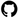
\includegraphics{screenshots/github5.png} \url{https://cmparlettpelleriti.github.io/}

Guy Prochilo {[}screenshots/github5.png{]} \url{http://www.guyprochilo.com/}

\hypertarget{funding}{%
\subsection*{Funding}\label{funding}}
\addcontentsline{toc}{subsection}{Funding}

This work was funded by VIDI Grant 452-17-013 from the Netherlands Organisation for Scientific Research.

\hypertarget{introduction-to-power-analysis}{%
\chapter{Introduction to Power Analysis}\label{introduction-to-power-analysis}}

In this first chapter we will introduce some basic concepts of power analysis. If you are already familiar with these concepts please feel free to move onto the next chapter where we discuss the specifics of how \texttt{Superpower} can used.

\hypertarget{overview-of-power-analysis}{%
\section{Overview of Power Analysis}\label{overview-of-power-analysis}}

The goal of Neyman-Pearson hypothesis testing, often divisively labeled null hypothesis significance testing (NHST), is to determine whether the null hypothesis (\(H_0\)) can be rejected. \emph{Statistical power} is the probability of rejecting the null hypothesis when it is false. And a \emph{power analysis} is a sample size planning procedure performed for a future \emph{yet-to-be-conducted} study that will tell us how many observations are required to reject the null hypothesis with sufficiently high probability.

For example, if you want to plan a study with 80\% power, a power analysis will answer the question:

\begin{quote}
``\emph{If I were to repeat my experiment many thousands of times, what sample size will allow me to reject the null hypothesis on 80\% of these occasions?}''
\end{quote}

Let's illustrate this with an example. Imagine we have conducted a literature review and have estimated that the true standardized mean difference betwen two groups is \(\delta\) = 0.50. That is, the mean of each group differs by 0.50 standard deviations. Assuming that our estimate of this population effect size is accurate, how many observations per group should we collect to reject a null hypothesis of no difference with 80\% probability?

\emph{Probability} is the long-run frequency at which an event occurs (i.e., after many repeated samples). Therefore, we if we want to determine the sample size that allows us to reject the null hypothesis with 80\% probability, we can run a simulation of our study at different sample sizes where each study is repeated many thousands of times. Power will be the proportion of these studies, at each sample size, that reject the null hypothesis.

\begin{Shaded}
\begin{Highlighting}[]
\CommentTok{\# Define our power analysis simulation function}
\NormalTok{power\_sim }\OtherTok{\textless{}{-}} \ControlFlowTok{function}\NormalTok{(n, d, nsims, }\AttributeTok{seed =} \ConstantTok{TRUE}\NormalTok{, }\AttributeTok{print\_plot =} \ConstantTok{TRUE}\NormalTok{)\{}
  
\ControlFlowTok{if}\NormalTok{(seed }\SpecialCharTok{==} \ConstantTok{TRUE}\NormalTok{)\{}\FunctionTok{set.seed}\NormalTok{(}\DecValTok{2}\NormalTok{)\}}
  
\CommentTok{\# For sample size \textasciigrave{}n\textasciigrave{}, we want to perform \textasciigrave{}nsims\textasciigrave{}}
\DocumentationTok{\#\# number of simulations of our experiment using effect size \textasciigrave{}d\textasciigrave{}}
  \FunctionTok{replicate}\NormalTok{(}\AttributeTok{n =}\NormalTok{ nsims, }\AttributeTok{exp =}\NormalTok{ \{}
\NormalTok{    x1 }\OtherTok{=} \FunctionTok{rnorm}\NormalTok{(n, d, }\DecValTok{1}\NormalTok{)}
\NormalTok{    x2 }\OtherTok{=} \FunctionTok{rnorm}\NormalTok{(n, }\DecValTok{0}\NormalTok{, }\DecValTok{1}\NormalTok{)}
    \FunctionTok{t.test}\NormalTok{(}\AttributeTok{x =}\NormalTok{ x1, }\AttributeTok{y =}\NormalTok{ x2, }\AttributeTok{var.equal =} \ConstantTok{TRUE}\NormalTok{)}\SpecialCharTok{$}\NormalTok{p.value\}) }\OtherTok{{-}\textgreater{}}\NormalTok{ ps}

\CommentTok{\# Power for a given \textasciigrave{}n\textasciigrave{} is the long{-}run probability}
\DocumentationTok{\#\# of rejecting the null hypothesis when it is true. }
\CommentTok{\# In our simulation, it is the sum of all  \textasciigrave{}nsims\textasciigrave{} simulations }
\DocumentationTok{\#\# of our study that yield p \textless{} .05 divided by the number of \textasciigrave{}nsims\textasciigrave{} performed. }
\NormalTok{  power }\OtherTok{=} \FunctionTok{sum}\NormalTok{(ps }\SpecialCharTok{\textless{}}\NormalTok{ .}\DecValTok{05}\NormalTok{) }\SpecialCharTok{/}\NormalTok{ nsims}
\NormalTok{  result }\OtherTok{=} \FunctionTok{cbind}\NormalTok{(n, power)}
  
\CommentTok{\# Visualize the results as a plot}
\NormalTok{  ps }\SpecialCharTok{\%\textgreater{}\%} 
    \FunctionTok{as.data.frame}\NormalTok{() }\SpecialCharTok{\%\textgreater{}\%}
    \FunctionTok{ggplot}\NormalTok{(}\FunctionTok{aes}\NormalTok{(}\AttributeTok{x =}\NormalTok{ .)) }\SpecialCharTok{+}
    \FunctionTok{geom\_histogram}\NormalTok{(}\AttributeTok{binwidth =} \FloatTok{0.01}\NormalTok{) }\SpecialCharTok{+}
    \FunctionTok{scale\_x\_continuous}\NormalTok{(}\AttributeTok{breaks =}\NormalTok{ scales}\SpecialCharTok{::}\FunctionTok{pretty\_breaks}\NormalTok{(}\AttributeTok{n =} \DecValTok{15}\NormalTok{)) }\SpecialCharTok{+}
    \FunctionTok{geom\_vline}\NormalTok{(}\AttributeTok{xintercept =} \FloatTok{0.05}\NormalTok{,}
               \AttributeTok{linetype =} \StringTok{"dashed"}\NormalTok{,}
               \AttributeTok{color =} \StringTok{"red"}\NormalTok{) }\SpecialCharTok{+}
    \FunctionTok{xlab}\NormalTok{(}\AttributeTok{label =} \FunctionTok{expression}\NormalTok{(}\FunctionTok{italic}\NormalTok{(p) }\SpecialCharTok{\textasciitilde{}} \StringTok{"value"}\NormalTok{)) }\SpecialCharTok{+}
    \FunctionTok{ylab}\NormalTok{(}\AttributeTok{label =} \StringTok{"Frequency"}\NormalTok{) }\SpecialCharTok{+}
    \FunctionTok{labs}\NormalTok{(}\AttributeTok{caption =} \FunctionTok{paste}\NormalTok{(}
      \StringTok{"Power ="}\NormalTok{,}
\NormalTok{      power }\SpecialCharTok{*} \DecValTok{100}\NormalTok{,}
      \StringTok{"\% }\SpecialCharTok{\textbackslash{}n}\StringTok{"}\NormalTok{,}
      \FunctionTok{sum}\NormalTok{(ps }\SpecialCharTok{\textless{}}\NormalTok{ .}\DecValTok{05}\NormalTok{),}
      \StringTok{"of"}\NormalTok{,}
\NormalTok{      nsims,}
      \StringTok{"simulations yield p \textless{} .05"}
\NormalTok{    )) }\SpecialCharTok{+}
    \FunctionTok{ggtitle}\NormalTok{(}\AttributeTok{label =} \FunctionTok{expr}\NormalTok{(}\FunctionTok{paste}\NormalTok{(}
      \StringTok{"N = "}\NormalTok{,}\SpecialCharTok{!!}\NormalTok{(n }\SpecialCharTok{*} \DecValTok{2}\NormalTok{),}
      \StringTok{" ("}\NormalTok{, n[}\DecValTok{1}\NormalTok{], }\StringTok{" = "}\NormalTok{,}\SpecialCharTok{!!}\NormalTok{n, }\StringTok{"; "}\NormalTok{, n[}\DecValTok{2}\NormalTok{], }\StringTok{" = "}\NormalTok{,}\SpecialCharTok{!!}\NormalTok{n, }\StringTok{")"}
\NormalTok{    ))) }\OtherTok{{-}\textgreater{}}\NormalTok{ pl}
  
  \CommentTok{\# Print our plot}
  \ControlFlowTok{if}\NormalTok{(print\_plot }\SpecialCharTok{==} \ConstantTok{TRUE}\NormalTok{)\{}\FunctionTok{print}\NormalTok{(pl)\}}

  \CommentTok{\# Return the result variable}
  \FunctionTok{return}\NormalTok{(result)}
  
\NormalTok{\}}
\end{Highlighting}
\end{Shaded}

We can use this function to compute power for any given sample size we like. For example, let's determine the power of detecting \(\delta\) = 0.50 if we were to collect \emph{n} = 20 observations per group with 5000 simulations.

\begin{Shaded}
\begin{Highlighting}[]
\FunctionTok{power\_sim}\NormalTok{(}\AttributeTok{n =} \DecValTok{20}\NormalTok{, }\AttributeTok{d =} \FloatTok{0.50}\NormalTok{, }\AttributeTok{nsims =} \DecValTok{5000}\NormalTok{, }\AttributeTok{seed =} \ConstantTok{TRUE}\NormalTok{)}
\end{Highlighting}
\end{Shaded}

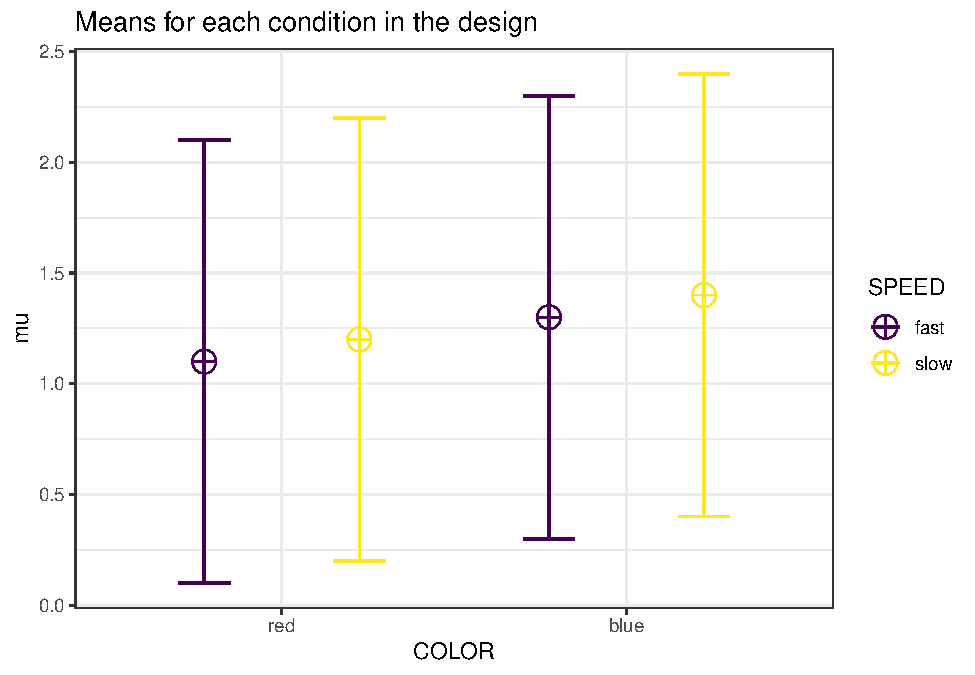
\includegraphics{SuperpowerValidation_files/figure-latex/unnamed-chunk-4-1.pdf}

\begin{verbatim}
##       n  power
## [1,] 20 0.3456
\end{verbatim}

In the above plot, the red dashed line marks \emph{p} = .05. As we can see, the majority of our simulated studies report \emph{p} values greater than .05. In fact, only 1728 of our 5000 simulated studies rejected the null hypothesis with this sample size. Recall that probability is the long-run frequency at which an event occurs (i.e., after many repeated samples), and power is the probability of rejecting the null hypothesis when it is false. If we divide the 1728 correct rejections by the 5000 total simulations we get a final power estimate for this sample size: 34.56\%. That is, after many, many repetitions of our study with a sample size of \emph{n} = 20 per group, we only reject the null hypothesis 34.56\% of the time. If we were planning a study to detect \(\delta\) = 0.50, there is not a high probability that we will reject the null hypothesis with only \emph{n} = 20 per group. We probably wouldn't want to use this sample size.

Let's try \emph{n} = 50 per group.

\begin{Shaded}
\begin{Highlighting}[]
\FunctionTok{power\_sim}\NormalTok{(}\AttributeTok{n =} \DecValTok{50}\NormalTok{, }\AttributeTok{d =} \FloatTok{0.50}\NormalTok{, }\AttributeTok{nsims =} \DecValTok{5000}\NormalTok{, }\AttributeTok{seed =} \ConstantTok{TRUE}\NormalTok{)}
\end{Highlighting}
\end{Shaded}

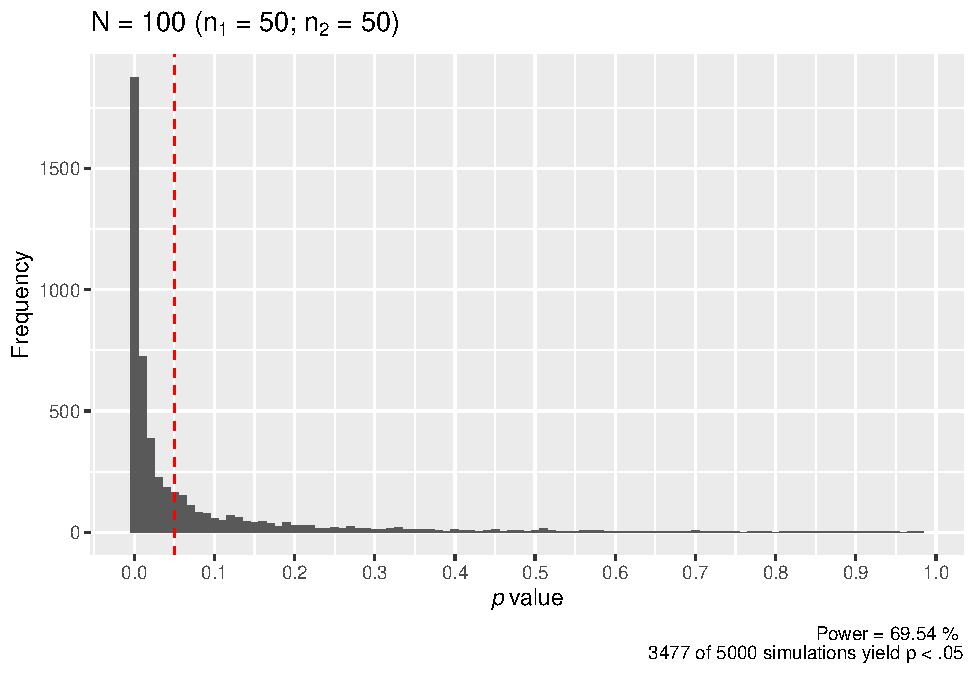
\includegraphics{SuperpowerValidation_files/figure-latex/unnamed-chunk-5-1.pdf}

\begin{verbatim}
##       n  power
## [1,] 50 0.6954
\end{verbatim}

As we can see in the plot of our results, 3477 studies of our 5000 simulated studies rejected the null hypothesis. This corresponds to a power of 69.54\%. Is rejecting the null hypothesis around 70\% of the time satisfactory for you? It isn't for most scientists.

Let's try again with \emph{n} = 80 per group.

\begin{Shaded}
\begin{Highlighting}[]
\FunctionTok{power\_sim}\NormalTok{(}\AttributeTok{n =} \DecValTok{80}\NormalTok{, }\AttributeTok{d =} \FloatTok{0.50}\NormalTok{, }\AttributeTok{nsims =} \DecValTok{5000}\NormalTok{, }\AttributeTok{seed =} \ConstantTok{TRUE}\NormalTok{)}
\end{Highlighting}
\end{Shaded}

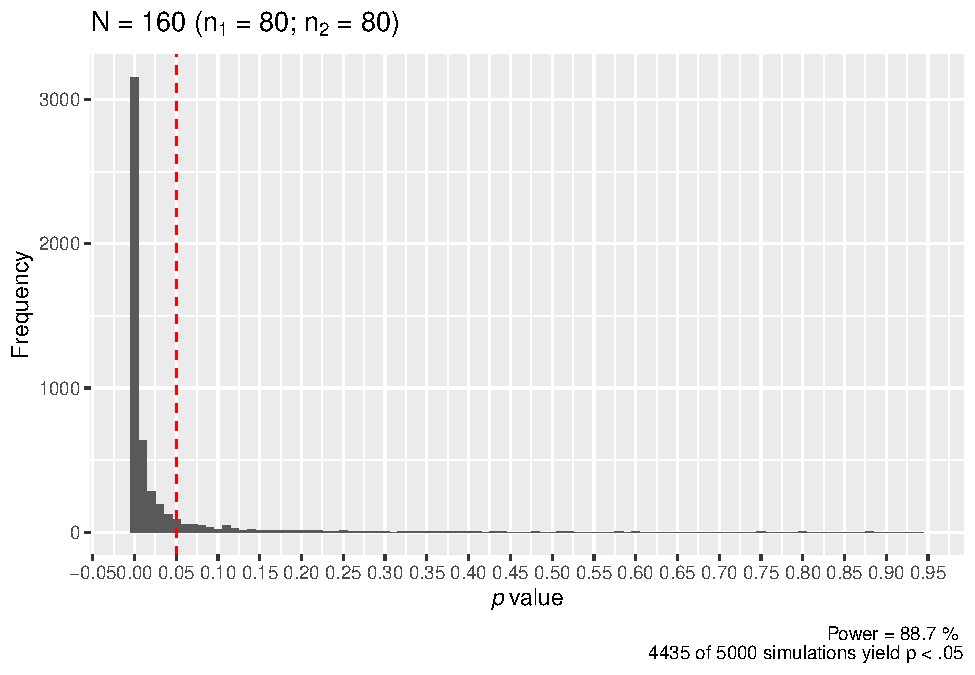
\includegraphics{SuperpowerValidation_files/figure-latex/unnamed-chunk-6-1.pdf}

\begin{verbatim}
##       n power
## [1,] 80 0.887
\end{verbatim}

This time 4435 of our simulated 5000 studies rejected the null hypothesis, corresponding to a power of 88.7\%. This is usually more than enough power for most scientists to consider satisfactory. We might even consider examining power for lower sample sizes.

And that's it. That's all there is to power analysis. Power is simply the probability of rejecting the null hypothesis when it is false. And a power analysis will tell us how many observations are needed to reject this null hypothesis with a sufficiently high probability. Analytic solutions have been determined for many of the common tests you will encounter in psychological science, so simulations like those above are not always necessary. The analytic solution for the \emph{t} test is implemented by the \texttt{pwr::pwr.t.test()} function as part of the \texttt{pwr} package. In fact, if we input the parameters for our last power analysis into \texttt{pwr::pwr.t.test()}, we will obtain almost identical power estimates for \emph{n} = 80 per group:

\begin{Shaded}
\begin{Highlighting}[]
\NormalTok{pwr}\SpecialCharTok{::}\FunctionTok{pwr.t.test}\NormalTok{(}\AttributeTok{n =} \DecValTok{80}\NormalTok{, }\AttributeTok{d =} \FloatTok{0.50}\NormalTok{, }\AttributeTok{sig.level =} \FloatTok{0.05}\NormalTok{)}
\end{Highlighting}
\end{Shaded}

\begin{verbatim}
## 
##      Two-sample t test power calculation 
## 
##               n = 80
##               d = 0.5
##       sig.level = 0.05
##           power = 0.8816025
##     alternative = two.sided
## 
## NOTE: n is number in *each* group
\end{verbatim}

For \emph{n} = 80 per group our simulation reported power = 88.7\%, and the analytic solution reported power = 88.2\%. If we were to increase the number of simulations we performed (perhaps to many hundreds of thousands), these two results would converge even closer.

Power analysis is essential before embarking on any research study. As we will discuss in subsequent section, with high power you are more likely to obtain findings that are trustworthy and you are more likely to draw correct inferences from your results. This is important, not only for getting your findings published, but also for building a reliable literature that is built on cumulative knowledge.

\hypertarget{error-and-power}{%
\section{Error and Power}\label{error-and-power}}

In this Neyman-Pearson framework there are two kinds of errors that we must account for when desiging an experimental study. These are:

\begin{enumerate}
\def\labelenumi{\arabic{enumi}.}
\item
  Type I Error: rejecting the null hypothesis when it is true (also known as false positives or \(\alpha\)).
\item
  Type II Error: failing to reject the null hypothesis when it is true (also known as false negatives or \(\beta\)).
\end{enumerate}

Recall that power is the probability of rejecting the null hypothesis when it is false. This corresponds to \(1-\beta\). Power will depend crucially on sample size, effect size, and the Type I error rates that you are willing to accept.

The typical power analysis parameters in psychology are as follows:

\begin{itemize}
\item
  \(\beta = .20\)

  \begin{itemize}
  \tightlist
  \item
    This means we are willing to make a Type II error 20\% of the time (i.e., 80\% power).
  \end{itemize}
\item
  \(\alpha = .05\)

  \begin{itemize}
  \tightlist
  \item
    This means we are willing to make a Type I error only 5\% of the time (i.e., significance \textless{} .05.
  \end{itemize}
\item
  \(1-\beta = .80\):

  \begin{itemize}
  \tightlist
  \item
    This means we want to be able to correctly reject the null hypothesis, with a effect size \emph{at least as large} as hypothesized, when it is false at least 80\% of the time.
  \end{itemize}
\end{itemize}

The values of each of these parameters reflect our relative concerns regarding the cost of Type I and Type II errors. That is, we regard Type I errors as \emph{four times} more serious than making a Type II error:

\[\frac{\beta}{\alpha} = \frac{.20}{.05} = 4\]
This may not always be the case and we may want to design a study where the errors are balanced:

\[\frac{\beta}{\alpha} = \frac{.05}{.05} = 1\]

And other times we may be willing to increase our Type I error rate slightly in order to reduce the Type II error rate. For example, we may raise our Type I error rate slightly in order to reduce the ratio of errors.

\[\frac{\beta}{\alpha} = \frac{.15}{.075} = 2\]

\hypertarget{effect-size}{%
\section{Effect size}\label{effect-size}}

For any given \(\alpha\) level, the power of a test will increase as the effect size increases. An effect size is a measure of the magnitude of some phenomenon. This might include a measure of the difference between two groups (e.g., the mean), the strength of association between variables (e.g., \emph{r}: the Pearson's correlation coefficient), or the linear relationship between a dependent variable and one or more predictors (e.g., \emph{b}: the unstandardized regression coefficient).

A very common way to quantify effect size in psychological science is Cohen's \emph{d}. This quantity represents the standardized difference between two means. It is computed as:

\[d = \frac{M_1-M_2}{SD_{pool}}\]

Where \(M_1\) is the mean of group one, \(M_2\) is the mean of group two, and \(SD_{pool}\) is the pooled standard deviation of group one and two. Cohen's \emph{d} is sometimes given descriptive labels of small, moderate, and large that correspond to 0.2, 0.5, and 0.8, respectively. However, these descriptives can differ across different measurements. We would strongly advocate against using these ``default'' interpretation scales and instead understand your phenomena/measurements well enough to understand when an effect is meaningful \citep{Caldwell2020}. Some additional common effect sizes alongside their descriptive magnitudes are given in the following table:

\begin{tabu} to \linewidth {>{\raggedright}X>{\raggedleft}X>{\raggedleft}X>{\raggedleft}X}
\hline
Effect & Small & Moderate & Large\\
\hline
*d* & 0.20 & 0.50 & 0.80\\
\hline
*r* & 0.10 & 0.24 & 0.37\\
\hline
*f* & 0.10 & 0.25 & 0.40\\
\hline
$\eta^2$ & 0.01 & 0.06 & 0.14\\
\hline
\end{tabu}

\hypertarget{samp_vs_pop}{%
\section{Sample effect size vs.~population effect size}\label{samp_vs_pop}}

When we run a study what we are doing is collecting a sample of the total population. It follows that any effect sizes computed on the sample data are an \textbf{\emph{estimate of the true population effect size}}. This is an important consideration to keep in mind when performing power analyses. As \citet{albers2018power} demonstrate, researchers are very likely to miss out on interesting effects when studies are powered to detect previously observed effect sizes.

To make this clear, imagine two groups with a known population standardized mean difference of \(Cohen's \ \delta = 0.5\). (We use the Greek symbol \(\delta\) to refer to the population effect size, and the lower case \(d\) to refer to the sample effect size). Now imagine that we have take a random sample of 20 measurements from each of these groups. We can simulate this in R using \texttt{rnorm()}:

\begin{Shaded}
\begin{Highlighting}[]
\CommentTok{\# Set random seed for reproducibility}
\FunctionTok{set.seed}\NormalTok{(}\DecValTok{2}\NormalTok{)}

\CommentTok{\# Simulate datasets with mean difference of 0.5}
\NormalTok{group\_1 }\OtherTok{=} \FunctionTok{rnorm}\NormalTok{(}\AttributeTok{n =} \DecValTok{20}\NormalTok{, }\AttributeTok{mean =} \FloatTok{0.5}\NormalTok{, }\AttributeTok{sd =} \DecValTok{1}\NormalTok{)}
\NormalTok{group\_2 }\OtherTok{=} \FunctionTok{rnorm}\NormalTok{(}\AttributeTok{n =} \DecValTok{20}\NormalTok{, }\AttributeTok{mean =} \DecValTok{0}\NormalTok{, }\AttributeTok{sd =} \DecValTok{1}\NormalTok{)}

\CommentTok{\# Visualize the data}
\FunctionTok{data.frame}\NormalTok{(group\_1, group\_2) }\SpecialCharTok{\%\textgreater{}\%} 
\NormalTok{  tidyr}\SpecialCharTok{::}\FunctionTok{pivot\_longer}\NormalTok{(}
    \AttributeTok{names\_to =} \StringTok{"group"}\NormalTok{, }
    \AttributeTok{values\_to =} \StringTok{"dv"}\NormalTok{, }
    \AttributeTok{cols =} \FunctionTok{everything}\NormalTok{()) }\SpecialCharTok{\%\textgreater{}\%} 
\NormalTok{  GGally}\SpecialCharTok{::}\FunctionTok{ggpairs}\NormalTok{(ggplot2}\SpecialCharTok{::}\FunctionTok{aes}\NormalTok{(}\AttributeTok{colour =}\NormalTok{ group), }
                  \AttributeTok{lower =} \FunctionTok{list}\NormalTok{(}\AttributeTok{combo =} \FunctionTok{wrap}\NormalTok{(ggally\_facethist, }
                                            \AttributeTok{binwidth =} \FloatTok{0.5}\NormalTok{)))}
\end{Highlighting}
\end{Shaded}

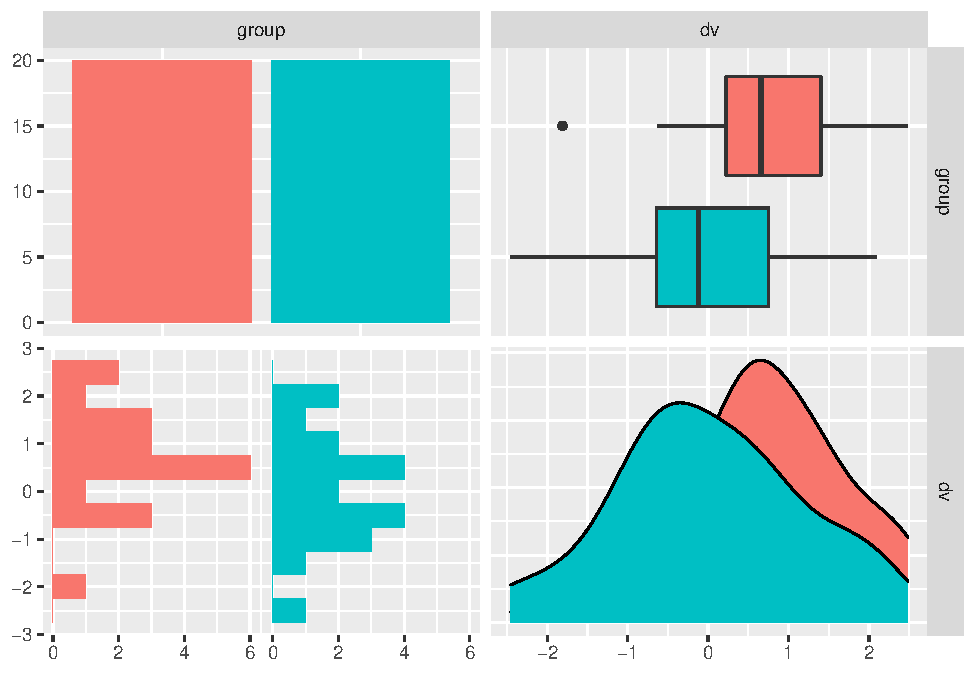
\includegraphics[width=1\linewidth]{SuperpowerValidation_files/figure-latex/unnamed-chunk-9-1}

The above plot visualizes Group 1 (red) and Group 2 (teal) from left to right as: (1) counts, (2) box plots, (3) rotated histograms, and (4) density distributions. We can see clearly that the mean of Group 1 is greater than Group 2.

Now let's compute the sample Cohen's \emph{d} using the formula we described earlier. We will also compute a 95\% CI on Cohen's \emph{d} using the exact method implemented by \texttt{MBESS::ci.smd()}. The 95\% CI will give us all plausible values of Cohen's \(\delta\):

\begin{Shaded}
\begin{Highlighting}[]
\CommentTok{\# Determine N for each group}
\NormalTok{n1 }\OtherTok{=} \FunctionTok{length}\NormalTok{(group\_1)}
\NormalTok{n2 }\OtherTok{=} \FunctionTok{length}\NormalTok{(group\_2)}

\CommentTok{\# Determine standard deviation for each group}
\NormalTok{sd1 }\OtherTok{=} \FunctionTok{sd}\NormalTok{(group\_1)}
\NormalTok{sd2 }\OtherTok{=} \FunctionTok{sd}\NormalTok{(group\_2)}

\CommentTok{\# Compute pooled standard deviation}
\NormalTok{sd\_pool }\OtherTok{=} \FunctionTok{sqrt}\NormalTok{((sd1 }\SpecialCharTok{*}\NormalTok{ sd1 }\SpecialCharTok{*}\NormalTok{ (n1 }\SpecialCharTok{{-}} \DecValTok{1}\NormalTok{) }\SpecialCharTok{+}\NormalTok{ sd2 }\SpecialCharTok{*}\NormalTok{ sd2 }\SpecialCharTok{*}\NormalTok{ (n2 }\SpecialCharTok{{-}} \DecValTok{1}\NormalTok{)) }\SpecialCharTok{/}\NormalTok{ (n1 }\SpecialCharTok{+}\NormalTok{ n2 }\SpecialCharTok{{-}} \DecValTok{2}\NormalTok{))}

\CommentTok{\# Determine the difference between the means}
\NormalTok{m\_diff }\OtherTok{=} \FunctionTok{mean}\NormalTok{(group\_1) }\SpecialCharTok{{-}} \FunctionTok{mean}\NormalTok{(group\_2)}

\CommentTok{\# Compute Cohen\textquotesingle{}s d}
\NormalTok{d }\OtherTok{=}\NormalTok{ m\_diff }\SpecialCharTok{/}\NormalTok{ sd\_pool}

\CommentTok{\# Compute 95\% CI on Cohen\textquotesingle{}s d}
\NormalTok{(}\AttributeTok{d\_ci =}\NormalTok{ MBESS}\SpecialCharTok{::}\FunctionTok{ci.smd}\NormalTok{(}\AttributeTok{smd =}\NormalTok{ d, }\AttributeTok{n.1 =}\NormalTok{ n1, }\AttributeTok{n.2 =}\NormalTok{ n2, }\AttributeTok{conf.level =} \FloatTok{0.95}\NormalTok{))}
\end{Highlighting}
\end{Shaded}

\begin{verbatim}
## $Lower.Conf.Limit.smd
## [1] -0.01853137
## 
## $smd
## [1] 0.6205506
## 
## $Upper.Conf.Limit.smd
## [1] 1.251871
\end{verbatim}

Recall that another name for Cohen's \emph{d} is the standardized mean difference (here, \texttt{smd}). Cohen's \emph{d} on our data is 0.62, and the 95\% CI ranges from -0.02 to 1.25. Let's visualize this as a plot (because we love plots):

\begin{Shaded}
\begin{Highlighting}[]
\CommentTok{\# Plot the result}
\NormalTok{d\_ci }\SpecialCharTok{\%\textgreater{}\%} 
  \FunctionTok{as.data.frame}\NormalTok{() }\SpecialCharTok{\%\textgreater{}\%} 
  \FunctionTok{ggplot}\NormalTok{(}\FunctionTok{aes}\NormalTok{(}\AttributeTok{x =} \StringTok{"Cohen\textquotesingle{}s d"}\NormalTok{)) }\SpecialCharTok{+}
  \FunctionTok{geom\_point}\NormalTok{(}\FunctionTok{aes}\NormalTok{(}\AttributeTok{y =}\NormalTok{ smd)) }\SpecialCharTok{+}
  \FunctionTok{geom\_errorbar}\NormalTok{(}\FunctionTok{aes}\NormalTok{(}\AttributeTok{ymin =}\NormalTok{ Lower.Conf.Limit.smd,}
                    \AttributeTok{ymax =}\NormalTok{ Upper.Conf.Limit.smd), }\AttributeTok{width =} \FloatTok{0.1}\NormalTok{) }\SpecialCharTok{+}
  \FunctionTok{geom\_hline}\NormalTok{(}\AttributeTok{yintercept =} \DecValTok{0}\NormalTok{, }\AttributeTok{linetype =} \StringTok{"dashed"}\NormalTok{) }\SpecialCharTok{+}
  \FunctionTok{theme}\NormalTok{(}\AttributeTok{axis.title.x =} \FunctionTok{element\_blank}\NormalTok{(),}
        \AttributeTok{axis.text.x =} \FunctionTok{element\_blank}\NormalTok{(),}
        \AttributeTok{axis.ticks.x =} \FunctionTok{element\_blank}\NormalTok{()) }\SpecialCharTok{+}
  \FunctionTok{ylab}\NormalTok{(}\AttributeTok{label =} \StringTok{"Cohen\textquotesingle{}s d"}\NormalTok{) }\SpecialCharTok{+}
  \FunctionTok{labs}\NormalTok{(}\AttributeTok{caption =} \StringTok{"Note: Error bar = 95\% CI"}\NormalTok{)}
\end{Highlighting}
\end{Shaded}

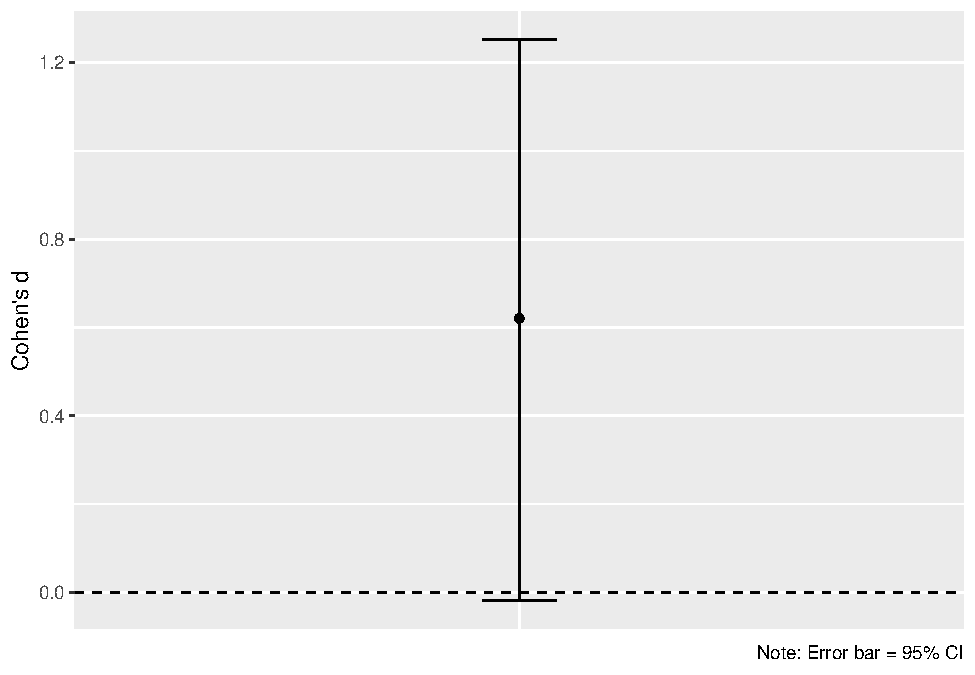
\includegraphics{SuperpowerValidation_files/figure-latex/unnamed-chunk-11-1.pdf}

So what do these results tell us? Although we know with certainty that the population effect size is a Cohen's \(\delta\) of 0.5, our sample effect size is \emph{d} = 0.62. Furthermore, the wide confidence interval on \emph{d} means that our sample effect size has considerable uncertainty. All values in the confidence interval can be considered plausible values for the true population effect size. Indeed, in this unusual situation where we know the population effect size with certainty, we can see that the confidence interval on the sample effect size actually captures the true value (this will not always be the case).

The important take-home message for power analysis is that we want to use \textbf{\emph{population effect size}} and \textbf{\emph{not the sample effect size}} as our effect size input. When we identify sample effect sizes in the literature (which may be through individual studies, meta-analysis, or when appropriate, through internal pilot studies) we must be mindful that the sample effect size may not be equal to the true population effect size. If we were to use the sample effect size in the above example (\emph{d} = 0.62) as our estimate of the population effect size in a power analysis, this would have resulted in much less power than we desired. The sample effect size has \textbf{\emph{overestimated}} the true population effect size. Uncertainty in the population effect size is captured by the 95\% CI on the sample effect size. It is wise to take this into consideration when using previously reported effect sizes for a power analysis.

\hypertarget{safeguard-effect-size}{%
\section{Safeguard Effect Size}\label{safeguard-effect-size}}

Our estimate of the population effect size is an educated guess based on the best information available to us (much like the written hypotheses we have for a study). It's accuracy can have critical implications for the sample size required to attain a certain level of power. For this reason, researchers should routinely consider varying their effect size estimate and assessing the impact this has on their power analysis. If we are using sample effect sizes reported in the literature to estimate the population effect size, one excellent recommendation is to formally consider the uncertainty of sample effect sizes. That is, take into account the 95\% CI on these reported effects.

Consider once again the data reported in the previous section. If you skipped ahead, we simulated a study where the true population effect size was Cohen's \(\delta\) = 0.5. However, we obtained a sample estimate of this effect size as Cohen's \emph{d} = 0.62 in a sample of \emph{N} = 40 observations. Were we to use \emph{d} = 0.62 as our power analysis input, this would result in much less power than anticipated to detect an effect size of \(\delta\) = 0.5. So what should we do?

\citet{Perugini2014} suggest we take into account the uncertainty of the sample effect size. To do so, they suggest for the researcher to compute the lower absolute limit of a 60\% CI on the sample effect. This value would then be used as a \textbf{\emph{safeguard effect size}} and inputted into a power analysis. Why 60\%? Well, the lower limit of a 60\% CI corresponds to a one-sided 80\% CI. As \citet{Perugini2014} describe, this implies a 20\% risk that that the true population effect size is lower than this limit, and correspondingly, 80\% assurance that the population effect size is equal to or greater than this limit. We focus on the lower boundary because of the asymmetry of overestimating compared to underestimating the population effect size in a power analysis.

Let's do this for our previous sample estimate of Cohen's \emph{d}. We can compute a 60\% CI by changing the \texttt{conf.level} parameter to 0.60 in \texttt{MBESS::ci.smd()}:

\begin{Shaded}
\begin{Highlighting}[]
\NormalTok{(}\AttributeTok{d\_safeguard =}\NormalTok{ MBESS}\SpecialCharTok{::}\FunctionTok{ci.smd}\NormalTok{(}\AttributeTok{smd =}\NormalTok{ d, }\AttributeTok{n.1 =}\NormalTok{ n1, }\AttributeTok{n.2 =}\NormalTok{ n2, }\AttributeTok{conf.level =} \FloatTok{0.60}\NormalTok{))}
\end{Highlighting}
\end{Shaded}

\begin{verbatim}
## $Lower.Conf.Limit.smd
## [1] 0.3437032
## 
## $smd
## [1] 0.6205506
## 
## $Upper.Conf.Limit.smd
## [1] 0.8892221
\end{verbatim}

Using our sample Cohen's \emph{d} = 0.62 in a sample of \emph{N} = 40, the lower absolute limit of a 60\% CI on this effect is 0.34. We would therefore use the safeguard sample effect size as our best estimate of the population effect size in our power analysis. While we have somewhat underestimated the population effect size in this scenario, we have also ensured we have sufficient power to detect the population effect size. Sufficient power means we are more likely to draw correct inferences from our data.

\hypertarget{post-hoc-power-analysis}{%
\section{\texorpdfstring{\emph{Post hoc} power analysis}{Post hoc power analysis}}\label{post-hoc-power-analysis}}

All authors of this book are in agreement: \emph{post hoc} power analysis is useless. Many statisticians have made this abundantly clear \citep{gelman2019don, Althouse2021}.

Sometimes editors or reviewers of manuscripts will insist that an author perform a post-experiment power calculation in order to interpret non-significant findings. These \emph{post hoc} or \emph{observed} power calculations are requested on the basis of explaining the observed data rather than planning some future experiment. These analyses are intended to answer the question: \emph{``On the basis of my observed effect size, did I have enough power to reject my null hypothesis?''}. To avoid needless suspense, the answer is always: no.

We will discuss two reasons why \emph{post hoc} power analyses are a problematic practice.

\hypertarget{the-sample-effect-size-is-not-the-population-effect-size}{%
\subsection{\texorpdfstring{The sample effect size is \emph{not} the population effect size}{The sample effect size is not the population effect size}}\label{the-sample-effect-size-is-not-the-population-effect-size}}

As discussed at length in \protect\hyperlink{samp_vs_pop}{previous sections}, the sample effect size is \textbf{\emph{not}} the population effect size. For this simple reason alone, any \emph{post hoc} power calculation will be an inaccurate estimate of the true power of an experiment. To illustrate, consider once more our simulated data set. If you skipped ahead, we simulated random sample of \emph{N} = 40 from two populations (\(n_1\) = 20, \(n_2\) = 20) where the true population effect size was Cohen's \(\delta\) = 0.5. However, based on random sampling alone, we obtained a sample effect size of Cohen's \emph{d} = 0.62.

If we perform a \emph{t}-test on these data, we will find that the data are compatible with the null hypothesis of no difference. That is, \emph{p} \textgreater{} .05. This is exactly the kind of scenario targeted by proponents of \emph{post hoc} power analysis. Let's perform the test:

\begin{Shaded}
\begin{Highlighting}[]
\FunctionTok{t.test}\NormalTok{(}\AttributeTok{x =}\NormalTok{ group\_1, }\AttributeTok{y =}\NormalTok{ group\_2, }\AttributeTok{var.equal =} \ConstantTok{TRUE}\NormalTok{)}
\end{Highlighting}
\end{Shaded}

\begin{verbatim}
## 
##  Two Sample t-test
## 
## data:  group_1 and group_2
## t = 1.9624, df = 38, p-value = 0.05707
## alternative hypothesis: true difference in means is not equal to 0
## 95 percent confidence interval:
##  -0.02199628  1.41348186
## sample estimates:
##     mean of x     mean of y 
##  0.6954610335 -0.0002817572
\end{verbatim}

We obtain \emph{p} = .057. Now let's compute a \emph{post hoc} power calculation on the sample effect size. As will be explained in later sections, we can compute different kinds of power analyses by omitting a single parameter in a power function. Here, we omit \texttt{power} and ask \texttt{pwr::pwr.t.test()} to estimate \texttt{power} on the basis of \emph{n} = 20 per group (total \emph{N} = 40) using \emph{d} = 0.62 and \(\alpha\) = .05 (two-sided):

\begin{Shaded}
\begin{Highlighting}[]
\CommentTok{\# Remind ourselves of the value of Cohen\textquotesingle{}s d for these data:}
\NormalTok{(d)}
\end{Highlighting}
\end{Shaded}

\begin{verbatim}
## [1] 0.6205506
\end{verbatim}

\begin{Shaded}
\begin{Highlighting}[]
\CommentTok{\# Perform the post hoc power analysis}
\DocumentationTok{\#\# by excluding \textasciigrave{}power\textasciigrave{}. }
\DocumentationTok{\#\# Note: \textasciigrave{}n\textasciigrave{} refers to sample size \textquotesingle{}per group\textquotesingle{}:}
\NormalTok{pwr}\SpecialCharTok{::}\FunctionTok{pwr.t.test}\NormalTok{(}\AttributeTok{n =} \DecValTok{20}\NormalTok{, }\AttributeTok{d =}\NormalTok{ d, }\AttributeTok{sig.level =} \FloatTok{0.05}\NormalTok{)}
\end{Highlighting}
\end{Shaded}

\begin{verbatim}
## 
##      Two-sample t test power calculation 
## 
##               n = 20
##               d = 0.6205506
##       sig.level = 0.05
##           power = 0.4811947
##     alternative = two.sided
## 
## NOTE: n is number in *each* group
\end{verbatim}

Our estimate of \emph{post hoc} power is 48\%. However, we know that the true population effect size is \(\delta\) = 0.5. With this knowledge, we can compute the \emph{true} power of our test as:

\begin{Shaded}
\begin{Highlighting}[]
\CommentTok{\# Define delta}
\NormalTok{delta }\OtherTok{=} \FloatTok{0.5}

\CommentTok{\# Perform the post hoc power analysis by excluding \textasciigrave{}power\textasciigrave{}:}
\NormalTok{pwr}\SpecialCharTok{::}\FunctionTok{pwr.t.test}\NormalTok{(}\AttributeTok{n =} \DecValTok{20}\NormalTok{, }\AttributeTok{d =}\NormalTok{ delta, }\AttributeTok{sig.level =} \FloatTok{0.05}\NormalTok{)}
\end{Highlighting}
\end{Shaded}

\begin{verbatim}
## 
##      Two-sample t test power calculation 
## 
##               n = 20
##               d = 0.5
##       sig.level = 0.05
##           power = 0.337939
##     alternative = two.sided
## 
## NOTE: n is number in *each* group
\end{verbatim}

The true power based on the population effect size is 34\%. This is much lower than our \emph{post hoc} power analysis has lead us to believe. As such, \emph{post hoc} power analysis will not tell you whether you had enough power to reject the null hypothesis. That is, unless you are willing to assume your sample effect size \emph{is} the population effect size. This is something a single study cannot tell you. And this is something that is clearly incorrect in our example.

\hypertarget{post-hoc-power-is-merely-a-transformation-of-your-obtained-p-value}{%
\subsection{\texorpdfstring{\emph{Post hoc} power is merely a transformation of your obtained \emph{p} value}{Post hoc power is merely a transformation of your obtained p value}}\label{post-hoc-power-is-merely-a-transformation-of-your-obtained-p-value}}

\emph{Post hoc} power analyses are simply a re-expression of the obtained \emph{p} value. As \citet{Lenth2007} describes, to compute \emph{post hoc} power all we need (beyond our chosen \(\alpha\)) is the \emph{p} value of the test and associated degrees of freedom. For this reason, \emph{post hoc} power does not provide more information than that which is already provided by our \emph{p} value.

Recall from above that our obtained \emph{p} value in our simulated data is .057. \citet{Lenth2007} provides a simple R function to compute \emph{post hoc} power from the obtained \emph{p} value from an independent groups \emph{t} test as follows:

\begin{Shaded}
\begin{Highlighting}[]
\CommentTok{\# Define power function}
\NormalTok{power }\OtherTok{\textless{}{-}} \ControlFlowTok{function}\NormalTok{(p\_val, deg\_f, alpha)\{}

\NormalTok{  delta }\OtherTok{=} \FunctionTok{qt}\NormalTok{(}\AttributeTok{p =} \DecValTok{1} \SpecialCharTok{{-}}\NormalTok{ p\_val }\SpecialCharTok{/} \DecValTok{2}\NormalTok{, }\AttributeTok{df =}\NormalTok{ deg\_f)}
\NormalTok{  crit\_val }\OtherTok{=} \FunctionTok{qt}\NormalTok{(}\AttributeTok{p =} \DecValTok{1} \SpecialCharTok{{-}}\NormalTok{ alpha }\SpecialCharTok{/} \DecValTok{2}\NormalTok{, }\AttributeTok{df =}\NormalTok{ deg\_f)}
\NormalTok{  power }\OtherTok{=} \DecValTok{1} \SpecialCharTok{{-}} \FunctionTok{pt}\NormalTok{(}\AttributeTok{q =}\NormalTok{ crit\_val, }\AttributeTok{df =}\NormalTok{ deg\_f, }\AttributeTok{ncp =}\NormalTok{ delta) }\SpecialCharTok{+} \FunctionTok{pt}\NormalTok{(}\SpecialCharTok{{-}}\NormalTok{crit\_val, deg\_f, delta)}
  
  \FunctionTok{return}\NormalTok{(power)}

\NormalTok{\}}
\end{Highlighting}
\end{Shaded}

Let's apply this function to our obtained \emph{p} value and associated degrees of freedom:

\begin{Shaded}
\begin{Highlighting}[]
\CommentTok{\# Apply power function to our data}
\FunctionTok{power}\NormalTok{(}\AttributeTok{p\_val =} \FloatTok{0.05707}\NormalTok{, }\AttributeTok{deg\_f =} \DecValTok{38}\NormalTok{, }\AttributeTok{alpha =}\NormalTok{ .}\DecValTok{05}\NormalTok{)}
\end{Highlighting}
\end{Shaded}

\begin{verbatim}
## [1] 0.4812096
\end{verbatim}

Using only the obtained \emph{p} value and test degrees of freedom we obtain a \emph{post hoc} power of 48\%. This is identical to our power analysis based on the observed effect size (with error due to rounding of our \emph{p} value). We could do this with any combination of obtained \emph{p} value and degrees of freedom, and obtain exactly the result of a \emph{post hoc} power analysis.

In general, the power of a test yielding exactly \emph{p} = .05 will be around 50\% (and inches ever closer to exactly 50\% as degrees of freedom approaches infinity). If \emph{p} \textgreater{} .05, power (in general) will be less than 50\%. To demonstrate, let's test this with our function using degrees of freedom from five to infinity against \emph{p} values of .05, .10, and .20:

\begin{Shaded}
\begin{Highlighting}[]
\NormalTok{v }\OtherTok{=} \FunctionTok{list}\NormalTok{(}\FunctionTok{seq}\NormalTok{(}\DecValTok{20}\NormalTok{,}\DecValTok{200}\NormalTok{,}\DecValTok{20}\NormalTok{), }\ConstantTok{Inf}\NormalTok{)}
\FunctionTok{map\_df}\NormalTok{(v, }\SpecialCharTok{\textasciitilde{}} \FunctionTok{data.frame}\NormalTok{(., }
                       \FunctionTok{power}\NormalTok{(}\AttributeTok{p\_val =}\NormalTok{ .}\DecValTok{05}\NormalTok{, }\AttributeTok{deg\_f =}\NormalTok{ ., }\AttributeTok{alpha =}\NormalTok{ .}\DecValTok{05}\NormalTok{), }
                       \FunctionTok{power}\NormalTok{(}\AttributeTok{p\_val =} \FloatTok{0.10}\NormalTok{, }\AttributeTok{deg\_f =}\NormalTok{ ., }\AttributeTok{alpha =}\NormalTok{ .}\DecValTok{05}\NormalTok{),}
                       \FunctionTok{power}\NormalTok{(}\AttributeTok{p\_val =} \FloatTok{0.20}\NormalTok{, }\AttributeTok{deg\_f =}\NormalTok{ ., }\AttributeTok{alpha =}\NormalTok{ .}\DecValTok{05}\NormalTok{))) }\SpecialCharTok{\%\textgreater{}\%} 
  \StringTok{\textasciigrave{}}\AttributeTok{colnames\textless{}{-}}\StringTok{\textasciigrave{}}\NormalTok{(}\FunctionTok{c}\NormalTok{(}\StringTok{"Degrees of Freedom"}\NormalTok{, }
                 \StringTok{"Power ($p$ = .05)"}\NormalTok{,}
                 \StringTok{"Power ($p$ = .10)"}\NormalTok{, }
                 \StringTok{"Power ($p$ = .20)"}\NormalTok{)) }\SpecialCharTok{\%\textgreater{}\%} 
\NormalTok{  knitr}\SpecialCharTok{::}\FunctionTok{kable}\NormalTok{(}\AttributeTok{escape =} \ConstantTok{FALSE}\NormalTok{) }\SpecialCharTok{\%\textgreater{}\%} 
\NormalTok{  kableExtra}\SpecialCharTok{::}\FunctionTok{kable\_styling}\NormalTok{(}\AttributeTok{bootstrap\_options =} \StringTok{"striped"}\NormalTok{, }
                            \AttributeTok{full\_width =}\NormalTok{ T, }
                            \AttributeTok{position =} \StringTok{"left"}\NormalTok{)}
\end{Highlighting}
\end{Shaded}

\begin{tabu} to \linewidth {>{\raggedleft}X>{\raggedleft}X>{\raggedleft}X>{\raggedleft}X}
\hline
Degrees of Freedom & Power ($p$ = .05) & Power ($p$ = .10) & Power ($p$ = .20)\\
\hline
20 & 0.5101846 & 0.3754240 & 0.2432919\\
\hline
40 & 0.5050221 & 0.3759611 & 0.2463210\\
\hline
60 & 0.5033422 & 0.3761399 & 0.2473313\\
\hline
80 & 0.5025099 & 0.3762290 & 0.2478362\\
\hline
100 & 0.5020131 & 0.3762824 & 0.2481391\\
\hline
120 & 0.5016829 & 0.3763180 & 0.2483409\\
\hline
140 & 0.5014475 & 0.3763434 & 0.2484851\\
\hline
160 & 0.5012713 & 0.3763624 & 0.2485932\\
\hline
180 & 0.5011344 & 0.3763772 & 0.2486773\\
\hline
200 & 0.5010250 & 0.3763890 & 0.2487446\\
\hline
Inf & 0.5000443 & 0.3764951 & 0.2493496\\
\hline
\end{tabu}

As we can see, whenever a test is non-significant (as it was in our example) the power will usually be less than 50\%. Therefore, whenever you are motivated to perform a \emph{post hoc} power analysis to explain a non-significant result, it is an empty question of whether \emph{post hoc} power is high. The answer, as we alluded to earlier, is always \emph{no}. In our simulated dataset we already knew that \emph{p} \textgreater{} .05, so of course this must mean we had low power. Otherwise we would not have obtained \emph{p} \textgreater{} .05! \emph{Post hoc} power is a mere transformation of the \emph{p} value and provides us with no new information than that we already knew.

Power calculations are useful for designing experiments and planning studies. They are not useful once the data is collected and the final analyses have been completed. Keep this in mind when performing your own power analyses, or attempting to explain non-significant results.

\hypertarget{the-minimal-detectable-effect-size}{%
\section{The Minimal Detectable Effect Size}\label{the-minimal-detectable-effect-size}}

In an ideal world all studies would proceed with sample sizes that give sufficient power to detect population effects. However, we operate within a world of limited resources, and there are often times where researchers are unable to increase sample sizes to attain a specific power. If an experiment is performed in this context, rather than calculating something like \emph{post hoc} power, it is much more informative to compute the smallest effect size that could be detected in a study of this particular sample size. This requires fixing the \(\alpha\) level and sample size, and computing the critical test statistic for the proposed (or conducted) statistical analysis.

We will once again draw on the simulated dataset we introduced \protect\hyperlink{samp_vs_pop}{above}. This dataset was generated by drawing a random sample of \emph{N} = 40 from two populations (\(n_1\) = 20, \(n_2\) = 20) where the true population effect size was Cohen's \(\delta\) = 0.5. However, the obtained sample effect size was Cohen's \emph{d} = 0.62. Furthermore, using an independent groups \emph{t}-test (\(\alpha\) = .05; two-sided) we found that this effect was non-significant (\emph{p} = .057). Let's compute what minimum \emph{t} value was necessary to attain statistical significance. This is the critical \emph{t} value, which can be computed with the \texttt{qt()} function in R:

\begin{Shaded}
\begin{Highlighting}[]
\NormalTok{n1 }\OtherTok{=} \FunctionTok{length}\NormalTok{(group\_1)}
\NormalTok{n2 }\OtherTok{=} \FunctionTok{length}\NormalTok{(group\_2)}
\NormalTok{alpha }\OtherTok{=}\NormalTok{ .}\DecValTok{05}
\NormalTok{deg\_f }\OtherTok{=}\NormalTok{ n1 }\SpecialCharTok{+}\NormalTok{ n2 }\SpecialCharTok{{-}} \DecValTok{2}
\NormalTok{(}\AttributeTok{t\_crit =} \FunctionTok{qt}\NormalTok{(}\AttributeTok{p =} \DecValTok{1} \SpecialCharTok{{-}}\NormalTok{ (alpha}\SpecialCharTok{/}\DecValTok{2}\NormalTok{), }\AttributeTok{df =}\NormalTok{ deg\_f))}
\end{Highlighting}
\end{Shaded}

\begin{verbatim}
## [1] 2.024394
\end{verbatim}

The critical \emph{t} value for our test is 2.024. This means that any obtained \emph{t} statistic lower than this value will yield a statistically non-significant result (i.e., \emph{p} \textgreater{} .05). Our \emph{t} statistic was 1.96, so it is unsurprising that our result was non-significant.

There is an algebraic solution to converting an obtained independent groups \emph{t} statistic (two sample \emph{t}-test) to a Cohen's \emph{d} value:

\[d = t* \sqrt{\frac{1}{n_1} + \frac{1}{n_2}}\]

Here, \emph{t} is the obtained \emph{t} statistic from an independent groups \emph{t} test, and \(n1\) and \(n2\) are the sample sizes of each group, respectively. We can confirm that \emph{d} = 0.62 in our data on the basis of the \emph{t} statistic and sample sizes alone:

\begin{Shaded}
\begin{Highlighting}[]
\CommentTok{\# Store the t test result}
\NormalTok{result }\OtherTok{=} \FunctionTok{t.test}\NormalTok{(}\AttributeTok{x =}\NormalTok{ group\_1, }\AttributeTok{y =}\NormalTok{ group\_2, }\AttributeTok{var.equal =} \ConstantTok{TRUE}\NormalTok{)}

\CommentTok{\# Extract the t value}
\NormalTok{(}\AttributeTok{t\_val =} \FunctionTok{as.numeric}\NormalTok{(result}\SpecialCharTok{$}\NormalTok{statistic))}
\end{Highlighting}
\end{Shaded}

\begin{verbatim}
## [1] 1.962353
\end{verbatim}

\begin{Shaded}
\begin{Highlighting}[]
\CommentTok{\# Store the sample size of each group}
\NormalTok{n1 }\OtherTok{=} \FunctionTok{length}\NormalTok{(group\_1)}
\NormalTok{n2 }\OtherTok{=} \FunctionTok{length}\NormalTok{(group\_2)}

\CommentTok{\# Compute Cohen\textquotesingle{}s d from the t statistic }
\DocumentationTok{\#\# and sample sizes alone}
\NormalTok{t\_val }\SpecialCharTok{*} \FunctionTok{sqrt}\NormalTok{((}\DecValTok{1}\SpecialCharTok{/}\NormalTok{n1 }\SpecialCharTok{+} \DecValTok{1}\SpecialCharTok{/}\NormalTok{n2))}
\end{Highlighting}
\end{Shaded}

\begin{verbatim}
## [1] 0.6205506
\end{verbatim}

\emph{d} = 0.62. Magic. We can take advantage of this formula and, instead of inputting the obtained \emph{t} statistic, we can input the critical \emph{t} statistic for a study of this size. In doing so, we will obtain a critical \emph{d} value:

\begin{Shaded}
\begin{Highlighting}[]
\CommentTok{\# Remind ourselves of what t\_crit is}
\NormalTok{(t\_crit)}
\end{Highlighting}
\end{Shaded}

\begin{verbatim}
## [1] 2.024394
\end{verbatim}

\begin{Shaded}
\begin{Highlighting}[]
\CommentTok{\# Compute the critical d value}
\NormalTok{t\_crit }\SpecialCharTok{*} \FunctionTok{sqrt}\NormalTok{((}\DecValTok{1}\SpecialCharTok{/}\NormalTok{n1 }\SpecialCharTok{+} \DecValTok{1}\SpecialCharTok{/}\NormalTok{n2))}
\end{Highlighting}
\end{Shaded}

\begin{verbatim}
## [1] 0.6401696
\end{verbatim}

In a study of this size the critical \emph{d} value is 0.64. This means that any obtained \emph{d} statistic lower or equal to this value will yield a non-significant result (i.e., \emph{p} \textgreater{} .05). As we obtained \emph{d} = 0.62 as our sample effect size, it is unsurprising that our result is non-significant. The critical \emph{d} value of 0.64 is the minimal detectable effect size in a study of this size.

What does this all mean? Well, if a researcher believes that the true population effect size is less than 0.62 (perhaps, \(\delta\) = 0.5), they should be un-surprised if they find a non-significant finding in \emph{N} = 40. The minimum effect size they could have hoped to have detected was \emph{d} = 0.66. The non-significant result is explained by the fact that a study of this sample size cannot detect effect sizes below the critical \emph{d} value. In later chapters we will discuss how to use \texttt{Superpower} to address these issues using tools such as the \texttt{plot\_power} function and the \texttt{morey\_plot} functions.

\hypertarget{the-experimental-design}{%
\chapter{The Experimental Design}\label{the-experimental-design}}

Now that we have introduced the basics of what constitutes a power analysis we can move onto how to use \texttt{Superpower} as tool for power analyses. The first step is to define and specify the details of the experimental design. Currently, \texttt{Superpower} only provides power analysis capabilities for ANOVAs (and MANOVA for repeated measures) so all designs are currently defined by the \texttt{ANOVA\_design} function.

\hypertarget{anova_design-function}{%
\section{ANOVA\_design function}\label{anova_design-function}}

Currently the \texttt{ANOVA\_design} function can create designs with up to three factors, for both within, between, and mixed designs. It requires the following input: design, n, mu, sd, r, and optionally allows you to set \texttt{labelnames}.

\begin{enumerate}
\def\labelenumi{\arabic{enumi}.}
\tightlist
\item
  \texttt{design}: string that specifies the design (see below).
\item
  \texttt{n}: the sample size for each between subject condition. Can be specified as a single value (when all conditions have the same sample size), or as a vector of values specifying the sample size for each condition.
\item
  \texttt{mu}: a vector with the means for each condition.
\item
  \texttt{sd}: the population standard deviation. Assumes homogeneity of variances (only one standard deviation can be provided). Can be specified as a single value (when all conditions have the same standard deviation), or as a vector of values specifying the standard deviation for each condition.
\item
  \texttt{r}: the correlation(s) for within designs (or 0 for between designs). Can be specified as a single value (when all pairs of variables have the same correlation), or as a correlation matrix specifying the correlation between each pair.
\item
  \texttt{labelnames}: This is an optional vector of words that indicates factor names and level names (see below).
\item
  A final optional setting is to specify if you want to automatically print a plot or not (\texttt{plot} = TRUE or FALSE)
\end{enumerate}

\hypertarget{specifying-the-design-using-design}{%
\subsection{\texorpdfstring{Specifying the design using \texttt{design}}{Specifying the design using design}}\label{specifying-the-design-using-design}}

The \texttt{design} option is used to specify the design.
Every factor is specified with a number, indicating the number of levels of the factor, and a letter, b or w, to indicate whether the factor is manipulated between or within participants.
For example, a \texttt{2b} design has two between-participant groups.
A \texttt{12w} design has one factor with 12 levels, all manipulated within-participants.
A \texttt{2b*3w} is a design with two factors (a 2b factor and a 3w factor), the first of which has 2 between participant levels (2b), and the second of which has 3 within participants levels (3w).
\textbf{If there are multiple factors (the functions take up to three different factors) separate factors with a * (asterisk)}.
An example of a \texttt{2b*3w} design is a group of people in one condition who get a drug, and a group of people in another condition who get a placebo (hence \texttt{2b}), and we measure their health before they take the pill, one day after they take the pill, and a week after they take the pill (hence the \texttt{3w}).

\hypertarget{specifying-the-means-using-mu}{%
\subsection{\texorpdfstring{Specifying the means using \texttt{mu}}{Specifying the means using mu}}\label{specifying-the-means-using-mu}}

Note that for each cell in the design, a mean must be provided. Thus, for a \texttt{2b*3w} design, \textbf{6} (i.e., 2*3=6) means need to be entered.

Means need to be entered in the correct order. ANOVA\_design outputs a plot so you can check if you entered all means as you intended. Always carefully check if the plot that is generated matches your expectations.

The general principle is that the code generates factors, indicated by the factor names you entered in the labelnames variable, (i.e., \emph{condition} and \emph{time}). Levels are indicated by factor names and levels (e.g., control\_time1, control\_time2, control\_time3, etc).

If your design has just one factor, just enter the means in the same order as the labelnames (see below). For more factors, note the general pattern in the example below. Means are entered in the following order for a 3 factors design (each with 2 levels):

\begin{enumerate}
\def\labelenumi{\arabic{enumi}.}
\tightlist
\item
  a1 b1 c1
\item
  a1 b1 c2
\item
  a1 b2 c1
\item
  a1 b2 c2
\item
  a2 b1 c1
\item
  a2 b1 c2
\item
  a2 b2 c1
\item
  a2 b2 c2
\end{enumerate}

So if you enter the means 1, 2, 3, 4, 5, 6, 7, 8 the first 4 means correspond to level 1 of factor 1, the second 4 means correspond to level 2 of factor 1. Within the first 4 means, the first 2 correspond to level 1 of factor 2, and within those 2 means, the first corresponds to level 1 of factor 3.

The plot below visualizes means from 1 to 8 being entered in a vector: \texttt{mu\ =\ c(1,\ 2,\ 3,\ 4,\ 5,\ 6,\ 7,\ 8)} so you can see how the basic ordering works.

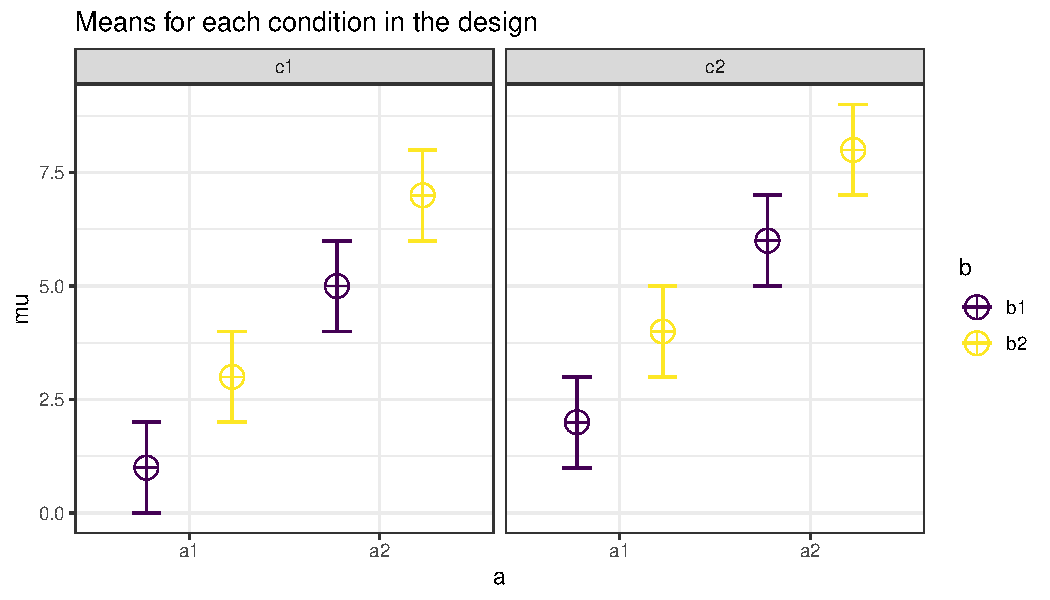
\includegraphics{SuperpowerValidation_files/figure-latex/unnamed-chunk-22-1.pdf}

\hypertarget{specifying-label-names}{%
\subsection{Specifying label names}\label{specifying-label-names}}

To make sure the plots and tables with simulation results are easy to interpret, it really helps to name all factors and levels. You can enter the labels in the `labelnames' variable. You can also choose not to specify names. Then all factors are indicated by letters (a, b, c) and all levels by numbers (a1, a2, a3).

For the 2x3 design we have been using as an example, where there are 2 factors (condition and time of measurement), the first with 2 levels (placebo vs.~medicine) and the second with three levels (time1, time2, and time3) we would enter the labels as follows:

\texttt{c("condition",\ "placebo",\ "medicine",\ "time",\ "time1",\ "time2",\ "time3")}

As you can see, you follow the order of the design (\texttt{2b*3w}), and first write the \textbf{FACTOR} label (condition) followed by the levels of that factor (placebo and medicine). Then you write the second factor name (time) followed by the three labels for each \textbf{LEVEL} (time1, time2, time3). \textbf{Do not use spaces or special characters in the names (so not ``time 1'' or ``time\_1'' but ``time1'').}

Some examples:

\begin{enumerate}
\def\labelenumi{\arabic{enumi}.}
\tightlist
\item
  One within factor (time with 2 levels), 2w: \texttt{c("time",\ "morning",\ "evening")}
\item
  Two between factors (time and group, each with 2 levels), 2b*2b: \texttt{c("time",\ "morning",\ "evening",\ "group",\ "control",\ "experimental")}
\item
  Two between factors (time and group, first with 4 levels, second with 2 levels), 4b*2b: \texttt{c("time",\ "morning",\ "afternoon"\ ,"evening",\ "night",\ "group",\ "control",\ "experimental")}
\end{enumerate}

\hypertarget{specifying-the-correlation}{%
\subsection{Specifying the correlation}\label{specifying-the-correlation}}

Depending on whether factors are manipulated within or between, variables are correlated, or not. You can set the correlation for within-participant factors. You can either assume all factors have the same correlation (e.g., r = 0.7), or enter the correlations for each pair of observations separately by specifying a correlation matrix.

In a 2x2 design, with factors A and B, each with 2 levels, there are 6 possible comparisons that can be made.

\begin{enumerate}
\def\labelenumi{\arabic{enumi}.}
\tightlist
\item
  A1 vs A2
\item
  A1 vs B1
\item
  A1 vs B2
\item
  A2 vs B1
\item
  A2 vs B2
\item
  B1 vs B2
\end{enumerate}

The number of possible comparisons is the product of the levels of all factors squared minus the product of all factors, divided by two. For a 2x2 design where each factor has two levels, this is:

\begin{Shaded}
\begin{Highlighting}[]
\NormalTok{(((}\DecValTok{2} \SpecialCharTok{*} \DecValTok{2}\NormalTok{) }\SpecialCharTok{\^{}} \DecValTok{2}\NormalTok{) }\SpecialCharTok{{-}}\NormalTok{ (}\DecValTok{2} \SpecialCharTok{*} \DecValTok{2}\NormalTok{))}\SpecialCharTok{/}\DecValTok{2}
\end{Highlighting}
\end{Shaded}

\begin{verbatim}
## [1] 6
\end{verbatim}

The number of possible comparisons increases rapidly when adding factors and levels for each factor. For example, for a 2x2x4 design it is:

\begin{Shaded}
\begin{Highlighting}[]
\NormalTok{(((}\DecValTok{2} \SpecialCharTok{*} \DecValTok{2} \SpecialCharTok{*} \DecValTok{4}\NormalTok{) }\SpecialCharTok{\^{}} \DecValTok{2}\NormalTok{) }\SpecialCharTok{{-}}\NormalTok{ (}\DecValTok{2} \SpecialCharTok{*} \DecValTok{2} \SpecialCharTok{*} \DecValTok{4}\NormalTok{))}\SpecialCharTok{/}\DecValTok{2}
\end{Highlighting}
\end{Shaded}

\begin{verbatim}
## [1] 120
\end{verbatim}

Each of these comparisons can have their own correlation if the factor is manipulated within subjects (if the factor is manipulated between subjects the correlation is 0).
These correlations determine the covariance matrix.
Potvin and Schutz (2000) surveyed statistical tools for power analysis and conclude that most software packages are limited to one factor repeated measure designs and do not provide power calculations for within designs with multiple factor (which is still true for software such as G*Power).
Furthermore, software solutions which were available at the time (DATASIM by Bradley, Russel, \& Reeve, 1996) required researchers to assume correlations were of the same magnitude for all within factors, which is not always realistic.
If you do not want to assume equal correlations for all paired comparisons, you can specify the correlation for each possible comparison.

The order in which the correlations are entered in the vector should match the covariance matrix.
The order for a 2x2 design is given in the 6 item list above. The general pattern is that the matrix is filled from top to bottom, and left to right, illustrated by the increasing correlations in the table below.
The diagonal is generated dynamically (based on the standard deviation).

\begin{table}

\caption{\label{tab:unnamed-chunk-25}Correlation Matrix}
\centering
\begin{tabular}[t]{l|r|r|r|r}
\hline
  & a1\_b1 & a1\_b2 & a2\_b1 & a2\_b2\\
\hline
a1\_b1 & 1.00 & 0.91 & 0.92 & 0.93\\
\hline
a1\_b2 & 0.91 & 1.00 & 0.94 & 0.95\\
\hline
a2\_b1 & 0.92 & 0.94 & 1.00 & 0.96\\
\hline
a2\_b2 & 0.93 & 0.95 & 0.96 & 1.00\\
\hline
\end{tabular}
\end{table}

\newpage

We would enter this correlation matrix in the \texttt{ANOVA\_design} function as:

\begin{Shaded}
\begin{Highlighting}[]
\NormalTok{design\_result }\OtherTok{\textless{}{-}} \FunctionTok{ANOVA\_design}\NormalTok{(}\AttributeTok{design =} \StringTok{"2w*2w"}\NormalTok{,}
                              \AttributeTok{n =} \DecValTok{80}\NormalTok{,}
                              \AttributeTok{mu =} \FunctionTok{c}\NormalTok{(}\FloatTok{1.1}\NormalTok{, }\FloatTok{1.2}\NormalTok{,}
                                     \FloatTok{1.3}\NormalTok{, }\FloatTok{1.4}\NormalTok{),}
                              \AttributeTok{sd =} \DecValTok{1}\NormalTok{,}
\NormalTok{                              r }\OtherTok{\textless{}{-}} \FunctionTok{c}\NormalTok{(}\FloatTok{0.91}\NormalTok{, }\FloatTok{0.92}\NormalTok{,}
                                     \FloatTok{0.93}\NormalTok{, }\FloatTok{0.94}\NormalTok{,}
                                     \FloatTok{0.95}\NormalTok{, }\FloatTok{0.96}\NormalTok{),}
                              \AttributeTok{labelnames =} \FunctionTok{c}\NormalTok{(}\StringTok{"COLOR"}\NormalTok{,}
                                             \StringTok{"red"}\NormalTok{, }\StringTok{"blue"}\NormalTok{,}
                                             \StringTok{"SPEED"}\NormalTok{,}
                                             \StringTok{"fast"}\NormalTok{, }\StringTok{"slow"}\NormalTok{),}
                              \AttributeTok{plot =} \ConstantTok{TRUE}\NormalTok{)}
\end{Highlighting}
\end{Shaded}

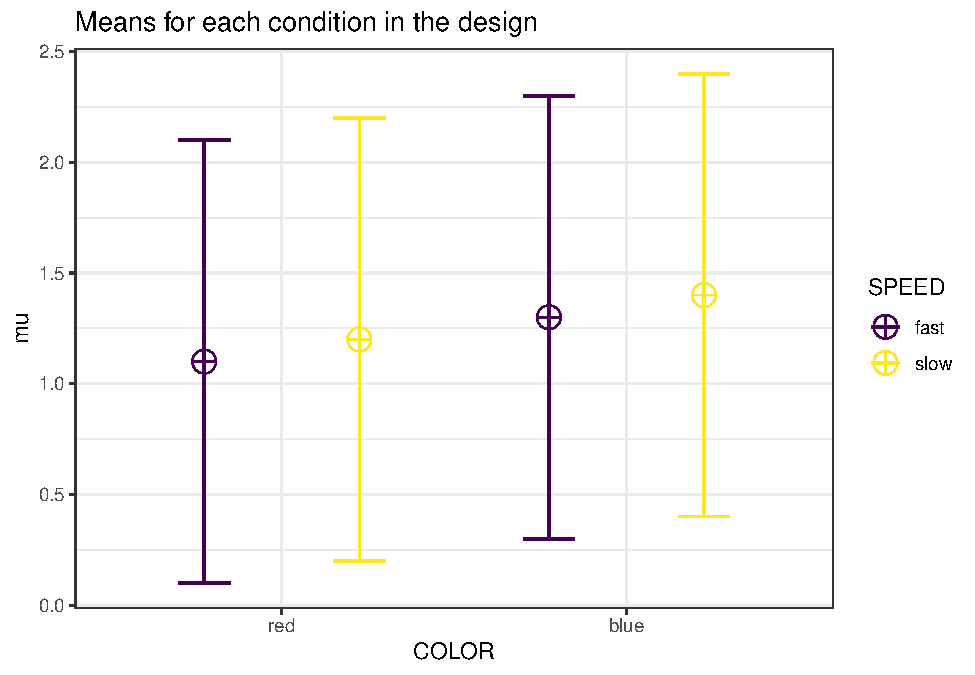
\includegraphics{SuperpowerValidation_files/figure-latex/unnamed-chunk-26-1.pdf}

\newpage

We can check the correlation matrix by printing it from the design\_result object to check if it was entered the way we wanted:

\begin{Shaded}
\begin{Highlighting}[]
\NormalTok{design\_result}\SpecialCharTok{$}\NormalTok{cor\_mat}
\end{Highlighting}
\end{Shaded}

\begin{table}[!h]

\caption{\label{tab:unnamed-chunk-28}Correlation Matrix}
\centering
\begin{tabular}[t]{l|r|r|r|r}
\hline
  & red\_fast & red\_slow & blue\_fast & blue\_slow\\
\hline
red\_fast & 1.00 & 0.91 & 0.92 & 0.93\\
\hline
red\_slow & 0.91 & 1.00 & 0.94 & 0.95\\
\hline
blue\_fast & 0.92 & 0.94 & 1.00 & 0.96\\
\hline
blue\_slow & 0.93 & 0.95 & 0.96 & 1.00\\
\hline
\end{tabular}
\end{table}

We should also check the covariance-variance matrix to ensure the \texttt{ANOVA\_design} function is working properly.
The variance should be the diagonal element while the off-diagonal elements should be equal to \texttt{covariance\ =\ correlation*variance} or \(cov_{x,y}=\frac{\sum_{i=1}^{N}(x_{i}-\bar{x})(y_{i}-\bar{y})}{N-1}\).
In this case, it is identical to the correlation matrix because the variance is equal to 1.

\begin{Shaded}
\begin{Highlighting}[]
\NormalTok{design\_result}\SpecialCharTok{$}\NormalTok{sigmatrix}
\end{Highlighting}
\end{Shaded}

\begin{table}[!h]

\caption{\label{tab:unnamed-chunk-30}Covariance-Variance Matrix}
\centering
\begin{tabular}[t]{l|r|r|r|r}
\hline
  & red\_fast & red\_slow & blue\_fast & blue\_slow\\
\hline
red\_fast & 1.00 & 0.91 & 0.92 & 0.93\\
\hline
red\_slow & 0.91 & 1.00 & 0.94 & 0.95\\
\hline
blue\_fast & 0.92 & 0.94 & 1.00 & 0.96\\
\hline
blue\_slow & 0.93 & 0.95 & 0.96 & 1.00\\
\hline
\end{tabular}
\end{table}

\hypertarget{specifying-the-sample-size}{%
\subsection{Specifying the sample size}\label{specifying-the-sample-size}}

You can set the sample size \textbf{per condition} by setting a value for \texttt{n}.
It is beneficial to have a fully balanced design (the same sample size in each condition) in case of any violations of assumptions (such as homogeneity of variances), but this might not always be possible in real life, and it can be more efficient to collect a larger sample size in some conditions (e.g., if the population from which other participants are drawn is more difficult to collect).
Superpower allows you to enter a single value (the same sample size in each condition) or a vector of values (different sample sizes in each condition).

This means for the \texttt{2w*2w} design above there is a total of 80 participants/subjects with a total of 320 observations.
Instead of 80 participants in each condition, for a \texttt{2b*2b} between subjects design, we could also specify the sample size as \texttt{n\ =\ c(60,\ 80,\ 80,\ 60)} if we plan to collect 60 participants in 2 conditions and 80 participants in 2 other conditions.

\hypertarget{specifying-the-standard-deviation}{%
\subsection{Specifying the standard deviation}\label{specifying-the-standard-deviation}}

You can set the standard deviation(s) by setting a value of \texttt{sd}.
You can enter either a single standard deviation for all conditions, or you can \textbf{violate the assumption of homogeneity of variance} by entering a vector with different standard deviations for each conditions (e.g., \texttt{sd\ =\ c(0.8,\ 1.2,\ 0.92,\ 1.12)} for a \texttt{2b*2b} design.
Violation the homogeneity of variances assumption will affect the type I error rate if the differences in \texttt{sd} between conditions are extreme.
Note that there is always some uncertainty in which values you can expect in the study you are planning.
It is therefore useful to perform sensitivity analyses (e.g., running the simulation with the expected standard deviation, but also with more conservative or even worst-case-scenario values).

\hypertarget{one-way-anova}{%
\chapter{One-Way ANOVA}\label{one-way-anova}}

\hypertarget{introduction}{%
\section{Introduction}\label{introduction}}

Using the formula also used by \citet{albers2018power}, we can determine the means that should yield a specified effect sizes (expressed in Cohen's \emph{f}). Eta-squared (identical to partial eta-squared for one-way ANOVA's) has benchmarks of .0099, .0588, and .1379 for small, medium, and large effect sizes \citep{cohen1988spa}. Although these benchmarks are quite arbitrary, and researchers should only use such benchmarks for power analyses as a last resort, we will demonstrate an a priori power analysis for these values.

\hypertarget{two-conditions}{%
\subsection{Two conditions}\label{two-conditions}}

Imagine we aim to design a study to test the hypothesis that giving people a pet to take care of will increase their life satisfaction. We have a control condition, and a condition where people get a pet, and randomly assign participants to either condition. We can simulate a one-way ANOVA with a specified alpha, sample size, and effect size, on see the statistical power we would have for the ANOVA and the follow-up comparisons. We expect pets to increase life-satisfaction compared to the control condition. Based on work by \citet{pavot1993affective} we believe that we can expect responses on the life-satifaction scale to have a mean of approximately 24 in our population, with a standard deviation of 6.4. We expect having a pet increases life satisfaction with approximately 2.2 scale points for participants who get a pet. There are 200 participants in total, with 100 participants in each condition. But before we proceed with the data collection, we examine the statistical power our design would have to detect the differences we predict.

\begin{Shaded}
\begin{Highlighting}[]
\NormalTok{string }\OtherTok{\textless{}{-}} \StringTok{"2b"}
\NormalTok{n }\OtherTok{\textless{}{-}} \DecValTok{100}
\CommentTok{\# We are thinking of running 100 people in each condition}
\NormalTok{mu }\OtherTok{\textless{}{-}} \FunctionTok{c}\NormalTok{(}\DecValTok{24}\NormalTok{, }\FloatTok{26.2}\NormalTok{)}
\CommentTok{\# Enter means in the order that matches the labels below.}
\CommentTok{\# In this case, control, pet.}
\NormalTok{sd }\OtherTok{\textless{}{-}} \FloatTok{6.4}
\NormalTok{labelnames }\OtherTok{\textless{}{-}} \FunctionTok{c}\NormalTok{(}\StringTok{"condition"}\NormalTok{, }\StringTok{"control"}\NormalTok{, }\StringTok{"pet"}\NormalTok{) }\CommentTok{\#}
\CommentTok{\# the label names should be in the order of the means specified above.}
\NormalTok{design\_result }\OtherTok{\textless{}{-}} \FunctionTok{ANOVA\_design}\NormalTok{(}\AttributeTok{design =}\NormalTok{ string,}
                   \AttributeTok{n =}\NormalTok{ n,}
                   \AttributeTok{mu =}\NormalTok{ mu,}
                   \AttributeTok{sd =}\NormalTok{ sd,}
                   \AttributeTok{labelnames =}\NormalTok{ labelnames)}
\end{Highlighting}
\end{Shaded}

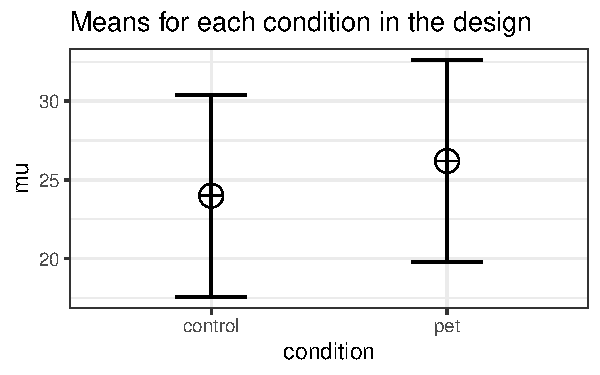
\includegraphics{SuperpowerValidation_files/figure-latex/start_one_way-1.pdf}

\begin{Shaded}
\begin{Highlighting}[]
\NormalTok{alpha\_level }\OtherTok{\textless{}{-}} \FloatTok{0.05}
\CommentTok{\# You should think carefully about how to justify your alpha level.}
\CommentTok{\# We will use 0.05 in most examples, but do not support using a 0.05 alpha level for all analyses.}
\end{Highlighting}
\end{Shaded}

\begin{Shaded}
\begin{Highlighting}[]
\NormalTok{simulation\_result }\OtherTok{\textless{}{-}} \FunctionTok{ANOVA\_power}\NormalTok{(design\_result,}
                                 \AttributeTok{alpha\_level =}\NormalTok{ alpha\_level,}
                                 \AttributeTok{nsims =}\NormalTok{ nsims,}
                                 \AttributeTok{verbose =} \ConstantTok{FALSE}\NormalTok{)}
\end{Highlighting}
\end{Shaded}

\begin{table}[!h]

\caption{\label{tab:unnamed-chunk-33}Simulated ANOVA Result}
\centering
\begin{tabular}[t]{l|r|r}
\hline
  & power & effect\_size\\
\hline
anova\_condition & 67.79 & 0.0335176\\
\hline
\end{tabular}
\end{table}

\begin{Shaded}
\begin{Highlighting}[]
\NormalTok{exact\_result }\OtherTok{\textless{}{-}} \FunctionTok{ANOVA\_exact}\NormalTok{(design\_result,}
                            \AttributeTok{alpha\_level =}\NormalTok{ alpha\_level,}
                            \AttributeTok{verbose =} \ConstantTok{FALSE}\NormalTok{)}
\end{Highlighting}
\end{Shaded}

\begin{table}[!h]

\caption{\label{tab:unnamed-chunk-35}Exact ANOVA Result}
\centering
\begin{tabular}[t]{l|r|r|r|r}
\hline
  & power & partial\_eta\_squared & cohen\_f & non\_centrality\\
\hline
condition & 67.68572 & 0.0289748 & 0.1727409 & 5.908203\\
\hline
\end{tabular}
\end{table}

The result shows that we have exactly the same power for the ANOVA (note: in the simulation, values will differ slightly, but with a large number of simulations, power estimates will be identical), as we have for the \emph{t}-test. When there are only two groups, these tests are mathematically identical. In a study with 100 participants, we would have quite low power (around 67.7\%). An ANOVA with 2 groups is identical to a \emph{t}-test. For our example, Cohen's d (the standardized mean difference) is 2.2/6.4, or d = 0.34375 for the difference between the control condition and pets, which we can use to easily compute the expected power for these simple comparisons using the \texttt{pwr} \citeyearpar{R-pwr} package.

\begin{Shaded}
\begin{Highlighting}[]
\FunctionTok{pwr.t.test}\NormalTok{(}\AttributeTok{d =} \FloatTok{2.2}\SpecialCharTok{/}\FloatTok{6.4}\NormalTok{,}
           \AttributeTok{n =} \DecValTok{100}\NormalTok{,}
           \AttributeTok{sig.level =} \FloatTok{0.05}\NormalTok{,}
           \AttributeTok{type =} \StringTok{"two.sample"}\NormalTok{,}
           \AttributeTok{alternative =} \StringTok{"two.sided"}\NormalTok{)}\SpecialCharTok{$}\NormalTok{power}
\end{Highlighting}
\end{Shaded}

\begin{verbatim}
## [1] 0.6768572
\end{verbatim}

We can also directly compute Cohen's \emph{f} from Cohen's d for two groups, as \citet{cohen1988spa} describes, because \emph{f} = 1/2d. So \emph{f} = 0.5*0.34375 = 0.171875. And indeed, power analysis using the pwr package yields the same result using the \texttt{pwr.anova.test} as the \texttt{power.t.test}.

\begin{Shaded}
\begin{Highlighting}[]
\NormalTok{K }\OtherTok{\textless{}{-}} \DecValTok{2}
\NormalTok{n }\OtherTok{\textless{}{-}} \DecValTok{100}
\NormalTok{f }\OtherTok{\textless{}{-}} \FloatTok{0.171875}
\FunctionTok{pwr.anova.test}\NormalTok{(}\AttributeTok{n =}\NormalTok{ n,}
               \AttributeTok{k =}\NormalTok{ K,}
               \AttributeTok{f =}\NormalTok{ f,}
               \AttributeTok{sig.level =}\NormalTok{ alpha\_level)}\SpecialCharTok{$}\NormalTok{power}
\end{Highlighting}
\end{Shaded}

\begin{verbatim}
## [1] 0.6768572
\end{verbatim}

This analysis tells us that running the study with 100 participants in each condition is very likely to \emph{not} yield a significant test result, even if our expected pattern of differences is true. This is not optimal.

Let's mathematically explore which pattern of means we would need to expect to have 90\% power for the ANOVA with 100 participants in each group. We can use the pwr package in R to compute a sensitivity analysis that tells us the effect size, in Cohen's \emph{f}, that we are able to detect with 2 groups and 100 participants in each group, in order to achieve 90\% power with an alpha level of 5\%.

\begin{Shaded}
\begin{Highlighting}[]
\NormalTok{K }\OtherTok{\textless{}{-}} \DecValTok{2}
\NormalTok{n }\OtherTok{\textless{}{-}} \DecValTok{100}
\NormalTok{sd }\OtherTok{\textless{}{-}} \FloatTok{6.4}
\NormalTok{r }\OtherTok{\textless{}{-}} \DecValTok{0}
\CommentTok{\#Calculate f when running simulation}
\NormalTok{f }\OtherTok{\textless{}{-}} \FunctionTok{pwr.anova.test}\NormalTok{(}\AttributeTok{n =}\NormalTok{ n,}
                    \AttributeTok{k =}\NormalTok{ K,}
                    \AttributeTok{power =} \FloatTok{0.9}\NormalTok{,}
                    \AttributeTok{sig.level =}\NormalTok{ alpha\_level)}\SpecialCharTok{$}\NormalTok{f}
\NormalTok{f}
\end{Highlighting}
\end{Shaded}

\begin{verbatim}
## [1] 0.2303587
\end{verbatim}

This sensitivity analysis shows we have 90\% power in our planned design to detect effects of Cohen's \emph{f} of 0.2303587. Benchmarks by \citet{cohen1988spa} for small, medium, and large Cohen's \emph{f} values are 0.1, 0.25, and 0.4, which correspond to eta-squared values of small (.0099), medium (.0588), and large (.1379), in line with d = .2, .5, or .8. So, at least based on these benchmarks, we have 90\% power to detect effects that are slightly below a medium effect benchmark.

\begin{Shaded}
\begin{Highlighting}[]
\NormalTok{f2 }\OtherTok{\textless{}{-}}\NormalTok{ f}\SpecialCharTok{\^{}}\DecValTok{2}
\NormalTok{ES }\OtherTok{\textless{}{-}}\NormalTok{ f2 }\SpecialCharTok{/}\NormalTok{ (f2 }\SpecialCharTok{+} \DecValTok{1}\NormalTok{)}
\NormalTok{ES}
\end{Highlighting}
\end{Shaded}

\begin{verbatim}
## [1] 0.0503911
\end{verbatim}

Expressed in eta-squared, we can detect values of eta-squared = 0.05 or larger.

\begin{Shaded}
\begin{Highlighting}[]
\NormalTok{mu }\OtherTok{\textless{}{-}} \FunctionTok{mu\_from\_ES}\NormalTok{(}\AttributeTok{K =}\NormalTok{ K, }\AttributeTok{ES =}\NormalTok{ ES)}
\NormalTok{mu }\OtherTok{\textless{}{-}}\NormalTok{ mu }\SpecialCharTok{*}\NormalTok{ sd}
\NormalTok{mu}
\end{Highlighting}
\end{Shaded}

\begin{verbatim}
## [1] -1.474295  1.474295
\end{verbatim}

We can compute a pattern of means, given a standard deviation of 6.4, that would give us an effect size of \emph{f} = 0.23, or eta-squared of 0.05. We should be able to accomplish this is the means are -1.474295 and 1.474295. We can use these values to confirm the ANOVA has 90\% power.

\begin{Shaded}
\begin{Highlighting}[]
\NormalTok{design\_result }\OtherTok{\textless{}{-}} \FunctionTok{ANOVA\_design}\NormalTok{(}
  \AttributeTok{design =}\NormalTok{ string,}
  \AttributeTok{n =}\NormalTok{ n,}
  \AttributeTok{mu =}\NormalTok{ mu,}
  \AttributeTok{sd =}\NormalTok{ sd,}
  \AttributeTok{labelnames =}\NormalTok{ labelnames}
\NormalTok{  )}
\end{Highlighting}
\end{Shaded}

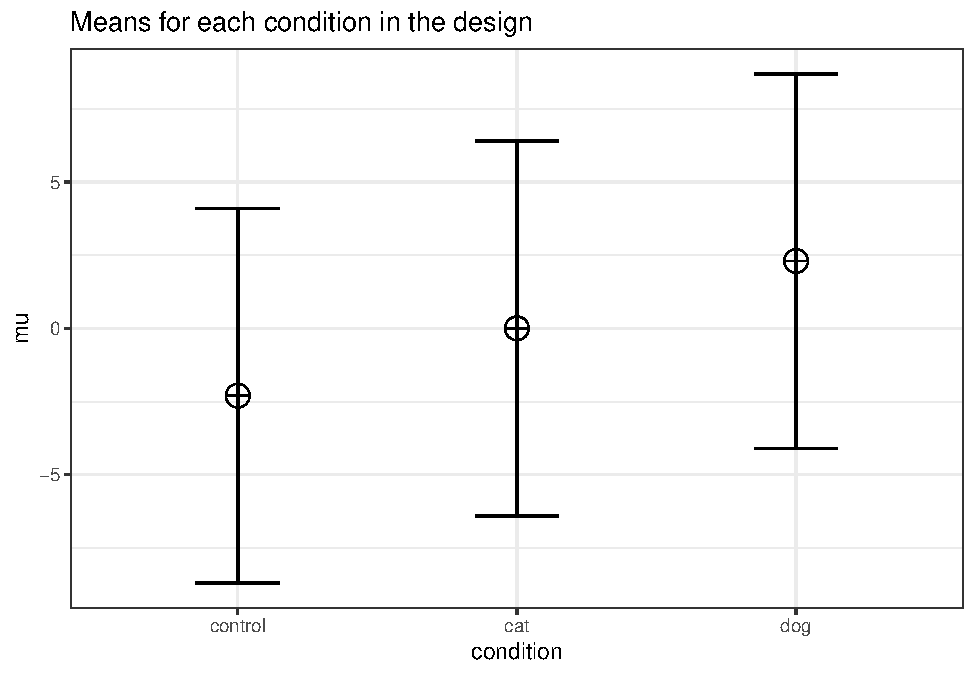
\includegraphics{SuperpowerValidation_files/figure-latex/unnamed-chunk-41-1.pdf}

\begin{Shaded}
\begin{Highlighting}[]
\NormalTok{simulation\_result }\OtherTok{\textless{}{-}} \FunctionTok{ANOVA\_power}\NormalTok{(design\_result,}
                                 \AttributeTok{alpha\_level =}\NormalTok{ alpha\_level,}
                                 \AttributeTok{nsims =}\NormalTok{ nsims,}
                                 \AttributeTok{verbose =} \ConstantTok{FALSE}\NormalTok{)}
\end{Highlighting}
\end{Shaded}

\begin{table}[!h]

\caption{\label{tab:unnamed-chunk-43}Simulated ANOVA Result}
\centering
\begin{tabular}[t]{l|r|r}
\hline
  & power & effect\_size\\
\hline
anova\_condition & 89.64 & 0.0549452\\
\hline
\end{tabular}
\end{table}

\begin{Shaded}
\begin{Highlighting}[]
\NormalTok{exact\_result }\OtherTok{\textless{}{-}} \FunctionTok{ANOVA\_exact}\NormalTok{(design\_result,}
                            \AttributeTok{alpha\_level =}\NormalTok{ alpha\_level,}
                            \AttributeTok{verbose =} \ConstantTok{FALSE}\NormalTok{)}
\end{Highlighting}
\end{Shaded}

\begin{table}[!h]

\caption{\label{tab:unnamed-chunk-45}Exact ANOVA Result}
\centering
\begin{tabular}[t]{l|r|r|r|r}
\hline
  & power & partial\_eta\_squared & cohen\_f & non\_centrality\\
\hline
condition & 90.00714 & 0.0508742 & 0.2315192 & 10.61302\\
\hline
\end{tabular}
\end{table}

The simulation confirms that for the \emph{F}-test for the ANOVA we have 90\% power. This is also what g*power tells us what would happen based on a post-hoc power analysis with an \emph{f} of 0.2303587, 2 groups, 200 participants in total (100 in each between subject condition), and an alpha of 5\%.

\includegraphics{screenshots/gpower_8.png}

If we return to our expected means, how many participants do we need for sufficient power? Given the expected difference and standard deviation, d = 0.34375, and \emph{f} = 0.171875. We can perform an a priori power analysis for this simple case, which tells us we need 179 participants in each group (we can't split people in parts, and thus always round a power analysis upward), or 358 in total.

\begin{Shaded}
\begin{Highlighting}[]
\NormalTok{K }\OtherTok{\textless{}{-}} \DecValTok{2}
\NormalTok{power }\OtherTok{\textless{}{-}} \FloatTok{0.9}
\NormalTok{f }\OtherTok{\textless{}{-}} \FloatTok{0.171875}
\FunctionTok{pwr.anova.test}\NormalTok{(}\AttributeTok{power =}\NormalTok{ power,}
               \AttributeTok{k =}\NormalTok{ K,}
               \AttributeTok{f =}\NormalTok{ f,}
               \AttributeTok{sig.level =}\NormalTok{ alpha\_level)}
\end{Highlighting}
\end{Shaded}

\begin{verbatim}
## 
##      Balanced one-way analysis of variance power calculation 
## 
##               k = 2
##               n = 178.8104
##               f = 0.171875
##       sig.level = 0.05
##           power = 0.9
## 
## NOTE: n is number in each group
\end{verbatim}

If we re-run the simulation with this sample size, we indeed have 90\% power.

\begin{Shaded}
\begin{Highlighting}[]
\NormalTok{string }\OtherTok{\textless{}{-}} \StringTok{"2b"}
\NormalTok{n }\OtherTok{\textless{}{-}} \DecValTok{179}
\NormalTok{mu }\OtherTok{\textless{}{-}} \FunctionTok{c}\NormalTok{(}\DecValTok{24}\NormalTok{, }\FloatTok{26.2}\NormalTok{)}
\CommentTok{\# Enter means in the order that matches the labels below.}
\CommentTok{\# In this case, control, pet.}
\NormalTok{sd }\OtherTok{\textless{}{-}} \FloatTok{6.4}
\NormalTok{labelnames }\OtherTok{\textless{}{-}} \FunctionTok{c}\NormalTok{(}\StringTok{"condition"}\NormalTok{, }\StringTok{"control"}\NormalTok{, }\StringTok{"pet"}\NormalTok{) }\CommentTok{\#}
\CommentTok{\# the label names should be in the order of the means specified above.}
\NormalTok{design\_result }\OtherTok{\textless{}{-}} \FunctionTok{ANOVA\_design}\NormalTok{(}
\AttributeTok{design =}\NormalTok{ string,}
\AttributeTok{n =}\NormalTok{ n,}
\AttributeTok{mu =}\NormalTok{ mu,}
\AttributeTok{sd =}\NormalTok{ sd,}
\AttributeTok{labelnames =}\NormalTok{ labelnames}
\NormalTok{)}
\end{Highlighting}
\end{Shaded}

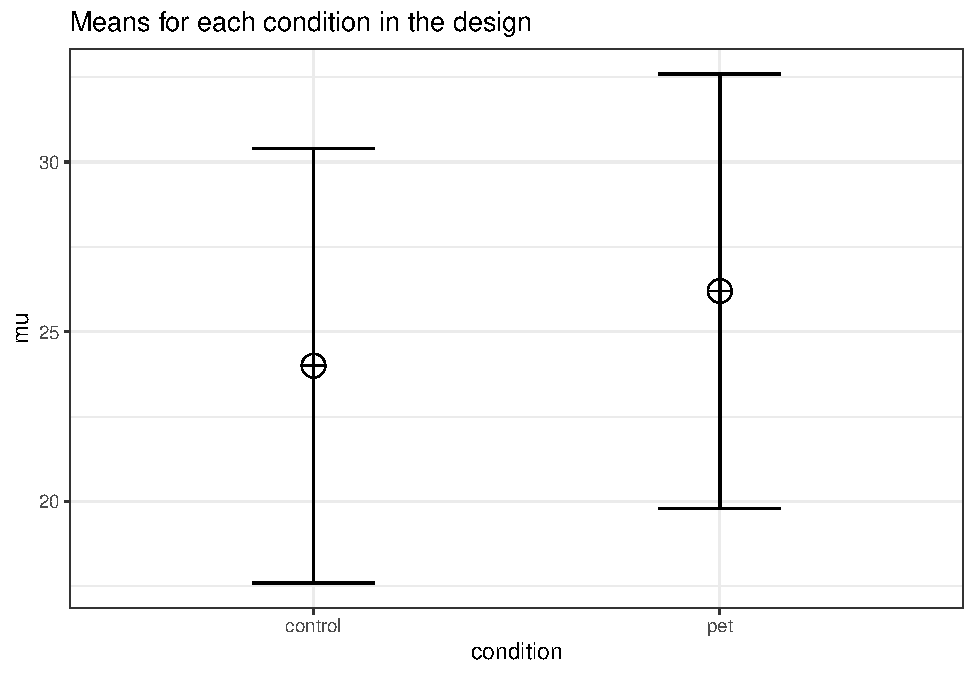
\includegraphics{SuperpowerValidation_files/figure-latex/unnamed-chunk-47-1.pdf}

\begin{Shaded}
\begin{Highlighting}[]
\NormalTok{alpha\_level }\OtherTok{\textless{}{-}} \FloatTok{0.05}
\end{Highlighting}
\end{Shaded}

\begin{Shaded}
\begin{Highlighting}[]
\NormalTok{simulation\_result }\OtherTok{\textless{}{-}} \FunctionTok{ANOVA\_power}\NormalTok{(design\_result,}
                                 \AttributeTok{alpha\_level =}\NormalTok{ alpha\_level,}
                                 \AttributeTok{nsims =}\NormalTok{ nsims,}
                                 \AttributeTok{verbose =} \ConstantTok{FALSE}\NormalTok{)}
\end{Highlighting}
\end{Shaded}

\begin{table}[!h]

\caption{\label{tab:unnamed-chunk-49}Simulated ANOVA Result}
\centering
\begin{tabular}[t]{l|r|r}
\hline
  & power & effect\_size\\
\hline
anova\_condition & 89.99 & 0.0315309\\
\hline
\end{tabular}
\end{table}

\begin{Shaded}
\begin{Highlighting}[]
\NormalTok{exact\_result }\OtherTok{\textless{}{-}} \FunctionTok{ANOVA\_exact}\NormalTok{(design\_result,}
                            \AttributeTok{alpha\_level =}\NormalTok{ alpha\_level,}
                            \AttributeTok{verbose =} \ConstantTok{FALSE}\NormalTok{)}
\end{Highlighting}
\end{Shaded}

\begin{table}[!h]

\caption{\label{tab:unnamed-chunk-51}Exact ANOVA Result}
\centering
\begin{tabular}[t]{l|r|r|r|r}
\hline
  & power & partial\_eta\_squared & cohen\_f & non\_centrality\\
\hline
condition & 90.03028 & 0.0288499 & 0.1723571 & 10.57568\\
\hline
\end{tabular}
\end{table}

We stored the result from the power analysis in an object. This allows us to request plots (which are not printed automatically) showing the \emph{p}-value distribution. If we request \texttt{simulation\_result\$plot1} we get the \emph{p}-value distribution for the ANOVA:

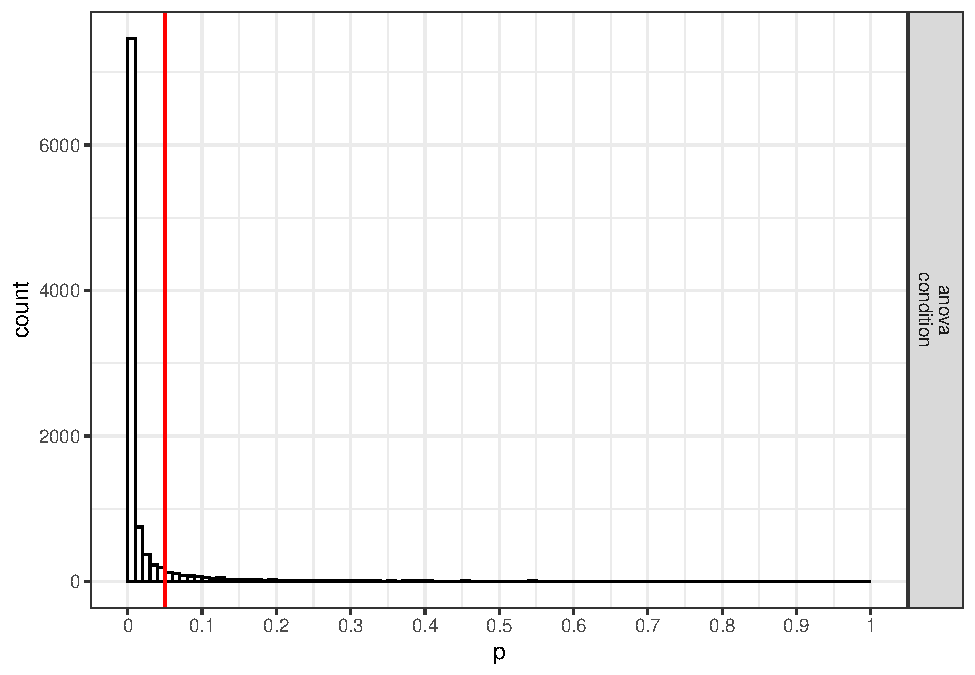
\includegraphics{SuperpowerValidation_files/figure-latex/unnamed-chunk-52-1.pdf}

If we request \texttt{simulation\_result\$plot2} we get the \emph{p}-value distribution for the paired comparisons (in this case only one):

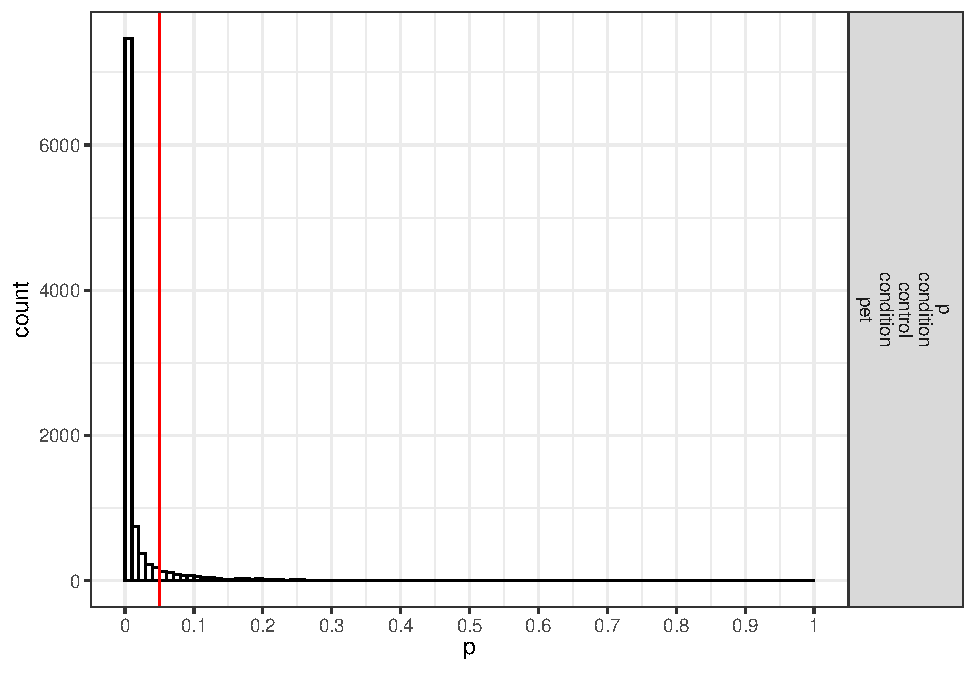
\includegraphics{SuperpowerValidation_files/figure-latex/unnamed-chunk-53-1.pdf}
\newpage
\#\# Part 2

\hypertarget{three-conditions}{%
\subsection{Three conditions}\label{three-conditions}}

Imagine we aim to design a study to test the hypothesis that giving people a pet to take care of will increase their life satisfaction. We have a control condition, a `cat' pet condition, and a `dog' pet condition. We can simulate a One-Way ANOVA with a specified alpha, sample size, and effect size, to see the statistical power we would have for the ANOVA and the follow-up comparisons. We expect all pets to increase life-satisfaction compared to the control condition. Obviously, we also expect the people who are in the `dog' pet condition to have even greater life-satisfaction than people in the `cat' pet condition. Based on work by Pavot and Diener (1993) we believe that we can expect responses on the life-satifaction scale to have a mean of approximately 24 in our population, with a standard deviation of 6.4. We expect having a pet increases life satisfaction with approximately 2.2 scale points for participants who get a cat, and 2.6 scale points for participants who get a dog. We initially consider collecting data from 150 participants in total, with 50 participants in each condition. But before we proceed with the data collection, we examine the statistical power our design would have to detect the differences we predict.

\begin{Shaded}
\begin{Highlighting}[]
\NormalTok{string }\OtherTok{\textless{}{-}} \StringTok{"3b"}
\NormalTok{n }\OtherTok{\textless{}{-}} \DecValTok{50}
\CommentTok{\# We are thinking of running 50 peope in each condition}
\NormalTok{mu }\OtherTok{\textless{}{-}} \FunctionTok{c}\NormalTok{(}\DecValTok{24}\NormalTok{, }\FloatTok{26.2}\NormalTok{, }\FloatTok{26.6}\NormalTok{)}
\CommentTok{\# Enter means in the order that matches the labels below.}
\CommentTok{\# In this case, control, cat, dog.}
\NormalTok{sd }\OtherTok{\textless{}{-}} \FloatTok{6.4}
\NormalTok{labelnames }\OtherTok{\textless{}{-}} \FunctionTok{c}\NormalTok{(}\StringTok{"condition"}\NormalTok{, }\StringTok{"control"}\NormalTok{, }\StringTok{"cat"}\NormalTok{, }\StringTok{"dog"}\NormalTok{) }\CommentTok{\#}
\CommentTok{\# the label names should be in the order of the means specified above.}
\NormalTok{design\_result }\OtherTok{\textless{}{-}} \FunctionTok{ANOVA\_design}\NormalTok{(}
\AttributeTok{design =}\NormalTok{ string,}
\AttributeTok{n =}\NormalTok{ n,}
\AttributeTok{mu =}\NormalTok{ mu,}
\AttributeTok{sd =}\NormalTok{ sd,}
\AttributeTok{labelnames =}\NormalTok{ labelnames}
\NormalTok{)}
\end{Highlighting}
\end{Shaded}

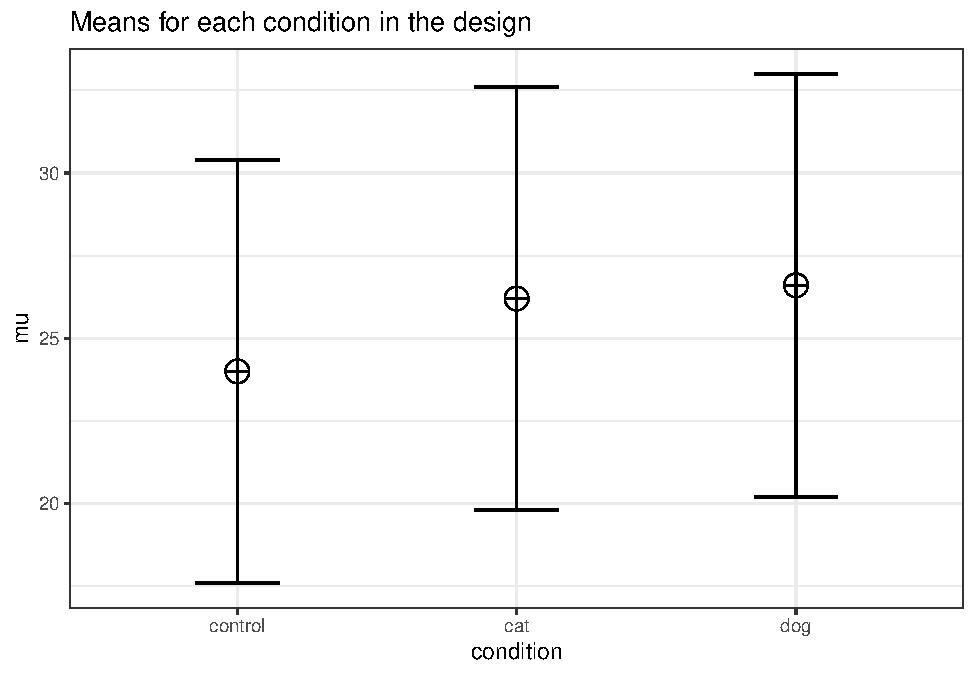
\includegraphics{SuperpowerValidation_files/figure-latex/unnamed-chunk-54-1.pdf}

\begin{Shaded}
\begin{Highlighting}[]
\NormalTok{alpha\_level }\OtherTok{\textless{}{-}} \FloatTok{0.05}
\end{Highlighting}
\end{Shaded}

\begin{Shaded}
\begin{Highlighting}[]
\CommentTok{\# You should think carefully about how to justify your alpha level.}
\CommentTok{\# We will give some examples later, but for now, use 0.05.}
\NormalTok{simulation\_result }\OtherTok{\textless{}{-}} \FunctionTok{ANOVA\_power}\NormalTok{(design\_result,}
                                 \AttributeTok{alpha\_level =}\NormalTok{ alpha\_level,}
                                 \AttributeTok{nsims =}\NormalTok{ nsims,}
                                 \AttributeTok{verbose =} \ConstantTok{FALSE}\NormalTok{)}
\end{Highlighting}
\end{Shaded}

\begin{table}[!h]

\caption{\label{tab:unnamed-chunk-56}Simulated ANOVA Result}
\centering
\begin{tabular}[t]{l|r|r}
\hline
  & power & effect\_size\\
\hline
anova\_condition & 48.22 & 0.0439651\\
\hline
\end{tabular}
\end{table}

\begin{Shaded}
\begin{Highlighting}[]
\NormalTok{exact\_result }\OtherTok{\textless{}{-}} \FunctionTok{ANOVA\_exact}\NormalTok{(design\_result,}
                            \AttributeTok{alpha\_level =}\NormalTok{ alpha\_level,}
                            \AttributeTok{verbose =} \ConstantTok{FALSE}\NormalTok{)}
\end{Highlighting}
\end{Shaded}

\begin{table}[!h]

\caption{\label{tab:unnamed-chunk-58}Exact ANOVA Result}
\centering
\begin{tabular}[t]{l|r|r|r|r}
\hline
  & power & partial\_eta\_squared & cohen\_f & non\_centrality\\
\hline
condition & 47.69468 & 0.0315259 & 0.180422 & 4.785156\\
\hline
\end{tabular}
\end{table}

The result shows that you would have quite low power with 50 participants, both for the overall ANOVA (just around 50\% power), as for the follow up comparisons (approximately 40\% power for the control vs cat condition, around 50\% for the control vs dogs condition, and really low power (around 6\%, just above the Type 1 error rate of 5\%) for the expected difference between cats and dogs.

\hypertarget{power-for-simple-effects}{%
\subsection{Power for simple effects}\label{power-for-simple-effects}}

We are typically not just interested in the ANOVA, but also in follow up comparisons. In this case, we would perform a \emph{t}-test comparing the control condition against the cat and dog condition, and we would compare the cat and dog conditions against each other, in independent \emph{t}-tests.

For our example, Cohen's d (the standardized mean difference) is 2.2/6.4, or d = 0.34375 for the difference between the control condition and cats, 2.6/6.4 of d = 0.40625 for the difference between the control condition and dogs, and 0.4/6.4 or d = 0.0625 for the difference between cats and dogs as pets.

We can easily compute the expected power for these simple comparisons using the \texttt{pwr} package.

\begin{Shaded}
\begin{Highlighting}[]
\FunctionTok{pwr.t.test}\NormalTok{(}
  \AttributeTok{d =} \FloatTok{2.2} \SpecialCharTok{/} \FloatTok{6.4}\NormalTok{,}
  \AttributeTok{n =} \DecValTok{50}\NormalTok{,}
  \AttributeTok{sig.level =} \FloatTok{0.05}\NormalTok{,}
  \AttributeTok{type =} \StringTok{"two.sample"}\NormalTok{,}
  \AttributeTok{alternative =} \StringTok{"two.sided"}
\NormalTok{  )}\SpecialCharTok{$}\NormalTok{power}
\end{Highlighting}
\end{Shaded}

\begin{verbatim}
## [1] 0.3983064
\end{verbatim}

\begin{Shaded}
\begin{Highlighting}[]
  \FunctionTok{pwr.t.test}\NormalTok{(}
  \AttributeTok{d =} \FloatTok{2.6} \SpecialCharTok{/} \FloatTok{6.4}\NormalTok{,}
  \AttributeTok{n =} \DecValTok{50}\NormalTok{,}
  \AttributeTok{sig.level =} \FloatTok{0.05}\NormalTok{,}
  \AttributeTok{type =} \StringTok{"two.sample"}\NormalTok{,}
  \AttributeTok{alternative =} \StringTok{"two.sided"}
\NormalTok{  )}\SpecialCharTok{$}\NormalTok{power}
\end{Highlighting}
\end{Shaded}

\begin{verbatim}
## [1] 0.5205162
\end{verbatim}

\begin{Shaded}
\begin{Highlighting}[]
  \FunctionTok{pwr.t.test}\NormalTok{(}
  \AttributeTok{d =} \FloatTok{0.4} \SpecialCharTok{/} \FloatTok{6.4}\NormalTok{,}
  \AttributeTok{n =} \DecValTok{50}\NormalTok{,}
  \AttributeTok{sig.level =} \FloatTok{0.05}\NormalTok{,}
  \AttributeTok{type =} \StringTok{"two.sample"}\NormalTok{,}
  \AttributeTok{alternative =} \StringTok{"two.sided"}
\NormalTok{  )}\SpecialCharTok{$}\NormalTok{power}
\end{Highlighting}
\end{Shaded}

\begin{verbatim}
## [1] 0.06104044
\end{verbatim}

This analysis tells us that running the study with 50 participants in each condition is more likely to \emph{not} yield a significant test result, even if our expected pattern of differences is true, than that we will observe a \emph{p}-value smaller than our alpha level. This is not optimal.

Let's mathematically explore which pattern of means we would need to expect to have 90\% power for the ANOVA with 50 participants in each group. We can use the \texttt{pwr} package in R to compute a sensitivity analysis that tells us the effect size, in Cohen's \emph{f}, that we are able to detect with 3 groups and 50 partiicpants in each group, in order to achive 90\% power with an alpha level of 5\%.

\begin{Shaded}
\begin{Highlighting}[]
\NormalTok{K }\OtherTok{\textless{}{-}} \DecValTok{3}
\NormalTok{n }\OtherTok{\textless{}{-}} \DecValTok{50}
\NormalTok{sd }\OtherTok{\textless{}{-}} \FloatTok{6.4}
\NormalTok{r }\OtherTok{\textless{}{-}} \DecValTok{0}
\CommentTok{\#Calculate f when running simulation}
\NormalTok{f }\OtherTok{\textless{}{-}} \FunctionTok{pwr.anova.test}\NormalTok{(}\AttributeTok{n =}\NormalTok{ n,}
                    \AttributeTok{k =}\NormalTok{ K,}
                    \AttributeTok{power =} \FloatTok{0.9}\NormalTok{,}
                    \AttributeTok{sig.level =}\NormalTok{ alpha\_level)}\SpecialCharTok{$}\NormalTok{f}
\NormalTok{f}
\end{Highlighting}
\end{Shaded}

\begin{verbatim}
## [1] 0.2934417
\end{verbatim}

This sensitivity analysis shows we have 90\% power in our planned design to detect effects of Cohen's \emph{f} of 0.2934417. Benchmarks by \citet{cohen1988spa} for small, medium, and large Cohen's \emph{f} values are 0.1, 0.25, and 0.4, which correspond to eta-squared values of small (.0099), medium (.0588), and large (.1379), in line with d = .2, .5, or .8. So, at least based on these benchmarks, we have 90\% power to detect effects that are somewhat sizeable.

\begin{Shaded}
\begin{Highlighting}[]
\NormalTok{f2 }\OtherTok{\textless{}{-}}\NormalTok{ f}\SpecialCharTok{\^{}}\DecValTok{2}
\NormalTok{ES }\OtherTok{\textless{}{-}}\NormalTok{ f2 }\SpecialCharTok{/}\NormalTok{ (f2 }\SpecialCharTok{+} \DecValTok{1}\NormalTok{)}
\NormalTok{ES}
\end{Highlighting}
\end{Shaded}

\begin{verbatim}
## [1] 0.07928127
\end{verbatim}

Expressed in eta-squared, we can detect values of eta-squared = 0.0793 or larger.

\begin{Shaded}
\begin{Highlighting}[]
\NormalTok{mu }\OtherTok{\textless{}{-}} \FunctionTok{mu\_from\_ES}\NormalTok{(}\AttributeTok{K =}\NormalTok{ K, }\AttributeTok{ES =}\NormalTok{ ES)}
\NormalTok{mu }\OtherTok{\textless{}{-}}\NormalTok{ mu }\SpecialCharTok{*}\NormalTok{ sd}
\NormalTok{mu}
\end{Highlighting}
\end{Shaded}

\begin{verbatim}
## [1] -2.300104  0.000000  2.300104
\end{verbatim}

We can compute a pattern of means, given a standard deviation of 6.4, that would give us an effect size of f = 0.2934, or eta-squared of 0.0793. We should be able to accomplish this if the means are -2.300104, 0.000000, and 2.300104. We can use these values to confirm the ANOVA has 90\% power.

\begin{Shaded}
\begin{Highlighting}[]
\NormalTok{design\_result }\OtherTok{\textless{}{-}} \FunctionTok{ANOVA\_design}\NormalTok{(}
  \AttributeTok{design =}\NormalTok{ string,}
  \AttributeTok{n =}\NormalTok{ n,}
  \AttributeTok{mu =}\NormalTok{ mu,}
  \AttributeTok{sd =}\NormalTok{ sd,}
  \AttributeTok{labelnames =}\NormalTok{ labelnames}
\NormalTok{  )}
\end{Highlighting}
\end{Shaded}

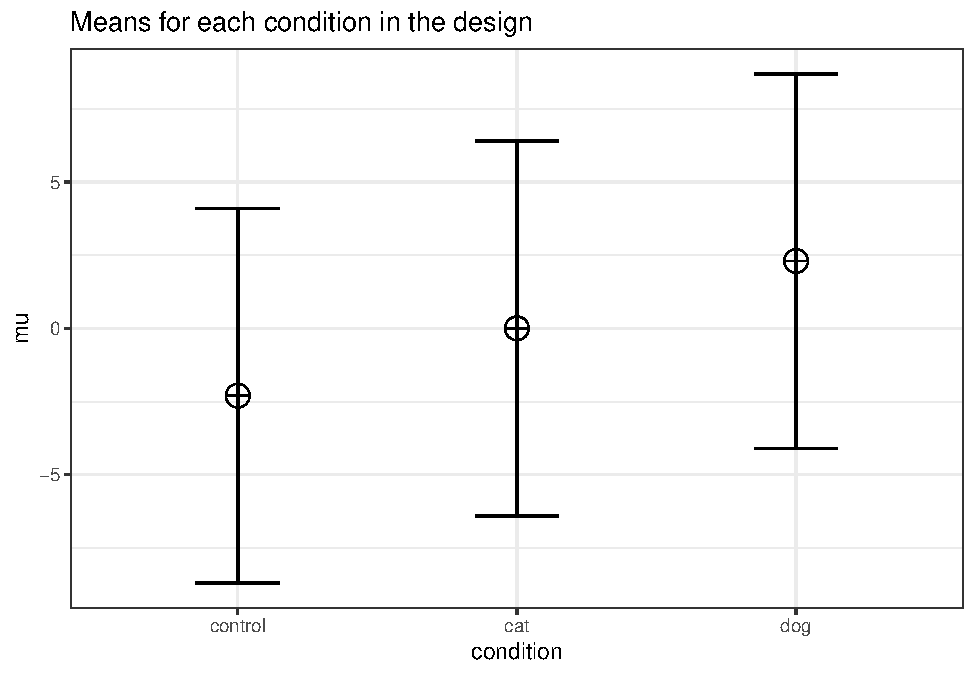
\includegraphics{SuperpowerValidation_files/figure-latex/unnamed-chunk-63-1.pdf}

\begin{Shaded}
\begin{Highlighting}[]
\NormalTok{simulation\_result }\OtherTok{\textless{}{-}} \FunctionTok{ANOVA\_power}\NormalTok{(design\_result,}
                                 \AttributeTok{alpha\_level =}\NormalTok{ alpha\_level,}
                                 \AttributeTok{nsims =}\NormalTok{ nsims,}
                                 \AttributeTok{verbose =} \ConstantTok{FALSE}\NormalTok{)}
\end{Highlighting}
\end{Shaded}

\begin{table}[!h]

\caption{\label{tab:unnamed-chunk-65}Simulated ANOVA Result}
\centering
\begin{tabular}[t]{l|r|r}
\hline
  & power & effect\_size\\
\hline
anova\_condition & 90.01 & 0.0903282\\
\hline
\end{tabular}
\end{table}

\begin{Shaded}
\begin{Highlighting}[]
\NormalTok{exact\_result }\OtherTok{\textless{}{-}} \FunctionTok{ANOVA\_exact}\NormalTok{(design\_result,}
                            \AttributeTok{alpha\_level =}\NormalTok{ alpha\_level,}
                            \AttributeTok{verbose =} \ConstantTok{FALSE}\NormalTok{)}
\end{Highlighting}
\end{Shaded}

\begin{table}[!h]

\caption{\label{tab:unnamed-chunk-67}Exact ANOVA Result}
\centering
\begin{tabular}[t]{l|r|r|r|r}
\hline
  & power & partial\_eta\_squared & cohen\_f & non\_centrality\\
\hline
condition & 90.00112 & 0.0807686 & 0.2964209 & 12.9162\\
\hline
\end{tabular}
\end{table}

The simulation confirms that for the \emph{F}-test for the ANOVA we have 90\% power. This is also what g*power tells us what would happen based on a post-hoc power analysis with an f of 0.2934417, 3 groups, 150 participants in total (50 in each between subject condition), and an alpha of 5\%.

\includegraphics{screenshots/gpower_7.png}

We can also compute the power for the ANOVA and simple effects in \texttt{R} with the \texttt{pwr} package. The calculated effect sizes and power match those from the simulation.

\begin{Shaded}
\begin{Highlighting}[]
\NormalTok{K }\OtherTok{\textless{}{-}} \DecValTok{3}
\NormalTok{n }\OtherTok{\textless{}{-}} \DecValTok{50}
\NormalTok{sd }\OtherTok{\textless{}{-}} \FloatTok{6.4}
\NormalTok{f }\OtherTok{\textless{}{-}} \FloatTok{0.2934417}
\FunctionTok{pwr.anova.test}\NormalTok{(}
\AttributeTok{n =}\NormalTok{ n,}
\AttributeTok{k =}\NormalTok{ K,}
\AttributeTok{f =}\NormalTok{ f,}
\AttributeTok{sig.level =}\NormalTok{ alpha\_level}
\NormalTok{)}\SpecialCharTok{$}\NormalTok{power}
\end{Highlighting}
\end{Shaded}

\begin{verbatim}
## [1] 0.9000112
\end{verbatim}

\begin{Shaded}
\begin{Highlighting}[]
\NormalTok{d }\OtherTok{\textless{}{-}} \FloatTok{2.300104} \SpecialCharTok{/} \FloatTok{6.4}
\NormalTok{d}
\end{Highlighting}
\end{Shaded}

\begin{verbatim}
## [1] 0.3593912
\end{verbatim}

\begin{Shaded}
\begin{Highlighting}[]
\FunctionTok{pwr.t.test}\NormalTok{(}
\AttributeTok{d =} \FloatTok{2.300104} \SpecialCharTok{/} \FloatTok{6.4}\NormalTok{,}
\AttributeTok{n =} \DecValTok{50}\NormalTok{,}
\AttributeTok{sig.level =} \FloatTok{0.05}\NormalTok{,}
\AttributeTok{type =} \StringTok{"two.sample"}\NormalTok{,}
\AttributeTok{alternative =} \StringTok{"two.sided"}
\NormalTok{)}\SpecialCharTok{$}\NormalTok{power}
\end{Highlighting}
\end{Shaded}

\begin{verbatim}
## [1] 0.4284243
\end{verbatim}

\begin{Shaded}
\begin{Highlighting}[]
\NormalTok{d }\OtherTok{\textless{}{-}} \DecValTok{2} \SpecialCharTok{*} \FloatTok{2.300104} \SpecialCharTok{/} \FloatTok{6.4}
\NormalTok{d}
\end{Highlighting}
\end{Shaded}

\begin{verbatim}
## [1] 0.7187825
\end{verbatim}

\begin{Shaded}
\begin{Highlighting}[]
\FunctionTok{pwr.t.test}\NormalTok{(}
\AttributeTok{d =}\NormalTok{ d,}
\AttributeTok{n =} \DecValTok{50}\NormalTok{,}
\AttributeTok{sig.level =} \FloatTok{0.05}\NormalTok{,}
\AttributeTok{type =} \StringTok{"two.sample"}\NormalTok{,}
\AttributeTok{alternative =} \StringTok{"two.sided"}
\NormalTok{)}\SpecialCharTok{$}\NormalTok{power}
\end{Highlighting}
\end{Shaded}

\begin{verbatim}
## [1] 0.9450353
\end{verbatim}

We can also compare the results against the analytic solution by Aberson (2019).

First, load the function for a 3-way ANOVA from the \texttt{pwr2ppl} package.

Then we use the function to calculate power.

\begin{Shaded}
\begin{Highlighting}[]
\CommentTok{\#Initial example, low power}
\FunctionTok{anova1f\_3}\NormalTok{(}
\AttributeTok{m1 =} \DecValTok{24}\NormalTok{,}
\AttributeTok{m2 =} \FloatTok{26.2}\NormalTok{,}
\AttributeTok{m3 =} \FloatTok{26.6}\NormalTok{,}
\AttributeTok{s1 =} \FloatTok{6.4}\NormalTok{,}
\AttributeTok{s2 =} \FloatTok{6.4}\NormalTok{,}
\AttributeTok{s3 =} \FloatTok{6.4}\NormalTok{,}
\AttributeTok{n1 =} \DecValTok{50}\NormalTok{,}
\AttributeTok{n2 =} \DecValTok{50}\NormalTok{,}
\AttributeTok{n3 =} \DecValTok{50}\NormalTok{,}
\AttributeTok{alpha =}\NormalTok{ .}\DecValTok{05}
\NormalTok{)}
\end{Highlighting}
\end{Shaded}

\begin{verbatim}
## Sample size overall = 150
\end{verbatim}

\begin{verbatim}
## Power  = 0.4769 for eta-squared = 0.0315
\end{verbatim}

\begin{Shaded}
\begin{Highlighting}[]
\CommentTok{\#From: Aberson, Christopher L.}
\CommentTok{\#   Applied Power Analysis for the Behavioral Sciences, 2nd Edition.}
\CommentTok{\# $Power [1] 0.4769468}
\CommentTok{\#Later example, based on larger mean difference}
\FunctionTok{anova1f\_3}\NormalTok{(}
\AttributeTok{m1 =} \SpecialCharTok{{-}}\FloatTok{2.300104}\NormalTok{,}
\AttributeTok{m2 =} \DecValTok{0}\NormalTok{,}
\AttributeTok{m3 =} \FloatTok{2.300104}\NormalTok{,}
\AttributeTok{s1 =} \FloatTok{6.4}\NormalTok{,}
\AttributeTok{s2 =} \FloatTok{6.4}\NormalTok{,}
\AttributeTok{s3 =} \FloatTok{6.4}\NormalTok{,}
\AttributeTok{n1 =} \DecValTok{50}\NormalTok{,}
\AttributeTok{n2 =} \DecValTok{50}\NormalTok{,}
\AttributeTok{n3 =} \DecValTok{50}\NormalTok{,}
\AttributeTok{alpha =}\NormalTok{ .}\DecValTok{05}
\NormalTok{)}
\end{Highlighting}
\end{Shaded}

\begin{verbatim}
## Sample size overall = 150
\end{verbatim}

\begin{verbatim}
## Power  = 0.9 for eta-squared = 0.0808
\end{verbatim}

\begin{Shaded}
\begin{Highlighting}[]
\CommentTok{\# $Power [1] 0.9000112}
\end{Highlighting}
\end{Shaded}

\newpage

\hypertarget{effect-size-estimates-for-one-way-anova}{%
\section{Effect Size Estimates for One-Way ANOVA}\label{effect-size-estimates-for-one-way-anova}}

Using the formulas below, we can calculate the means for a one-way ANOVA. Using the formula from \citet{albers2018power}, we can determine the means that should yield a specified effect sizes (expressed in Cohen's \emph{f}).

Eta-squared (idential to partial eta-squared for one-way ANOVA's) has benchmarks of .0099, .0588, and .1379 for small, medium, and large effect sizes \citep{cohen1988spa}.

\hypertarget{three-conditions-small-effect-size}{%
\subsection{Three conditions, small effect size}\label{three-conditions-small-effect-size}}

We can simulate a one-factor anova, setting means to achieve a certain effect size. Eta-squared is biased. Thus, the eta-squared we calculate based on the observed data overestimates the population effect size. This bias is largest for smaller sample sizes. Thus, to test whether the simulation yields the expected effect size, we use extremele large sample sizes in each between subject condition (n = 5000). This simulation should yield a small effect size (0.099)

\begin{Shaded}
\begin{Highlighting}[]
\NormalTok{K }\OtherTok{\textless{}{-}} \DecValTok{3}
\NormalTok{ES }\OtherTok{\textless{}{-}}\NormalTok{ .}\DecValTok{0099}
\NormalTok{mu }\OtherTok{\textless{}{-}} \FunctionTok{mu\_from\_ES}\NormalTok{(}\AttributeTok{K =}\NormalTok{ K, }\AttributeTok{ES =}\NormalTok{ ES)}
\NormalTok{n }\OtherTok{\textless{}{-}} \DecValTok{5000}
\NormalTok{sd }\OtherTok{\textless{}{-}} \DecValTok{1}
\NormalTok{r }\OtherTok{\textless{}{-}} \DecValTok{0}
\NormalTok{string }\OtherTok{=} \FunctionTok{paste}\NormalTok{(K,}\StringTok{"b"}\NormalTok{,}\AttributeTok{sep =} \StringTok{""}\NormalTok{)}
\end{Highlighting}
\end{Shaded}

\begin{Shaded}
\begin{Highlighting}[]
\NormalTok{design\_result }\OtherTok{\textless{}{-}} \FunctionTok{ANOVA\_design}\NormalTok{(}
  \AttributeTok{design =}\NormalTok{ string,}
  \AttributeTok{n =}\NormalTok{ n,}
  \AttributeTok{mu =}\NormalTok{ mu,}
  \AttributeTok{sd =}\NormalTok{ sd,}
  \AttributeTok{r =}\NormalTok{ r,}
  \AttributeTok{labelnames =} \FunctionTok{c}\NormalTok{(}\StringTok{"factor1"}\NormalTok{, }\StringTok{"level1"}\NormalTok{, }\StringTok{"level2"}\NormalTok{, }\StringTok{"level3"}\NormalTok{)}
\NormalTok{  )}
\end{Highlighting}
\end{Shaded}

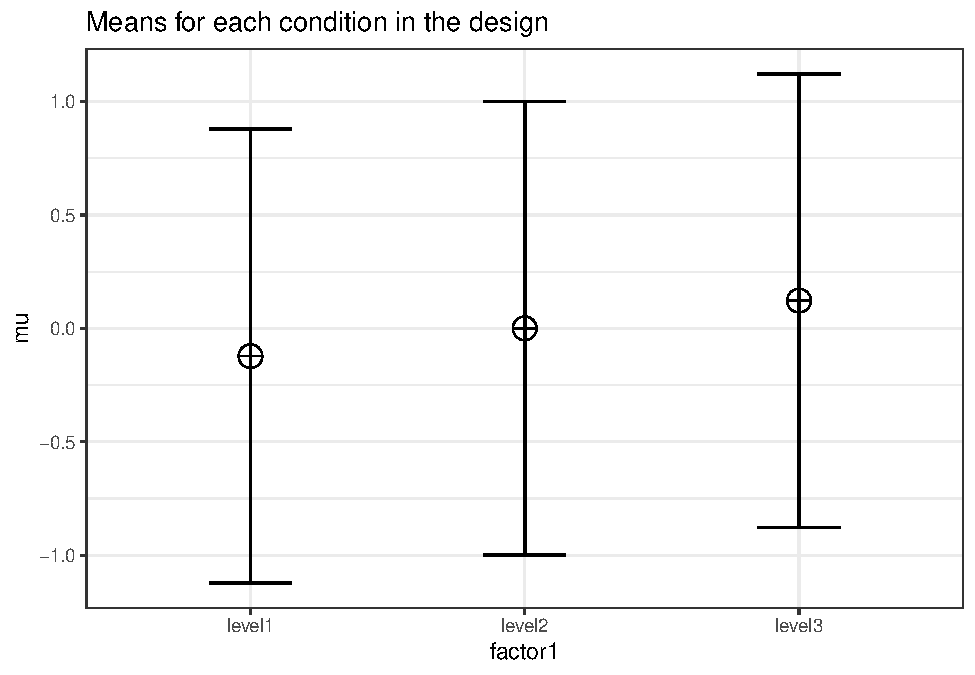
\includegraphics{SuperpowerValidation_files/figure-latex/unnamed-chunk-70-1.pdf}

\begin{Shaded}
\begin{Highlighting}[]
\NormalTok{simulation\_result }\OtherTok{\textless{}{-}} \FunctionTok{ANOVA\_power}\NormalTok{(design\_result,}
                                 \AttributeTok{alpha\_level =}\NormalTok{ alpha\_level,}
                                 \AttributeTok{nsims =}\NormalTok{ nsims,}
                                 \AttributeTok{verbose =} \ConstantTok{FALSE}\NormalTok{)}
\end{Highlighting}
\end{Shaded}

\begin{table}[!h]

\caption{\label{tab:unnamed-chunk-72}Simulated ANOVA Result}
\centering
\begin{tabular}[t]{l|r|r}
\hline
  & power & effect\_size\\
\hline
anova\_factor1 & 100 & 0.0100136\\
\hline
\end{tabular}
\end{table}

\begin{Shaded}
\begin{Highlighting}[]
\NormalTok{exact\_result }\OtherTok{\textless{}{-}} \FunctionTok{ANOVA\_exact}\NormalTok{(design\_result,}
                            \AttributeTok{alpha\_level =}\NormalTok{ alpha\_level,}
                            \AttributeTok{verbose =} \ConstantTok{FALSE}\NormalTok{)}
\end{Highlighting}
\end{Shaded}

\begin{table}[!h]

\caption{\label{tab:unnamed-chunk-74}Exact ANOVA Result}
\centering
\begin{tabular}[t]{l|r|r|r|r}
\hline
  & power & partial\_eta\_squared & cohen\_f & non\_centrality\\
\hline
factor1 & 100 & 0.009902 & 0.100005 & 149.9848\\
\hline
\end{tabular}
\end{table}

The resulting effect size estimate from the simulation is very close to 0.0099

\hypertarget{four-conditions-medium-effect-size}{%
\subsection{Four conditions, medium effect size}\label{four-conditions-medium-effect-size}}

This simulation should yield a medium effect size (0.0588) across four independent conditions.

\begin{Shaded}
\begin{Highlighting}[]
\NormalTok{K }\OtherTok{\textless{}{-}} \DecValTok{4}
\NormalTok{ES }\OtherTok{\textless{}{-}}\NormalTok{ .}\DecValTok{0588}
\NormalTok{mu }\OtherTok{\textless{}{-}} \FunctionTok{mu\_from\_ES}\NormalTok{(}\AttributeTok{K =}\NormalTok{ K, }\AttributeTok{ES =}\NormalTok{ ES)}
\NormalTok{n }\OtherTok{\textless{}{-}} \DecValTok{5000}
\NormalTok{sd }\OtherTok{\textless{}{-}} \DecValTok{1}
\NormalTok{r }\OtherTok{\textless{}{-}} \DecValTok{0}
\NormalTok{string }\OtherTok{=} \FunctionTok{paste}\NormalTok{(K,}\StringTok{"b"}\NormalTok{,}\AttributeTok{sep =} \StringTok{""}\NormalTok{)}
\end{Highlighting}
\end{Shaded}

\begin{Shaded}
\begin{Highlighting}[]
\NormalTok{design\_result }\OtherTok{\textless{}{-}} \FunctionTok{ANOVA\_design}\NormalTok{(}
  \AttributeTok{design =}\NormalTok{ string,}
  \AttributeTok{n =}\NormalTok{ n,}
  \AttributeTok{mu =}\NormalTok{ mu,}
  \AttributeTok{sd =}\NormalTok{ sd,}
  \AttributeTok{r =}\NormalTok{ r,}
  \AttributeTok{labelnames =} \FunctionTok{c}\NormalTok{(}\StringTok{"factor1"}\NormalTok{, }\StringTok{"level1"}\NormalTok{, }\StringTok{"level2"}\NormalTok{, }\StringTok{"level3"}\NormalTok{, }\StringTok{"level4"}\NormalTok{)}
\NormalTok{  )}
\end{Highlighting}
\end{Shaded}

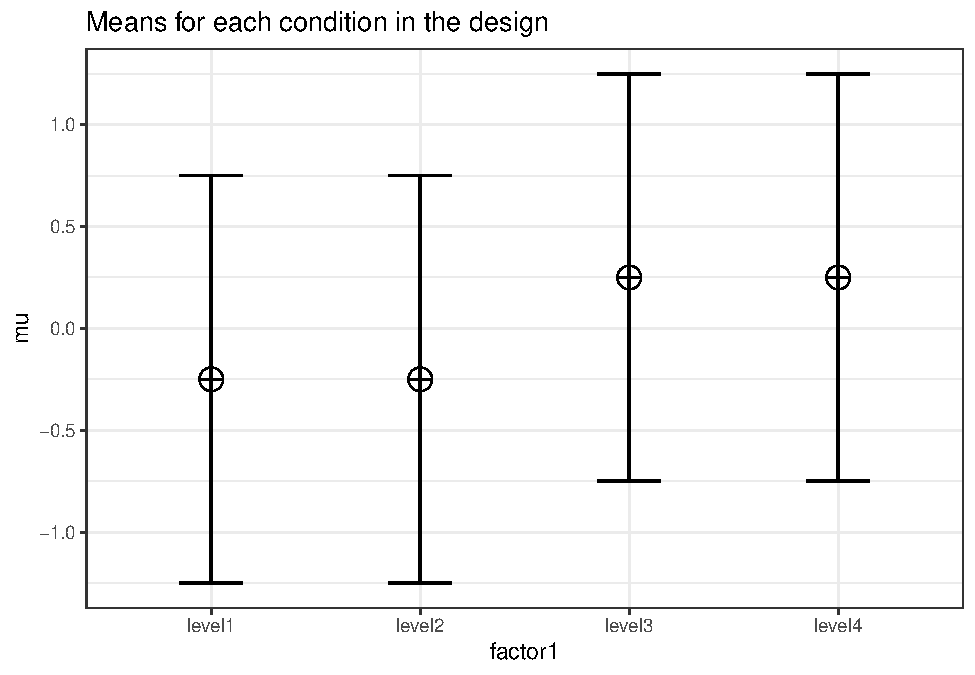
\includegraphics{SuperpowerValidation_files/figure-latex/unnamed-chunk-76-1.pdf}

\begin{Shaded}
\begin{Highlighting}[]
\NormalTok{simulation\_result }\OtherTok{\textless{}{-}} \FunctionTok{ANOVA\_power}\NormalTok{(design\_result,}
                                 \AttributeTok{alpha\_level =}\NormalTok{ alpha\_level,}
                                 \AttributeTok{nsims =}\NormalTok{ nsims,}
                                 \AttributeTok{verbose =} \ConstantTok{FALSE}\NormalTok{)}
\end{Highlighting}
\end{Shaded}

\begin{table}[!h]

\caption{\label{tab:unnamed-chunk-78}Simulated ANOVA Result}
\centering
\begin{tabular}[t]{l|r|r}
\hline
  & power & effect\_size\\
\hline
anova\_factor1 & 100 & 0.0589616\\
\hline
\end{tabular}
\end{table}

\begin{Shaded}
\begin{Highlighting}[]
\NormalTok{exact\_result }\OtherTok{\textless{}{-}} \FunctionTok{ANOVA\_exact}\NormalTok{(design\_result,}
                            \AttributeTok{alpha\_level =}\NormalTok{ alpha\_level,}
                            \AttributeTok{verbose =} \ConstantTok{FALSE}\NormalTok{)}
\end{Highlighting}
\end{Shaded}

\begin{table}[!h]

\caption{\label{tab:unnamed-chunk-80}Exact ANOVA Result}
\centering
\begin{tabular}[t]{l|r|r|r|r}
\hline
  & power & partial\_eta\_squared & cohen\_f & non\_centrality\\
\hline
factor1 & 100 & 0.0588111 & 0.2499719 & 1249.469\\
\hline
\end{tabular}
\end{table}

Results are very close to 0.0588.

\hypertarget{two-conditions-large-effect-size}{%
\subsection{Two conditions, large effect size}\label{two-conditions-large-effect-size}}

We can simulate a one-way ANOVA that should yield a large effect size (0.1379) across two conditions.

\begin{Shaded}
\begin{Highlighting}[]
\NormalTok{K }\OtherTok{\textless{}{-}} \DecValTok{2}
\NormalTok{ES }\OtherTok{\textless{}{-}}\NormalTok{ .}\DecValTok{1379}
\NormalTok{mu }\OtherTok{\textless{}{-}} \FunctionTok{mu\_from\_ES}\NormalTok{(}\AttributeTok{K =}\NormalTok{ K, }\AttributeTok{ES =}\NormalTok{ ES)}
\NormalTok{n }\OtherTok{\textless{}{-}} \DecValTok{5000}
\NormalTok{sd }\OtherTok{\textless{}{-}} \DecValTok{1}
\NormalTok{r }\OtherTok{\textless{}{-}} \DecValTok{0}
\NormalTok{string }\OtherTok{=} \FunctionTok{paste}\NormalTok{(K,}\StringTok{"b"}\NormalTok{,}\AttributeTok{sep =} \StringTok{""}\NormalTok{)}
\end{Highlighting}
\end{Shaded}

\begin{Shaded}
\begin{Highlighting}[]
\NormalTok{design\_result }\OtherTok{\textless{}{-}} \FunctionTok{ANOVA\_design}\NormalTok{(}\AttributeTok{design =}\NormalTok{ string,}
                   \AttributeTok{n =}\NormalTok{ n,}
                   \AttributeTok{mu =}\NormalTok{ mu,}
                   \AttributeTok{sd =}\NormalTok{ sd,}
                   \AttributeTok{r =}\NormalTok{ r,}
                   \AttributeTok{labelnames =} \FunctionTok{c}\NormalTok{(}\StringTok{"factor1"}\NormalTok{, }\StringTok{"level1"}\NormalTok{, }\StringTok{"level2"}\NormalTok{))}
\end{Highlighting}
\end{Shaded}

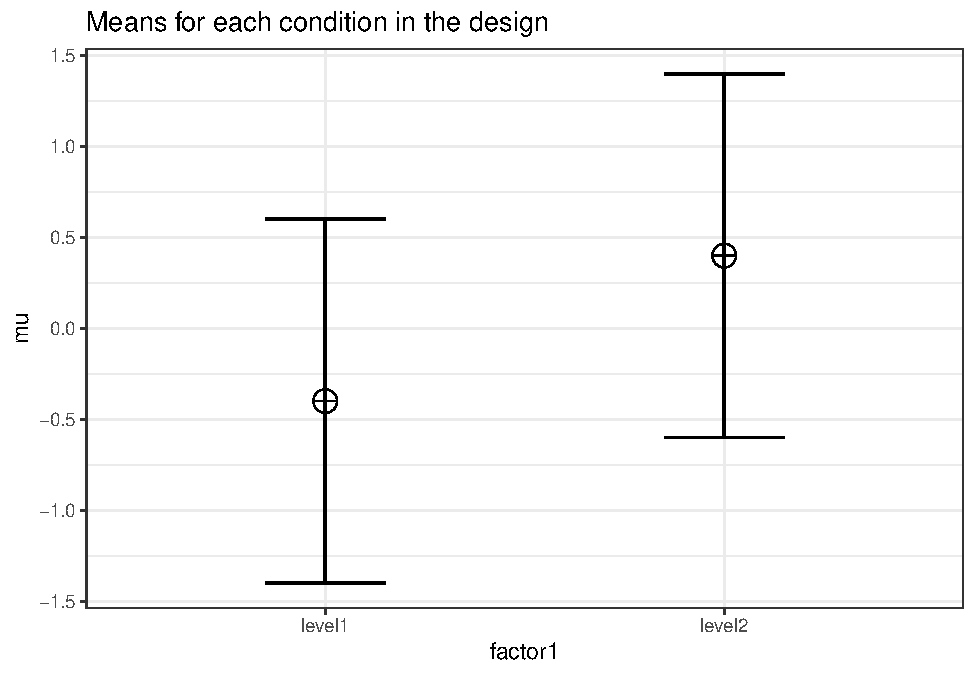
\includegraphics{SuperpowerValidation_files/figure-latex/unnamed-chunk-82-1.pdf}

\begin{Shaded}
\begin{Highlighting}[]
\NormalTok{simulation\_result }\OtherTok{\textless{}{-}} \FunctionTok{ANOVA\_power}\NormalTok{(design\_result,}
                                 \AttributeTok{alpha\_level =}\NormalTok{ alpha\_level,}
                                 \AttributeTok{nsims =}\NormalTok{ nsims,}
                                 \AttributeTok{verbose =} \ConstantTok{FALSE}\NormalTok{)}
\end{Highlighting}
\end{Shaded}

\begin{table}[!h]

\caption{\label{tab:unnamed-chunk-84}Simulated ANOVA Result}
\centering
\begin{tabular}[t]{l|r|r}
\hline
  & power & effect\_size\\
\hline
anova\_factor1 & 100 & 0.1379965\\
\hline
\end{tabular}
\end{table}

\begin{Shaded}
\begin{Highlighting}[]
\NormalTok{exact\_result }\OtherTok{\textless{}{-}} \FunctionTok{ANOVA\_exact}\NormalTok{(design\_result,}
                            \AttributeTok{alpha\_level =}\NormalTok{ alpha\_level,}
                            \AttributeTok{verbose =} \ConstantTok{FALSE}\NormalTok{)}
\end{Highlighting}
\end{Shaded}

\begin{table}[!h]

\caption{\label{tab:unnamed-chunk-86}Exact ANOVA Result}
\centering
\begin{tabular}[t]{l|r|r|r|r}
\hline
  & power & partial\_eta\_squared & cohen\_f & non\_centrality\\
\hline
factor1 & 100 & 0.1379238 & 0.3999878 & 1599.582\\
\hline
\end{tabular}
\end{table}

The results are very close to is simulation should yield a small effect size (0.1379).

\hypertarget{repeated-measures-anova}{%
\chapter{Repeated Measures ANOVA}\label{repeated-measures-anova}}

\hypertarget{part-1}{%
\section{Part 1}\label{part-1}}

In a repeated measures design multiple observations are collected from the same participants. In the simplest case, where there are two repeated observations, a repeated measures ANOVA equals a dependent or paired \emph{t}-test. The advantage of repeated measures designs is that they capitalize on the correlations between the repeated measurements. Let's first explore the impact of this correlation on the power of a repeated measures ANOVA.

\hypertarget{two-conditions-medium-effect-size}{%
\subsection{Two conditions, medium effect size}\label{two-conditions-medium-effect-size}}

To illustrate the effect of correated observations, we start by simulating data for a medium effect size for a dependent (or paired, or within-subject) \emph{t}-test. Let's first look at g*power \citet{faul2007g}. If we want to perform an a-priori power analysis, we are asked to fill in the effect size dz. As \citet{cohen1988spa} writes, ``The Z subscript is used to emphasize the fact that our raw score unit is no longer X or Y, but Z'', where Z are the difference scores of X-Y.

\includegraphics{screenshots/gpower_9.png}

Within designs can have greater power to detect differences than between designs because the values are correlated, and a within design requires less participants because each participant provides multiple observations. One difference between an independent \emph{t}-test and a dependent \emph{t}-test is that an independent \emph{t}-test has 2(n-1) degrees of freedom, while a dependent \emph{t}-test has (n-1) degrees of freedom. The sample size needed in a two-group within-design (NW) relative to the sample needed in two-group between-designs (NB), assuming normal distributions, and ignoring the difference in degrees of freedom between the two types of tests, is (from \citet{maxwell_designing_2004}, p.~561, formula 45):

\(N_{W}=\frac{N_{B}(1-\rho)}{2}\)

The division by 2 in the equation is due to the fact that in a two-condition within design every participant provides two data-points. The extent to which this reduces the sample size compared to a between-subject design depends on the correlation (\emph{r}) between the two dependent variables, as indicated by the \texttt{1-r} part of the equation. If the correlation is 0, a within-subject design needs half as many participants as a between-subject design (e.g., 64 instead 128 participants), simply because every participants provides 2 datapoints. The higher the correlation, the larger the relative benefit of within designs, and whenever the correlation is negative (up to -1) the relative benefit disappears.

Whereas in an independent \emph{t}-test the two observations are uncorrelated, in a within design the observations are correlated. This has an effect on the standard deviation of the difference scores. In turn, because the standardized effect size is the mean difference divided by the standard deviation of the difference scores, the correlation has an effect on the standardized mean difference in a within design, Cohen's dz. The relation, as Cohen (1988, formula 2.3.7) explains, is:

\(\sigma_{z}=\sigma\sqrt{2(1-\rho)}\)

Therefore, the relation between dz and d is \(\sqrt{2(1-\rho)}\). A given difference between population means for matched (dependent) samples is standardized by a value which is \(\sqrt{2(1-\rho)}\) as large as would be the case were they independent. If we enter a correlation of 0.5 in the formula, we get \(\sqrt{2(0.5)}=1\). In other words, when the correlation is 0.5, d = dz. When there is a strong correlation between dependent variables, for example r = 0.9, we get \(d=d_{z}\sqrt{2(1-0.9)}\), and a dz of 1 would be a d = 0.45. Reversely, \(d_{z}=\frac{d}{\sqrt{2(1-r)}}\), so with a r = 0.9, a d of 1 would be a dz = 2.24. Some consider this increase in dz compared to d when observations are strongly correlated an `inflation' when estimating effect sizes, but since the reduction in the standard deviation of the difference scores due to the correlation makes it easier to distinguish signal from noise in a hypothesis test, it leads to a clear power benefit.

\newpage

\begin{Shaded}
\begin{Highlighting}[]
\CommentTok{\# Check sample size formula Maxwell}
\CommentTok{\# Power is pretty similar with n/2, same d (assuming r = 0.5). }
\CommentTok{\# Small differences due to df = 2(n{-}1) vs df = n{-}1}
\FunctionTok{pwr.t.test}\NormalTok{(}\AttributeTok{d =} \FloatTok{0.05}\NormalTok{,}
           \AttributeTok{n =} \FunctionTok{c}\NormalTok{(}\DecValTok{2000}\NormalTok{, }\DecValTok{4000}\NormalTok{, }\DecValTok{8000}\NormalTok{),}
           \AttributeTok{sig.level =} \FloatTok{0.05}\NormalTok{,}
           \AttributeTok{type =} \StringTok{"two.sample"}\NormalTok{,}
           \AttributeTok{alternative =} \StringTok{"two.sided"}\NormalTok{)}
\end{Highlighting}
\end{Shaded}

\begin{verbatim}
## 
##      Two-sample t test power calculation 
## 
##               n = 2000, 4000, 8000
##               d = 0.05
##       sig.level = 0.05
##           power = 0.3524674, 0.6086764, 0.8853424
##     alternative = two.sided
## 
## NOTE: n is number in *each* group
\end{verbatim}

\begin{Shaded}
\begin{Highlighting}[]
\FunctionTok{pwr.t.test}\NormalTok{(}\AttributeTok{d =} \FloatTok{0.05}\NormalTok{,}
           \AttributeTok{n =} \FunctionTok{c}\NormalTok{(}\DecValTok{1000}\NormalTok{, }\DecValTok{2000}\NormalTok{, }\DecValTok{4000}\NormalTok{),}
           \AttributeTok{sig.level =} \FloatTok{0.05}\NormalTok{,}
           \AttributeTok{type =} \StringTok{"paired"}\NormalTok{,}
           \AttributeTok{alternative =} \StringTok{"two.sided"}\NormalTok{)}
\end{Highlighting}
\end{Shaded}

\begin{verbatim}
## 
##      Paired t test power calculation 
## 
##               n = 1000, 2000, 4000
##               d = 0.05
##       sig.level = 0.05
##           power = 0.3520450, 0.6083669, 0.8852320
##     alternative = two.sided
## 
## NOTE: n is number of *pairs*
\end{verbatim}

\newpage

There is no equivalent ``fz'' for Cohen's \emph{f} for a within subject ANOVA. For two groups, we can directly compute Cohen's \emph{f} from Cohen's d for two groups, as \citet{cohen1988spa} describes, because f = 1/2d. For a d = 0.5, f = 0.25. In g*power we can run a 2 group within-subject power analysis for ANOVA. We plan for 80\% power, and reproduce the anaysis above for the dependent \emph{t}-test. This works because the correlation is set to 0.5, when d = dz, and thus the transformation of f=1/2d works.

\includegraphics{screenshots/gpower_1.png}

\newpage

If we change the correlation to 0.7 and keep all other settings the same, the repeated measure a-priori power analysis yields a sample of 21. The correlation increases the power for the test.

\includegraphics{screenshots/gpower_11.png}

\newpage

To reproduce this analysis in g*power with a dependent \emph{t}-test we need to change dz following the formula above, \(d_{z}=\frac{0.5}{\sqrt{2(1-0.7)}}\), which yields dz = 0.6454972. If we enter this value in g*power for an a-priori power analysis, we get the exact same results (as we should, since an repeated measures ANOVA with 2 groups equals a dependent \emph{t}-test). This example illustrates that the correlation between dependent variables always factors into a power analysis, both for a dependent \emph{t}-test, and for a repeated measures ANOVA. Because a dependent \emph{t}-test uses dz the correlation might be less visible, but given the relation between d and dz, the correlation is always taken into account and can greatly improve power for within designs compared to between designs.

\includegraphics{screenshots/gpower_10.png}

\newpage

We can perform both these power analyses using \texttt{Superpower} as well. We set groups to 2 for the simulation, n = 34 (which should give 80.777 power, according to the \citet{faul2007g} program), a correlation among repeated measures of 0.5, and an alpha of 0.05. In this case, we simulate data with means -0.25 and 0.25, and set the sd to 1. This means we have a mean difference of 0.5, and a Cohen's d of 0.5/1 = 0.5. In the first example, we set the correlation to 0.5, and the result should be 80.77\% power, and an effect size estimate of 0.5 for the simple effect. We also calculate partial eta-squared for the ANOVA, which equals \(\frac{f^2}{f^2+1}\), or 0.05882353.

\begin{Shaded}
\begin{Highlighting}[]
\NormalTok{K }\OtherTok{\textless{}{-}} \DecValTok{2}
\NormalTok{n }\OtherTok{\textless{}{-}} \DecValTok{34}
\NormalTok{sd }\OtherTok{\textless{}{-}} \DecValTok{1}
\NormalTok{r }\OtherTok{\textless{}{-}} \FloatTok{0.5}
\NormalTok{alpha }\OtherTok{=} \FloatTok{0.05}
\NormalTok{f }\OtherTok{\textless{}{-}} \FloatTok{0.25}
\NormalTok{f2 }\OtherTok{\textless{}{-}}\NormalTok{ f}\SpecialCharTok{\^{}}\DecValTok{2}
\NormalTok{ES }\OtherTok{\textless{}{-}}\NormalTok{ f2}\SpecialCharTok{/}\NormalTok{(f2 }\SpecialCharTok{+} \DecValTok{1}\NormalTok{)}
\NormalTok{ES}
\end{Highlighting}
\end{Shaded}

\begin{verbatim}
## [1] 0.05882353
\end{verbatim}

\begin{Shaded}
\begin{Highlighting}[]
\NormalTok{mu }\OtherTok{\textless{}{-}} \FunctionTok{mu\_from\_ES}\NormalTok{(}\AttributeTok{K =}\NormalTok{ K, }\AttributeTok{ES =}\NormalTok{ ES)}
\NormalTok{design }\OtherTok{=} \FunctionTok{paste}\NormalTok{(K,}\StringTok{"w"}\NormalTok{,}\AttributeTok{sep =} \StringTok{""}\NormalTok{)}
\NormalTok{labelnames }\OtherTok{\textless{}{-}} \FunctionTok{c}\NormalTok{(}\StringTok{"speed"}\NormalTok{, }\StringTok{"fast"}\NormalTok{, }\StringTok{"slow"}\NormalTok{)}
\NormalTok{design\_result }\OtherTok{\textless{}{-}} \FunctionTok{ANOVA\_design}\NormalTok{(}\AttributeTok{design =}\NormalTok{ design,}
                   \AttributeTok{n =}\NormalTok{ n, }\AttributeTok{mu =}\NormalTok{ mu, }\AttributeTok{sd =}\NormalTok{ sd, }\AttributeTok{r =}\NormalTok{ r, }
                   \AttributeTok{labelnames =}\NormalTok{ labelnames)}
\end{Highlighting}
\end{Shaded}

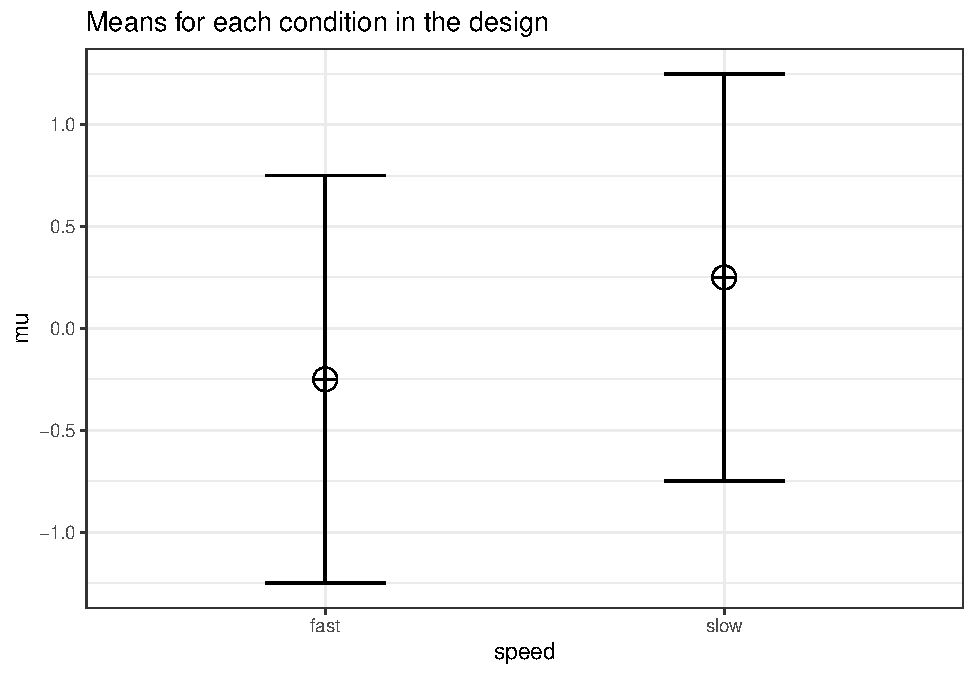
\includegraphics{SuperpowerValidation_files/figure-latex/unnamed-chunk-88-1.pdf}

\begin{Shaded}
\begin{Highlighting}[]
\NormalTok{alpha\_level }\OtherTok{\textless{}{-}} \FloatTok{0.05}
\end{Highlighting}
\end{Shaded}

\begin{Shaded}
\begin{Highlighting}[]
\NormalTok{simulation\_result }\OtherTok{\textless{}{-}} \FunctionTok{ANOVA\_power}\NormalTok{(design\_result, }
                                 \AttributeTok{alpha\_level =}\NormalTok{ alpha\_level, }
                                 \AttributeTok{nsims =}\NormalTok{ nsims, }\AttributeTok{verbose =} \ConstantTok{FALSE}\NormalTok{)}
\end{Highlighting}
\end{Shaded}

\newpage

\begin{table}[!h]

\caption{\label{tab:unnamed-chunk-90}Simulated ANOVA Result}
\centering
\begin{tabular}[t]{l|r|r}
\hline
  & power & effect\_size\\
\hline
anova\_speed & 81.02 & 0.2160964\\
\hline
\end{tabular}
\end{table}

\begin{table}[!h]

\caption{\label{tab:unnamed-chunk-92}Exact ANOVA Result}
\centering
\begin{tabular}[t]{l|r|r|r|r}
\hline
  & power & partial\_eta\_squared & cohen\_f & non\_centrality\\
\hline
speed & 80.77775 & 0.2048193 & 0.5075192 & 8.5\\
\hline
\end{tabular}
\end{table}

The results of the simulation are indeed very close to 80.777\%. Note that the simulation calculates Cohen's dz effect sizes for paired comparisons - which here given the correlation of 0.5 is also 0.5 for a medium effect size.

\newpage

We should see a larger dz if we increase the correlation, keeping the sample size the same, following the example in g*power above. We repeat the simulation, and the only difference is a correlation between dependent variables of 0.7. This should yield an effect size dz = 0.6454972.

\begin{Shaded}
\begin{Highlighting}[]
\NormalTok{K }\OtherTok{\textless{}{-}} \DecValTok{2}
\NormalTok{n }\OtherTok{\textless{}{-}} \DecValTok{21}
\NormalTok{sd }\OtherTok{\textless{}{-}} \DecValTok{1}
\NormalTok{r }\OtherTok{\textless{}{-}} \FloatTok{0.7}
\NormalTok{alpha }\OtherTok{=} \FloatTok{0.05}
\NormalTok{f }\OtherTok{\textless{}{-}} \FloatTok{0.25}
\NormalTok{f2 }\OtherTok{\textless{}{-}}\NormalTok{ f}\SpecialCharTok{\^{}}\DecValTok{2}
\NormalTok{ES }\OtherTok{\textless{}{-}}\NormalTok{ f2}\SpecialCharTok{/}\NormalTok{(f2 }\SpecialCharTok{+} \DecValTok{1}\NormalTok{)}
\NormalTok{ES}
\end{Highlighting}
\end{Shaded}

\begin{verbatim}
## [1] 0.05882353
\end{verbatim}

\begin{Shaded}
\begin{Highlighting}[]
\NormalTok{mu }\OtherTok{\textless{}{-}} \FunctionTok{mu\_from\_ES}\NormalTok{(}\AttributeTok{K =}\NormalTok{ K, }\AttributeTok{ES =}\NormalTok{ ES)}
\NormalTok{design }\OtherTok{=} \FunctionTok{paste}\NormalTok{(K,}\StringTok{"w"}\NormalTok{,}\AttributeTok{sep =} \StringTok{""}\NormalTok{)}
\NormalTok{labelnames }\OtherTok{\textless{}{-}} \FunctionTok{c}\NormalTok{(}\StringTok{"speed"}\NormalTok{, }\StringTok{"fast"}\NormalTok{, }\StringTok{"slow"}\NormalTok{)}
\NormalTok{design\_result }\OtherTok{\textless{}{-}} \FunctionTok{ANOVA\_design}\NormalTok{(}\AttributeTok{design =}\NormalTok{ design,}
                   \AttributeTok{n =}\NormalTok{ n, }\AttributeTok{mu =}\NormalTok{ mu, }\AttributeTok{sd =}\NormalTok{ sd, }\AttributeTok{r =}\NormalTok{ r, }
                   \AttributeTok{labelnames =}\NormalTok{ labelnames)}
\end{Highlighting}
\end{Shaded}

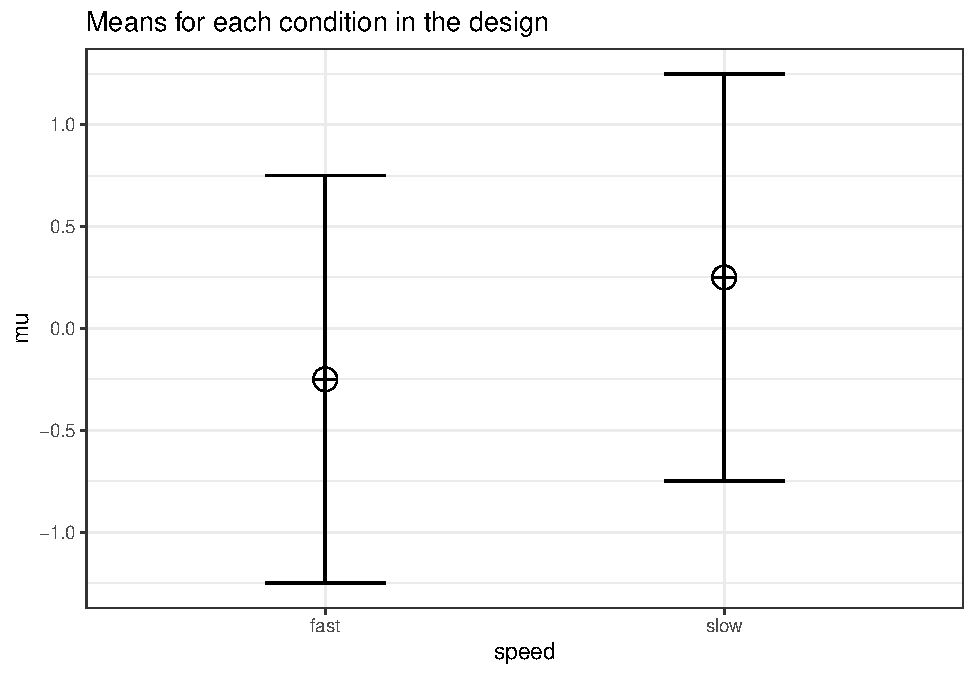
\includegraphics{SuperpowerValidation_files/figure-latex/unnamed-chunk-93-1.pdf}

\begin{Shaded}
\begin{Highlighting}[]
\NormalTok{alpha\_level }\OtherTok{\textless{}{-}} \FloatTok{0.05}
\end{Highlighting}
\end{Shaded}

\begin{table}[!h]

\caption{\label{tab:unnamed-chunk-94}Covariance-Variance Matrix}
\centering
\begin{tabular}[t]{l|r|r}
\hline
  & fast & slow\\
\hline
fast & 1.0 & 0.7\\
\hline
slow & 0.7 & 1.0\\
\hline
\end{tabular}
\end{table}
\newpage

\begin{Shaded}
\begin{Highlighting}[]
\NormalTok{simulation\_result }\OtherTok{\textless{}{-}} \FunctionTok{ANOVA\_power}\NormalTok{(design\_result, }
                                 \AttributeTok{alpha\_level =}\NormalTok{ alpha\_level, }
                                 \AttributeTok{nsims =}\NormalTok{ nsims,}
                                 \AttributeTok{verbose =} \ConstantTok{FALSE}\NormalTok{)}
\end{Highlighting}
\end{Shaded}

\begin{table}[!h]

\caption{\label{tab:unnamed-chunk-96}Simulated ANOVA Result}
\centering
\begin{tabular}[t]{l|r|r}
\hline
  & power & effect\_size\\
\hline
anova\_speed & 79.99 & 0.3158324\\
\hline
\end{tabular}
\end{table}

\begin{Shaded}
\begin{Highlighting}[]
\NormalTok{exact\_result }\OtherTok{\textless{}{-}} \FunctionTok{ANOVA\_exact}\NormalTok{(design\_result,}
                            \AttributeTok{alpha\_level =}\NormalTok{ alpha\_level,}
                            \AttributeTok{verbose =} \ConstantTok{FALSE}\NormalTok{)}
\end{Highlighting}
\end{Shaded}

\begin{table}[!h]

\caption{\label{tab:unnamed-chunk-98}Exact ANOVA Result}
\centering
\begin{tabular}[t]{l|r|r|r|r}
\hline
  & power & partial\_eta\_squared & cohen\_f & non\_centrality\\
\hline
speed & 80.33235 & 0.3043478 & 0.6614378 & 8.75\\
\hline
\end{tabular}
\end{table}

\begin{Shaded}
\begin{Highlighting}[]
\CommentTok{\#relation dz and f for within designs }
\NormalTok{f }\OtherTok{\textless{}{-}} \FloatTok{0.5}\SpecialCharTok{*}\FloatTok{0.6454972}
\NormalTok{f }
\end{Highlighting}
\end{Shaded}

\begin{verbatim}
## [1] 0.3227486
\end{verbatim}

Entering this f in g*power, with a correlation of 0.5, yields the same as entering \texttt{f\ =\ 0.25} and \texttt{correlation\ =\ 0.7}.

\newpage

\hypertarget{part-2}{%
\section{Part 2}\label{part-2}}

Here, we will examine a repeated measures experiment with 3 within-subject conditions, to illustrate how a repeated measures ANOVA extends a dependent \emph{t}-test with 3 groups.

In the example for a two-group within design we provided a specific formula for the sample size benefit for two groups. The sample size needed in within-designs (NW) with more than 2 conditions, relative to the sample needed in between-designs (NB), assuming normal distributions and compound symmetry, and ignoring the difference in degrees of freedom between the two types of tests, is (from \citet{maxwell_designing_2004}, p.~562, formula 47):

\(N_{W}=\frac{N_{B}(1-\rho)}{a}\)

Where ``a'' is the number of within-subject levels.

\hypertarget{the-relation-between-cohens-f-and-cohens-d}{%
\subsection{The relation between Cohen's f and Cohen's d}\label{the-relation-between-cohens-f-and-cohens-d}}

Whereas in the case of a repeated measures ANOVA with 2 groups we could explain the principles of a power analysis by comparing our test against a \emph{t}-test and Cohen's d, this becomes more difficult when we have more than 2 groups. It is more useful to explain how to directly calculate Cohen's \emph{f}, the effect size used in power analyses for ANOVA. Cohen's \emph{f} is calculated following \citet{cohen1988spa}, formula 8.2.1 and 8.2.2:

\(f = \sqrt{\frac{\frac{\sum(\mu-\overline{\mu})^2)}N}\sigma}\)

Imagine we have a within-subject experiment with 3 conditions. We ask people what they mood is when their alarm clock wakes them up, when they wake up naturally on a week day, and when they wake up naturally on a weekend day. Based on pilot data, we expect the means (on a 7 point validated mood scale) are 3.8, 4.2, and 4.3. The standard deviation is 0.9, and the correlation between the dependent measurements is 0.7. We can calculate Cohen's \emph{f} for the ANOVA, and Cohen's dz for the contrasts:

\begin{Shaded}
\begin{Highlighting}[]
\NormalTok{mu }\OtherTok{\textless{}{-}} \FunctionTok{c}\NormalTok{(}\FloatTok{3.8}\NormalTok{, }\FloatTok{4.2}\NormalTok{, }\FloatTok{4.3}\NormalTok{)}
\NormalTok{sd }\OtherTok{\textless{}{-}} \FloatTok{0.9}
\NormalTok{f }\OtherTok{\textless{}{-}} \FunctionTok{sqrt}\NormalTok{(}\FunctionTok{sum}\NormalTok{((mu }\SpecialCharTok{{-}} \FunctionTok{mean}\NormalTok{(mu)) }\SpecialCharTok{\^{}} \DecValTok{2}\NormalTok{) }\SpecialCharTok{/} \FunctionTok{length}\NormalTok{(mu)) }\SpecialCharTok{/}\NormalTok{ sd }
\CommentTok{\#Cohen, 1988, formula 8.2.1 and 8.2.2}
\NormalTok{  f}
\end{Highlighting}
\end{Shaded}

\begin{verbatim}
## [1] 0.2400274
\end{verbatim}

\begin{Shaded}
\begin{Highlighting}[]
\NormalTok{  r }\OtherTok{\textless{}{-}} \FloatTok{0.7}
\NormalTok{  (}\FloatTok{4.2} \SpecialCharTok{{-}} \FloatTok{3.8}\NormalTok{) }\SpecialCharTok{/} \FloatTok{0.9} \SpecialCharTok{/} \FunctionTok{sqrt}\NormalTok{(}\DecValTok{2} \SpecialCharTok{*}\NormalTok{ (}\DecValTok{1} \SpecialCharTok{{-}}\NormalTok{ r))}
\end{Highlighting}
\end{Shaded}

\begin{verbatim}
## [1] 0.5737753
\end{verbatim}

\begin{Shaded}
\begin{Highlighting}[]
\NormalTok{  (}\FloatTok{4.3} \SpecialCharTok{{-}} \FloatTok{3.8}\NormalTok{) }\SpecialCharTok{/} \FloatTok{0.9} \SpecialCharTok{/} \FunctionTok{sqrt}\NormalTok{(}\DecValTok{2} \SpecialCharTok{*}\NormalTok{ (}\DecValTok{1} \SpecialCharTok{{-}}\NormalTok{ r))}
\end{Highlighting}
\end{Shaded}

\begin{verbatim}
## [1] 0.7172191
\end{verbatim}

\begin{Shaded}
\begin{Highlighting}[]
\NormalTok{  (}\FloatTok{4.3} \SpecialCharTok{{-}} \FloatTok{4.2}\NormalTok{) }\SpecialCharTok{/} \FloatTok{0.9} \SpecialCharTok{/} \FunctionTok{sqrt}\NormalTok{(}\DecValTok{2} \SpecialCharTok{*}\NormalTok{ (}\DecValTok{1} \SpecialCharTok{{-}}\NormalTok{ r))}
\end{Highlighting}
\end{Shaded}

\begin{verbatim}
## [1] 0.1434438
\end{verbatim}

The relation between Cohen's d or dz and Cohen's \emph{f} becomes more difficult when there are multiple groups, because the relationship depends on the pattern of the means. \citet{cohen1988spa} presents calculations for three patterns, minimal variability (for example, for 5 means: -0.25, 0, 0, 0, 0.25), medium variability (for example, for 5 means: -0.25, -0.25, 0.25, 0.25, 0.25 or -0.25, -0.25, -0.25, 0.25, 0.25). For these three patterns, formula's are available that compute Cohen's \emph{f} from Cohen's d, where d is the effect size calculated for the difference between the largest and smallest mean (if the largest mean is 0.25 and the smallest mean is -0.25, 0.25 - -0.25 = 0.5, so d is 0.5 divided by the standard deviation of 0.9). In our example, d would be (4.3-3.8)/0.9 = 0.5555556. If we divide this value by \texttt{sqrt(2*(1-r))} we have dz = 0.5555556/0.7745967 = 0.7172191.

We have created a custom function that will calculate f from d, based on a specification of one of the three patterns of means. Our pattern is most similar (but not identical) to a maximum variability pattern (two means are high, one is lower). So we could attempt to calculate f from d (0.5555556), by calculating d from the largest and smallest mean.

This function allows you to calculate f, d and eta squared
following \citet{cohen1988spa}, p 277. The patterns are:
1. Minimum variability: one mean at each end of d, the remaining k- 2 means all at the midpoint.
2. Intermediate variability: the k means equally spaced over d.
3. Maximum variability: the means all at the end points of d.

For each of these patterns, there is a fixed relationship between f and d for any given number of means, k.

\textbf{Pattern 1}
For any given range of means, d, the minimum standard deviation, f1, results when the remaining k - 2 means are concentrated at the mean of the means (0 when expressed in standard units), i.e., half-way between the largest and smallest.

\textbf{Pattern 2}
A pattern of medium variability results when the k means are equally spaced over the range, and therefore at intervals of d/(k- 1).

\textbf{Pattern 3}
It is demonstrable and intuitively evident that for any given range the dispersion which yields the maximum standard deviation has the k means falling at both extremes of the range. When k is even, !k fall at - !d and the other !k fall at + !d; when k is odd, (k + 1 )/2 of the means fall at either end and the (k- 1)/2 remaining means at the other. With this pattern, for all even numbers of means, use formula (8.2.12). When k is odd, and there is thus one more mean at one extreme than at the other, use formula (8.2.13).

\begin{Shaded}
\begin{Highlighting}[]
\NormalTok{calc\_f\_d\_eta }\OtherTok{\textless{}{-}} \ControlFlowTok{function}\NormalTok{(mu, sd, variability)\{}
  \ControlFlowTok{if}\NormalTok{ (variability }\SpecialCharTok{==} \StringTok{"minimum"}\NormalTok{) \{}
\NormalTok{    k }\OtherTok{=} \FunctionTok{length}\NormalTok{(mu)}
\NormalTok{    d }\OtherTok{\textless{}{-}}\NormalTok{ (}\FunctionTok{max}\NormalTok{(mu) }\SpecialCharTok{{-}} \FunctionTok{min}\NormalTok{(mu)) }\SpecialCharTok{/}\NormalTok{ sd}
\NormalTok{    f }\OtherTok{\textless{}{-}}\NormalTok{ d }\SpecialCharTok{*} \FunctionTok{sqrt}\NormalTok{(}\DecValTok{1} \SpecialCharTok{/}\NormalTok{ (}\DecValTok{2} \SpecialCharTok{*}\NormalTok{ k))}
\NormalTok{    f2 }\OtherTok{\textless{}{-}}\NormalTok{ f }\SpecialCharTok{\^{}} \DecValTok{2}
\NormalTok{    ES }\OtherTok{\textless{}{-}}\NormalTok{ f2 }\SpecialCharTok{/}\NormalTok{ (f2 }\SpecialCharTok{+} \DecValTok{1}\NormalTok{)}
\NormalTok{  \}}
  \ControlFlowTok{if}\NormalTok{ (variability }\SpecialCharTok{==} \StringTok{"medium"}\NormalTok{) \{}
\NormalTok{    k }\OtherTok{=} \FunctionTok{length}\NormalTok{(mu)}
\NormalTok{    d }\OtherTok{\textless{}{-}}\NormalTok{ (}\FunctionTok{max}\NormalTok{(mu) }\SpecialCharTok{{-}} \FunctionTok{min}\NormalTok{(mu)) }\SpecialCharTok{/}\NormalTok{ sd}
\NormalTok{    f }\OtherTok{\textless{}{-}}\NormalTok{ (d }\SpecialCharTok{/} \DecValTok{2}\NormalTok{) }\SpecialCharTok{*} \FunctionTok{sqrt}\NormalTok{((k }\SpecialCharTok{+} \DecValTok{1}\NormalTok{) }\SpecialCharTok{/}\NormalTok{ (}\DecValTok{3} \SpecialCharTok{*}\NormalTok{ (k }\SpecialCharTok{{-}} \DecValTok{1}\NormalTok{)))}
\NormalTok{    f2 }\OtherTok{\textless{}{-}}\NormalTok{ f }\SpecialCharTok{\^{}} \DecValTok{2}
\NormalTok{    ES }\OtherTok{\textless{}{-}}\NormalTok{ f2 }\SpecialCharTok{/}\NormalTok{ (f2 }\SpecialCharTok{+} \DecValTok{1}\NormalTok{)}
\NormalTok{  \}}
  \ControlFlowTok{if}\NormalTok{ (variability }\SpecialCharTok{==} \StringTok{"maximum"}\NormalTok{) \{}
\NormalTok{    k }\OtherTok{=} \FunctionTok{length}\NormalTok{(mu)}
\NormalTok{    d }\OtherTok{\textless{}{-}}\NormalTok{ (}\FunctionTok{max}\NormalTok{(mu) }\SpecialCharTok{{-}} \FunctionTok{min}\NormalTok{(mu)) }\SpecialCharTok{/}\NormalTok{ sd}
\NormalTok{    f }\OtherTok{\textless{}{-}} \FunctionTok{ifelse}\NormalTok{(k }\SpecialCharTok{\%\%} \DecValTok{2} \SpecialCharTok{==} \DecValTok{0}\NormalTok{, .}\DecValTok{5} \SpecialCharTok{*}\NormalTok{ d, d }\SpecialCharTok{*}\NormalTok{ (}\FunctionTok{sqrt}\NormalTok{(k }\SpecialCharTok{\^{}} \DecValTok{2} \SpecialCharTok{{-}} \DecValTok{1}\NormalTok{) }\SpecialCharTok{/}\NormalTok{ (}\DecValTok{2} \SpecialCharTok{*}\NormalTok{ k)))}
\NormalTok{    f2 }\OtherTok{\textless{}{-}}\NormalTok{ f }\SpecialCharTok{\^{}} \DecValTok{2}
\NormalTok{    ES }\OtherTok{\textless{}{-}}\NormalTok{ f2 }\SpecialCharTok{/}\NormalTok{ (f2 }\SpecialCharTok{+} \DecValTok{1}\NormalTok{)}
\NormalTok{  \}}
  \FunctionTok{invisible}\NormalTok{(}\FunctionTok{list}\NormalTok{(}\AttributeTok{mu =}\NormalTok{ mu,}
                 \AttributeTok{sd =}\NormalTok{ sd,}
                 \AttributeTok{d =}\NormalTok{ d,}
                 \AttributeTok{f =}\NormalTok{ f,}
                 \AttributeTok{f2 =}\NormalTok{ f2,}
                 \AttributeTok{ES =}\NormalTok{ ES))}
\NormalTok{\}}
\NormalTok{res }\OtherTok{\textless{}{-}} \FunctionTok{calc\_f\_d\_eta}\NormalTok{(}\AttributeTok{mu =}\NormalTok{ mu, }\AttributeTok{sd =}\NormalTok{ sd, }\AttributeTok{variability =} \StringTok{"maximum"}\NormalTok{)}
\NormalTok{res}\SpecialCharTok{$}\NormalTok{f}
\end{Highlighting}
\end{Shaded}

\begin{verbatim}
## [1] 0.2618914
\end{verbatim}

\begin{Shaded}
\begin{Highlighting}[]
\NormalTok{res}\SpecialCharTok{$}\NormalTok{d}
\end{Highlighting}
\end{Shaded}

\begin{verbatim}
## [1] 0.5555556
\end{verbatim}

We see the Cohen's \emph{f} value is 0.2618914 and d = 0.5555556. The Cohen's \emph{f} is not perfectly accurate - it is assuming the pattern of means is 3.8, 4.3, 4.3, and not 3.8, 4.2, 4.3. If the means and sds are known, it is best to calculate Cohen's \emph{f} directly from these values.

\hypertarget{three-within-conditions-medium-effect-size}{%
\subsection{Three within conditions, medium effect size}\label{three-within-conditions-medium-effect-size}}

We can perform power analyses for within designs using simulations. We set groups to 3 for the simulation, n = 20, and the correlation between dependent variables to 0.8. If the true effect size is f = 0.25, and the alpha level is 0.05, the power is 96.6\%. In this case, we simulate data with means -0.3061862, 0.0000000, and 0.3061862, and set the sd to 1.

\begin{Shaded}
\begin{Highlighting}[]
\NormalTok{K }\OtherTok{\textless{}{-}} \DecValTok{3}
\NormalTok{n }\OtherTok{\textless{}{-}} \DecValTok{20}
\NormalTok{sd }\OtherTok{\textless{}{-}} \DecValTok{1}
\NormalTok{r }\OtherTok{\textless{}{-}} \FloatTok{0.8}
\NormalTok{alpha }\OtherTok{=} \FloatTok{0.05}
\NormalTok{f }\OtherTok{\textless{}{-}} \FloatTok{0.25}
\NormalTok{f2 }\OtherTok{\textless{}{-}}\NormalTok{ f}\SpecialCharTok{\^{}}\DecValTok{2}
\NormalTok{ES }\OtherTok{\textless{}{-}}\NormalTok{ f2 }\SpecialCharTok{/}\NormalTok{ (f2 }\SpecialCharTok{+} \DecValTok{1}\NormalTok{)}
\NormalTok{ES}
\end{Highlighting}
\end{Shaded}

\begin{verbatim}
## [1] 0.05882353
\end{verbatim}

\begin{Shaded}
\begin{Highlighting}[]
\NormalTok{mu }\OtherTok{\textless{}{-}} \FunctionTok{mu\_from\_ES}\NormalTok{(}\AttributeTok{K =}\NormalTok{ K, }\AttributeTok{ES =}\NormalTok{ ES)}

\CommentTok{\#Cohen, 1988, formula 8.2.1 and 8.2.2}
\FunctionTok{sqrt}\NormalTok{(}\FunctionTok{sum}\NormalTok{((mu }\SpecialCharTok{{-}} \FunctionTok{mean}\NormalTok{(mu)) }\SpecialCharTok{\^{}} \DecValTok{2}\NormalTok{) }\SpecialCharTok{/} \FunctionTok{length}\NormalTok{(mu)) }\SpecialCharTok{/}\NormalTok{ sd }
\end{Highlighting}
\end{Shaded}

\begin{verbatim}
## [1] 0.25
\end{verbatim}

\begin{Shaded}
\begin{Highlighting}[]
\NormalTok{design }\OtherTok{=} \FunctionTok{paste}\NormalTok{(K, }\StringTok{"w"}\NormalTok{, }\AttributeTok{sep =} \StringTok{""}\NormalTok{)}
\NormalTok{labelnames }\OtherTok{\textless{}{-}} \FunctionTok{c}\NormalTok{(}\StringTok{"speed"}\NormalTok{, }\StringTok{"fast"}\NormalTok{, }\StringTok{"medium"}\NormalTok{, }\StringTok{"slow"}\NormalTok{)}
\NormalTok{design\_result }\OtherTok{\textless{}{-}} \FunctionTok{ANOVA\_design}\NormalTok{(}\AttributeTok{design =}\NormalTok{ design,}
                   \AttributeTok{n =}\NormalTok{ n, }
                   \AttributeTok{mu =}\NormalTok{ mu, }
                   \AttributeTok{sd =}\NormalTok{ sd, }
                   \AttributeTok{r =}\NormalTok{ r, }
                   \AttributeTok{labelnames =}\NormalTok{ labelnames)}
\end{Highlighting}
\end{Shaded}

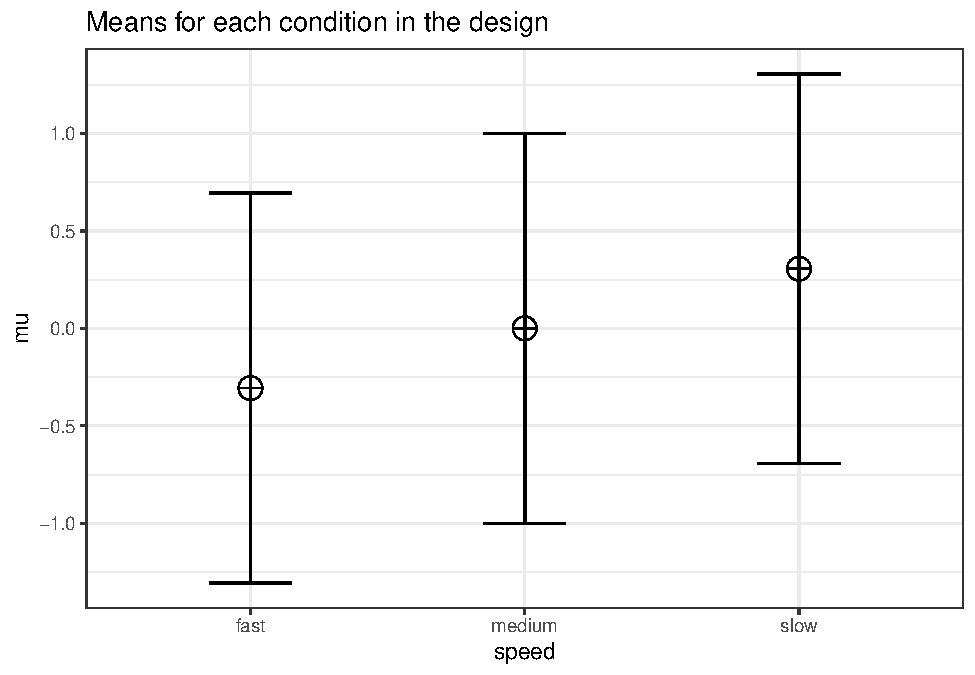
\includegraphics{SuperpowerValidation_files/figure-latex/unnamed-chunk-102-1.pdf}

\begin{Shaded}
\begin{Highlighting}[]
\NormalTok{alpha\_level }\OtherTok{\textless{}{-}} \FloatTok{0.05}
\end{Highlighting}
\end{Shaded}

\begin{Shaded}
\begin{Highlighting}[]
\NormalTok{simulation\_result }\OtherTok{\textless{}{-}} \FunctionTok{ANOVA\_power}\NormalTok{(design\_result, }
                                 \AttributeTok{alpha\_level =}\NormalTok{ alpha\_level, }
                                 \AttributeTok{nsims =}\NormalTok{ nsims,}
                                 \AttributeTok{verbose =} \ConstantTok{FALSE}\NormalTok{)}
\end{Highlighting}
\end{Shaded}

\begin{table}[!h]

\caption{\label{tab:unnamed-chunk-104}Simulated ANOVA Result}
\centering
\begin{tabular}[t]{l|r|r}
\hline
  & power & effect\_size\\
\hline
anova\_speed & 96.89 & 0.347031\\
\hline
\end{tabular}
\end{table}

\begin{Shaded}
\begin{Highlighting}[]
\NormalTok{exact\_result }\OtherTok{\textless{}{-}} \FunctionTok{ANOVA\_exact}\NormalTok{(design\_result,}
                            \AttributeTok{alpha\_level =}\NormalTok{ alpha\_level,}
                            \AttributeTok{verbose =} \ConstantTok{FALSE}\NormalTok{)}
\end{Highlighting}
\end{Shaded}

\begin{table}[!h]

\caption{\label{tab:unnamed-chunk-106}Exact ANOVA Result}
\centering
\begin{tabular}[t]{l|r|r|r|r}
\hline
  & power & partial\_eta\_squared & cohen\_f & non\_centrality\\
\hline
speed & 96.91634 & 0.3303965 & 0.7024394 & 18.75\\
\hline
\end{tabular}
\end{table}

The results of the simulation are indeed very close to 96.9\%.
\newpage

We can see this is in line with the power estimate from Gpower:

\includegraphics{screenshots/gpower_12.png}

\newpage

We can also validate this by creating the code to do a power analysis in R from scratch:

\begin{Shaded}
\begin{Highlighting}[]
\NormalTok{K }\OtherTok{\textless{}{-}} \DecValTok{3} \CommentTok{\#three groups}
\NormalTok{n }\OtherTok{\textless{}{-}} \DecValTok{20}
\NormalTok{sd }\OtherTok{\textless{}{-}} \DecValTok{1}
\NormalTok{r }\OtherTok{\textless{}{-}} \FloatTok{0.8}
\NormalTok{alpha }\OtherTok{=} \FloatTok{0.05}
\NormalTok{f }\OtherTok{\textless{}{-}} \FloatTok{0.25}
\NormalTok{f2 }\OtherTok{\textless{}{-}}\NormalTok{ f}\SpecialCharTok{\^{}}\DecValTok{2}
\NormalTok{ES }\OtherTok{\textless{}{-}}\NormalTok{ f2 }\SpecialCharTok{/}\NormalTok{ (f2 }\SpecialCharTok{+} \DecValTok{1}\NormalTok{)}
\NormalTok{ES}
\end{Highlighting}
\end{Shaded}

\begin{verbatim}
## [1] 0.05882353
\end{verbatim}

\begin{Shaded}
\begin{Highlighting}[]
\NormalTok{mu }\OtherTok{\textless{}{-}} \FunctionTok{mu\_from\_ES}\NormalTok{(}\AttributeTok{K =}\NormalTok{ K, }\AttributeTok{ES =}\NormalTok{ ES)}
\NormalTok{design }\OtherTok{=} \FunctionTok{paste}\NormalTok{(K, }\StringTok{"w"}\NormalTok{, }\AttributeTok{sep =} \StringTok{""}\NormalTok{)}
\NormalTok{labelnames }\OtherTok{\textless{}{-}} \FunctionTok{c}\NormalTok{(}\StringTok{"speed"}\NormalTok{, }\StringTok{"fast"}\NormalTok{, }\StringTok{"medium"}\NormalTok{, }\StringTok{"slow"}\NormalTok{)}
\NormalTok{design\_result }\OtherTok{\textless{}{-}} \FunctionTok{ANOVA\_design}\NormalTok{(}\AttributeTok{design =}\NormalTok{ design,}
                   \AttributeTok{n =}\NormalTok{ n, }
                   \AttributeTok{mu =}\NormalTok{ mu, }
                   \AttributeTok{sd =}\NormalTok{ sd, }
                   \AttributeTok{r =}\NormalTok{ r, }
                   \AttributeTok{labelnames =}\NormalTok{ labelnames)}
\end{Highlighting}
\end{Shaded}

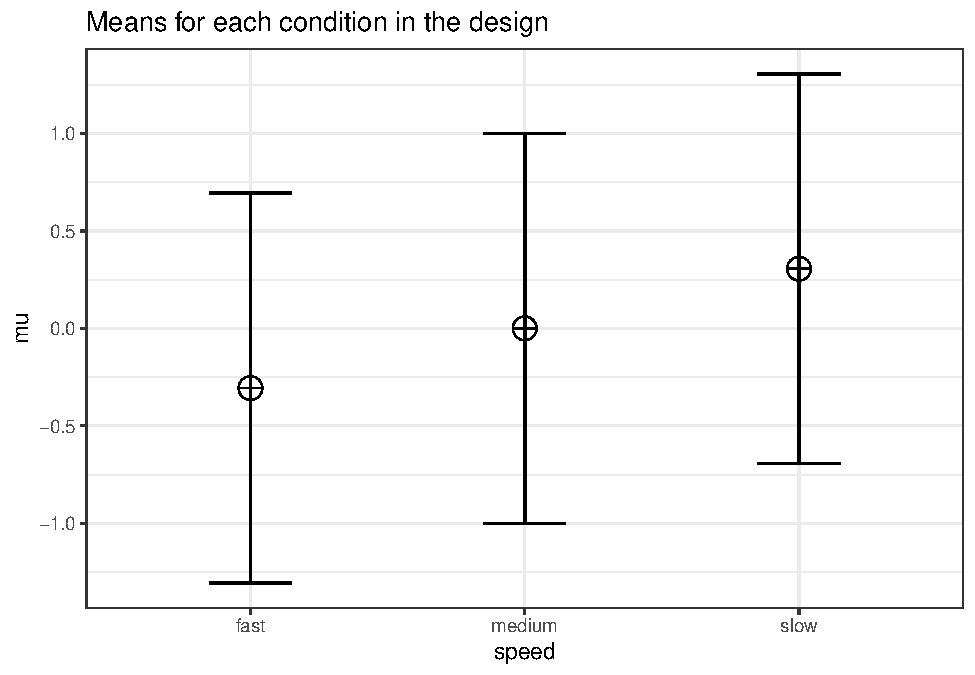
\includegraphics{SuperpowerValidation_files/figure-latex/unnamed-chunk-107-1.pdf}

\begin{Shaded}
\begin{Highlighting}[]
\FunctionTok{power\_oneway\_within}\NormalTok{(design\_result)}\SpecialCharTok{$}\NormalTok{power}
\end{Highlighting}
\end{Shaded}

\begin{verbatim}
## [1] 96.91634
\end{verbatim}

\begin{Shaded}
\begin{Highlighting}[]
\FunctionTok{power\_oneway\_within}\NormalTok{(design\_result)}\SpecialCharTok{$}\NormalTok{eta\_p\_2}
\end{Highlighting}
\end{Shaded}

\begin{verbatim}
## [1] 0.05882353
\end{verbatim}

\begin{Shaded}
\begin{Highlighting}[]
\FunctionTok{power\_oneway\_within}\NormalTok{(design\_result)}\SpecialCharTok{$}\NormalTok{eta\_p\_2\_SPSS}
\end{Highlighting}
\end{Shaded}

\begin{verbatim}
## [1] 0.3303965
\end{verbatim}

\begin{Shaded}
\begin{Highlighting}[]
\FunctionTok{power\_oneway\_within}\NormalTok{(design\_result)}\SpecialCharTok{$}\NormalTok{Cohen\_f}
\end{Highlighting}
\end{Shaded}

\begin{verbatim}
## [1] 0.25
\end{verbatim}

\begin{Shaded}
\begin{Highlighting}[]
\FunctionTok{power\_oneway\_within}\NormalTok{(design\_result)}\SpecialCharTok{$}\NormalTok{Cohen\_f\_SPSS}
\end{Highlighting}
\end{Shaded}

\begin{verbatim}
## [1] 0.7024394
\end{verbatim}

\newpage

We can even check the calculation of Cohen's \emph{f} SPSS style in g*power We take the g*power settings as illustrated above. We click the `Options' button, and check the radio button next to `As in SPSS'. Click ok, and you will notice that the `Corr among rep measures' field has disappeared. The correlation does not need to be entered seperately, but is incorporated in Cohen's \emph{f}. The value of Cohen's \emph{f}, which was 0.25, has changed into 0.7024394. This is the SPSS equivalent. The value is much larger. This value, and it's corresponding partial eta-squared, incorporate the correlation between observations.

\includegraphics{screenshots/gpower_14.png}

\newpage

\hypertarget{part-3}{%
\section{Part 3}\label{part-3}}

We first repeat the simulation by Brysbaert:

\begin{Shaded}
\begin{Highlighting}[]
\CommentTok{\# give sample size}
\NormalTok{N }\OtherTok{=} \DecValTok{75}
\CommentTok{\# give effect size d}
\NormalTok{d1 }\OtherTok{=}\NormalTok{ .}\DecValTok{4} \CommentTok{\#difference between the extremes}
\NormalTok{d2 }\OtherTok{=}\NormalTok{ .}\DecValTok{4} \CommentTok{\#third condition goes with the highest extreme}
\CommentTok{\# give the correlation between the conditions}
\NormalTok{r }\OtherTok{=}\NormalTok{ .}\DecValTok{5}
\CommentTok{\# give number of simulations}
\NormalTok{nSim }\OtherTok{=}\NormalTok{ nsims}
\CommentTok{\# give alpha levels}
\NormalTok{alpha1 }\OtherTok{=}\NormalTok{ .}\DecValTok{05} \CommentTok{\#alpha level for the omnibus ANOVA}
\NormalTok{alpha2 }\OtherTok{=}\NormalTok{ .}\DecValTok{05} \CommentTok{\#also adjusted from original by DL}
\end{Highlighting}
\end{Shaded}

\begin{Shaded}
\begin{Highlighting}[]
\CommentTok{\# create vectors to store p{-}values}
\NormalTok{p1 }\OtherTok{\textless{}{-}} \FunctionTok{numeric}\NormalTok{(nSim) }\CommentTok{\#p{-}value omnibus ANOVA}
\NormalTok{p2 }\OtherTok{\textless{}{-}} \FunctionTok{numeric}\NormalTok{(nSim) }\CommentTok{\#p{-}value first post hoc test}
\NormalTok{p3 }\OtherTok{\textless{}{-}} \FunctionTok{numeric}\NormalTok{(nSim) }\CommentTok{\#p{-}value second post hoc test}
\NormalTok{p4 }\OtherTok{\textless{}{-}} \FunctionTok{numeric}\NormalTok{(nSim) }\CommentTok{\#p{-}value third post hoc test}

\CommentTok{\# define correlation matrix}
\NormalTok{rho }\OtherTok{\textless{}{-}} \FunctionTok{cbind}\NormalTok{(}\FunctionTok{c}\NormalTok{(}\DecValTok{1}\NormalTok{, r, r), }\FunctionTok{c}\NormalTok{(r, }\DecValTok{1}\NormalTok{, r), }\FunctionTok{c}\NormalTok{(r, r, }\DecValTok{1}\NormalTok{))}
\CommentTok{\# define participant codes}
\NormalTok{part }\OtherTok{\textless{}{-}} \FunctionTok{paste}\NormalTok{(}\StringTok{"part"}\NormalTok{,}\FunctionTok{seq}\NormalTok{(}\DecValTok{1}\SpecialCharTok{:}\NormalTok{N))}
\ControlFlowTok{for}\NormalTok{ (i }\ControlFlowTok{in} \DecValTok{1}\SpecialCharTok{:}\NormalTok{nSim) \{}
  \CommentTok{\#for each simulated experiment}

\NormalTok{  data }\OtherTok{=} \FunctionTok{mvrnorm}\NormalTok{(}\AttributeTok{n =}\NormalTok{ N,}
  \AttributeTok{mu =} \FunctionTok{c}\NormalTok{(}\DecValTok{0}\NormalTok{, }\DecValTok{0}\NormalTok{, }\DecValTok{0}\NormalTok{),}
  \AttributeTok{Sigma =}\NormalTok{ rho)}
\NormalTok{  data[, }\DecValTok{2}\NormalTok{] }\OtherTok{=}\NormalTok{ data[, }\DecValTok{2}\NormalTok{] }\SpecialCharTok{+}\NormalTok{ d1}
\NormalTok{  data[, }\DecValTok{3}\NormalTok{] }\OtherTok{=}\NormalTok{ data[, }\DecValTok{3}\NormalTok{] }\SpecialCharTok{+}\NormalTok{ d2}
\NormalTok{  datalong }\OtherTok{=} \FunctionTok{c}\NormalTok{(data[, }\DecValTok{1}\NormalTok{], data[, }\DecValTok{2}\NormalTok{], data[, }\DecValTok{3}\NormalTok{])}
\NormalTok{  conds }\OtherTok{=} \FunctionTok{factor}\NormalTok{(}\FunctionTok{rep}\NormalTok{(letters[}\DecValTok{24}\SpecialCharTok{:}\DecValTok{26}\NormalTok{], }\AttributeTok{each =}\NormalTok{ N))}
\NormalTok{  partID }\OtherTok{=} \FunctionTok{factor}\NormalTok{(}\FunctionTok{rep}\NormalTok{(part, }\AttributeTok{times =} \DecValTok{3}\NormalTok{))}
\NormalTok{  output }\OtherTok{\textless{}{-}} \FunctionTok{data.frame}\NormalTok{(partID, conds, datalong)}
\NormalTok{  test }\OtherTok{\textless{}{-}} \FunctionTok{aov}\NormalTok{(datalong }\SpecialCharTok{\textasciitilde{}}\NormalTok{ conds }\SpecialCharTok{+} \FunctionTok{Error}\NormalTok{(partID }\SpecialCharTok{/}\NormalTok{ conds), }\AttributeTok{data =}\NormalTok{ output)}
\NormalTok{  tests }\OtherTok{\textless{}{-}}\NormalTok{ (}\FunctionTok{summary}\NormalTok{(test))}
\NormalTok{  p1[i] }\OtherTok{\textless{}{-}}\NormalTok{ tests}\SpecialCharTok{$}\StringTok{\textquotesingle{}Error: partID:conds\textquotesingle{}}\NormalTok{[[}\DecValTok{1}\NormalTok{]]}\SpecialCharTok{$}\StringTok{\textquotesingle{}Pr(\textgreater{}F)\textquotesingle{}}\NormalTok{[[}\DecValTok{1}\NormalTok{]]}
\NormalTok{  p2[i] }\OtherTok{\textless{}{-}} \FunctionTok{t.test}\NormalTok{(data[, }\DecValTok{1}\NormalTok{], data[, }\DecValTok{2}\NormalTok{], }\AttributeTok{paired =} \ConstantTok{TRUE}\NormalTok{)}\SpecialCharTok{$}\NormalTok{p.value}
\NormalTok{  p3[i] }\OtherTok{\textless{}{-}} \FunctionTok{t.test}\NormalTok{(data[, }\DecValTok{1}\NormalTok{], data[, }\DecValTok{3}\NormalTok{], }\AttributeTok{paired =} \ConstantTok{TRUE}\NormalTok{)}\SpecialCharTok{$}\NormalTok{p.value}
\NormalTok{  p4[i] }\OtherTok{\textless{}{-}} \FunctionTok{t.test}\NormalTok{(data[, }\DecValTok{2}\NormalTok{], data[, }\DecValTok{3}\NormalTok{], }\AttributeTok{paired =} \ConstantTok{TRUE}\NormalTok{)}\SpecialCharTok{$}\NormalTok{p.value}
\NormalTok{\}}
\end{Highlighting}
\end{Shaded}

\begin{Shaded}
\begin{Highlighting}[]
\CommentTok{\#printing all unique tests (adjusted code by DL)}
\FunctionTok{sum}\NormalTok{(p1 }\SpecialCharTok{\textless{}}\NormalTok{ alpha1) }\SpecialCharTok{/}\NormalTok{ nSim}
\FunctionTok{sum}\NormalTok{(p2 }\SpecialCharTok{\textless{}}\NormalTok{ alpha2) }\SpecialCharTok{/}\NormalTok{ nSim}
\FunctionTok{sum}\NormalTok{(p3 }\SpecialCharTok{\textless{}}\NormalTok{ alpha2) }\SpecialCharTok{/}\NormalTok{ nSim}
\FunctionTok{sum}\NormalTok{(p4 }\SpecialCharTok{\textless{}}\NormalTok{ alpha2) }\SpecialCharTok{/}\NormalTok{ nSim}
\end{Highlighting}
\end{Shaded}

\begin{verbatim}
## [1] 0.792
\end{verbatim}

\begin{verbatim}
## [1] 0.7576
\end{verbatim}

\begin{verbatim}
## [1] 0.7599
\end{verbatim}

\begin{verbatim}
## [1] 0.048
\end{verbatim}

\newpage

\hypertarget{part-4}{%
\section{Part 4}\label{part-4}}

\hypertarget{x2-anova-within-within-design}{%
\subsection{2x2 ANOVA, within-within design}\label{x2-anova-within-within-design}}

We can simulate a 2x2 ANOVA, both factors manipulated within participants, with a specific sample size and effect size, to achieve a desired statistical power.

As \citet{potvin2000statistical} explain, analytic procedures for a two-factor repeated measures ANOVA do not seem to exist. The main problem is quantifying the error variance (the denominator when calculating lambda or Cohen's \emph{f}). Simulation based aproaches provide a solution.

We can reproduce the simulation coded by \href{https://cognitivedatascientist.com/2015/12/14/power-simulation-in-r-the-repeated-measures-anova-5/}{Ben Amsel}

\begin{Shaded}
\begin{Highlighting}[]
\CommentTok{\# define the parameters}
\CommentTok{\# true effects (in this case, a double dissociation)}
\NormalTok{mu }\OtherTok{=} \FunctionTok{c}\NormalTok{(}\DecValTok{700}\NormalTok{, }\DecValTok{670}\NormalTok{, }\DecValTok{670}\NormalTok{, }\DecValTok{700}\NormalTok{) }
\NormalTok{sigma }\OtherTok{=} \DecValTok{150}  \CommentTok{\# population standard deviation}
\NormalTok{rho }\OtherTok{=} \FloatTok{0.75} \CommentTok{\# correlation between repeated measures}
\NormalTok{nsubs }\OtherTok{=} \DecValTok{25} \CommentTok{\# how many subjects?}
\NormalTok{nsims }\OtherTok{=}\NormalTok{ nsims }\CommentTok{\# how many simulation replicates?}
 
\CommentTok{\# create 2 factors representing the 2 independent variables}
\NormalTok{cond }\OtherTok{=} \FunctionTok{data.frame}\NormalTok{(}\AttributeTok{X1 =} \FunctionTok{rep}\NormalTok{(}\FunctionTok{factor}\NormalTok{(letters[}\DecValTok{1}\SpecialCharTok{:}\DecValTok{2}\NormalTok{]), nsubs }\SpecialCharTok{*} \DecValTok{2}\NormalTok{),}
                  \AttributeTok{X2 =} \FunctionTok{rep}\NormalTok{(}\FunctionTok{factor}\NormalTok{(letters[}\DecValTok{1}\SpecialCharTok{:}\DecValTok{2}\NormalTok{]), nsubs, }\AttributeTok{each =} \DecValTok{2}\NormalTok{))}
 
\CommentTok{\# create a subjects factor}
\NormalTok{subject }\OtherTok{=} \FunctionTok{factor}\NormalTok{(}\FunctionTok{sort}\NormalTok{(}\FunctionTok{rep}\NormalTok{(}\DecValTok{1}\SpecialCharTok{:}\NormalTok{nsubs, }\DecValTok{4}\NormalTok{)))}
 
\CommentTok{\# combine above into the design matrix}
\NormalTok{dm }\OtherTok{=} \FunctionTok{data.frame}\NormalTok{(subject, cond)}
\end{Highlighting}
\end{Shaded}

Build Sigma: the population variance-covariance matrix

\begin{Shaded}
\begin{Highlighting}[]
\CommentTok{\# create k x k matrix populated with sigma}
\NormalTok{sigma.mat }\OtherTok{\textless{}{-}} \FunctionTok{rep}\NormalTok{(sigma, }\DecValTok{4}\NormalTok{)}
\NormalTok{S }\OtherTok{\textless{}{-}}
  \FunctionTok{matrix}\NormalTok{(sigma.mat,}
  \AttributeTok{ncol =} \FunctionTok{length}\NormalTok{(sigma.mat),}
  \AttributeTok{nrow =} \FunctionTok{length}\NormalTok{(sigma.mat))}
 
\CommentTok{\# compute covariance between measures}
\NormalTok{Sigma }\OtherTok{\textless{}{-}} \FunctionTok{t}\NormalTok{(S) }\SpecialCharTok{*}\NormalTok{ S }\SpecialCharTok{*}\NormalTok{ rho  }
 
\CommentTok{\# put the variances on the diagonal }
\FunctionTok{diag}\NormalTok{(Sigma) }\OtherTok{\textless{}{-}}\NormalTok{ sigma}\SpecialCharTok{\^{}}\DecValTok{2}  
\end{Highlighting}
\end{Shaded}

Run the simulation

\begin{Shaded}
\begin{Highlighting}[]
\CommentTok{\# stack \textquotesingle{}nsims\textquotesingle{} individual data frames into one large data frame}
\NormalTok{df }\OtherTok{=}\NormalTok{ dm[}\FunctionTok{rep}\NormalTok{(}\FunctionTok{seq\_len}\NormalTok{(}\FunctionTok{nrow}\NormalTok{(dm)), nsims), ]}
 
\CommentTok{\# add an index column to track the simulation run}
\NormalTok{df}\SpecialCharTok{$}\NormalTok{simID }\OtherTok{=} \FunctionTok{sort}\NormalTok{(}\FunctionTok{rep}\NormalTok{(}\FunctionTok{seq\_len}\NormalTok{(nsims), }\FunctionTok{nrow}\NormalTok{(dm)))}
 
\CommentTok{\# sample the observed data from a multivariate normal distribution}
\CommentTok{\# using MASS::mvrnorm with the mu and Sigma created earlier}
\CommentTok{\# and bind to the existing df}
 

\NormalTok{make.y }\OtherTok{=} \FunctionTok{expression}\NormalTok{(}\FunctionTok{as.vector}\NormalTok{(}\FunctionTok{t}\NormalTok{(}\FunctionTok{mvrnorm}\NormalTok{(nsubs, mu, Sigma))))}
\NormalTok{df}\SpecialCharTok{$}\NormalTok{y }\OtherTok{=} \FunctionTok{as.vector}\NormalTok{(}\FunctionTok{replicate}\NormalTok{(nsims, }\FunctionTok{eval}\NormalTok{(make.y)))             }
 
\CommentTok{\# use do(), the general purpose complement to the specialized data }
\CommentTok{\# manipulation functions available in dplyr, to run the ANOVA on}
\CommentTok{\# each section of the grouped data frame created by group\_by}
 

\NormalTok{mods }\OtherTok{\textless{}{-}}\NormalTok{ df }\SpecialCharTok{\%\textgreater{}\%}
  \FunctionTok{group\_by}\NormalTok{(simID) }\SpecialCharTok{\%\textgreater{}\%}
  \FunctionTok{do}\NormalTok{(}\AttributeTok{model =} \FunctionTok{aov}\NormalTok{(y }\SpecialCharTok{\textasciitilde{}}\NormalTok{ X1 }\SpecialCharTok{*}\NormalTok{ X2 }\SpecialCharTok{+} \FunctionTok{Error}\NormalTok{(subject }\SpecialCharTok{/}\NormalTok{ (X1 }\SpecialCharTok{*}\NormalTok{ X2)), }
                 \AttributeTok{qr =} \ConstantTok{FALSE}\NormalTok{, }\AttributeTok{data =}\NormalTok{ .)) }
 
\CommentTok{\# extract p{-}values for each effect and store in a data frame}
\NormalTok{p\_val\_1 }\OtherTok{=} \FunctionTok{data.frame}\NormalTok{(}
\NormalTok{  mods }\SpecialCharTok{\%\textgreater{}\%} \FunctionTok{do}\NormalTok{(}\FunctionTok{as.data.frame}\NormalTok{(}\FunctionTok{tidy}\NormalTok{(.}\SpecialCharTok{$}\NormalTok{model[[}\DecValTok{3}\NormalTok{]])}\SpecialCharTok{$}\NormalTok{p.value[}\DecValTok{1}\NormalTok{])),}
\NormalTok{  mods }\SpecialCharTok{\%\textgreater{}\%} \FunctionTok{do}\NormalTok{(}\FunctionTok{as.data.frame}\NormalTok{(}\FunctionTok{tidy}\NormalTok{(.}\SpecialCharTok{$}\NormalTok{model[[}\DecValTok{4}\NormalTok{]])}\SpecialCharTok{$}\NormalTok{p.value[}\DecValTok{1}\NormalTok{])),}
\NormalTok{  mods }\SpecialCharTok{\%\textgreater{}\%} \FunctionTok{do}\NormalTok{(}\FunctionTok{as.data.frame}\NormalTok{(}\FunctionTok{tidy}\NormalTok{(.}\SpecialCharTok{$}\NormalTok{model[[}\DecValTok{5}\NormalTok{]])}\SpecialCharTok{$}\NormalTok{p.value[}\DecValTok{1}\NormalTok{])))}
\FunctionTok{colnames}\NormalTok{(p\_val\_1) }\OtherTok{=} \FunctionTok{c}\NormalTok{(}\StringTok{\textquotesingle{}X1\textquotesingle{}}\NormalTok{,}\StringTok{\textquotesingle{}X2\textquotesingle{}}\NormalTok{,}\StringTok{\textquotesingle{}Interaction\textquotesingle{}}\NormalTok{)}
\end{Highlighting}
\end{Shaded}

The empirical power is easy to compute, it's just the proportion of simulation runs where \emph{p} \textless{} .05.

\begin{Shaded}
\begin{Highlighting}[]
\NormalTok{power.res }\OtherTok{=} \FunctionTok{apply}\NormalTok{(}\FunctionTok{as.matrix}\NormalTok{(p\_val\_1), }\DecValTok{2}\NormalTok{, }
  \ControlFlowTok{function}\NormalTok{(x) }\FunctionTok{round}\NormalTok{(}\FunctionTok{mean}\NormalTok{(}\FunctionTok{ifelse}\NormalTok{(x }\SpecialCharTok{\textless{}}\NormalTok{ .}\DecValTok{05}\NormalTok{, }\DecValTok{1}\NormalTok{, }\DecValTok{0}\NormalTok{) }\SpecialCharTok{*} \DecValTok{100}\NormalTok{),}\DecValTok{2}\NormalTok{))}
\NormalTok{power.res}
\end{Highlighting}
\end{Shaded}

\begin{verbatim}
##          X1          X2 Interaction 
##        4.81        4.60       48.34
\end{verbatim}

Visualize the distributions of \emph{p}-values

\begin{Shaded}
\begin{Highlighting}[]
\CommentTok{\# plot the known effects}

 
\NormalTok{means }\OtherTok{=} \FunctionTok{data.frame}\NormalTok{(cond[}\DecValTok{1}\SpecialCharTok{:}\DecValTok{4}\NormalTok{,], mu, }\AttributeTok{SE =}\NormalTok{ sigma }\SpecialCharTok{/} \FunctionTok{sqrt}\NormalTok{(nsubs))}
\NormalTok{plt1 }\OtherTok{=} \FunctionTok{ggplot}\NormalTok{(means, }\FunctionTok{aes}\NormalTok{(}\AttributeTok{y =}\NormalTok{ mu, }\AttributeTok{x =}\NormalTok{ X1, }\AttributeTok{fill =}\NormalTok{ X2)) }\SpecialCharTok{+}
\FunctionTok{geom\_bar}\NormalTok{(}\AttributeTok{position =} \FunctionTok{position\_dodge}\NormalTok{(), }\AttributeTok{stat =} \StringTok{"identity"}\NormalTok{) }\SpecialCharTok{+}
\FunctionTok{geom\_errorbar}\NormalTok{(}
\FunctionTok{aes}\NormalTok{(}\AttributeTok{ymin =}\NormalTok{ mu }\SpecialCharTok{{-}}\NormalTok{ SE, }\AttributeTok{ymax =}\NormalTok{ mu }\SpecialCharTok{+}\NormalTok{ SE),}
\AttributeTok{position =} \FunctionTok{position\_dodge}\NormalTok{(}\AttributeTok{width =} \FloatTok{0.9}\NormalTok{),}
\AttributeTok{size =}\NormalTok{ .}\DecValTok{6}\NormalTok{,}
\AttributeTok{width =}\NormalTok{ .}\DecValTok{3}
\NormalTok{) }\SpecialCharTok{+}
\FunctionTok{coord\_cartesian}\NormalTok{(}\AttributeTok{ylim =} \FunctionTok{c}\NormalTok{((.}\DecValTok{7} \SpecialCharTok{*} \FunctionTok{min}\NormalTok{(mu)), }\FloatTok{1.2} \SpecialCharTok{*} \FunctionTok{max}\NormalTok{(mu))) }\SpecialCharTok{+}
\FunctionTok{theme\_bw}\NormalTok{()}

\CommentTok{\# melt the data into a ggplot friendly \textquotesingle{}long\textquotesingle{} format}

\NormalTok{plotData }\OtherTok{\textless{}{-}} \FunctionTok{melt}\NormalTok{(p\_val\_1, }\AttributeTok{value.name =} \StringTok{\textquotesingle{}p\textquotesingle{}}\NormalTok{)}

\CommentTok{\# plot each of the p{-}value distributions on a log scale}
\FunctionTok{options}\NormalTok{(}\AttributeTok{scipen =} \DecValTok{999}\NormalTok{) }\CommentTok{\# \textquotesingle{}turn off\textquotesingle{} scientific notation}
\NormalTok{plt2 }\OtherTok{=} \FunctionTok{ggplot}\NormalTok{(plotData, }\FunctionTok{aes}\NormalTok{(}\AttributeTok{x =}\NormalTok{ p)) }\SpecialCharTok{+}
\FunctionTok{scale\_x\_log10}\NormalTok{(}\AttributeTok{breaks =} \FunctionTok{c}\NormalTok{(}\DecValTok{1}\NormalTok{, }\FloatTok{0.05}\NormalTok{, }\FloatTok{0.001}\NormalTok{),}
\AttributeTok{labels =} \FunctionTok{c}\NormalTok{(}\DecValTok{1}\NormalTok{, }\FloatTok{0.05}\NormalTok{, }\FloatTok{0.001}\NormalTok{)) }\SpecialCharTok{+}
\FunctionTok{geom\_histogram}\NormalTok{(}\AttributeTok{colour =} \StringTok{"darkblue"}\NormalTok{, }\AttributeTok{fill =} \StringTok{"white"}\NormalTok{) }\SpecialCharTok{+}
\FunctionTok{geom\_vline}\NormalTok{(}\AttributeTok{xintercept =} \FloatTok{0.05}\NormalTok{, }\AttributeTok{colour =} \StringTok{\textquotesingle{}red\textquotesingle{}}\NormalTok{) }\SpecialCharTok{+}
\FunctionTok{facet\_grid}\NormalTok{(variable }\SpecialCharTok{\textasciitilde{}}\NormalTok{ .) }\SpecialCharTok{+}
\FunctionTok{labs}\NormalTok{(}\AttributeTok{x =} \FunctionTok{expression}\NormalTok{(Log[}\DecValTok{10}\NormalTok{] }\SpecialCharTok{\textasciitilde{}}\NormalTok{ P)) }\SpecialCharTok{+}
\FunctionTok{theme}\NormalTok{(}\AttributeTok{axis.text.x =} \FunctionTok{element\_text}\NormalTok{(}\AttributeTok{color =} \StringTok{\textquotesingle{}black\textquotesingle{}}\NormalTok{, }\AttributeTok{size =} \DecValTok{7}\NormalTok{))}

\CommentTok{\# arrange plots side by side and print}
\FunctionTok{grid.arrange}\NormalTok{(plt1, plt2, }\AttributeTok{nrow =} \DecValTok{1}\NormalTok{)}
\end{Highlighting}
\end{Shaded}

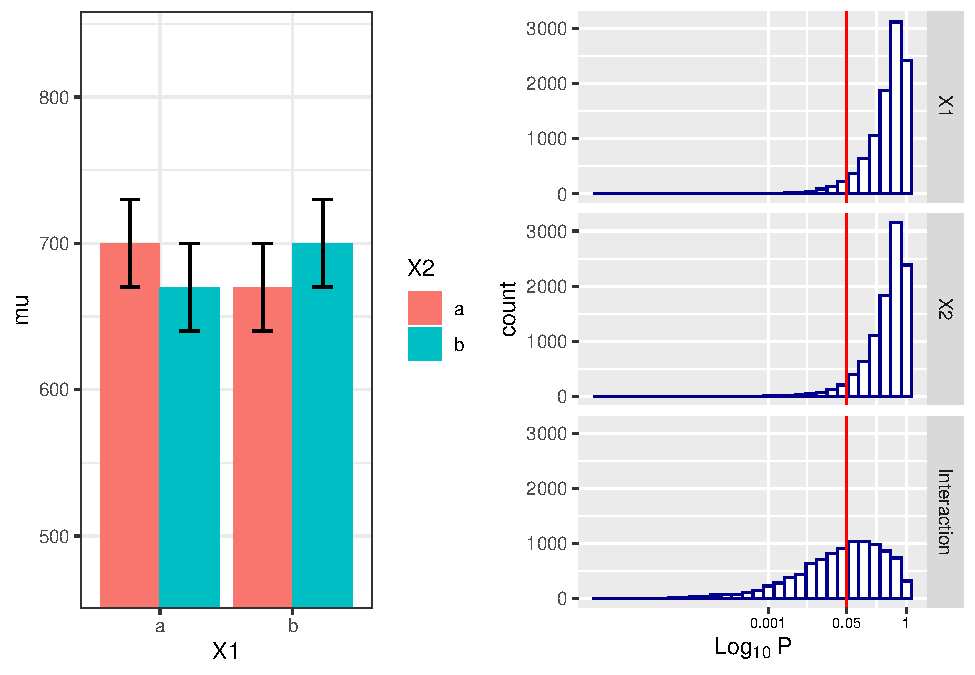
\includegraphics{SuperpowerValidation_files/figure-latex/unnamed-chunk-117-1.pdf}

We can reproduce this simulation:

\begin{Shaded}
\begin{Highlighting}[]
\CommentTok{\# true effects (in this case, a double dissociation)}
\NormalTok{mu }\OtherTok{=} \FunctionTok{c}\NormalTok{(}\DecValTok{700}\NormalTok{, }\DecValTok{670}\NormalTok{, }\DecValTok{670}\NormalTok{, }\DecValTok{700}\NormalTok{) }
\NormalTok{sigma }\OtherTok{=} \DecValTok{150}  \CommentTok{\# population standard deviation}
\NormalTok{n }\OtherTok{\textless{}{-}} \DecValTok{25}
\NormalTok{sd }\OtherTok{\textless{}{-}} \DecValTok{150}
\NormalTok{r }\OtherTok{\textless{}{-}} \FloatTok{0.75}
\NormalTok{string }\OtherTok{=} \StringTok{"2w*2w"}
\NormalTok{alpha\_level }\OtherTok{\textless{}{-}} \FloatTok{0.05}
\NormalTok{labelnames }\OtherTok{=} \FunctionTok{c}\NormalTok{(}\StringTok{"age"}\NormalTok{, }\StringTok{"old"}\NormalTok{, }\StringTok{"young"}\NormalTok{, }\StringTok{"color"}\NormalTok{, }\StringTok{"blue"}\NormalTok{, }\StringTok{"red"}\NormalTok{)}
\NormalTok{design\_result }\OtherTok{\textless{}{-}} \FunctionTok{ANOVA\_design}\NormalTok{(}\AttributeTok{design =}\NormalTok{ string,}
                              \AttributeTok{n =}\NormalTok{ n, }
                              \AttributeTok{mu =}\NormalTok{ mu, }
                              \AttributeTok{sd =}\NormalTok{ sd, }
                              \AttributeTok{r =}\NormalTok{ r, }
                              \AttributeTok{labelnames =}\NormalTok{ labelnames)}
\end{Highlighting}
\end{Shaded}

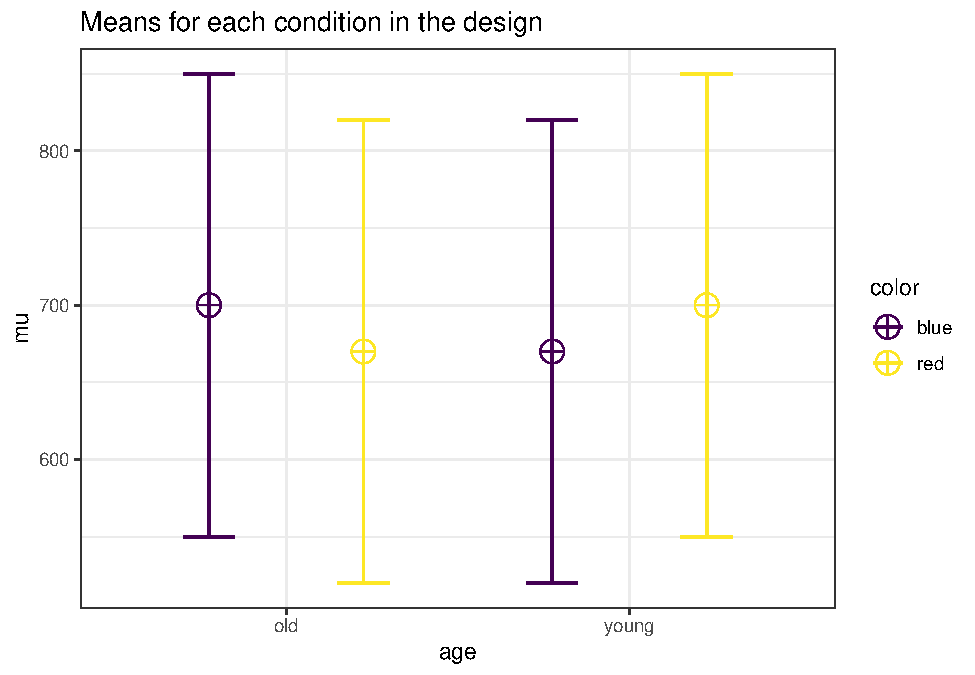
\includegraphics{SuperpowerValidation_files/figure-latex/unnamed-chunk-118-1.pdf}

\begin{Shaded}
\begin{Highlighting}[]
\NormalTok{simulation\_result }\OtherTok{\textless{}{-}} \FunctionTok{ANOVA\_power}\NormalTok{(design\_result, }
                                 \AttributeTok{alpha\_level =}\NormalTok{ alpha\_level, }
                                 \AttributeTok{nsims =}\NormalTok{ nsims,}
                                 \AttributeTok{verbose =} \ConstantTok{FALSE}\NormalTok{)}
\end{Highlighting}
\end{Shaded}

\begin{table}[!h]

\caption{\label{tab:unnamed-chunk-120}Simulated ANOVA Result}
\centering
\begin{tabular}[t]{l|r|r}
\hline
  & power & effect\_size\\
\hline
anova\_age & 4.78 & 0.0393606\\
\hline
anova\_color & 4.73 & 0.0388339\\
\hline
anova\_age:color & 48.65 & 0.1665309\\
\hline
\end{tabular}
\end{table}

\begin{Shaded}
\begin{Highlighting}[]
\NormalTok{exact\_result }\OtherTok{\textless{}{-}} \FunctionTok{ANOVA\_exact}\NormalTok{(design\_result,}
                            \AttributeTok{alpha\_level =}\NormalTok{ alpha\_level,}
                            \AttributeTok{verbose =} \ConstantTok{FALSE}\NormalTok{)}
\end{Highlighting}
\end{Shaded}

\begin{table}[!h]

\caption{\label{tab:unnamed-chunk-122}Exact ANOVA Result}
\centering
\begin{tabular}[t]{l|r|r|r|r}
\hline
  & power & partial\_eta\_squared & cohen\_f & non\_centrality\\
\hline
age & 5.00000 & 0.0000000 & 0.0000000 & 0\\
\hline
color & 5.00000 & 0.0000000 & 0.0000000 & 0\\
\hline
age:color & 48.40183 & 0.1428571 & 0.4082483 & 4\\
\hline
\end{tabular}
\end{table}

The simulations yield closely matching results.

\hypertarget{examine-variation-of-means-and-correlation}{%
\subsection{Examine variation of means and correlation}\label{examine-variation-of-means-and-correlation}}

\begin{Shaded}
\begin{Highlighting}[]
\CommentTok{\# define the parameters}
\CommentTok{\# true effects (in this case, a double dissociation)}
\NormalTok{mu }\OtherTok{=} \FunctionTok{c}\NormalTok{(}\DecValTok{700}\NormalTok{, }\DecValTok{670}\NormalTok{, }\DecValTok{690}\NormalTok{, }\DecValTok{750}\NormalTok{) }
\NormalTok{sigma }\OtherTok{=} \DecValTok{150}  \CommentTok{\# population standard deviation}
\NormalTok{rho }\OtherTok{=} \FloatTok{0.4} \CommentTok{\# correlation between repeated measures}
\NormalTok{nsubs }\OtherTok{=} \DecValTok{25} \CommentTok{\# how many subjects?}
\NormalTok{nsims }\OtherTok{=}\NormalTok{ nsims }\CommentTok{\# how many simulation replicates?}
 
\CommentTok{\# create 2 factors representing the 2 independent variables}
\NormalTok{cond }\OtherTok{=} \FunctionTok{data.frame}\NormalTok{(}\AttributeTok{X1 =} \FunctionTok{rep}\NormalTok{(}\FunctionTok{factor}\NormalTok{(letters[}\DecValTok{1}\SpecialCharTok{:}\DecValTok{2}\NormalTok{]), nsubs }\SpecialCharTok{*} \DecValTok{2}\NormalTok{),}
\AttributeTok{X2 =} \FunctionTok{rep}\NormalTok{(}\FunctionTok{factor}\NormalTok{(letters[}\DecValTok{1}\SpecialCharTok{:}\DecValTok{2}\NormalTok{]), nsubs, }\AttributeTok{each =} \DecValTok{2}\NormalTok{))}
 
\CommentTok{\# create a subjects factor}
\NormalTok{subject }\OtherTok{=} \FunctionTok{factor}\NormalTok{(}\FunctionTok{sort}\NormalTok{(}\FunctionTok{rep}\NormalTok{(}\DecValTok{1}\SpecialCharTok{:}\NormalTok{nsubs, }\DecValTok{4}\NormalTok{)))}
 
\CommentTok{\# combine above into the design matrix}
\NormalTok{dm }\OtherTok{=} \FunctionTok{data.frame}\NormalTok{(subject, cond)}
\end{Highlighting}
\end{Shaded}

Build Sigma: the population variance-covariance matrix

\begin{Shaded}
\begin{Highlighting}[]
\CommentTok{\# create k x k matrix populated with sigma}
\NormalTok{sigma.mat }\OtherTok{\textless{}{-}} \FunctionTok{rep}\NormalTok{(sigma, }\DecValTok{4}\NormalTok{)}
\NormalTok{S }\OtherTok{\textless{}{-}}
\FunctionTok{matrix}\NormalTok{(sigma.mat,}
\AttributeTok{ncol =} \FunctionTok{length}\NormalTok{(sigma.mat),}
\AttributeTok{nrow =} \FunctionTok{length}\NormalTok{(sigma.mat))}

\CommentTok{\# compute covariance between measures}
\NormalTok{Sigma }\OtherTok{\textless{}{-}} \FunctionTok{t}\NormalTok{(S) }\SpecialCharTok{*}\NormalTok{ S }\SpecialCharTok{*}\NormalTok{ rho}

\CommentTok{\# put the variances on the diagonal}
\FunctionTok{diag}\NormalTok{(Sigma) }\OtherTok{\textless{}{-}}\NormalTok{ sigma }\SpecialCharTok{\^{}} \DecValTok{2}  
\end{Highlighting}
\end{Shaded}

Run the simulation

\begin{Shaded}
\begin{Highlighting}[]
\CommentTok{\# stack \textquotesingle{}nsims\textquotesingle{} individual data frames into one large data frame}
\NormalTok{df }\OtherTok{=}\NormalTok{ dm[}\FunctionTok{rep}\NormalTok{(}\FunctionTok{seq\_len}\NormalTok{(}\FunctionTok{nrow}\NormalTok{(dm)), nsims), ]}
 
\CommentTok{\# add an index column to track the simulation run}
\NormalTok{df}\SpecialCharTok{$}\NormalTok{simID }\OtherTok{=} \FunctionTok{sort}\NormalTok{(}\FunctionTok{rep}\NormalTok{(}\FunctionTok{seq\_len}\NormalTok{(nsims), }\FunctionTok{nrow}\NormalTok{(dm)))}
 
\CommentTok{\# sample the observed data from a multivariate normal distribution}
\CommentTok{\# using MASS::mvrnorm with the mu and Sigma created earlier}
\CommentTok{\# and bind to the existing df}
 

\NormalTok{make.y }\OtherTok{=} \FunctionTok{expression}\NormalTok{(}\FunctionTok{as.vector}\NormalTok{(}\FunctionTok{t}\NormalTok{(}\FunctionTok{mvrnorm}\NormalTok{(nsubs, mu, Sigma))))}
\NormalTok{df}\SpecialCharTok{$}\NormalTok{y }\OtherTok{=} \FunctionTok{as.vector}\NormalTok{(}\FunctionTok{replicate}\NormalTok{(nsims, }\FunctionTok{eval}\NormalTok{(make.y)))             }
 
\CommentTok{\# use do(), the general purpose complement to the specialized data }
\CommentTok{\# manipulation functions available in dplyr, to run the ANOVA on}
\CommentTok{\# each section of the grouped data frame created by group\_by}
 

\NormalTok{mods }\OtherTok{\textless{}{-}}\NormalTok{ df }\SpecialCharTok{\%\textgreater{}\%}
  \FunctionTok{group\_by}\NormalTok{(simID) }\SpecialCharTok{\%\textgreater{}\%}
  \FunctionTok{do}\NormalTok{(}\AttributeTok{model =} \FunctionTok{aov}\NormalTok{(y }\SpecialCharTok{\textasciitilde{}}\NormalTok{ X1 }\SpecialCharTok{*}\NormalTok{ X2 }\SpecialCharTok{+} \FunctionTok{Error}\NormalTok{(subject }\SpecialCharTok{/}\NormalTok{ (X1 }\SpecialCharTok{*}\NormalTok{ X2)), }
                 \AttributeTok{qr =} \ConstantTok{FALSE}\NormalTok{, }\AttributeTok{data =}\NormalTok{ .))}
  
  \CommentTok{\# extract p{-}values for each effect and store in a data frame}
\NormalTok{  p\_val\_2 }\OtherTok{=} \FunctionTok{data.frame}\NormalTok{(mods }\SpecialCharTok{\%\textgreater{}\%} 
                   \FunctionTok{do}\NormalTok{(}\FunctionTok{as.data.frame}\NormalTok{(}\FunctionTok{tidy}\NormalTok{(.}\SpecialCharTok{$}\NormalTok{model[[}\DecValTok{3}\NormalTok{]])}\SpecialCharTok{$}\NormalTok{p.value[}\DecValTok{1}\NormalTok{])),}
\NormalTok{  mods }\SpecialCharTok{\%\textgreater{}\%} \FunctionTok{do}\NormalTok{(}\FunctionTok{as.data.frame}\NormalTok{(}\FunctionTok{tidy}\NormalTok{(.}\SpecialCharTok{$}\NormalTok{model[[}\DecValTok{4}\NormalTok{]])}\SpecialCharTok{$}\NormalTok{p.value[}\DecValTok{1}\NormalTok{])),}
\NormalTok{  mods }\SpecialCharTok{\%\textgreater{}\%} \FunctionTok{do}\NormalTok{(}\FunctionTok{as.data.frame}\NormalTok{(}\FunctionTok{tidy}\NormalTok{(.}\SpecialCharTok{$}\NormalTok{model[[}\DecValTok{5}\NormalTok{]])}\SpecialCharTok{$}\NormalTok{p.value[}\DecValTok{1}\NormalTok{])))}
  \FunctionTok{colnames}\NormalTok{(p\_val\_2) }\OtherTok{=} \FunctionTok{c}\NormalTok{(}\StringTok{\textquotesingle{}X1\textquotesingle{}}\NormalTok{, }\StringTok{\textquotesingle{}X2\textquotesingle{}}\NormalTok{, }\StringTok{\textquotesingle{}Interaction\textquotesingle{}}\NormalTok{)}
\end{Highlighting}
\end{Shaded}

The empirical power is easy to compute, it's just the proportion of simulation runs where p \textless. 05.

\begin{Shaded}
\begin{Highlighting}[]
\NormalTok{power.res }\OtherTok{=} \FunctionTok{apply}\NormalTok{(}\FunctionTok{as.matrix}\NormalTok{(p\_val\_2), }\DecValTok{2}\NormalTok{, }
  \ControlFlowTok{function}\NormalTok{(x) }\FunctionTok{round}\NormalTok{(}\FunctionTok{mean}\NormalTok{(}\FunctionTok{ifelse}\NormalTok{(x }\SpecialCharTok{\textless{}}\NormalTok{ .}\DecValTok{05}\NormalTok{, }\DecValTok{1}\NormalTok{, }\DecValTok{0}\NormalTok{) }\SpecialCharTok{*} \DecValTok{100}\NormalTok{),}\DecValTok{2}\NormalTok{))}
\NormalTok{power.res}
\end{Highlighting}
\end{Shaded}

\begin{verbatim}
##          X1          X2 Interaction 
##        9.64       30.44       45.95
\end{verbatim}

Visualize the distributions of \emph{p}-values

\begin{Shaded}
\begin{Highlighting}[]
\NormalTok{means }\OtherTok{=} \FunctionTok{data.frame}\NormalTok{(cond[}\DecValTok{1}\SpecialCharTok{:}\DecValTok{4}\NormalTok{,], mu, }\AttributeTok{SE =}\NormalTok{ sigma }\SpecialCharTok{/} \FunctionTok{sqrt}\NormalTok{(nsubs))}
\NormalTok{plt1 }\OtherTok{=} \FunctionTok{ggplot}\NormalTok{(means, }\FunctionTok{aes}\NormalTok{(}\AttributeTok{y =}\NormalTok{ mu, }\AttributeTok{x =}\NormalTok{ X1, }\AttributeTok{fill =}\NormalTok{ X2)) }\SpecialCharTok{+}
\FunctionTok{geom\_bar}\NormalTok{(}\AttributeTok{position =} \FunctionTok{position\_dodge}\NormalTok{(), }\AttributeTok{stat =} \StringTok{"identity"}\NormalTok{) }\SpecialCharTok{+}
\FunctionTok{geom\_errorbar}\NormalTok{(}
\FunctionTok{aes}\NormalTok{(}\AttributeTok{ymin =}\NormalTok{ mu }\SpecialCharTok{{-}}\NormalTok{ SE, }\AttributeTok{ymax =}\NormalTok{ mu }\SpecialCharTok{+}\NormalTok{ SE),}
\AttributeTok{position =} \FunctionTok{position\_dodge}\NormalTok{(}\AttributeTok{width =} \FloatTok{0.9}\NormalTok{),}
\AttributeTok{size =}\NormalTok{ .}\DecValTok{6}\NormalTok{,}
\AttributeTok{width =}\NormalTok{ .}\DecValTok{3}
\NormalTok{) }\SpecialCharTok{+}
\FunctionTok{coord\_cartesian}\NormalTok{(}\AttributeTok{ylim =} \FunctionTok{c}\NormalTok{((.}\DecValTok{7} \SpecialCharTok{*} \FunctionTok{min}\NormalTok{(mu)), }\FloatTok{1.2} \SpecialCharTok{*} \FunctionTok{max}\NormalTok{(mu))) }\SpecialCharTok{+}
\FunctionTok{theme\_bw}\NormalTok{()}
 
\CommentTok{\# melt the data into a ggplot friendly \textquotesingle{}long\textquotesingle{} format}

\NormalTok{plotData }\OtherTok{\textless{}{-}} \FunctionTok{melt}\NormalTok{(p\_val\_2, }\AttributeTok{value.name =} \StringTok{\textquotesingle{}p\textquotesingle{}}\NormalTok{)}
 
\CommentTok{\# plot each of the p{-}value distributions on a log scale}
\FunctionTok{options}\NormalTok{(}\AttributeTok{scipen =} \DecValTok{999}\NormalTok{) }\CommentTok{\# \textquotesingle{}turn off\textquotesingle{} scientific notation}
\NormalTok{plt2 }\OtherTok{=} \FunctionTok{ggplot}\NormalTok{(plotData, }\FunctionTok{aes}\NormalTok{(}\AttributeTok{x =}\NormalTok{ p)) }\SpecialCharTok{+}
\FunctionTok{scale\_x\_log10}\NormalTok{(}\AttributeTok{breaks =} \FunctionTok{c}\NormalTok{(}\DecValTok{1}\NormalTok{, }\FloatTok{0.05}\NormalTok{, }\FloatTok{0.001}\NormalTok{),}
\AttributeTok{labels =} \FunctionTok{c}\NormalTok{(}\DecValTok{1}\NormalTok{, }\FloatTok{0.05}\NormalTok{, }\FloatTok{0.001}\NormalTok{)) }\SpecialCharTok{+}
\FunctionTok{geom\_histogram}\NormalTok{(}\AttributeTok{colour =} \StringTok{"darkblue"}\NormalTok{, }\AttributeTok{fill =} \StringTok{"white"}\NormalTok{) }\SpecialCharTok{+}
\FunctionTok{geom\_vline}\NormalTok{(}\AttributeTok{xintercept =} \FloatTok{0.05}\NormalTok{, }\AttributeTok{colour =} \StringTok{\textquotesingle{}red\textquotesingle{}}\NormalTok{) }\SpecialCharTok{+}
\FunctionTok{facet\_grid}\NormalTok{(variable }\SpecialCharTok{\textasciitilde{}}\NormalTok{ .) }\SpecialCharTok{+}
\FunctionTok{labs}\NormalTok{(}\AttributeTok{x =} \FunctionTok{expression}\NormalTok{(Log[}\DecValTok{10}\NormalTok{] }\SpecialCharTok{\textasciitilde{}}\NormalTok{ P)) }\SpecialCharTok{+}
\FunctionTok{theme}\NormalTok{(}\AttributeTok{axis.text.x =} \FunctionTok{element\_text}\NormalTok{(}\AttributeTok{color =} \StringTok{\textquotesingle{}black\textquotesingle{}}\NormalTok{, }\AttributeTok{size =} \DecValTok{7}\NormalTok{))}

\CommentTok{\# arrange plots side by side and print}
\FunctionTok{grid.arrange}\NormalTok{(plt1, plt2, }\AttributeTok{nrow =} \DecValTok{1}\NormalTok{)}
\end{Highlighting}
\end{Shaded}

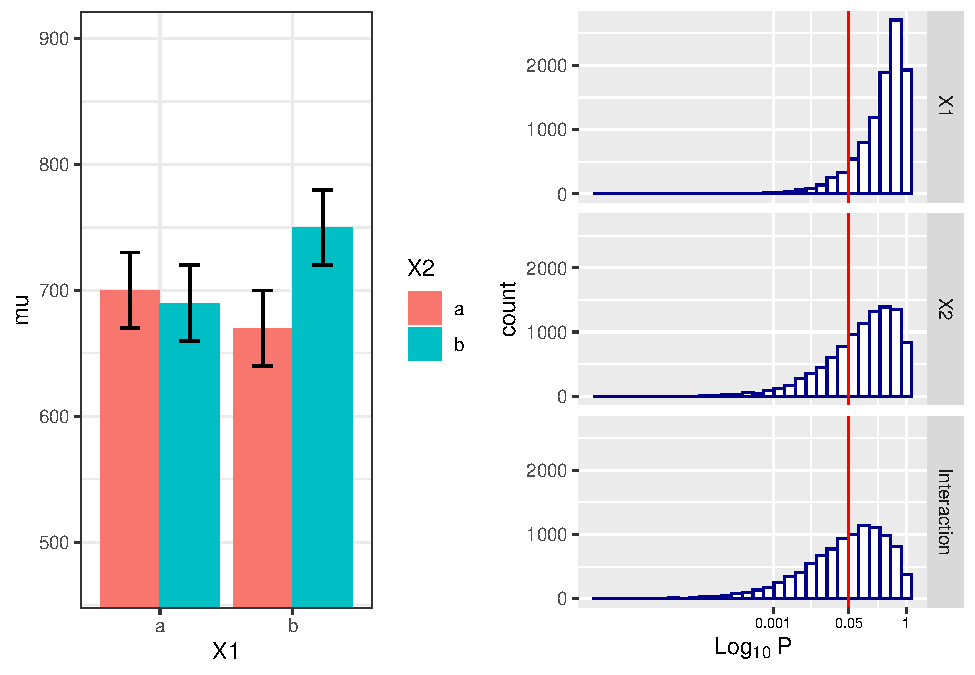
\includegraphics{SuperpowerValidation_files/figure-latex/unnamed-chunk-127-1.pdf}

We can reproduce this simulation:

\begin{Shaded}
\begin{Highlighting}[]
\CommentTok{\# true effects (in this case, a double dissociation)}
\NormalTok{mu }\OtherTok{=} \FunctionTok{c}\NormalTok{(}\DecValTok{700}\NormalTok{, }\DecValTok{670}\NormalTok{, }\DecValTok{690}\NormalTok{, }\DecValTok{750}\NormalTok{) }
\NormalTok{sigma }\OtherTok{=} \DecValTok{150}  \CommentTok{\# population standard deviation}
\NormalTok{n }\OtherTok{\textless{}{-}} \DecValTok{25}
\NormalTok{sd }\OtherTok{\textless{}{-}} \DecValTok{150}
\NormalTok{r }\OtherTok{\textless{}{-}} \FloatTok{0.4}
\NormalTok{string }\OtherTok{=} \StringTok{"2w*2w"}
\NormalTok{alpha\_level }\OtherTok{\textless{}{-}} \FloatTok{0.05}
\NormalTok{labelnames }\OtherTok{=} \FunctionTok{c}\NormalTok{(}\StringTok{"AGE"}\NormalTok{, }\StringTok{"old"}\NormalTok{, }\StringTok{"young"}\NormalTok{, }
               \StringTok{"COLOR"}\NormalTok{, }\StringTok{"blue"}\NormalTok{, }\StringTok{"red"}\NormalTok{)}

\NormalTok{design\_result }\OtherTok{\textless{}{-}} \FunctionTok{ANOVA\_design}\NormalTok{(}\AttributeTok{design =}\NormalTok{ string,}
                              \AttributeTok{n =}\NormalTok{ n, }
                              \AttributeTok{mu =}\NormalTok{ mu, }
                              \AttributeTok{sd =}\NormalTok{ sd, }
                              \AttributeTok{r =}\NormalTok{ r, }
                              \AttributeTok{labelnames =}\NormalTok{ labelnames)}
\end{Highlighting}
\end{Shaded}

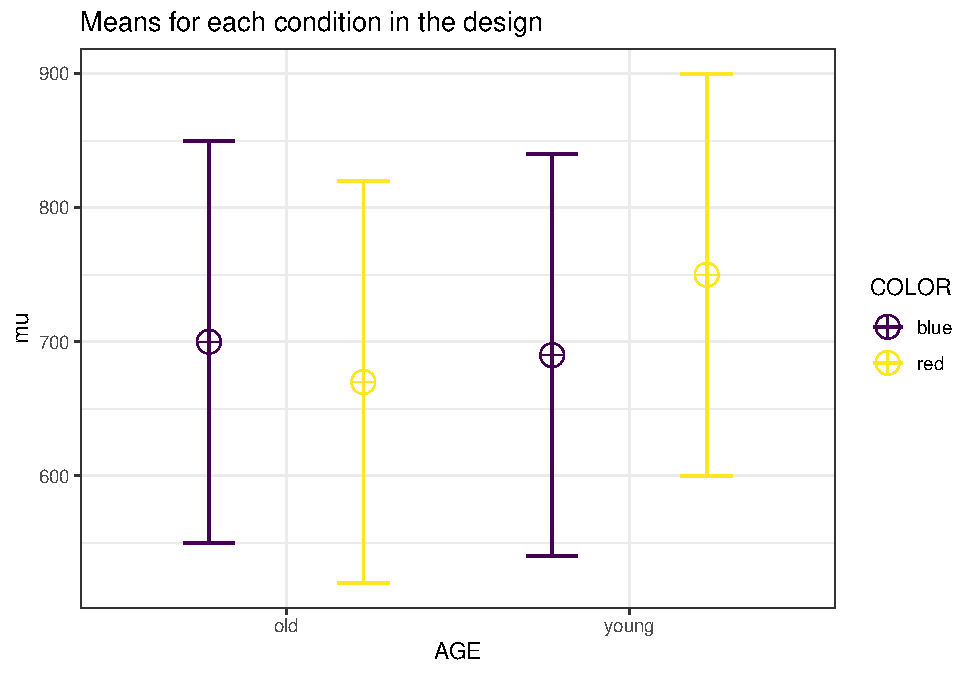
\includegraphics{SuperpowerValidation_files/figure-latex/unnamed-chunk-128-1.pdf}

\begin{Shaded}
\begin{Highlighting}[]
\NormalTok{simulation\_result }\OtherTok{\textless{}{-}} \FunctionTok{ANOVA\_power}\NormalTok{(design\_result, }
                                 \AttributeTok{alpha\_level =} \FloatTok{0.05}\NormalTok{, }
                                 \AttributeTok{nsims =}\NormalTok{ nsims)}
\end{Highlighting}
\end{Shaded}

\begin{table}[!h]

\caption{\label{tab:unnamed-chunk-130}Simulated ANOVA Result}
\centering
\begin{tabular}[t]{l|r|r}
\hline
  & power & effect\_size\\
\hline
anova\_AGE & 30.05 & 0.1143297\\
\hline
anova\_COLOR & 9.45 & 0.0551819\\
\hline
anova\_AGE:COLOR & 46.26 & 0.1591529\\
\hline
\end{tabular}
\end{table}

\begin{Shaded}
\begin{Highlighting}[]
\NormalTok{exact\_result }\OtherTok{\textless{}{-}} \FunctionTok{ANOVA\_exact}\NormalTok{(design\_result, }\AttributeTok{alpha\_level =}\NormalTok{ alpha\_level)}
\end{Highlighting}
\end{Shaded}

\begin{verbatim}
## Power and Effect sizes for ANOVA tests
##             power partial_eta_squared cohen_f non_centrality
## AGE       30.4009              0.0864  0.3074         2.2685
## COLOR      9.5071              0.0171  0.1318         0.4167
## AGE:COLOR 45.9803              0.1351  0.3953         3.7500
## 
## Power and Effect sizes for pairwise comparisons (t-tests)
##                                            power effect_size
## p_AGE_old_COLOR_blue_AGE_old_COLOR_red     14.16       -0.18
## p_AGE_old_COLOR_blue_AGE_young_COLOR_blue   5.98       -0.06
## p_AGE_old_COLOR_blue_AGE_young_COLOR_red   30.91        0.30
## p_AGE_old_COLOR_red_AGE_young_COLOR_blue    9.00        0.12
## p_AGE_old_COLOR_red_AGE_young_COLOR_red    64.66        0.49
## p_AGE_young_COLOR_blue_AGE_young_COLOR_red 41.80        0.37
\end{verbatim}

\begin{table}[!h]

\caption{\label{tab:unnamed-chunk-132}Exact ANOVA Result}
\centering
\begin{tabular}[t]{l|r|r|r|r}
\hline
  & power & partial\_eta\_squared & cohen\_f & non\_centrality\\
\hline
AGE & 30.400885 & 0.0863588 & 0.3074437 & 2.2685185\\
\hline
COLOR & 9.507147 & 0.0170648 & 0.1317616 & 0.4166667\\
\hline
AGE:COLOR & 45.980305 & 0.1351351 & 0.3952847 & 3.7500000\\
\hline
\end{tabular}
\end{table}

\hypertarget{part-5}{%
\section{Part 5}\label{part-5}}

\textbf{Credit for the non-centrality parameter for the interaction goes to Andrew Vigotsky}

\hypertarget{x2-anova-within-design}{%
\subsection{2x2 ANOVA, within design}\label{x2-anova-within-design}}

\citet{potvin2000statistical} simulate a wide range of repeated measure designs. They give an example of a 3x3 design, with the following correlation matrix:

\includegraphics{screenshots/PS2000.png}

Variances were set to 1 (so all covariance matrices in their simulations were identical). In this specific example, the white fields are related to the correlation for the A main effect (these cells have the same level for B, but different levels of A). The grey cells are related to the main effect of B (the cells have the same level of A, but different levels of B). Finally, the black cells are related to the AxB interaction (they have different levels of A and B). The diagonal (all 1) relate to cells with the same levels of A and B.

\citet{potvin2000statistical} examine power for 2x2 within ANOVA designs and develop approximations of the error variance. For a design with 2 within factors (A and B) these are:

For the main effect of A:
\(\sigma _ { e } ^ { 2 } = \sigma ^ { 2 } ( 1 - \overline { \rho } _ { A } ) + \sigma ^ { 2 } ( q - 1 ) ( \overline { \rho } _ { B } - \overline { \rho } _ { AB } )\)

For the main effectof B:
\(\sigma _ { e } ^ { 2 } = \sigma ^ { 2 } ( 1 - \overline { \rho } _ { B } ) + \sigma ^ { 2 } ( p - 1 ) ( \overline { \rho } _ { A } - \overline { \rho } _ { A B } )\)

For the interaction between A and B:
\(\sigma _ { e } ^ { 2 } = \sigma ^ { 2 } ( 1 - \rho _ { \max } ) - \sigma ^ { 2 } ( \overline { \rho } _ { \min } - \overline { \rho } _ { AB } )\)

Let's now compare the formulas in \citet{potvin2000statistical} with \texttt{Superpower} with a simple scenario.

\begin{Shaded}
\begin{Highlighting}[]
\NormalTok{mu }\OtherTok{=} \FunctionTok{c}\NormalTok{(}\DecValTok{2}\NormalTok{,}\DecValTok{1}\NormalTok{,}\DecValTok{4}\NormalTok{,}\DecValTok{2}\NormalTok{) }
\NormalTok{n }\OtherTok{\textless{}{-}} \DecValTok{20}
\NormalTok{sd }\OtherTok{\textless{}{-}} \DecValTok{5}
\NormalTok{r }\OtherTok{\textless{}{-}}\NormalTok{ .}\DecValTok{77}
\NormalTok{string }\OtherTok{=} \StringTok{"2w*2w"}
\NormalTok{alpha\_level }\OtherTok{\textless{}{-}} \FloatTok{0.05}


\NormalTok{design\_result }\OtherTok{\textless{}{-}} \FunctionTok{ANOVA\_design}\NormalTok{(}\AttributeTok{design =}\NormalTok{ string,}
                              \AttributeTok{n =}\NormalTok{ n, }
                              \AttributeTok{mu =}\NormalTok{ mu, }
                              \AttributeTok{sd =}\NormalTok{ sd, }
                              \AttributeTok{r =}\NormalTok{ r, }
                              \AttributeTok{labelnames =}\NormalTok{ labelnames,}
                              \AttributeTok{plot =} \ConstantTok{TRUE}\NormalTok{)}
\end{Highlighting}
\end{Shaded}

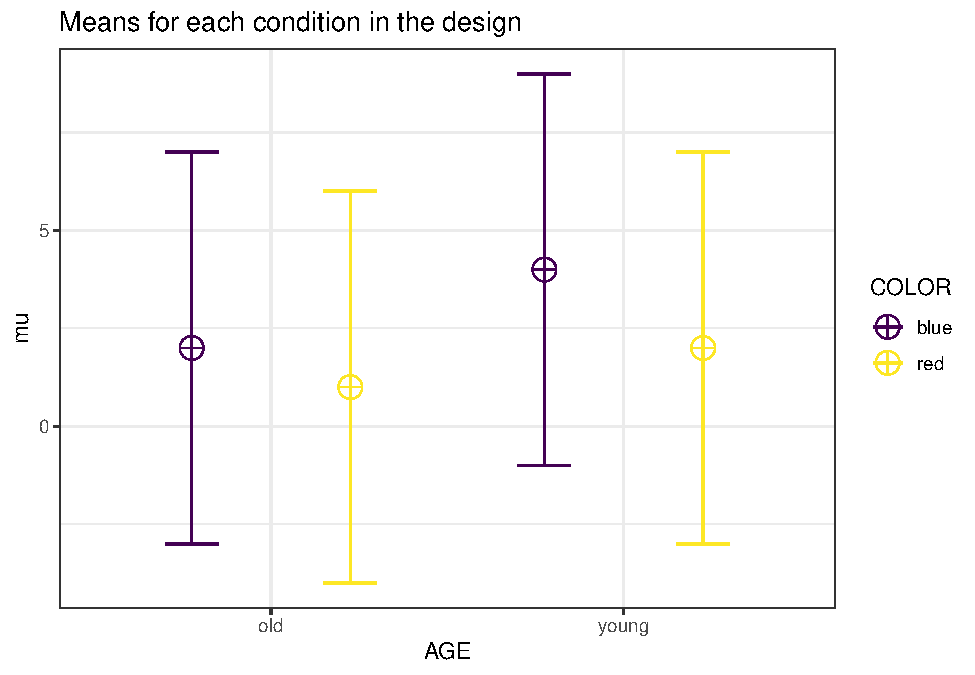
\includegraphics{SuperpowerValidation_files/figure-latex/unnamed-chunk-133-1.pdf}

\begin{Shaded}
\begin{Highlighting}[]
\NormalTok{design\_result}\SpecialCharTok{$}\NormalTok{cor\_mat}
\end{Highlighting}
\end{Shaded}

\begin{verbatim}
##            old_blue old_red young_blue young_red
## old_blue       1.00    0.77       0.77      0.77
## old_red        0.77    1.00       0.77      0.77
## young_blue     0.77    0.77       1.00      0.77
## young_red      0.77    0.77       0.77      1.00
\end{verbatim}

\begin{Shaded}
\begin{Highlighting}[]
\NormalTok{exact\_result }\OtherTok{\textless{}{-}} \FunctionTok{ANOVA\_exact}\NormalTok{(design\_result,}
                            \AttributeTok{alpha\_level =}\NormalTok{ alpha\_level,}
                            \AttributeTok{verbose =} \ConstantTok{FALSE}\NormalTok{)}
\end{Highlighting}
\end{Shaded}

\begin{table}[!h]

\caption{\label{tab:unnamed-chunk-135}Exact ANOVA Result}
\centering
\begin{tabular}[t]{l|r|r|r|r}
\hline
  & power & partial\_eta\_squared & cohen\_f & non\_centrality\\
\hline
AGE & 75.61412 & 0.2917342 & 0.6417938 & 7.8260870\\
\hline
COLOR & 75.61412 & 0.2917342 & 0.6417938 & 7.8260870\\
\hline
AGE:COLOR & 14.36376 & 0.0437637 & 0.2139313 & 0.8695652\\
\hline
\end{tabular}
\end{table}

Further, as we use the analytical solution below, the variance components should be equal to the corresponding MSE from the \texttt{ANOVA\_exact} produced \texttt{anova\_table} object.

\begin{Shaded}
\begin{Highlighting}[]
\NormalTok{exact\_result}\SpecialCharTok{$}\NormalTok{aov\_result}\SpecialCharTok{$}\NormalTok{anova\_table}
\end{Highlighting}
\end{Shaded}

\begin{verbatim}
## Anova Table (Type 3 tests)
## 
## Response: y
##           num Df den Df  MSE      F      pes  Pr(>F)  
## AGE            1     19 5.75 7.8261 0.291734 0.01149 *
## COLOR          1     19 5.75 7.8261 0.291734 0.01149 *
## AGE:COLOR      1     19 5.75 0.8696 0.043764 0.36278  
## ---
## Signif. codes:  0 '***' 0.001 '**' 0.01 '*' 0.05 '.' 0.1 ' ' 1
\end{verbatim}

We can try to use the formula in \citet{potvin2000statistical}.

\begin{Shaded}
\begin{Highlighting}[]
\NormalTok{k }\OtherTok{\textless{}{-}} \DecValTok{1} \CommentTok{\#one group (because all factors are within)}

\NormalTok{rho\_A }\OtherTok{\textless{}{-}}\NormalTok{ .}\DecValTok{77} \CommentTok{\#mean r for factor A}

\NormalTok{rho\_B }\OtherTok{\textless{}{-}}\NormalTok{ .}\DecValTok{77} \CommentTok{\#mean r for factor B}

\NormalTok{rho\_AB }\OtherTok{\textless{}{-}}\NormalTok{ .}\DecValTok{77} \CommentTok{\#mean r for factor AB}

\NormalTok{alpha }\OtherTok{\textless{}{-}} \FloatTok{0.05}

\NormalTok{sigma }\OtherTok{\textless{}{-}}\NormalTok{ sd}

\NormalTok{m\_A }\OtherTok{\textless{}{-}} \DecValTok{2} \CommentTok{\#levels factor A}

\NormalTok{variance\_e\_A }\OtherTok{\textless{}{-}}\NormalTok{ (sigma}\SpecialCharTok{\^{}}\DecValTok{2} \SpecialCharTok{*}\NormalTok{ (}\DecValTok{1} \SpecialCharTok{{-}}\NormalTok{ rho\_A) }\SpecialCharTok{+} 
\NormalTok{  sigma}\SpecialCharTok{\^{}}\DecValTok{2} \SpecialCharTok{*}\NormalTok{ (m\_A }\SpecialCharTok{{-}} \DecValTok{1}\NormalTok{) }\SpecialCharTok{*}\NormalTok{ (rho\_B }\SpecialCharTok{{-}}\NormalTok{ rho\_AB) )}
\CommentTok{\#Variance A}
\NormalTok{variance\_e\_A}
\end{Highlighting}
\end{Shaded}

\begin{verbatim}
## [1] 5.75
\end{verbatim}

\begin{Shaded}
\begin{Highlighting}[]
\NormalTok{m\_B }\OtherTok{\textless{}{-}} \DecValTok{2} \CommentTok{\#levels factor B}

\NormalTok{variance\_e\_B }\OtherTok{\textless{}{-}}\NormalTok{ sigma}\SpecialCharTok{\^{}}\DecValTok{2} \SpecialCharTok{*}\NormalTok{ (}\DecValTok{1} \SpecialCharTok{{-}}\NormalTok{ rho\_B) }\SpecialCharTok{+} 
\NormalTok{  sigma}\SpecialCharTok{\^{}}\DecValTok{2} \SpecialCharTok{*}\NormalTok{ (m\_B }\SpecialCharTok{{-}} \DecValTok{1}\NormalTok{) }\SpecialCharTok{*}\NormalTok{ (rho\_A }\SpecialCharTok{{-}}\NormalTok{ rho\_AB)}
\CommentTok{\#Variance B}
\NormalTok{variance\_e\_B}
\end{Highlighting}
\end{Shaded}

\begin{verbatim}
## [1] 5.75
\end{verbatim}

\begin{Shaded}
\begin{Highlighting}[]
\NormalTok{variance\_e\_AB }\OtherTok{\textless{}{-}}
\NormalTok{  (sigma }\SpecialCharTok{\^{}} \DecValTok{2} \SpecialCharTok{*}\NormalTok{ (}\DecValTok{1} \SpecialCharTok{{-}} \FunctionTok{max}\NormalTok{(rho\_A, rho\_B)) }\SpecialCharTok{{-}} 
\NormalTok{     sigma }\SpecialCharTok{\^{}} \DecValTok{2} \SpecialCharTok{*}\NormalTok{ (}\FunctionTok{min}\NormalTok{(rho\_A,rho\_B) }\SpecialCharTok{{-}}\NormalTok{ rho\_AB)) }
\CommentTok{\#Variance AB}
\NormalTok{variance\_e\_AB}
\end{Highlighting}
\end{Shaded}

\begin{verbatim}
## [1] 5.75
\end{verbatim}

\begin{Shaded}
\begin{Highlighting}[]
\CommentTok{\#Create a mean matrix}
\NormalTok{mean\_mat }\OtherTok{\textless{}{-}} \FunctionTok{t}\NormalTok{(}\FunctionTok{matrix}\NormalTok{(mu, }\AttributeTok{nrow =}\NormalTok{ m\_B,}\AttributeTok{ncol =}\NormalTok{ m\_A)) }
\NormalTok{mean\_mat}
\end{Highlighting}
\end{Shaded}

\begin{verbatim}
##      [,1] [,2]
## [1,]    2    1
## [2,]    4    2
\end{verbatim}

\begin{Shaded}
\begin{Highlighting}[]
\CommentTok{\# Potvin \& Schutz, 2000, formula 2, p. 348}
\CommentTok{\# For main effect A}
\NormalTok{lambda\_A }\OtherTok{\textless{}{-}}
\NormalTok{  (n }\SpecialCharTok{*}\NormalTok{ m\_A }\SpecialCharTok{*} \FunctionTok{sum}\NormalTok{((}\FunctionTok{rowMeans}\NormalTok{(mean\_mat) }\SpecialCharTok{{-}} 
                   \FunctionTok{mean}\NormalTok{(}\FunctionTok{rowMeans}\NormalTok{(mean\_mat))) }\SpecialCharTok{\^{}} \DecValTok{2}\NormalTok{) ) }\SpecialCharTok{/}\NormalTok{ variance\_e\_A}
\NormalTok{  lambda\_A}
\end{Highlighting}
\end{Shaded}

\begin{verbatim}
## [1] 7.826087
\end{verbatim}

\begin{Shaded}
\begin{Highlighting}[]
\CommentTok{\#calculate degrees of freedom 1 {-} ignoring the sphericity correction}
\NormalTok{df1 }\OtherTok{\textless{}{-}}\NormalTok{ (m\_A }\SpecialCharTok{{-}} \DecValTok{1}\NormalTok{) }

\NormalTok{df2 }\OtherTok{\textless{}{-}}\NormalTok{ (n }\SpecialCharTok{{-}}\NormalTok{ k) }\SpecialCharTok{*}\NormalTok{ (m\_A }\SpecialCharTok{{-}} \DecValTok{1}\NormalTok{) }\CommentTok{\#calculate degrees of freedom 2}

\NormalTok{F\_critical }\OtherTok{\textless{}{-}} \FunctionTok{qf}\NormalTok{(alpha, }\CommentTok{\# critical F{-}vaue}
\NormalTok{                 df1,}
\NormalTok{                 df2, }
                 \AttributeTok{lower.tail =} \ConstantTok{FALSE}\NormalTok{) }

\NormalTok{pow\_A }\OtherTok{\textless{}{-}} \FunctionTok{pf}\NormalTok{(}\FunctionTok{qf}\NormalTok{(alpha, }\CommentTok{\#power }
\NormalTok{             df1, }
\NormalTok{             df2, }
             \AttributeTok{lower.tail =} \ConstantTok{FALSE}\NormalTok{), }
\NormalTok{          df1, }
\NormalTok{          df2, }
\NormalTok{          lambda\_A, }
          \AttributeTok{lower.tail =} \ConstantTok{FALSE}\NormalTok{)}
\NormalTok{pow\_A}\SpecialCharTok{*}\DecValTok{100}
\end{Highlighting}
\end{Shaded}

\begin{verbatim}
## [1] 75.61412
\end{verbatim}

\begin{Shaded}
\begin{Highlighting}[]
\NormalTok{lambda\_B }\OtherTok{\textless{}{-}}
\NormalTok{  n }\SpecialCharTok{*}\NormalTok{ m\_B }\SpecialCharTok{*} \FunctionTok{sum}\NormalTok{((}\FunctionTok{colMeans}\NormalTok{(mean\_mat) }\SpecialCharTok{{-}} 
                   \FunctionTok{mean}\NormalTok{(}\FunctionTok{colMeans}\NormalTok{(mean\_mat))) }\SpecialCharTok{\^{}} \DecValTok{2}\NormalTok{) }\SpecialCharTok{/}\NormalTok{ variance\_e\_B }
\NormalTok{lambda\_B}
\end{Highlighting}
\end{Shaded}

\begin{verbatim}
## [1] 7.826087
\end{verbatim}

\begin{Shaded}
\begin{Highlighting}[]
\NormalTok{df1 }\OtherTok{\textless{}{-}}\NormalTok{ (m\_B }\SpecialCharTok{{-}} \DecValTok{1}\NormalTok{) }\CommentTok{\#calculate degrees of freedom 1}

\NormalTok{df2 }\OtherTok{\textless{}{-}}\NormalTok{ (n }\SpecialCharTok{{-}}\NormalTok{ k) }\SpecialCharTok{*}\NormalTok{ (m\_B }\SpecialCharTok{{-}} \DecValTok{1}\NormalTok{) }\CommentTok{\#calculate degrees of freedom 2}

\NormalTok{F\_critical }\OtherTok{\textless{}{-}} \FunctionTok{qf}\NormalTok{(alpha, }\CommentTok{\# critical F{-}vaue}
\NormalTok{                 df1,}
\NormalTok{                 df2,}
                 \AttributeTok{lower.tail =} \ConstantTok{FALSE}\NormalTok{) }

\NormalTok{pow\_B }\OtherTok{\textless{}{-}} \FunctionTok{pf}\NormalTok{(}\FunctionTok{qf}\NormalTok{(alpha, }\CommentTok{\#power }
\NormalTok{             df1, }
\NormalTok{             df2, }
             \AttributeTok{lower.tail =} \ConstantTok{FALSE}\NormalTok{), }
\NormalTok{          df1, }
\NormalTok{          df2, }
\NormalTok{          lambda\_B, }
          \AttributeTok{lower.tail =} \ConstantTok{FALSE}\NormalTok{)}


\NormalTok{pow\_B}\SpecialCharTok{*}\DecValTok{100}
\end{Highlighting}
\end{Shaded}

\begin{verbatim}
## [1] 75.61412
\end{verbatim}

\begin{Shaded}
\begin{Highlighting}[]
\CommentTok{\#Peform double summation courtesy of Andrew Vigotsky}
\NormalTok{term }\OtherTok{\textless{}{-}} \DecValTok{0}
\ControlFlowTok{for}\NormalTok{ (i }\ControlFlowTok{in} \DecValTok{1}\SpecialCharTok{:}\FunctionTok{nrow}\NormalTok{(mean\_mat)) \{}
  \ControlFlowTok{for}\NormalTok{ (j }\ControlFlowTok{in} \DecValTok{1}\SpecialCharTok{:}\FunctionTok{ncol}\NormalTok{(mean\_mat)) \{}
\NormalTok{    term }\OtherTok{\textless{}{-}}\NormalTok{ (term }\SpecialCharTok{+}\NormalTok{ (mean\_mat[i,j] }\SpecialCharTok{{-}} 
                       \FunctionTok{mean}\NormalTok{(mean\_mat[i,]) }\SpecialCharTok{{-}} 
                       \FunctionTok{mean}\NormalTok{(mean\_mat[,j]) }\SpecialCharTok{+} \FunctionTok{mean}\NormalTok{(mean\_mat))}\SpecialCharTok{\^{}}\DecValTok{2}\NormalTok{)}
\NormalTok{  \}}
\NormalTok{\}}
\NormalTok{term}
\end{Highlighting}
\end{Shaded}

\begin{verbatim}
## [1] 0.25
\end{verbatim}

\begin{Shaded}
\begin{Highlighting}[]
\CommentTok{\#Calculate lambda for interaction term}
\NormalTok{lambda\_AB }\OtherTok{\textless{}{-}}\NormalTok{ n}\SpecialCharTok{*}\NormalTok{term}\SpecialCharTok{/}\NormalTok{variance\_e\_AB}
\NormalTok{lambda\_AB}
\end{Highlighting}
\end{Shaded}

\begin{verbatim}
## [1] 0.8695652
\end{verbatim}

\begin{Shaded}
\begin{Highlighting}[]
\NormalTok{df1 }\OtherTok{\textless{}{-}}\NormalTok{ (m\_A }\SpecialCharTok{{-}} \DecValTok{1}\NormalTok{) }\SpecialCharTok{*}\NormalTok{ (m\_B }\SpecialCharTok{{-}} \DecValTok{1}\NormalTok{)  }\CommentTok{\#calculate degrees of freedom 1}
\NormalTok{df2 }\OtherTok{\textless{}{-}}
\NormalTok{(n }\SpecialCharTok{{-}}\NormalTok{ k) }\SpecialCharTok{*}\NormalTok{ (m\_A }\SpecialCharTok{{-}} \DecValTok{1}\NormalTok{) }\SpecialCharTok{*}\NormalTok{ (m\_B }\SpecialCharTok{{-}} \DecValTok{1}\NormalTok{) }\CommentTok{\#calculate degrees of freedom 2}
\NormalTok{F\_critical }\OtherTok{\textless{}{-}} \FunctionTok{qf}\NormalTok{(alpha, }\CommentTok{\# critical F{-}vaue}
\NormalTok{df1,}
\NormalTok{df2,}
\AttributeTok{lower.tail =} \ConstantTok{FALSE}\NormalTok{)}

\NormalTok{pow\_AB }\OtherTok{\textless{}{-}} \FunctionTok{pf}\NormalTok{(}\FunctionTok{qf}\NormalTok{(alpha, }\CommentTok{\#power}
\NormalTok{df1,}
\NormalTok{df2,}
\AttributeTok{lower.tail =} \ConstantTok{FALSE}\NormalTok{),}
\NormalTok{df1,}
\NormalTok{df2,}
\NormalTok{lambda\_AB,}
\AttributeTok{lower.tail =} \ConstantTok{FALSE}\NormalTok{)}

\NormalTok{pow\_AB}\SpecialCharTok{*}\DecValTok{100}
\end{Highlighting}
\end{Shaded}

\begin{verbatim}
## [1] 14.36376
\end{verbatim}

We can now compile all the analytical results into a single table, and see that the results match those from \texttt{ANOVA\_exact}.

\begin{table}[!h]

\caption{\label{tab:unnamed-chunk-139}Analytical Result}
\centering
\begin{tabular}[t]{r|r|r}
\hline
variance & lambda & power\\
\hline
5.75 & 7.8260870 & 75.61412\\
\hline
5.75 & 7.8260870 & 75.61412\\
\hline
5.75 & 0.8695652 & 14.36376\\
\hline
\end{tabular}
\end{table}

And we can see in the simple scenario matches \texttt{ANOVA\_exact} and \texttt{ANOVA\_power} output.

Let's now extend to one of the simlations presented by \citet{potvin2000statistical} with a 3x3 solution.

\begin{Shaded}
\begin{Highlighting}[]
\NormalTok{mu }\OtherTok{=} \FunctionTok{c}\NormalTok{(}\DecValTok{2}\NormalTok{,}\DecValTok{1}\NormalTok{,}\DecValTok{4}\NormalTok{,}
       \DecValTok{2}\NormalTok{,.}\DecValTok{5}\NormalTok{,}\DecValTok{3}\NormalTok{,}
       \DecValTok{2}\NormalTok{,}\DecValTok{0}\NormalTok{,}\DecValTok{6}\NormalTok{) }
\NormalTok{n }\OtherTok{\textless{}{-}} \DecValTok{20}
\NormalTok{sd }\OtherTok{\textless{}{-}} \DecValTok{5}
\NormalTok{r }\OtherTok{\textless{}{-}} \FunctionTok{c}\NormalTok{(}\FloatTok{1.0}\NormalTok{,}\FloatTok{0.8}\NormalTok{,}\FloatTok{0.8}\NormalTok{,}\FloatTok{0.4}\NormalTok{,}\FloatTok{0.4}\NormalTok{,}\FloatTok{0.4}\NormalTok{,}\FloatTok{0.4}\NormalTok{,}\FloatTok{0.4}\NormalTok{,}\FloatTok{0.4}\NormalTok{,}
       \FloatTok{0.8}\NormalTok{,}\FloatTok{1.0}\NormalTok{,}\FloatTok{0.8}\NormalTok{,}\FloatTok{0.4}\NormalTok{,}\FloatTok{0.4}\NormalTok{,}\FloatTok{0.4}\NormalTok{,}\FloatTok{0.4}\NormalTok{,}\FloatTok{0.4}\NormalTok{,}\FloatTok{0.4}\NormalTok{,}
       \FloatTok{0.8}\NormalTok{,}\FloatTok{0.8}\NormalTok{,}\FloatTok{1.0}\NormalTok{,}\FloatTok{0.4}\NormalTok{,}\FloatTok{0.4}\NormalTok{,}\FloatTok{0.4}\NormalTok{,}\FloatTok{0.4}\NormalTok{,}\FloatTok{0.4}\NormalTok{,}\FloatTok{0.4}\NormalTok{,}
       \FloatTok{0.4}\NormalTok{,}\FloatTok{0.4}\NormalTok{,}\FloatTok{0.4}\NormalTok{,}\FloatTok{1.0}\NormalTok{,}\FloatTok{0.8}\NormalTok{,}\FloatTok{0.8}\NormalTok{,}\FloatTok{0.4}\NormalTok{,}\FloatTok{0.4}\NormalTok{,}\FloatTok{0.4}\NormalTok{,}
       \FloatTok{0.4}\NormalTok{,}\FloatTok{0.4}\NormalTok{,}\FloatTok{0.4}\NormalTok{,}\FloatTok{0.8}\NormalTok{,}\FloatTok{1.0}\NormalTok{,}\FloatTok{0.8}\NormalTok{,}\FloatTok{0.4}\NormalTok{,}\FloatTok{0.4}\NormalTok{,}\FloatTok{0.4}\NormalTok{,}
       \FloatTok{0.4}\NormalTok{,}\FloatTok{0.4}\NormalTok{,}\FloatTok{0.4}\NormalTok{,}\FloatTok{0.8}\NormalTok{,}\FloatTok{0.8}\NormalTok{,}\FloatTok{1.0}\NormalTok{,}\FloatTok{0.4}\NormalTok{,}\FloatTok{0.4}\NormalTok{,}\FloatTok{0.4}\NormalTok{,}
       \FloatTok{0.4}\NormalTok{,}\FloatTok{0.4}\NormalTok{,}\FloatTok{0.4}\NormalTok{,}\FloatTok{0.4}\NormalTok{,}\FloatTok{0.4}\NormalTok{,}\FloatTok{0.4}\NormalTok{,}\FloatTok{1.0}\NormalTok{,}\FloatTok{0.8}\NormalTok{,}\FloatTok{0.8}\NormalTok{,}
       \FloatTok{0.4}\NormalTok{,}\FloatTok{0.4}\NormalTok{,}\FloatTok{0.4}\NormalTok{,}\FloatTok{0.4}\NormalTok{,}\FloatTok{0.4}\NormalTok{,}\FloatTok{0.4}\NormalTok{,}\FloatTok{0.8}\NormalTok{,}\FloatTok{1.0}\NormalTok{,}\FloatTok{0.8}\NormalTok{,}
       \FloatTok{0.4}\NormalTok{,}\FloatTok{0.4}\NormalTok{,}\FloatTok{0.4}\NormalTok{,}\FloatTok{0.4}\NormalTok{,}\FloatTok{0.4}\NormalTok{,}\FloatTok{0.4}\NormalTok{,}\FloatTok{0.8}\NormalTok{,}\FloatTok{0.8}\NormalTok{,}\FloatTok{1.0}\NormalTok{)}


\NormalTok{string }\OtherTok{=} \StringTok{"3w*3w"}
\NormalTok{alpha\_level }\OtherTok{\textless{}{-}} \FloatTok{0.05}

\NormalTok{design\_result }\OtherTok{\textless{}{-}} \FunctionTok{ANOVA\_design}\NormalTok{(}\AttributeTok{design =}\NormalTok{ string,}
                              \AttributeTok{n =}\NormalTok{ n, }
                              \AttributeTok{mu =}\NormalTok{ mu, }
                              \AttributeTok{sd =}\NormalTok{ sd, }
                              \AttributeTok{r =}\NormalTok{ r, }
                              \AttributeTok{plot =} \ConstantTok{TRUE}\NormalTok{)}
\end{Highlighting}
\end{Shaded}

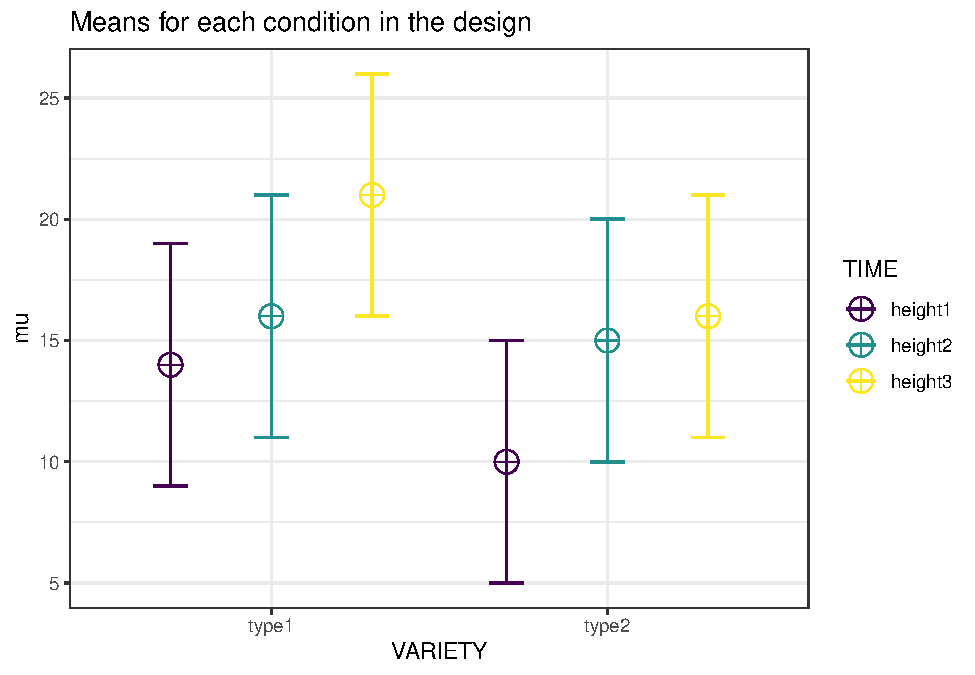
\includegraphics{SuperpowerValidation_files/figure-latex/unnamed-chunk-140-1.pdf}

\begin{Shaded}
\begin{Highlighting}[]
\NormalTok{design\_result}\SpecialCharTok{$}\NormalTok{cor\_mat}
\end{Highlighting}
\end{Shaded}

\begin{verbatim}
##       a1_b1 a1_b2 a1_b3 a2_b1 a2_b2 a2_b3 a3_b1 a3_b2 a3_b3
## a1_b1   1.0   0.8   0.8   0.4   0.4   0.4   0.4   0.4   0.4
## a1_b2   0.8   1.0   0.8   0.4   0.4   0.4   0.4   0.4   0.4
## a1_b3   0.8   0.8   1.0   0.4   0.4   0.4   0.4   0.4   0.4
## a2_b1   0.4   0.4   0.4   1.0   0.8   0.8   0.4   0.4   0.4
## a2_b2   0.4   0.4   0.4   0.8   1.0   0.8   0.4   0.4   0.4
## a2_b3   0.4   0.4   0.4   0.8   0.8   1.0   0.4   0.4   0.4
## a3_b1   0.4   0.4   0.4   0.4   0.4   0.4   1.0   0.8   0.8
## a3_b2   0.4   0.4   0.4   0.4   0.4   0.4   0.8   1.0   0.8
## a3_b3   0.4   0.4   0.4   0.4   0.4   0.4   0.8   0.8   1.0
\end{verbatim}

The design now matches the correlation matrix in Figure 1 of \citet{potvin2000statistical}.

And we can estimate power with \texttt{ANOVA\_exact}.

\begin{Shaded}
\begin{Highlighting}[]
\NormalTok{exact\_result }\OtherTok{\textless{}{-}} \FunctionTok{ANOVA\_exact}\NormalTok{(design\_result,}
                            \AttributeTok{alpha\_level =}\NormalTok{ alpha\_level,}
                            \AttributeTok{verbose =} \ConstantTok{FALSE}\NormalTok{)}
\end{Highlighting}
\end{Shaded}

\begin{table}[!h]

\caption{\label{tab:unnamed-chunk-142}Exact ANOVA Result}
\centering
\begin{tabular}[t]{l|r|r|r|r}
\hline
  & power & partial\_eta\_squared & cohen\_f & non\_centrality\\
\hline
a & 9.441726 & 0.0156250 & 0.1259882 & 0.6031746\\
\hline
b & 100.000000 & 0.7020906 & 1.5351629 & 89.5555556\\
\hline
a:b & 90.092634 & 0.1778846 & 0.4651605 & 16.4444444\\
\hline
\end{tabular}
\end{table}

Further, as we use the analytical solution below, the variance components should be equal to the corresponding MSE from the \texttt{ANOVA\_exact} produced \texttt{anova\_table} object.

\begin{Shaded}
\begin{Highlighting}[]
\NormalTok{exact\_result}\SpecialCharTok{$}\NormalTok{aov\_result}\SpecialCharTok{$}\NormalTok{anova\_table}
\end{Highlighting}
\end{Shaded}

\begin{verbatim}
## Anova Table (Type 3 tests)
## 
## Response: y
##     num Df den Df MSE       F     pes          Pr(>F)    
## a        2     38  35  0.3016 0.01562        0.741397    
## b        2     38   5 44.7778 0.70209 0.0000000001018 ***
## a:b      4     76   5  4.1111 0.17788        0.004542 ** 
## ---
## Signif. codes:  0 '***' 0.001 '**' 0.01 '*' 0.05 '.' 0.1 ' ' 1
\end{verbatim}

\begin{Shaded}
\begin{Highlighting}[]
\NormalTok{k }\OtherTok{\textless{}{-}} \DecValTok{1} \CommentTok{\#one group (because all factors are within)}

\NormalTok{rho\_A }\OtherTok{\textless{}{-}}\NormalTok{ .}\DecValTok{4} \CommentTok{\#mean r for factor A}

\NormalTok{rho\_B }\OtherTok{\textless{}{-}}\NormalTok{ .}\DecValTok{8} \CommentTok{\#mean r for factor B}

\NormalTok{rho\_AB }\OtherTok{\textless{}{-}}\NormalTok{ .}\DecValTok{4} \CommentTok{\#mean r for factor AB}

\NormalTok{alpha }\OtherTok{\textless{}{-}} \FloatTok{0.05}

\NormalTok{sigma }\OtherTok{\textless{}{-}}\NormalTok{ sd}

\NormalTok{m\_A }\OtherTok{\textless{}{-}} \DecValTok{3} \CommentTok{\#levels factor A}

\NormalTok{variance\_e\_A }\OtherTok{\textless{}{-}}\NormalTok{ sigma}\SpecialCharTok{\^{}}\DecValTok{2} \SpecialCharTok{*}\NormalTok{ (}\DecValTok{1} \SpecialCharTok{{-}}\NormalTok{ rho\_A) }\SpecialCharTok{+} 
\NormalTok{  sigma}\SpecialCharTok{\^{}}\DecValTok{2} \SpecialCharTok{*}\NormalTok{ (m\_A }\SpecialCharTok{{-}} \DecValTok{1}\NormalTok{) }\SpecialCharTok{*}\NormalTok{ (rho\_B }\SpecialCharTok{{-}}\NormalTok{ rho\_AB) }
\CommentTok{\#Variance A}
\NormalTok{variance\_e\_A}
\end{Highlighting}
\end{Shaded}

\begin{verbatim}
## [1] 35
\end{verbatim}

\begin{Shaded}
\begin{Highlighting}[]
\NormalTok{m\_B }\OtherTok{\textless{}{-}} \DecValTok{3} \CommentTok{\#levels factor B}

\NormalTok{variance\_e\_B }\OtherTok{\textless{}{-}}\NormalTok{ sigma}\SpecialCharTok{\^{}}\DecValTok{2} \SpecialCharTok{*}\NormalTok{ (}\DecValTok{1} \SpecialCharTok{{-}}\NormalTok{ rho\_B) }\SpecialCharTok{+} 
\NormalTok{  sigma}\SpecialCharTok{\^{}}\DecValTok{2} \SpecialCharTok{*}\NormalTok{ (m\_B }\SpecialCharTok{{-}} \DecValTok{1}\NormalTok{) }\SpecialCharTok{*}\NormalTok{ (rho\_A }\SpecialCharTok{{-}}\NormalTok{ rho\_AB)}
\CommentTok{\#Variance B}
\NormalTok{variance\_e\_B}
\end{Highlighting}
\end{Shaded}

\begin{verbatim}
## [1] 5
\end{verbatim}

\begin{Shaded}
\begin{Highlighting}[]
\NormalTok{variance\_e\_AB }\OtherTok{\textless{}{-}}
\NormalTok{  (sigma }\SpecialCharTok{\^{}} \DecValTok{2} \SpecialCharTok{*}\NormalTok{ (}\DecValTok{1} \SpecialCharTok{{-}} \FunctionTok{max}\NormalTok{(rho\_A, rho\_B)) }\SpecialCharTok{{-}} 
\NormalTok{     sigma }\SpecialCharTok{\^{}} \DecValTok{2} \SpecialCharTok{*}\NormalTok{ (}\FunctionTok{min}\NormalTok{(rho\_A,rho\_B) }\SpecialCharTok{{-}}\NormalTok{ rho\_AB)) }
\CommentTok{\#Variance AB}
\NormalTok{variance\_e\_AB}
\end{Highlighting}
\end{Shaded}

\begin{verbatim}
## [1] 5
\end{verbatim}

\begin{Shaded}
\begin{Highlighting}[]
\CommentTok{\#Create a mean matrix}
\NormalTok{mean\_mat }\OtherTok{\textless{}{-}} \FunctionTok{t}\NormalTok{(}\FunctionTok{matrix}\NormalTok{(mu, }\AttributeTok{nrow =}\NormalTok{ m\_B,}\AttributeTok{ncol =}\NormalTok{ m\_A)) }
\NormalTok{mean\_mat}
\end{Highlighting}
\end{Shaded}

\begin{verbatim}
##      [,1] [,2] [,3]
## [1,]    2  1.0    4
## [2,]    2  0.5    3
## [3,]    2  0.0    6
\end{verbatim}

\begin{Shaded}
\begin{Highlighting}[]
\CommentTok{\# Potvin \& Schutz, 2000, formula 2, p. 348}
\CommentTok{\# For main effect A}
\NormalTok{lambda\_A }\OtherTok{\textless{}{-}}
\NormalTok{  (n }\SpecialCharTok{*}\NormalTok{ m\_A }\SpecialCharTok{*} \FunctionTok{sum}\NormalTok{((}\FunctionTok{rowMeans}\NormalTok{(mean\_mat) }\SpecialCharTok{{-}} 
                   \FunctionTok{mean}\NormalTok{(}\FunctionTok{rowMeans}\NormalTok{(mean\_mat))) }\SpecialCharTok{\^{}} \DecValTok{2}\NormalTok{) ) }\SpecialCharTok{/}\NormalTok{ variance\_e\_A}
\NormalTok{  lambda\_A}
\end{Highlighting}
\end{Shaded}

\begin{verbatim}
## [1] 0.6031746
\end{verbatim}

\begin{Shaded}
\begin{Highlighting}[]
\CommentTok{\#calculate degrees of freedom 1 {-} ignoring the sphericity correction}
\NormalTok{df1 }\OtherTok{\textless{}{-}}\NormalTok{ (m\_A }\SpecialCharTok{{-}} \DecValTok{1}\NormalTok{) }

\NormalTok{df2 }\OtherTok{\textless{}{-}}\NormalTok{ (n }\SpecialCharTok{{-}}\NormalTok{ k) }\SpecialCharTok{*}\NormalTok{ (m\_A }\SpecialCharTok{{-}} \DecValTok{1}\NormalTok{) }\CommentTok{\#calculate degrees of freedom 2}

\NormalTok{F\_critical }\OtherTok{\textless{}{-}} \FunctionTok{qf}\NormalTok{(alpha, }\CommentTok{\# critical F{-}vaue}
\NormalTok{                 df1,}
\NormalTok{                 df2, }
                 \AttributeTok{lower.tail =} \ConstantTok{FALSE}\NormalTok{) }

\NormalTok{pow\_A }\OtherTok{\textless{}{-}} \FunctionTok{pf}\NormalTok{(}\FunctionTok{qf}\NormalTok{(alpha, }\CommentTok{\#power }
\NormalTok{             df1, }
\NormalTok{             df2, }
             \AttributeTok{lower.tail =} \ConstantTok{FALSE}\NormalTok{), }
\NormalTok{          df1, }
\NormalTok{          df2, }
\NormalTok{          lambda\_A, }
          \AttributeTok{lower.tail =} \ConstantTok{FALSE}\NormalTok{)}
\NormalTok{pow\_A}\SpecialCharTok{*}\DecValTok{100}
\end{Highlighting}
\end{Shaded}

\begin{verbatim}
## [1] 9.441726
\end{verbatim}

\begin{Shaded}
\begin{Highlighting}[]
\NormalTok{lambda\_B }\OtherTok{\textless{}{-}}
\NormalTok{  n }\SpecialCharTok{*}\NormalTok{ m\_B }\SpecialCharTok{*} \FunctionTok{sum}\NormalTok{((}\FunctionTok{colMeans}\NormalTok{(mean\_mat) }\SpecialCharTok{{-}} 
                   \FunctionTok{mean}\NormalTok{(}\FunctionTok{colMeans}\NormalTok{(mean\_mat))) }\SpecialCharTok{\^{}} \DecValTok{2}\NormalTok{) }\SpecialCharTok{/}\NormalTok{ variance\_e\_B }
\NormalTok{lambda\_B}
\end{Highlighting}
\end{Shaded}

\begin{verbatim}
## [1] 89.55556
\end{verbatim}

\begin{Shaded}
\begin{Highlighting}[]
\NormalTok{df1 }\OtherTok{\textless{}{-}}\NormalTok{ (m\_B }\SpecialCharTok{{-}} \DecValTok{1}\NormalTok{) }\CommentTok{\#calculate degrees of freedom 1}

\NormalTok{df2 }\OtherTok{\textless{}{-}}\NormalTok{ (n }\SpecialCharTok{{-}}\NormalTok{ k) }\SpecialCharTok{*}\NormalTok{ (m\_B }\SpecialCharTok{{-}} \DecValTok{1}\NormalTok{) }\CommentTok{\#calculate degrees of freedom 2}

\NormalTok{F\_critical }\OtherTok{\textless{}{-}} \FunctionTok{qf}\NormalTok{(alpha, }\CommentTok{\# critical F{-}vaue}
\NormalTok{                 df1,}
\NormalTok{                 df2,}
                 \AttributeTok{lower.tail =} \ConstantTok{FALSE}\NormalTok{) }

\NormalTok{pow\_B }\OtherTok{\textless{}{-}} \FunctionTok{pf}\NormalTok{(}\FunctionTok{qf}\NormalTok{(alpha, }\CommentTok{\#power }
\NormalTok{             df1, }
\NormalTok{             df2, }
             \AttributeTok{lower.tail =} \ConstantTok{FALSE}\NormalTok{), }
\NormalTok{          df1, }
\NormalTok{          df2, }
\NormalTok{          lambda\_B, }
          \AttributeTok{lower.tail =} \ConstantTok{FALSE}\NormalTok{)}


\NormalTok{pow\_B}\SpecialCharTok{*}\DecValTok{100}
\end{Highlighting}
\end{Shaded}

\begin{verbatim}
## [1] 100
\end{verbatim}

\begin{Shaded}
\begin{Highlighting}[]
\CommentTok{\#Peform double summation courtesy of Andrew Vigotsky}
\NormalTok{term }\OtherTok{\textless{}{-}} \DecValTok{0}
\ControlFlowTok{for}\NormalTok{ (i }\ControlFlowTok{in} \DecValTok{1}\SpecialCharTok{:}\FunctionTok{nrow}\NormalTok{(mean\_mat)) \{}
  \ControlFlowTok{for}\NormalTok{ (j }\ControlFlowTok{in} \DecValTok{1}\SpecialCharTok{:}\FunctionTok{ncol}\NormalTok{(mean\_mat)) \{}
\NormalTok{    term }\OtherTok{\textless{}{-}}\NormalTok{ ((term }\SpecialCharTok{+}\NormalTok{ (mean\_mat[i,j] }\SpecialCharTok{{-}}
                        \FunctionTok{mean}\NormalTok{(mean\_mat[i,]) }\SpecialCharTok{{-}} 
                        \FunctionTok{mean}\NormalTok{(mean\_mat[,j]) }\SpecialCharTok{+} \FunctionTok{mean}\NormalTok{(mean\_mat))}\SpecialCharTok{\^{}}\DecValTok{2}\NormalTok{))}
\NormalTok{  \}}
\NormalTok{\}}
\NormalTok{term}
\end{Highlighting}
\end{Shaded}

\begin{verbatim}
## [1] 4.111111
\end{verbatim}

\begin{Shaded}
\begin{Highlighting}[]
\CommentTok{\#Calculate lambda for interaction term}
\NormalTok{lambda\_AB }\OtherTok{\textless{}{-}}\NormalTok{ n}\SpecialCharTok{*}\NormalTok{term}\SpecialCharTok{/}\NormalTok{variance\_e\_AB}
\NormalTok{lambda\_AB}
\end{Highlighting}
\end{Shaded}

\begin{verbatim}
## [1] 16.44444
\end{verbatim}

\begin{Shaded}
\begin{Highlighting}[]
\NormalTok{df1 }\OtherTok{\textless{}{-}}\NormalTok{ (m\_A }\SpecialCharTok{{-}} \DecValTok{1}\NormalTok{) }\SpecialCharTok{*}\NormalTok{ (m\_B }\SpecialCharTok{{-}} \DecValTok{1}\NormalTok{)  }\CommentTok{\#calculate degrees of freedom 1}
\NormalTok{df2 }\OtherTok{\textless{}{-}}
\NormalTok{(n }\SpecialCharTok{{-}}\NormalTok{ k) }\SpecialCharTok{*}\NormalTok{ (m\_A }\SpecialCharTok{{-}} \DecValTok{1}\NormalTok{) }\SpecialCharTok{*}\NormalTok{ (m\_B }\SpecialCharTok{{-}} \DecValTok{1}\NormalTok{) }\CommentTok{\#calculate degrees of freedom 2}
\NormalTok{F\_critical }\OtherTok{\textless{}{-}} \FunctionTok{qf}\NormalTok{(alpha, }\CommentTok{\# critical F{-}vaue}
\NormalTok{df1,}
\NormalTok{df2,}
\AttributeTok{lower.tail =} \ConstantTok{FALSE}\NormalTok{)}

\NormalTok{pow\_AB }\OtherTok{\textless{}{-}} \FunctionTok{pf}\NormalTok{(}\FunctionTok{qf}\NormalTok{(alpha, }\CommentTok{\#power}
\NormalTok{df1,}
\NormalTok{df2,}
\AttributeTok{lower.tail =} \ConstantTok{FALSE}\NormalTok{),}
\NormalTok{df1,}
\NormalTok{df2,}
\NormalTok{lambda\_AB,}
\AttributeTok{lower.tail =} \ConstantTok{FALSE}\NormalTok{)}

\NormalTok{pow\_AB}\SpecialCharTok{*}\DecValTok{100}
\end{Highlighting}
\end{Shaded}

\begin{verbatim}
## [1] 90.09263
\end{verbatim}

Again, when we compile all the analytical results into a single table we can see that the results match those from \texttt{ANOVA\_exact}.

\begin{table}[!h]

\caption{\label{tab:unnamed-chunk-146}Analytical Result}
\centering
\begin{tabular}[t]{r|r|r}
\hline
variance & lambda & power\\
\hline
35 & 0.6031746 & 9.441726\\
\hline
5 & 89.5555556 & 100.000000\\
\hline
5 & 16.4444444 & 90.092634\\
\hline
\end{tabular}
\end{table}

\hypertarget{multivariate-anova-manova}{%
\section{Multivariate ANOVA (MANOVA)}\label{multivariate-anova-manova}}

A large proportion of research with within-subjects manipulations, or repeated measures, rely upon the ``univariate'' approach \citep{maxwell_designing_2004}. While this approach is valid, when corrections for sphercity are applied, it may not be the most powerful or informative analysis plan. Instead, researchers should consider a multivariate analysis (MANOVA). While the MANOVA is not ``assumption free'' it does not assume sphercity which makes it a very attractive analytical tool and the preferred method of analysis for some situations \citep{maxwell_designing_2004}.

For a simple one-way repeated measures design, there are some simple guidelines for power analysis set forth by \citet{maxwell_designing_2004} (pg. 750). All that is needed in the effect size calculated as:
\[ d = \frac{\mu_{max}-\mu_{min}}{\sigma} \]
This assumes that each level has a common standard deviation (i.e., there is only 1 \texttt{sd} input for the design).

In addition, the non-centrality parameter of the \emph{F}-statistic can be estimated from \citet{vonesh1986sample} equations as the following:
\[ \delta^2 = \frac{n \cdot d^2}{2\cdot(1-\rho_{min} )} \]
\newpage
Let us assume we have a \texttt{2w} design with \texttt{mu\ =\ c(0,0.5)}, a common standard deviation of 1 (\texttt{sd=1}), and correlation between \texttt{a1} and \texttt{a2} of r = .4 and a total sample size of 15 (\texttt{n\ =\ 15}) participants.
Power could then be calculated with the following \texttt{R} code.

\begin{Shaded}
\begin{Highlighting}[]
\NormalTok{mu }\OtherTok{=} \FunctionTok{c}\NormalTok{(}\DecValTok{0}\NormalTok{,}\FloatTok{0.5}\NormalTok{)}
\NormalTok{rho }\OtherTok{=}\NormalTok{ .}\DecValTok{4}
\NormalTok{sd }\OtherTok{=} \DecValTok{2}
\NormalTok{n }\OtherTok{=} \DecValTok{15}
\NormalTok{d }\OtherTok{=}\NormalTok{ (}\FunctionTok{max}\NormalTok{(mu)}\SpecialCharTok{{-}}\FunctionTok{min}\NormalTok{(mu))}\SpecialCharTok{/}\NormalTok{sd}
\NormalTok{noncentrality }\OtherTok{=}\NormalTok{ ((n}\SpecialCharTok{*}\NormalTok{d}\SpecialCharTok{\^{}}\DecValTok{2}\NormalTok{) }\SpecialCharTok{/}\NormalTok{ (}\DecValTok{2}\SpecialCharTok{*}\NormalTok{(}\DecValTok{1}\SpecialCharTok{{-}}\FunctionTok{min}\NormalTok{(rho))))}
\NormalTok{noncentrality}
\end{Highlighting}
\end{Shaded}

\begin{verbatim}
## [1] 0.78125
\end{verbatim}

\begin{Shaded}
\begin{Highlighting}[]
\CommentTok{\#Critical F}
\NormalTok{Ft }\OtherTok{\textless{}{-}} \FunctionTok{qf}\NormalTok{((}\DecValTok{1} \SpecialCharTok{{-}}\NormalTok{ .}\DecValTok{05}\NormalTok{), }\DecValTok{1}\NormalTok{, }\DecValTok{14}\NormalTok{)}
\NormalTok{Ft}
\end{Highlighting}
\end{Shaded}

\begin{verbatim}
## [1] 4.60011
\end{verbatim}

\begin{Shaded}
\begin{Highlighting}[]
\CommentTok{\#Power}
\NormalTok{power }\OtherTok{\textless{}{-}}\NormalTok{ (}\DecValTok{1} \SpecialCharTok{{-}} \FunctionTok{pf}\NormalTok{(Ft,}
                 \DecValTok{1}\NormalTok{,}
                 \DecValTok{14}\NormalTok{,}
\NormalTok{                 noncentrality)) }\SpecialCharTok{*} \DecValTok{100}
\NormalTok{power}
\end{Highlighting}
\end{Shaded}

\begin{verbatim}
## [1] 13.07682
\end{verbatim}

\newpage

Now we replicate in \texttt{Superpower}.

\begin{Shaded}
\begin{Highlighting}[]
\NormalTok{design\_result }\OtherTok{\textless{}{-}} \FunctionTok{ANOVA\_design}\NormalTok{(}\StringTok{"2w"}\NormalTok{,}
                              \AttributeTok{n =}\NormalTok{ n,}
                              \AttributeTok{r =}\NormalTok{ rho,}
                              \AttributeTok{sd =}\NormalTok{ sd,}
                              \AttributeTok{mu =}\NormalTok{ mu)}
\end{Highlighting}
\end{Shaded}

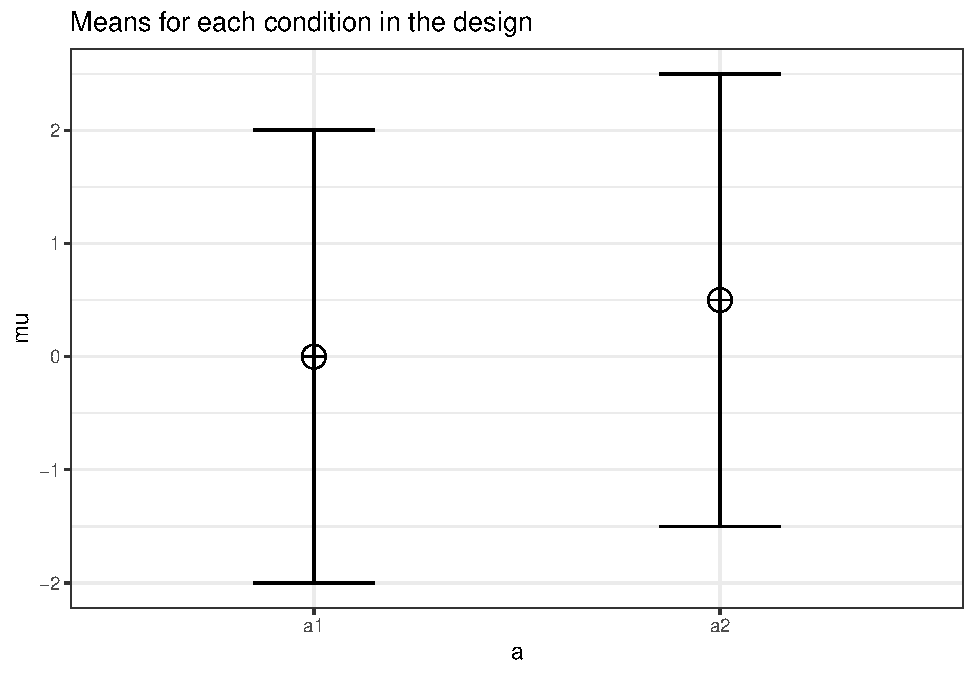
\includegraphics{SuperpowerValidation_files/figure-latex/unnamed-chunk-149-1.pdf}

\begin{Shaded}
\begin{Highlighting}[]
\NormalTok{exact\_result }\OtherTok{\textless{}{-}} \FunctionTok{ANOVA\_exact}\NormalTok{(design\_result, }\AttributeTok{verbose =} \ConstantTok{FALSE}\NormalTok{)}
\end{Highlighting}
\end{Shaded}

\begin{table}[!h]

\caption{\label{tab:unnamed-chunk-150}MANOVA Result}
\centering
\begin{tabular}[t]{l|r|r|r|r}
\hline
  & power & pillai\_trace & cohen\_f & non\_centrality\\
\hline
(Intercept) & 8.401182 & 0.0233572 & 0.1546474 & 0.3348214\\
\hline
a & 13.076818 & 0.0528541 & 0.2362278 & 0.7812500\\
\hline
\end{tabular}
\end{table}

The problem with this formula for determining power is that it is inexact and makes a number of assumptions (\citet{maxwell_designing_2004}, ppg. 752). In reality, it can only give a lower bound estimate of power for a given design, and the actual power may be much higher. This is problematic because it could lead to inefficient study design (e.g., determining you need 20 participants when adequate power could be achieved with less participants). This will become increasingly important in designs with multiple levels and possible violations of the assumption of sphericity.

\hypertarget{mixed-anova}{%
\chapter{Mixed ANOVA}\label{mixed-anova}}

So far we have discussed the simple one-way ANOVA, various forms of the repeated measures ANOVA (and multivariate alternatives), but we have not yet looked at ``mixed ANOVA'' wherein there are between and within subjects factors. Therefore, in this chapter we will show how a power analysis for these designs is performed in \texttt{Superpower}. Further, we will introduce comparisons to SAS's \texttt{PROC\ GLMPOWER} which is a very powerful tool when designing mixed factorial experiments.

\hypertarget{simple-mixed-designs}{%
\section{Simple Mixed Designs}\label{simple-mixed-designs}}

We can simulate a two-way ANOVA with a specific alpha, sample size and effect size, to achieve a specified statistical power. We will try to reproduce the power analysis in g*power \citep{faul2007g} for an F-test from an ANOVA with a repeated measures, within-between interaction effect. While g*power is a great tool it has limited options for mixed factorial ANOVAs.
\newpage 
Let us setup a simple 2x2 design.
For the 2-way interaction, the result should be a power of 91.25\% with at total sample size of 46. Since we have 2 groups in the between -subjects factor that means the sample size per group is 23 with two measurements per subject (i.e., \texttt{2w}).

\includegraphics{screenshots/gpower_5.png}
\newpage

Now, we can repeat the process in \texttt{Superpower}.

\begin{Shaded}
\begin{Highlighting}[]
\NormalTok{mu }\OtherTok{\textless{}{-}} \FunctionTok{c}\NormalTok{(}\SpecialCharTok{{-}}\FloatTok{0.25}\NormalTok{, }\FloatTok{0.25}\NormalTok{, }\FloatTok{0.25}\NormalTok{,}\SpecialCharTok{{-}}\FloatTok{0.25}\NormalTok{)}
\NormalTok{n }\OtherTok{\textless{}{-}} \DecValTok{23}
\NormalTok{sd }\OtherTok{\textless{}{-}} \DecValTok{1}
\NormalTok{r }\OtherTok{\textless{}{-}} \FloatTok{0.5}
\NormalTok{string }\OtherTok{=} \StringTok{"2w*2b"}
\NormalTok{alpha\_level }\OtherTok{\textless{}{-}} \FloatTok{0.05}
\NormalTok{labelnames }\OtherTok{=} \FunctionTok{c}\NormalTok{(}\StringTok{"age"}\NormalTok{, }\StringTok{"old"}\NormalTok{, }\StringTok{"young"}\NormalTok{, }\StringTok{"color"}\NormalTok{, }\StringTok{"blue"}\NormalTok{, }\StringTok{"red"}\NormalTok{)}
\NormalTok{design\_result }\OtherTok{\textless{}{-}} \FunctionTok{ANOVA\_design}\NormalTok{(}
\AttributeTok{design =}\NormalTok{ string,}
\AttributeTok{n =}\NormalTok{ n,}
\AttributeTok{mu =}\NormalTok{ mu,}
\AttributeTok{sd =}\NormalTok{ sd,}
\AttributeTok{r =}\NormalTok{ r,}
\AttributeTok{labelnames =}\NormalTok{ labelnames}
\NormalTok{)}
\end{Highlighting}
\end{Shaded}

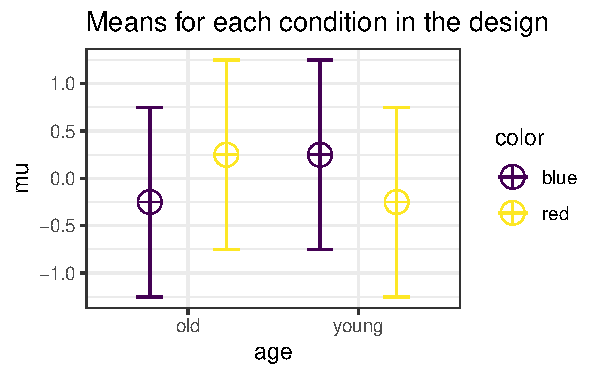
\includegraphics{SuperpowerValidation_files/figure-latex/start_mixedANOVA-1.pdf}

\begin{Shaded}
\begin{Highlighting}[]
\NormalTok{simulation\_result }\OtherTok{\textless{}{-}} \FunctionTok{ANOVA\_power}\NormalTok{(design\_result, }
                                 \AttributeTok{alpha\_level =}\NormalTok{ alpha\_level, }
                                 \AttributeTok{nsims =}\NormalTok{ nsims,}
                                 \AttributeTok{verbose =} \ConstantTok{FALSE}\NormalTok{)}
\end{Highlighting}
\end{Shaded}

\begin{table}[!h]

\caption{\label{tab:unnamed-chunk-152}Simulated ANOVA Result}
\centering
\begin{tabular}[t]{l|r|r}
\hline
  & power & effect\_size\\
\hline
anova\_color & 4.89 & 0.0219823\\
\hline
anova\_age & 5.20 & 0.0225908\\
\hline
anova\_color:age & 91.22 & 0.2151983\\
\hline
\end{tabular}
\end{table}

\begin{Shaded}
\begin{Highlighting}[]
\NormalTok{exact\_result }\OtherTok{\textless{}{-}} \FunctionTok{ANOVA\_exact}\NormalTok{(design\_result,}
                            \AttributeTok{alpha\_level =}\NormalTok{ alpha\_level,}
                            \AttributeTok{verbose =} \ConstantTok{FALSE}\NormalTok{)}
\end{Highlighting}
\end{Shaded}

\begin{table}[!h]

\caption{\label{tab:unnamed-chunk-154}Exact ANOVA Result}
\centering
\begin{tabular}[t]{l|r|r|r|r}
\hline
  & power & partial\_eta\_squared & cohen\_f & non\_centrality\\
\hline
color & 5.00000 & 0.0000000 & 0.0000000 & 0.0\\
\hline
age & 5.00000 & 0.0000000 & 0.0000000 & 0.0\\
\hline
color:age & 91.24984 & 0.2072072 & 0.5112374 & 11.5\\
\hline
\end{tabular}
\end{table}

\newpage

Now, we can simulate the same two-way ANOVA but increasing the correlation to r=0.7.

\includegraphics{screenshots/gpower_6.png}
\newpage

\begin{Shaded}
\begin{Highlighting}[]
\NormalTok{mu }\OtherTok{\textless{}{-}} \FunctionTok{c}\NormalTok{(}\SpecialCharTok{{-}}\FloatTok{0.25}\NormalTok{, }\FloatTok{0.25}\NormalTok{, }\FloatTok{0.25}\NormalTok{, }\SpecialCharTok{{-}}\FloatTok{0.25}\NormalTok{)}
\NormalTok{n }\OtherTok{\textless{}{-}} \DecValTok{23}
\NormalTok{sd }\OtherTok{\textless{}{-}} \DecValTok{1}
\NormalTok{r }\OtherTok{\textless{}{-}} \FloatTok{0.7}
\NormalTok{string }\OtherTok{=} \StringTok{"2w*2b"}
\NormalTok{alpha\_level }\OtherTok{\textless{}{-}} \FloatTok{0.05}
\NormalTok{labelnames }\OtherTok{=} \FunctionTok{c}\NormalTok{(}\StringTok{"age"}\NormalTok{, }\StringTok{"old"}\NormalTok{, }\StringTok{"young"}\NormalTok{, }\StringTok{"color"}\NormalTok{, }\StringTok{"blue"}\NormalTok{, }\StringTok{"red"}\NormalTok{)}
\NormalTok{design\_result }\OtherTok{\textless{}{-}} \FunctionTok{ANOVA\_design}\NormalTok{(}\AttributeTok{design =}\NormalTok{ string,}
                              \AttributeTok{n =}\NormalTok{ n, }
                              \AttributeTok{mu =}\NormalTok{ mu, }
                              \AttributeTok{sd =}\NormalTok{ sd, }
                              \AttributeTok{r =}\NormalTok{ r, }
                              \AttributeTok{labelnames =}\NormalTok{ labelnames)}
\end{Highlighting}
\end{Shaded}

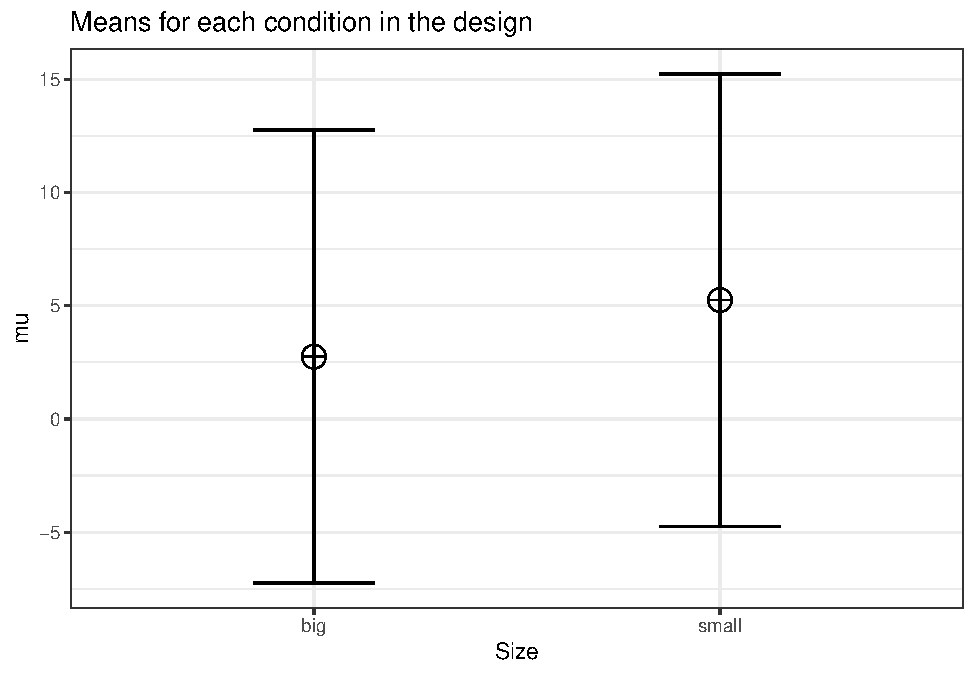
\includegraphics{SuperpowerValidation_files/figure-latex/unnamed-chunk-155-1.pdf}

\begin{Shaded}
\begin{Highlighting}[]
\NormalTok{simulation\_result }\OtherTok{\textless{}{-}} \FunctionTok{ANOVA\_power}\NormalTok{(design\_result, }
                                 \AttributeTok{alpha\_level =}\NormalTok{ alpha\_level, }
                                 \AttributeTok{nsims =}\NormalTok{ nsims,}
                                 \AttributeTok{verbose =} \ConstantTok{FALSE}\NormalTok{)}
\end{Highlighting}
\end{Shaded}

\begin{table}[!h]

\caption{\label{tab:unnamed-chunk-157}Simulated ANOVA Result}
\centering
\begin{tabular}[t]{l|r|r}
\hline
  & power & effect\_size\\
\hline
anova\_color & 5.14 & 0.0220381\\
\hline
anova\_age & 4.78 & 0.0219031\\
\hline
anova\_color:age & 99.03 & 0.3066459\\
\hline
\end{tabular}
\end{table}

\begin{Shaded}
\begin{Highlighting}[]
\NormalTok{exact\_result }\OtherTok{\textless{}{-}} \FunctionTok{ANOVA\_exact}\NormalTok{(design\_result,}
                            \AttributeTok{alpha\_level =}\NormalTok{ alpha\_level,}
                            \AttributeTok{verbose =} \ConstantTok{FALSE}\NormalTok{)}
\end{Highlighting}
\end{Shaded}

\begin{table}[!h]

\caption{\label{tab:unnamed-chunk-159}Exact ANOVA Result}
\centering
\begin{tabular}[t]{l|r|r|r|r}
\hline
  & power & partial\_eta\_squared & cohen\_f & non\_centrality\\
\hline
color & 5.00000 & 0.0000000 & 0.0000000 & 0.00000\\
\hline
age & 5.00000 & 0.0000000 & 0.0000000 & 0.00000\\
\hline
color:age & 98.98467 & 0.3034301 & 0.6600046 & 19.16667\\
\hline
\end{tabular}
\end{table}

\newpage

\hypertarget{complex-mixed-designs}{%
\section{Complex Mixed Designs}\label{complex-mixed-designs}}

Now, we are to the most complicated calculations. Similiar to the simple one-way repeated measures ANOVA, a mixed ANOVA assumes sphercity. Therefore, in most situations a multivariate approach, MANOVA, is recommended \citep{maxwell_designing_2004}. To our knowledge, the only program that can accurately calculate power for mixed designs with greater than 2 levels is SAS's \texttt{PROC\ GLMPOWER} \citep{SASglmpower}. The procedure utilizes approximate analytical solutions derived by \citet{muller1984practical} and \citet{o1999pragmatic}. According to the documentation, these analytical solutions are very accurate for all but small N situations (sorry exercise scientists!). Eventually, this chapter will document the analytical solution in a step-by-step fashion, but for the time being we will just directly compare \texttt{Superpower} to \texttt{GLMPOWER} from a few examples provided by SAS.

\hypertarget{b3w-design}{%
\subsection{2b*3w Design}\label{b3w-design}}

Here we will use a modified example from \citet{SASglmpower} pg. 3739. In this hypothetical experiment, suppose you are planning an experiment to study the growth of two varieties of flowers over the course of 3 weeks. The planned data analysis is a two-way ANOVA with flower height as the outcome and a model with effects of time, flower variety, and their interaction.

First we can set up the dataframe in SAS. This is similiar to the \texttt{mu} command in \texttt{ANOVA\_design}.

\begin{Shaded}
\begin{Highlighting}[]
\NormalTok{data Exemplary2;}
\NormalTok{input variety Height1 Height2 Height3;}
\NormalTok{datalines;}
\DecValTok{1} \DecValTok{14} \DecValTok{16} \DecValTok{21}
\DecValTok{2} \DecValTok{10} \DecValTok{15} \DecValTok{16}
\NormalTok{;}
\end{Highlighting}
\end{Shaded}

We can now solve for power in \texttt{PROC\ GLMPOWER}. In this case, we set up a multivariate repeated measures model, with a total of 40 flowers (20 per variety). We also setup the within-factor correlations with the CORRS command.

\begin{Shaded}
\begin{Highlighting}[]
\NormalTok{proc glmpower data}\OtherTok{=}\NormalTok{Exemplary2;}
\NormalTok{class Variety Exposure;}
\NormalTok{model Height1 Height2 Height3 }\OtherTok{=}\NormalTok{ Variety;}
\NormalTok{repeated Time contrast;}
\NormalTok{power}
\NormalTok{mtest }\OtherTok{=}\NormalTok{ pt}
\NormalTok{stddev }\OtherTok{=} \DecValTok{5}
\NormalTok{ntotal }\OtherTok{=} \DecValTok{40}
\NormalTok{power }\OtherTok{=}\NormalTok{ .}
\FunctionTok{MATRIX}\NormalTok{(}\StringTok{"MyCorrs"}\NormalTok{)}\OtherTok{=}\NormalTok{ (.}\DecValTok{75}\NormalTok{,}
                    \FloatTok{0.5625}\NormalTok{,.}\DecValTok{75}\NormalTok{)}
\NormalTok{CORRS}\OtherTok{=} \StringTok{"MyCorrs"}\NormalTok{;}
\NormalTok{run;}
\end{Highlighting}
\end{Shaded}

The power analysis results then get printed to the SAS ouput page.

\includegraphics{screenshots/sas_2x3repeated.png}

Now let's replicate this in \texttt{R} with \texttt{Superpower}. First, we setup the same design with \texttt{ANOVA\_design}.

\begin{Shaded}
\begin{Highlighting}[]
\NormalTok{cor\_1 }\OtherTok{\textless{}{-}} \FunctionTok{matrix}\NormalTok{(}\FunctionTok{c}\NormalTok{(}\DecValTok{1}\NormalTok{, .}\DecValTok{75}\NormalTok{, .}\DecValTok{5625}\NormalTok{,}
\NormalTok{                  .}\DecValTok{75}\NormalTok{, }\DecValTok{1}\NormalTok{, .}\DecValTok{75}\NormalTok{,}
\NormalTok{                  .}\DecValTok{5625}\NormalTok{, .}\DecValTok{75}\NormalTok{, }\DecValTok{1}\NormalTok{), }\AttributeTok{nrow=}\DecValTok{3}\NormalTok{)}

\NormalTok{cor\_2 }\OtherTok{\textless{}{-}}\NormalTok{ cor\_1}\SpecialCharTok{*}\DecValTok{0}

\NormalTok{rho\_mat }\OtherTok{\textless{}{-}} \FunctionTok{cbind}\NormalTok{(}\FunctionTok{rbind}\NormalTok{(cor\_1,cor\_2),}
                      \FunctionTok{rbind}\NormalTok{(cor\_2,cor\_1))}

\NormalTok{design\_result }\OtherTok{\textless{}{-}} \FunctionTok{ANOVA\_design}\NormalTok{(}\StringTok{"2b*3w"}\NormalTok{,}
                              \AttributeTok{n =} \DecValTok{20}\NormalTok{,}
                              \AttributeTok{sd =} \DecValTok{5}\NormalTok{,}
                              \AttributeTok{mu =} \FunctionTok{c}\NormalTok{(}\DecValTok{14}\NormalTok{, }\DecValTok{16}\NormalTok{, }\DecValTok{21}\NormalTok{,}
                                     \DecValTok{10}\NormalTok{, }\DecValTok{15}\NormalTok{, }\DecValTok{16}\NormalTok{),}
                              \AttributeTok{r =}\NormalTok{ rho\_mat,}
                              \AttributeTok{labelnames =} \FunctionTok{c}\NormalTok{(}\StringTok{"VARIETY"}\NormalTok{, }
                                             \StringTok{"type1"}\NormalTok{, }\StringTok{"type2"}\NormalTok{,}
                                             \StringTok{"TIME"}\NormalTok{, }
                                             \StringTok{"height1"}\NormalTok{, }\StringTok{"height2"}\NormalTok{, }
                                             \StringTok{"height3"}\NormalTok{),}
                              \AttributeTok{plot =} \ConstantTok{TRUE}\NormalTok{)}
\end{Highlighting}
\end{Shaded}

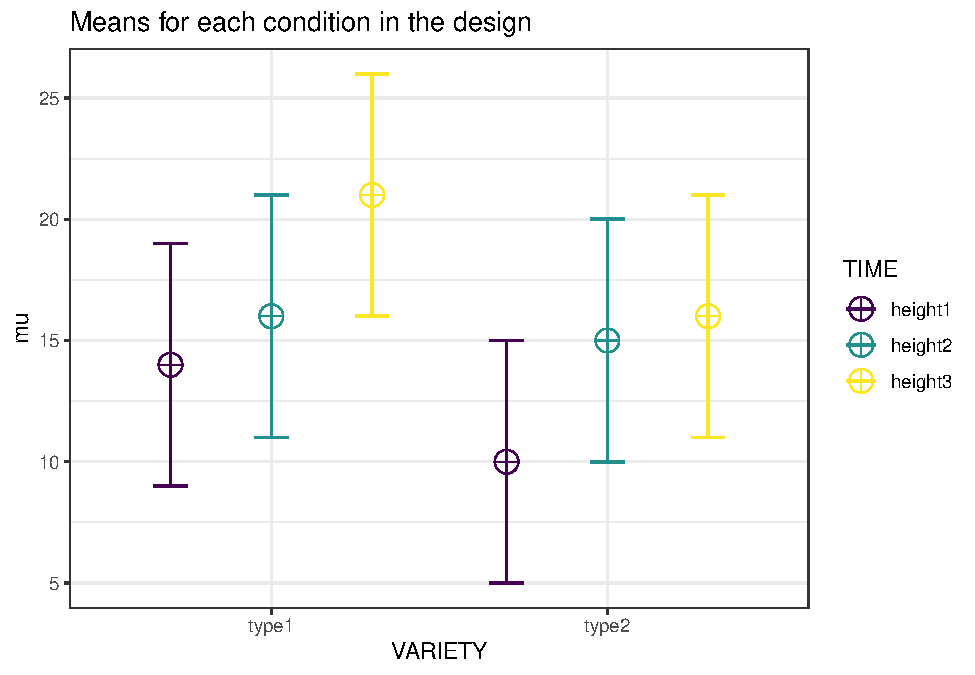
\includegraphics{SuperpowerValidation_files/figure-latex/unnamed-chunk-162-1.pdf}

\begin{Shaded}
\begin{Highlighting}[]
\NormalTok{exact\_result }\OtherTok{\textless{}{-}} \FunctionTok{ANOVA\_exact}\NormalTok{(design\_result, }\AttributeTok{verbose =} \ConstantTok{FALSE}\NormalTok{,}
                            \AttributeTok{correction =} \StringTok{"none"}\NormalTok{,}
                            \AttributeTok{alpha\_level =}\NormalTok{ .}\DecValTok{05}\NormalTok{)}
\end{Highlighting}
\end{Shaded}

\begin{table}[!h]

\caption{\label{tab:unnamed-chunk-164}MANOVA Result}
\centering
\begin{tabular}[t]{l|r|r|r|r}
\hline
  & power & partial\_eta\_squared & cohen\_f & non\_centrality\\
\hline
VARIETY & 63.65566 & 0.1287208 & 0.3843667 & 5.614035\\
\hline
TIME & 100.00000 & 0.5877929 & 1.1941377 & 108.373333\\
\hline
VARIETY:TIME & 84.08029 & 0.1273729 & 0.3820535 & 11.093333\\
\hline
\end{tabular}
\end{table}

You will notice a small discrepancy between the two power estimates for the main effect of variety. This difference is due to the analytical solutions problems with small sample sizes. You will see in the example below that the results match when the total sample size is much greater.

\hypertarget{b4w-design}{%
\subsection{2b*4w Design}\label{b4w-design}}

Now we move onto the example from pg 3794 of \citet{SASglmpower}.

As stated in the manual:

\begin{quote}
Logan, Baron, and Kohout (1995) and Guo et al.~(2013) study the effect of a dental intervention on the
memory of pain after root canal therapy. The intervention is a sensory focus strategy, in which patients are
instructed to pay attention only to the physical sensations in their mouth during the root canal procedure.
Suppose you are interested in the long-term effects of this sensory focus intervention, because avoidance
behavior has been shown to build along with memory of pain. You are planning a study to compare
sensory focus to standard of care over a period of a year, asking patients to self-report their memory of pain
immediately after the procedure and then again at 1 week, 6 months, and 12 months. You use a scale from 0
(no pain remembered) to 5 (maximum pain remembered).
\end{quote}

This makes it a \texttt{2b*4w} design with treatment as a between subjects factor, with two levels (sensory focus versus standard of care), and time as a within-subject factor is time, with four levels (0, 1, 26, and 52 weeks). In this case, we differ from \citet{SASglmpower} and we will solve for power with a sample size of 300 per group (600 total) with an alpha of \texttt{.01}. In addition, we want to see what the impact of chaning the common standard deviation will have on power.

So in SAS we set up the data.

\begin{Shaded}
\begin{Highlighting}[]
\NormalTok{data Pain;}
\NormalTok{input Treatment }\SpecialCharTok{$}\NormalTok{ PainMem0 PainMem1Wk PainMem6Mo PainMem12Mo;}
\NormalTok{datalines;}
\NormalTok{SensoryFocus }\FloatTok{2.40} \FloatTok{2.38} \FloatTok{2.05} \FloatTok{1.90}
\NormalTok{StandardOfCare }\FloatTok{2.40} \FloatTok{2.39} \FloatTok{2.36} \FloatTok{2.30}
\NormalTok{;}
\end{Highlighting}
\end{Shaded}

Then we can run the analysis in SAS. Note that in the example \citet{SASglmpower} are assuming a linear exponential covariance matrix, which we can mimic in \texttt{R}.

\begin{Shaded}
\begin{Highlighting}[]
\NormalTok{proc glmpower data}\OtherTok{=}\NormalTok{Pain;}
\NormalTok{class Treatment;}
\NormalTok{model PainMem0 PainMem1Wk PainMem6Mo PainMem12Mo }\OtherTok{=}\NormalTok{ Treatment;}
\NormalTok{repeated Time contrast;}
\NormalTok{power}
\NormalTok{mtest }\OtherTok{=}\NormalTok{ pt }
\NormalTok{alpha }\OtherTok{=} \FloatTok{0.01}
\NormalTok{power }\OtherTok{=}\NormalTok{ .}
\NormalTok{ntotal }\OtherTok{=} \DecValTok{600}
\NormalTok{stddev }\OtherTok{=} \FloatTok{0.92} \FloatTok{1.04}
\FunctionTok{matrix}\NormalTok{ (}\StringTok{"PainCorr"}\NormalTok{) }\OtherTok{=} \FunctionTok{lear}\NormalTok{(}\FloatTok{0.6}\NormalTok{, }\FloatTok{0.8}\NormalTok{, }\DecValTok{4}\NormalTok{, }\DecValTok{0} \DecValTok{1} \DecValTok{26} \DecValTok{52}\NormalTok{)}
\NormalTok{corrmat }\OtherTok{=} \StringTok{"PainCorr"}\NormalTok{;}
\NormalTok{run;}
\NormalTok{quit;}
\end{Highlighting}
\end{Shaded}

This produces a table with the result for a power analysis with 2 different common standard deviations.

\includegraphics{screenshots/sas_pain.png}

We then replicate in \texttt{R}, first by setting up the ``lear'' correlation matrix.

\begin{Shaded}
\begin{Highlighting}[]
\NormalTok{cor\_1 }\OtherTok{\textless{}{-}} \FunctionTok{matrix}\NormalTok{(}\FunctionTok{c}\NormalTok{(}\DecValTok{1}\NormalTok{,.}\DecValTok{6}\NormalTok{,.}\DecValTok{491}\NormalTok{,.}\DecValTok{399}\NormalTok{,}
\NormalTok{                  .}\DecValTok{6}\NormalTok{,}\DecValTok{1}\NormalTok{,.}\DecValTok{495}\NormalTok{,.}\DecValTok{402}\NormalTok{,}
\NormalTok{                  .}\DecValTok{491}\NormalTok{,.}\DecValTok{495}\NormalTok{,}\DecValTok{1}\NormalTok{,.}\DecValTok{491}\NormalTok{,}
\NormalTok{                  .}\DecValTok{399}\NormalTok{,.}\DecValTok{402}\NormalTok{,.}\DecValTok{491}\NormalTok{,}\DecValTok{1}\NormalTok{), }\AttributeTok{nrow=}\DecValTok{4}\NormalTok{)}

\NormalTok{cor\_2 }\OtherTok{\textless{}{-}}\NormalTok{ cor\_1}\SpecialCharTok{*}\DecValTok{0}

\NormalTok{pain\_cor\_mat }\OtherTok{\textless{}{-}} \FunctionTok{cbind}\NormalTok{(}\FunctionTok{rbind}\NormalTok{(cor\_1,cor\_2),}
                      \FunctionTok{rbind}\NormalTok{(cor\_2,cor\_1))}

\NormalTok{design\_result }\OtherTok{\textless{}{-}} \FunctionTok{ANOVA\_design}\NormalTok{(}\StringTok{"2b*4w"}\NormalTok{,}
                              \AttributeTok{n =} \DecValTok{300}\NormalTok{,}
                              \AttributeTok{mu =} \FunctionTok{c}\NormalTok{(}\FloatTok{2.4}\NormalTok{, }\FloatTok{2.38}\NormalTok{, }\FloatTok{2.05}\NormalTok{, }\FloatTok{1.90}\NormalTok{,}
                                     \FloatTok{2.4}\NormalTok{, }\FloatTok{2.39}\NormalTok{, }\FloatTok{2.36}\NormalTok{, }\FloatTok{2.30}\NormalTok{),}
                              \AttributeTok{sd =}\NormalTok{ .}\DecValTok{92}\NormalTok{,}
                              \AttributeTok{r =}\NormalTok{ pain\_cor\_mat,}
                              \AttributeTok{labelnames =} \FunctionTok{c}\NormalTok{(}\StringTok{"Treatment"}\NormalTok{, }\StringTok{"sensory"}\NormalTok{, }\StringTok{"standard"}\NormalTok{,}
                                             \StringTok{"TIME"}\NormalTok{, }\StringTok{"t1"}\NormalTok{, }\StringTok{"t2"}\NormalTok{, }\StringTok{"t3"}\NormalTok{, }\StringTok{"t4"}\NormalTok{),}
                              \AttributeTok{plot =} \ConstantTok{TRUE}\NormalTok{)}
\end{Highlighting}
\end{Shaded}

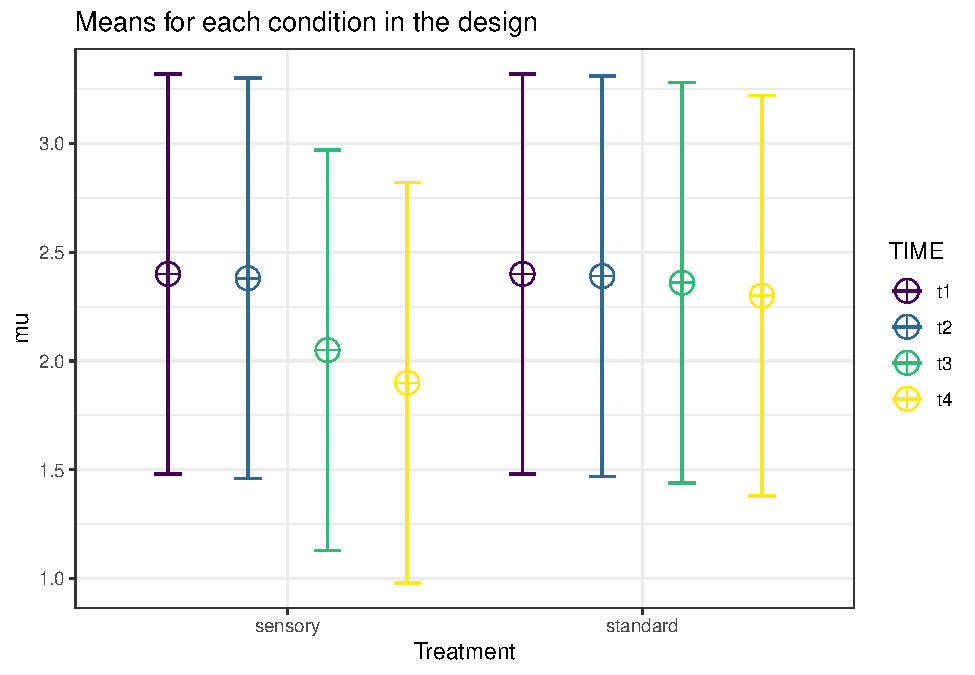
\includegraphics{SuperpowerValidation_files/figure-latex/mixed_multivariate_1-1.pdf}

\begin{Shaded}
\begin{Highlighting}[]
\NormalTok{exact\_result }\OtherTok{\textless{}{-}} \FunctionTok{ANOVA\_exact}\NormalTok{(design\_result, }\AttributeTok{verbose =} \ConstantTok{FALSE}\NormalTok{,}
                            \AttributeTok{alpha\_level =}\NormalTok{ .}\DecValTok{01}\NormalTok{)}
\end{Highlighting}
\end{Shaded}

\begin{table}[!h]

\caption{\label{tab:unnamed-chunk-167}Simulated MANOVA Result}
\centering
\begin{tabular}[t]{l|r|r|r|r}
\hline
  & power & pillai\_trace & cohen\_f & non\_centrality\\
\hline
(Intercept) & 100.00000 & 0.9094197 & 3.1685838 & 6003.874016\\
\hline
Treatment & 68.59334 & 0.0155032 & 0.1254885 & 9.416918\\
\hline
TIME & 99.99995 & 0.0998664 & 0.3330858 & 66.123912\\
\hline
Treatment:TIME & 99.55718 & 0.0531965 & 0.2370344 & 33.486447\\
\hline
\end{tabular}
\end{table}

\begin{Shaded}
\begin{Highlighting}[]
\NormalTok{design\_result }\OtherTok{\textless{}{-}} \FunctionTok{ANOVA\_design}\NormalTok{(}\StringTok{"2b*4w"}\NormalTok{,}
                              \AttributeTok{n =} \DecValTok{300}\NormalTok{,}
                              \AttributeTok{mu =} \FunctionTok{c}\NormalTok{(}\FloatTok{2.4}\NormalTok{, }\FloatTok{2.38}\NormalTok{, }\FloatTok{2.05}\NormalTok{, }\FloatTok{1.90}\NormalTok{,}
                                     \FloatTok{2.4}\NormalTok{, }\FloatTok{2.39}\NormalTok{, }\FloatTok{2.36}\NormalTok{, }\FloatTok{2.30}\NormalTok{),}
                              \AttributeTok{sd =} \FloatTok{1.04}\NormalTok{,}
                              \AttributeTok{r =}\NormalTok{ pain\_cor\_mat,}
                              \AttributeTok{labelnames =} \FunctionTok{c}\NormalTok{(}\StringTok{"Treatment"}\NormalTok{, }\StringTok{"sensory"}\NormalTok{, }\StringTok{"standard"}\NormalTok{,}
                                             \StringTok{"TIME"}\NormalTok{, }\StringTok{"t1"}\NormalTok{, }\StringTok{"t2"}\NormalTok{, }\StringTok{"t3"}\NormalTok{, }\StringTok{"t4"}\NormalTok{),}
                              \AttributeTok{plot =} \ConstantTok{TRUE}\NormalTok{)}
\end{Highlighting}
\end{Shaded}

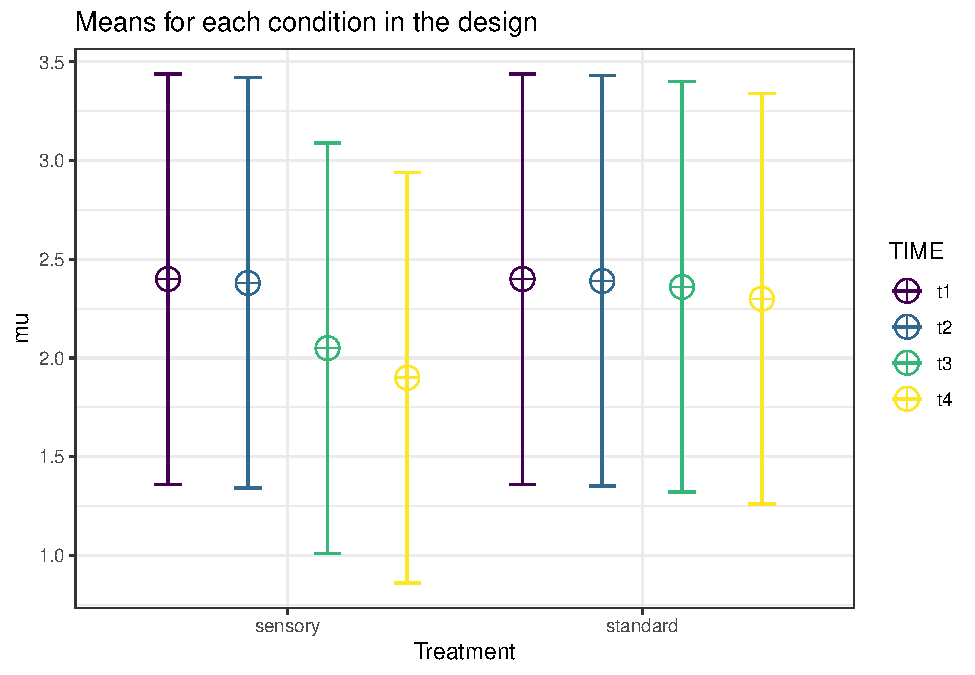
\includegraphics{SuperpowerValidation_files/figure-latex/unnamed-chunk-168-1.pdf}

\begin{Shaded}
\begin{Highlighting}[]
\NormalTok{exact\_result }\OtherTok{\textless{}{-}} \FunctionTok{ANOVA\_exact}\NormalTok{(design\_result, }\AttributeTok{verbose =} \ConstantTok{FALSE}\NormalTok{,}
                            \AttributeTok{alpha\_level =}\NormalTok{ .}\DecValTok{01}\NormalTok{)}
\end{Highlighting}
\end{Shaded}

\begin{table}[!h]

\caption{\label{tab:unnamed-chunk-169}Simulated MANOVA Result}
\centering
\begin{tabular}[t]{l|r|r|r|r}
\hline
  & power & pillai\_trace & cohen\_f & non\_centrality\\
\hline
(Intercept) & 100.00000 & 0.8870909 & 2.8029779 & 4698.297861\\
\hline
Treatment & 55.22151 & 0.0121730 & 0.1110090 & 7.369156\\
\hline
TIME & 99.99672 & 0.0798847 & 0.2946528 & 51.744895\\
\hline
Treatment:TIME & 97.55110 & 0.0421158 & 0.2096843 & 26.204631\\
\hline
\end{tabular}
\end{table}

As we can see, the results for this analysis match SAS perfectly.

\hypertarget{power-for-three-way-interactions}{%
\chapter{Power for Three-way Interactions}\label{power-for-three-way-interactions}}

There are almost no software solutions that allow researchers to perform power anaysis for more complex designs. Through simulation, it is relatively straightforward to examine the power for designs with multiple factors with many levels.

Let's start with a 2x2x2 between-subjects design. We collect 50 participants in each between participant condition (so 400 participants in total - \(50(n)\times2(levels)\times2(levels)\times2(levels)= 400\)).

\begin{Shaded}
\begin{Highlighting}[]
\CommentTok{\# With 2x2x2 designs, }
\CommentTok{\# the names for paired comparisons can become very long. }
\CommentTok{\# So here I abbreviate terms: }
\CommentTok{\#   Size, Color, and Cognitive Load, have values:}
\CommentTok{\# b = big, s = small, g = green, }
\CommentTok{\# r = red, pres = present, abs = absent.  }
\NormalTok{labelnames }\OtherTok{\textless{}{-}} \FunctionTok{c}\NormalTok{(}\StringTok{"Size"}\NormalTok{, }\StringTok{"b"}\NormalTok{, }\StringTok{"s"}\NormalTok{, }\StringTok{"Color"}\NormalTok{, }\StringTok{"g"}\NormalTok{, }\StringTok{"r"}\NormalTok{, }
                \StringTok{"Load"}\NormalTok{, }\StringTok{"pres"}\NormalTok{, }\StringTok{"abs"}\NormalTok{) }\CommentTok{\#}
\NormalTok{design\_result }\OtherTok{\textless{}{-}} \FunctionTok{ANOVA\_design}\NormalTok{(}\AttributeTok{design =} \StringTok{"2b*2b*2b"}\NormalTok{, }
                              \CommentTok{\#sample size per group }
                              \AttributeTok{n =} \DecValTok{50}\NormalTok{, }
                              \CommentTok{\#pattern of means}
                              \AttributeTok{mu =} \FunctionTok{c}\NormalTok{(}\DecValTok{2}\NormalTok{, }\DecValTok{2}\NormalTok{, }\DecValTok{6}\NormalTok{, }\DecValTok{1}\NormalTok{, }\DecValTok{6}\NormalTok{, }\DecValTok{6}\NormalTok{, }\DecValTok{1}\NormalTok{, }\DecValTok{8}\NormalTok{), }
                              \AttributeTok{sd =} \DecValTok{10}\NormalTok{, }\CommentTok{\#standard deviation}
                              \AttributeTok{labelnames =}\NormalTok{ labelnames) }
\end{Highlighting}
\end{Shaded}

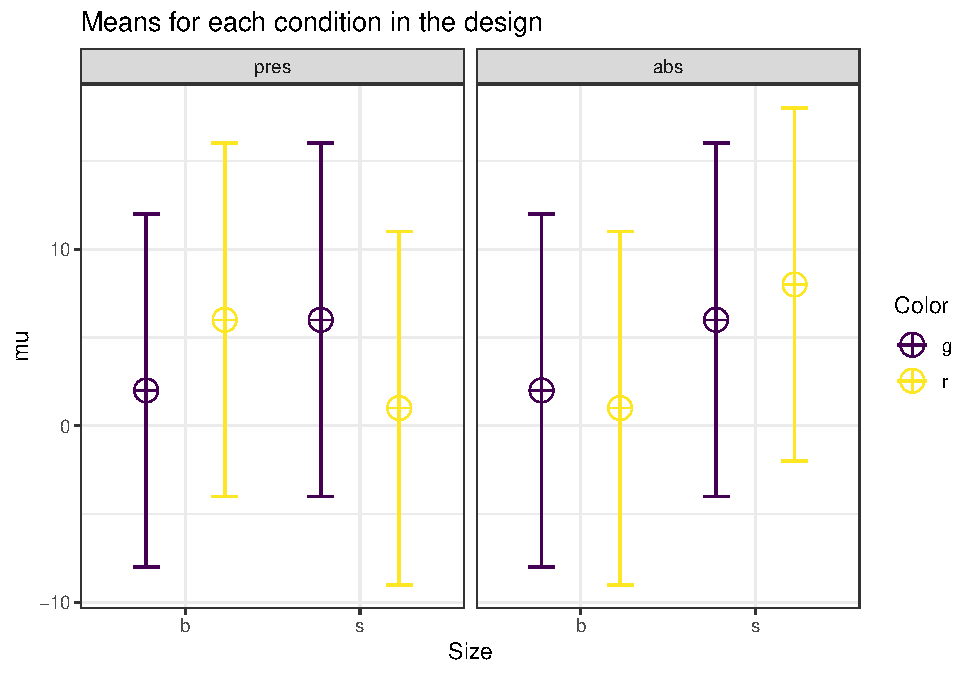
\includegraphics{SuperpowerValidation_files/figure-latex/start_threewayinteraction-1.pdf}

\begin{Shaded}
\begin{Highlighting}[]
\NormalTok{simulation\_result }\OtherTok{\textless{}{-}} \FunctionTok{ANOVA\_power}\NormalTok{(design\_result, }
                                 \AttributeTok{alpha\_level =}\NormalTok{ alpha\_level, }
                                 \AttributeTok{nsims =}\NormalTok{ nsims,}
                                 \AttributeTok{verbose =} \ConstantTok{FALSE}\NormalTok{)}
\end{Highlighting}
\end{Shaded}

\begin{table}[!h]

\caption{\label{tab:unnamed-chunk-172}Simulated ANOVA Result}
\centering
\begin{tabular}[t]{l|r|r}
\hline
  & power & effect\_size\\
\hline
anova\_Size & 70.17 & 0.0179159\\
\hline
anova\_Color & 4.86 & 0.0025370\\
\hline
anova\_Load & 8.31 & 0.0032647\\
\hline
anova\_Size:Color & 31.89 & 0.0081783\\
\hline
anova\_Size:Load & 85.45 & 0.0248185\\
\hline
anova\_Color:Load & 7.80 & 0.0031794\\
\hline
anova\_Size:Color:Load & 85.60 & 0.0248853\\
\hline
\end{tabular}
\end{table}

\begin{Shaded}
\begin{Highlighting}[]
\NormalTok{exact\_result }\OtherTok{\textless{}{-}} \FunctionTok{ANOVA\_exact}\NormalTok{(design\_result,}
                            \AttributeTok{alpha\_level =}\NormalTok{ alpha\_level,}
                            \AttributeTok{verbose =} \ConstantTok{FALSE}\NormalTok{)}
\end{Highlighting}
\end{Shaded}

\begin{table}[!h]

\caption{\label{tab:unnamed-chunk-174}Exact ANOVA Result}
\centering
\begin{tabular}[t]{l|r|r|r|r}
\hline
  & power & partial\_eta\_squared & cohen\_f & non\_centrality\\
\hline
Size & 70.330132 & 0.0156937 & 0.1262691 & 6.25\\
\hline
Color & 5.000000 & 0.0000000 & 0.0000000 & 0.00\\
\hline
Load & 7.895322 & 0.0006373 & 0.0252538 & 0.25\\
\hline
Size:Color & 32.172729 & 0.0057070 & 0.0757614 & 2.25\\
\hline
Size:Load & 84.912313 & 0.0224439 & 0.1515229 & 9.00\\
\hline
Color:Load & 7.895322 & 0.0006373 & 0.0252538 & 0.25\\
\hline
Size:Color:Load & 84.912313 & 0.0224439 & 0.1515229 & 9.00\\
\hline
\end{tabular}
\end{table}

\begin{Shaded}
\begin{Highlighting}[]
\CommentTok{\#Analytical power calculation}
\NormalTok{power\_analytic }\OtherTok{\textless{}{-}} \FunctionTok{power\_threeway\_between}\NormalTok{(design\_result)}
\NormalTok{power\_analytic}\SpecialCharTok{$}\NormalTok{power\_A}
\end{Highlighting}
\end{Shaded}

\begin{verbatim}
## [1] 70.33333
\end{verbatim}

\begin{Shaded}
\begin{Highlighting}[]
\NormalTok{power\_analytic}\SpecialCharTok{$}\NormalTok{power\_B}
\end{Highlighting}
\end{Shaded}

\begin{verbatim}
## [1] 5
\end{verbatim}

\begin{Shaded}
\begin{Highlighting}[]
\NormalTok{power\_analytic}\SpecialCharTok{$}\NormalTok{power\_C}
\end{Highlighting}
\end{Shaded}

\begin{verbatim}
## [1] 7.895539
\end{verbatim}

\begin{Shaded}
\begin{Highlighting}[]
\NormalTok{power\_analytic}\SpecialCharTok{$}\NormalTok{power\_AB}
\end{Highlighting}
\end{Shaded}

\begin{verbatim}
## [1] 32.17471
\end{verbatim}

\begin{Shaded}
\begin{Highlighting}[]
\NormalTok{power\_analytic}\SpecialCharTok{$}\NormalTok{power\_AC}
\end{Highlighting}
\end{Shaded}

\begin{verbatim}
## [1] 84.91491
\end{verbatim}

\begin{Shaded}
\begin{Highlighting}[]
\NormalTok{power\_analytic}\SpecialCharTok{$}\NormalTok{power\_BC}
\end{Highlighting}
\end{Shaded}

\begin{verbatim}
## [1] 7.895539
\end{verbatim}

\begin{Shaded}
\begin{Highlighting}[]
\NormalTok{power\_analytic}\SpecialCharTok{$}\NormalTok{power\_ABC}
\end{Highlighting}
\end{Shaded}

\begin{verbatim}
## [1] 84.91491
\end{verbatim}

\begin{Shaded}
\begin{Highlighting}[]
\NormalTok{power\_analytic}\SpecialCharTok{$}\NormalTok{eta\_p\_2\_A}
\end{Highlighting}
\end{Shaded}

\begin{verbatim}
## [1] 0.01538462
\end{verbatim}

\begin{Shaded}
\begin{Highlighting}[]
\NormalTok{power\_analytic}\SpecialCharTok{$}\NormalTok{eta\_p\_2\_B}
\end{Highlighting}
\end{Shaded}

\begin{verbatim}
## [1] 0
\end{verbatim}

\begin{Shaded}
\begin{Highlighting}[]
\NormalTok{power\_analytic}\SpecialCharTok{$}\NormalTok{eta\_p\_2\_C}
\end{Highlighting}
\end{Shaded}

\begin{verbatim}
## [1] 0.0006246096
\end{verbatim}

\begin{Shaded}
\begin{Highlighting}[]
\NormalTok{power\_analytic}\SpecialCharTok{$}\NormalTok{eta\_p\_2\_AB}
\end{Highlighting}
\end{Shaded}

\begin{verbatim}
## [1] 0.005593536
\end{verbatim}

\begin{Shaded}
\begin{Highlighting}[]
\NormalTok{power\_analytic}\SpecialCharTok{$}\NormalTok{eta\_p\_2\_AC}
\end{Highlighting}
\end{Shaded}

\begin{verbatim}
## [1] 0.02200489
\end{verbatim}

\begin{Shaded}
\begin{Highlighting}[]
\NormalTok{power\_analytic}\SpecialCharTok{$}\NormalTok{eta\_p\_2\_BC}
\end{Highlighting}
\end{Shaded}

\begin{verbatim}
## [1] 0.0006246096
\end{verbatim}

\begin{Shaded}
\begin{Highlighting}[]
\NormalTok{power\_analytic}\SpecialCharTok{$}\NormalTok{eta\_p\_2\_ABC}
\end{Highlighting}
\end{Shaded}

\begin{verbatim}
## [1] 0.02200489
\end{verbatim}

We can also confirm the power analysis in g*power \citep{faul2007g}. g*power allows you to compute the power for a three-way interaction - if you know the Cohen's \emph{f} value to enter. Cohen's \emph{f} is calculated based on the means for the interaction, the sum of squares of the effect, and the sum of squares of the errors. This is quite a challenge by hand, but we can simulate the results, or use the analytical solution we programmed to get Cohen's \emph{f} for the pattern of means that we specified.

\begin{Shaded}
\begin{Highlighting}[]
\CommentTok{\# The power for the AC interaction (Size x Load) is 0.873535. }
\NormalTok{power\_analytic}\SpecialCharTok{$}\NormalTok{power\_AC}
\end{Highlighting}
\end{Shaded}

\begin{verbatim}
## [1] 84.91491
\end{verbatim}

\begin{Shaded}
\begin{Highlighting}[]
\CommentTok{\# We can enter the Cohen\textquotesingle{}s f for this interaction. }
\NormalTok{power\_analytic}\SpecialCharTok{$}\NormalTok{Cohen\_f\_AC}
\end{Highlighting}
\end{Shaded}

\begin{verbatim}
## [1] 0.15
\end{verbatim}

\begin{Shaded}
\begin{Highlighting}[]
\CommentTok{\# We can double check the calculated lambda}
\NormalTok{power\_analytic}\SpecialCharTok{$}\NormalTok{lambda\_AC}
\end{Highlighting}
\end{Shaded}

\begin{verbatim}
## [1] 9
\end{verbatim}

\begin{Shaded}
\begin{Highlighting}[]
\CommentTok{\# We can double check the critical F value}
\NormalTok{power\_analytic}\SpecialCharTok{$}\NormalTok{F\_critical\_AC}
\end{Highlighting}
\end{Shaded}

\begin{verbatim}
## [1] 3.864929
\end{verbatim}

\includegraphics{screenshots/gpower_8.png}

A three-way ANOVA builds on the same principles as a one-way ANOVA. We look at whether the differences between groups are large, compared to the standard deviation. For the main effects we simply have 2 groups of 200 participants, and 2 means. If the population standard deviations are identical across groups, this is not in any way different from a one-way ANOVA. Indeed, we can show this by simulating a one-way ANOVA, where instead of 8 conditions, we have two conditions, and we average over the 4 groups of the other two factors. For example, for the main effect of size above can be computed analytically. There might be a small difference in the degrees of freedom of the two tests, or it is just random variation (And it will disappear when the number of iterations in the simulation, \texttt{nsim}, is increased).

\begin{Shaded}
\begin{Highlighting}[]
\NormalTok{string }\OtherTok{\textless{}{-}} \StringTok{"2b"}
\NormalTok{n }\OtherTok{\textless{}{-}} \DecValTok{200}
\NormalTok{mu }\OtherTok{\textless{}{-}} \FunctionTok{c}\NormalTok{(}\FunctionTok{mean}\NormalTok{(}\FunctionTok{c}\NormalTok{(}\DecValTok{2}\NormalTok{, }\DecValTok{2}\NormalTok{, }\DecValTok{6}\NormalTok{, }\DecValTok{1}\NormalTok{)), }\FunctionTok{mean}\NormalTok{(}\FunctionTok{c}\NormalTok{(}\DecValTok{6}\NormalTok{, }\DecValTok{6}\NormalTok{, }\DecValTok{1}\NormalTok{, }\DecValTok{8}\NormalTok{)))}
\NormalTok{sd }\OtherTok{\textless{}{-}} \DecValTok{10}
\NormalTok{labelnames }\OtherTok{\textless{}{-}} \FunctionTok{c}\NormalTok{(}\StringTok{"Size"}\NormalTok{, }\StringTok{"big"}\NormalTok{, }\StringTok{"small"}\NormalTok{)}
\NormalTok{design\_result }\OtherTok{\textless{}{-}} \FunctionTok{ANOVA\_design}\NormalTok{(}\AttributeTok{design =}\NormalTok{ string,}
                   \AttributeTok{n =}\NormalTok{ n, }
                   \AttributeTok{mu =}\NormalTok{ mu, }
                   \AttributeTok{sd =}\NormalTok{ sd, }
                   \AttributeTok{labelnames =}\NormalTok{ labelnames)}
\end{Highlighting}
\end{Shaded}

\includegraphics{SuperpowerValidation_files/figure-latex/unnamed-chunk-177-1.pdf}

\begin{Shaded}
\begin{Highlighting}[]
\NormalTok{simulation\_result }\OtherTok{\textless{}{-}} \FunctionTok{ANOVA\_power}\NormalTok{(design\_result, }
                                 \AttributeTok{alpha\_level =}\NormalTok{ alpha\_level, }
                                 \AttributeTok{nsims =}\NormalTok{ nsims,}
                                 \AttributeTok{verbose =} \ConstantTok{FALSE}\NormalTok{)}
\end{Highlighting}
\end{Shaded}

\begin{table}[!h]

\caption{\label{tab:unnamed-chunk-179}Simulated ANOVA Result}
\centering
\begin{tabular}[t]{l|r|r}
\hline
  & power & effect\_size\\
\hline
anova\_Size & 69.63 & 0.0177096\\
\hline
\end{tabular}
\end{table}

\begin{Shaded}
\begin{Highlighting}[]
\NormalTok{exact\_result }\OtherTok{\textless{}{-}} \FunctionTok{ANOVA\_exact}\NormalTok{(design\_result,}
                            \AttributeTok{alpha\_level =}\NormalTok{ alpha\_level,}
                            \AttributeTok{verbose =} \ConstantTok{FALSE}\NormalTok{)}
\end{Highlighting}
\end{Shaded}

\begin{table}[!h]

\caption{\label{tab:unnamed-chunk-181}Exact ANOVA Result}
\centering
\begin{tabular}[t]{l|r|r|r|r}
\hline
  & power & partial\_eta\_squared & cohen\_f & non\_centrality\\
\hline
Size & 70.33333 & 0.0154607 & 0.1253137 & 6.25\\
\hline
\end{tabular}
\end{table}

\begin{Shaded}
\begin{Highlighting}[]
\CommentTok{\# Power based on analytical solution}
\FunctionTok{power\_oneway\_between}\NormalTok{(design\_result)}\SpecialCharTok{$}\NormalTok{power }
\end{Highlighting}
\end{Shaded}

\begin{verbatim}
## [1] 70.33333
\end{verbatim}

Similarly, we can create a 2 factor design where we average over the third factor, and recreate the power analysis for the Two-Way interaction. For example, we can group over the Cognitive Load condition, and look at the Size by Color Interaction:

\begin{Shaded}
\begin{Highlighting}[]
\NormalTok{string }\OtherTok{\textless{}{-}} \StringTok{"2b*2b"}
\NormalTok{n }\OtherTok{\textless{}{-}} \DecValTok{100}
\NormalTok{mu }\OtherTok{\textless{}{-}} \FunctionTok{c}\NormalTok{(}\FunctionTok{mean}\NormalTok{(}\FunctionTok{c}\NormalTok{(}\DecValTok{1}\NormalTok{, }\DecValTok{1}\NormalTok{)), }\FunctionTok{mean}\NormalTok{(}\FunctionTok{c}\NormalTok{(}\DecValTok{6}\NormalTok{, }\DecValTok{1}\NormalTok{)), }\FunctionTok{mean}\NormalTok{(}\FunctionTok{c}\NormalTok{(}\DecValTok{6}\NormalTok{, }\DecValTok{6}\NormalTok{)), }\FunctionTok{mean}\NormalTok{(}\FunctionTok{c}\NormalTok{(}\DecValTok{1}\NormalTok{, }\DecValTok{6}\NormalTok{)))}
\NormalTok{sd }\OtherTok{\textless{}{-}} \DecValTok{10}
\NormalTok{labelnames }\OtherTok{\textless{}{-}} \FunctionTok{c}\NormalTok{(}\StringTok{"Size"}\NormalTok{, }\StringTok{"big"}\NormalTok{, }\StringTok{"small"}\NormalTok{, }\StringTok{"Color"}\NormalTok{, }\StringTok{"green"}\NormalTok{, }\StringTok{"red"}\NormalTok{)}
\NormalTok{design\_result }\OtherTok{\textless{}{-}} \FunctionTok{ANOVA\_design}\NormalTok{(}\AttributeTok{design =}\NormalTok{ string,}
                   \AttributeTok{n =}\NormalTok{ n, }
                   \AttributeTok{mu =}\NormalTok{ mu, }
                   \AttributeTok{sd =}\NormalTok{ sd, }
                   \AttributeTok{labelnames =}\NormalTok{ labelnames)}
\end{Highlighting}
\end{Shaded}

\includegraphics{SuperpowerValidation_files/figure-latex/unnamed-chunk-183-1.pdf}

\begin{Shaded}
\begin{Highlighting}[]
\NormalTok{simulation\_result }\OtherTok{\textless{}{-}} \FunctionTok{ANOVA\_power}\NormalTok{(design\_result, }
                                 \AttributeTok{alpha\_level =}\NormalTok{ alpha\_level, }
                                 \AttributeTok{nsims =}\NormalTok{ nsims,}
                                 \AttributeTok{verbose =} \ConstantTok{FALSE}\NormalTok{)}
\end{Highlighting}
\end{Shaded}

\begin{table}[!h]

\caption{\label{tab:unnamed-chunk-185}Simulated ANOVA Result}
\centering
\begin{tabular}[t]{l|r|r}
\hline
  & power & effect\_size\\
\hline
anova\_Size & 70.41 & 0.0179067\\
\hline
anova\_Color & 5.10 & 0.0025282\\
\hline
anova\_Size:Color & 70.80 & 0.0179360\\
\hline
\end{tabular}
\end{table}

\begin{Shaded}
\begin{Highlighting}[]
\NormalTok{exact\_result }\OtherTok{\textless{}{-}} \FunctionTok{ANOVA\_exact}\NormalTok{(design\_result,}
                            \AttributeTok{alpha\_level =}\NormalTok{ alpha\_level,}
                            \AttributeTok{verbose =} \ConstantTok{FALSE}\NormalTok{)}
\end{Highlighting}
\end{Shaded}

\begin{table}[!h]

\caption{\label{tab:unnamed-chunk-187}Exact ANOVA Result}
\centering
\begin{tabular}[t]{l|r|r|r|r}
\hline
  & power & partial\_eta\_squared & cohen\_f & non\_centrality\\
\hline
Size & 70.33227 & 0.0155376 & 0.1256297 & 6.25\\
\hline
Color & 5.00000 & 0.0000000 & 0.0000000 & 0.00\\
\hline
Size:Color & 70.33227 & 0.0155376 & 0.1256297 & 6.25\\
\hline
\end{tabular}
\end{table}

\begin{Shaded}
\begin{Highlighting}[]
\CommentTok{\# Power based on analytical solution}
\NormalTok{power\_res }\OtherTok{\textless{}{-}} \FunctionTok{power\_twoway\_between}\NormalTok{(design\_result) }
\NormalTok{power\_res}\SpecialCharTok{$}\NormalTok{power\_A}
\end{Highlighting}
\end{Shaded}

\begin{verbatim}
## [1] 70.33228
\end{verbatim}

\begin{Shaded}
\begin{Highlighting}[]
\NormalTok{power\_res}\SpecialCharTok{$}\NormalTok{power\_B}
\end{Highlighting}
\end{Shaded}

\begin{verbatim}
## [1] 5
\end{verbatim}

\begin{Shaded}
\begin{Highlighting}[]
\NormalTok{power\_res}\SpecialCharTok{$}\NormalTok{power\_AB}
\end{Highlighting}
\end{Shaded}

\begin{verbatim}
## [1] 70.33228
\end{verbatim}

\begin{Shaded}
\begin{Highlighting}[]
\NormalTok{string }\OtherTok{\textless{}{-}} \StringTok{"2b*2b*2b"}
\NormalTok{n }\OtherTok{\textless{}{-}} \DecValTok{50}
\NormalTok{mu }\OtherTok{\textless{}{-}} \FunctionTok{c}\NormalTok{(}\DecValTok{5}\NormalTok{, }\DecValTok{3}\NormalTok{, }\DecValTok{2}\NormalTok{, }\DecValTok{6}\NormalTok{, }\DecValTok{1}\NormalTok{, }\DecValTok{4}\NormalTok{, }\DecValTok{3}\NormalTok{, }\DecValTok{1}\NormalTok{) }
\NormalTok{sd }\OtherTok{\textless{}{-}} \DecValTok{10}
\NormalTok{r }\OtherTok{\textless{}{-}} \FloatTok{0.0}
\NormalTok{labelnames }\OtherTok{\textless{}{-}} \FunctionTok{c}\NormalTok{(}\StringTok{"Size"}\NormalTok{, }\StringTok{"big"}\NormalTok{, }\StringTok{"small"}\NormalTok{, }
                \StringTok{"Color"}\NormalTok{, }\StringTok{"green"}\NormalTok{, }\StringTok{"red"}\NormalTok{, }
                \StringTok{"CognitiveLoad"}\NormalTok{, }\StringTok{"present"}\NormalTok{, }\StringTok{"absent"}\NormalTok{) }
\NormalTok{design\_result }\OtherTok{\textless{}{-}} \FunctionTok{ANOVA\_design}\NormalTok{(}\AttributeTok{design =}\NormalTok{ string,}
                   \AttributeTok{n =}\NormalTok{ n, }
                   \AttributeTok{mu =}\NormalTok{ mu, }
                   \AttributeTok{sd =}\NormalTok{ sd, }
                   \AttributeTok{labelnames =}\NormalTok{ labelnames)}
\end{Highlighting}
\end{Shaded}

\includegraphics{SuperpowerValidation_files/figure-latex/unnamed-chunk-189-1.pdf}

\begin{Shaded}
\begin{Highlighting}[]
\NormalTok{simulation\_result }\OtherTok{\textless{}{-}} \FunctionTok{ANOVA\_power}\NormalTok{(design\_result, }
                                 \AttributeTok{alpha\_level =}\NormalTok{ alpha\_level, }
                                 \AttributeTok{nsims =}\NormalTok{ nsims,}
                                 \AttributeTok{verbose =} \ConstantTok{FALSE}\NormalTok{)}
\end{Highlighting}
\end{Shaded}

\begin{table}[!h]

\caption{\label{tab:unnamed-chunk-191}Simulated ANOVA Result}
\centering
\begin{tabular}[t]{l|r|r}
\hline
  & power & effect\_size\\
\hline
anova\_Size & 41.15 & 0.0101529\\
\hline
anova\_Color & 5.97 & 0.0027337\\
\hline
anova\_CognitiveLoad & 11.55 & 0.0039201\\
\hline
anova\_Size:Color & 5.67 & 0.0027030\\
\hline
anova\_Size:CognitiveLoad & 5.45 & 0.0026596\\
\hline
anova\_Color:CognitiveLoad & 5.54 & 0.0027225\\
\hline
anova\_Size:Color:CognitiveLoad & 78.61 & 0.0214761\\
\hline
\end{tabular}
\end{table}

\begin{Shaded}
\begin{Highlighting}[]
\NormalTok{exact\_result }\OtherTok{\textless{}{-}} \FunctionTok{ANOVA\_exact}\NormalTok{(design\_result,}
                            \AttributeTok{alpha\_level =}\NormalTok{ alpha\_level,}
                            \AttributeTok{verbose =} \ConstantTok{FALSE}\NormalTok{)}
\end{Highlighting}
\end{Shaded}

\begin{table}[!h]

\caption{\label{tab:unnamed-chunk-193}Exact ANOVA Result}
\centering
\begin{tabular}[t]{l|r|r|r|r}
\hline
  & power & partial\_eta\_squared & cohen\_f & non\_centrality\\
\hline
Size & 41.52809 & 0.0077519 & 0.0883883 & 3.0625\\
\hline
Color & 5.71548 & 0.0001594 & 0.0126269 & 0.0625\\
\hline
CognitiveLoad & 11.61777 & 0.0014329 & 0.0378807 & 0.5625\\
\hline
Size:Color & 5.71548 & 0.0001594 & 0.0126269 & 0.0625\\
\hline
Size:CognitiveLoad & 5.71548 & 0.0001594 & 0.0126269 & 0.0625\\
\hline
Color:CognitiveLoad & 5.71548 & 0.0001594 & 0.0126269 & 0.0625\\
\hline
Size:Color:CognitiveLoad & 78.32737 & 0.0189270 & 0.1388960 & 7.5625\\
\hline
\end{tabular}
\end{table}

\begin{Shaded}
\begin{Highlighting}[]
\CommentTok{\#Analytical power calculation}
\NormalTok{power\_analytic }\OtherTok{\textless{}{-}} \FunctionTok{power\_threeway\_between}\NormalTok{(design\_result)}
\NormalTok{power\_analytic}\SpecialCharTok{$}\NormalTok{power\_A}
\end{Highlighting}
\end{Shaded}

\begin{verbatim}
## [1] 41.5306
\end{verbatim}

\begin{Shaded}
\begin{Highlighting}[]
\NormalTok{power\_analytic}\SpecialCharTok{$}\NormalTok{power\_B}
\end{Highlighting}
\end{Shaded}

\begin{verbatim}
## [1] 5.715533
\end{verbatim}

\begin{Shaded}
\begin{Highlighting}[]
\NormalTok{power\_analytic}\SpecialCharTok{$}\NormalTok{power\_C}
\end{Highlighting}
\end{Shaded}

\begin{verbatim}
## [1] 11.61827
\end{verbatim}

\begin{Shaded}
\begin{Highlighting}[]
\NormalTok{power\_analytic}\SpecialCharTok{$}\NormalTok{power\_AB}
\end{Highlighting}
\end{Shaded}

\begin{verbatim}
## [1] 5.715533
\end{verbatim}

\begin{Shaded}
\begin{Highlighting}[]
\NormalTok{power\_analytic}\SpecialCharTok{$}\NormalTok{power\_AC}
\end{Highlighting}
\end{Shaded}

\begin{verbatim}
## [1] 5.715533
\end{verbatim}

\begin{Shaded}
\begin{Highlighting}[]
\NormalTok{power\_analytic}\SpecialCharTok{$}\NormalTok{power\_BC}
\end{Highlighting}
\end{Shaded}

\begin{verbatim}
## [1] 5.715533
\end{verbatim}

\begin{Shaded}
\begin{Highlighting}[]
\NormalTok{power\_analytic}\SpecialCharTok{$}\NormalTok{power\_ABC}
\end{Highlighting}
\end{Shaded}

\begin{verbatim}
## [1] 78.33036
\end{verbatim}

\begin{Shaded}
\begin{Highlighting}[]
\NormalTok{power\_analytic}\SpecialCharTok{$}\NormalTok{eta\_p\_2\_A}
\end{Highlighting}
\end{Shaded}

\begin{verbatim}
## [1] 0.007598077
\end{verbatim}

\begin{Shaded}
\begin{Highlighting}[]
\NormalTok{power\_analytic}\SpecialCharTok{$}\NormalTok{eta\_p\_2\_B}
\end{Highlighting}
\end{Shaded}

\begin{verbatim}
## [1] 0.0001562256
\end{verbatim}

\begin{Shaded}
\begin{Highlighting}[]
\NormalTok{power\_analytic}\SpecialCharTok{$}\NormalTok{eta\_p\_2\_C}
\end{Highlighting}
\end{Shaded}

\begin{verbatim}
## [1] 0.001404275
\end{verbatim}

\begin{Shaded}
\begin{Highlighting}[]
\NormalTok{power\_analytic}\SpecialCharTok{$}\NormalTok{eta\_p\_2\_AB}
\end{Highlighting}
\end{Shaded}

\begin{verbatim}
## [1] 0.0001562256
\end{verbatim}

\begin{Shaded}
\begin{Highlighting}[]
\NormalTok{power\_analytic}\SpecialCharTok{$}\NormalTok{eta\_p\_2\_AC}
\end{Highlighting}
\end{Shaded}

\begin{verbatim}
## [1] 0.0001562256
\end{verbatim}

\begin{Shaded}
\begin{Highlighting}[]
\NormalTok{power\_analytic}\SpecialCharTok{$}\NormalTok{eta\_p\_2\_BC}
\end{Highlighting}
\end{Shaded}

\begin{verbatim}
## [1] 0.0001562256
\end{verbatim}

\begin{Shaded}
\begin{Highlighting}[]
\NormalTok{power\_analytic}\SpecialCharTok{$}\NormalTok{eta\_p\_2\_ABC}
\end{Highlighting}
\end{Shaded}

\begin{verbatim}
## [1] 0.01855544
\end{verbatim}

The power for interactions depends on Cohen's \emph{f}, the alpha level, the sample size, and the degrees of freedom.

\begin{Shaded}
\begin{Highlighting}[]
\CommentTok{\# With 2x2x2 designs, }
\CommentTok{\# the names for paired comparisons can become very long. }
\CommentTok{\# So here the sample size abbreviate terms}
\CommentTok{\# Size, Color, and Cognitive Load, have values:}
\CommentTok{\# b = big, s = small, g = green, }
\CommentTok{\# r = red, pres = present, abs = absent.  }
\NormalTok{labelnames }\OtherTok{\textless{}{-}} \FunctionTok{c}\NormalTok{(}\StringTok{"Size"}\NormalTok{, }\StringTok{"b"}\NormalTok{, }\StringTok{"s"}\NormalTok{, }\StringTok{"x"}\NormalTok{, }\StringTok{"Color"}\NormalTok{, }\StringTok{"g"}\NormalTok{, }\StringTok{"r"}\NormalTok{, }
                \StringTok{"Load"}\NormalTok{, }\StringTok{"pres"}\NormalTok{, }\StringTok{"abs"}\NormalTok{) }\CommentTok{\#}
\NormalTok{design\_result }\OtherTok{\textless{}{-}} \FunctionTok{ANOVA\_design}\NormalTok{(}\AttributeTok{design =} \StringTok{"3b*2b*2b"}\NormalTok{, }
                              \AttributeTok{n =} \DecValTok{15}\NormalTok{, }
                              \AttributeTok{mu =} \FunctionTok{c}\NormalTok{(}\DecValTok{20}\NormalTok{, }\DecValTok{0}\NormalTok{, }\DecValTok{0}\NormalTok{, }\DecValTok{0}\NormalTok{, }\DecValTok{0}\NormalTok{, }
                                     \DecValTok{0}\NormalTok{, }\DecValTok{0}\NormalTok{, }\DecValTok{0}\NormalTok{, }\DecValTok{0}\NormalTok{, }\DecValTok{0}\NormalTok{, }\DecValTok{0}\NormalTok{, }\DecValTok{20}\NormalTok{), }
                              
                              \AttributeTok{sd =} \DecValTok{20}\NormalTok{, }
                              \AttributeTok{labelnames =}\NormalTok{ labelnames) }
\end{Highlighting}
\end{Shaded}

\includegraphics{SuperpowerValidation_files/figure-latex/unnamed-chunk-195-1.pdf}

\begin{Shaded}
\begin{Highlighting}[]
\CommentTok{\# Power based on exact simulations}
\NormalTok{exact\_result }\OtherTok{\textless{}{-}} \FunctionTok{ANOVA\_exact}\NormalTok{(design\_result,}
                            \AttributeTok{verbose =} \ConstantTok{FALSE}\NormalTok{)}
\end{Highlighting}
\end{Shaded}

\begin{table}[!h]

\caption{\label{tab:unnamed-chunk-196}Exact ANOVA Result}
\centering
\begin{tabular}[t]{l|r|r|r|r}
\hline
  & power & partial\_eta\_squared & cohen\_f & non\_centrality\\
\hline
Size & 26.92604 & 0.0146628 & 0.1219875 & 2.5\\
\hline
Color & 5.00000 & 0.0000000 & 0.0000000 & 0.0\\
\hline
Load & 5.00000 & 0.0000000 & 0.0000000 & 0.0\\
\hline
Size:Color & 67.93217 & 0.0427350 & 0.2112886 & 7.5\\
\hline
Size:Load & 67.93217 & 0.0427350 & 0.2112886 & 7.5\\
\hline
Color:Load & 60.38579 & 0.0289017 & 0.1725164 & 5.0\\
\hline
Size:Color:Load & 26.92604 & 0.0146628 & 0.1219875 & 2.5\\
\hline
\end{tabular}
\end{table}

\begin{Shaded}
\begin{Highlighting}[]
\CommentTok{\#Analytical power calculation}
\NormalTok{power\_analytic }\OtherTok{\textless{}{-}} \FunctionTok{power\_threeway\_between}\NormalTok{(design\_result)}
\NormalTok{power\_analytic}\SpecialCharTok{$}\NormalTok{power\_A}
\end{Highlighting}
\end{Shaded}

\begin{verbatim}
## [1] 5
\end{verbatim}

\begin{Shaded}
\begin{Highlighting}[]
\NormalTok{power\_analytic}\SpecialCharTok{$}\NormalTok{power\_B}
\end{Highlighting}
\end{Shaded}

\begin{verbatim}
## [1] 5
\end{verbatim}

\begin{Shaded}
\begin{Highlighting}[]
\NormalTok{power\_analytic}\SpecialCharTok{$}\NormalTok{power\_C}
\end{Highlighting}
\end{Shaded}

\begin{verbatim}
## [1] 48.6496
\end{verbatim}

\begin{Shaded}
\begin{Highlighting}[]
\NormalTok{power\_analytic}\SpecialCharTok{$}\NormalTok{power\_AB}
\end{Highlighting}
\end{Shaded}

\begin{verbatim}
## [1] 34.7961
\end{verbatim}

\begin{Shaded}
\begin{Highlighting}[]
\NormalTok{power\_analytic}\SpecialCharTok{$}\NormalTok{power\_AC}
\end{Highlighting}
\end{Shaded}

\begin{verbatim}
## [1] 67.97466
\end{verbatim}

\begin{Shaded}
\begin{Highlighting}[]
\NormalTok{power\_analytic}\SpecialCharTok{$}\NormalTok{power\_BC}
\end{Highlighting}
\end{Shaded}

\begin{verbatim}
## [1] 91.55713
\end{verbatim}

\begin{Shaded}
\begin{Highlighting}[]
\NormalTok{power\_analytic}\SpecialCharTok{$}\NormalTok{power\_ABC}
\end{Highlighting}
\end{Shaded}

\begin{verbatim}
## [1] NaN
\end{verbatim}

\begin{Shaded}
\begin{Highlighting}[]
\NormalTok{power\_analytic}\SpecialCharTok{$}\NormalTok{eta\_p\_2\_A}
\end{Highlighting}
\end{Shaded}

\begin{verbatim}
## [1] 0
\end{verbatim}

\begin{Shaded}
\begin{Highlighting}[]
\NormalTok{power\_analytic}\SpecialCharTok{$}\NormalTok{Cohen\_f\_A}
\end{Highlighting}
\end{Shaded}

\begin{verbatim}
## [1] 0
\end{verbatim}

We see that a pattern of means of 0, 0, 0, 0, 0, 0, 0, 20 for a 2x2x2 interaction equals a Cohen's \emph{f} of 0.25.

\begin{Shaded}
\begin{Highlighting}[]
\NormalTok{labelnames }\OtherTok{\textless{}{-}} \FunctionTok{c}\NormalTok{(}\StringTok{"Size"}\NormalTok{, }\StringTok{"b"}\NormalTok{, }\StringTok{"s"}\NormalTok{, }\StringTok{"Color"}\NormalTok{, }\StringTok{"g"}\NormalTok{, }\StringTok{"r"}\NormalTok{)}
\NormalTok{design\_result }\OtherTok{\textless{}{-}} \FunctionTok{ANOVA\_design}\NormalTok{(}\AttributeTok{design =} \StringTok{"2b*2b"}\NormalTok{, }
                              \AttributeTok{n =} \DecValTok{10}\NormalTok{, }
                              \AttributeTok{mu =} \FunctionTok{c}\NormalTok{(}\DecValTok{0}\NormalTok{, }\DecValTok{0}\NormalTok{, }\DecValTok{0}\NormalTok{, }\DecValTok{10}\NormalTok{), }
                              \AttributeTok{sd =} \DecValTok{10}\NormalTok{, }
                              \AttributeTok{labelnames =}\NormalTok{ labelnames) }
\end{Highlighting}
\end{Shaded}

\includegraphics{SuperpowerValidation_files/figure-latex/unnamed-chunk-198-1.pdf}

\begin{Shaded}
\begin{Highlighting}[]
\CommentTok{\# Power based on exact simulations}
\NormalTok{exact\_result }\OtherTok{\textless{}{-}} \FunctionTok{ANOVA\_exact}\NormalTok{(design\_result,}
                            \AttributeTok{verbose =} \ConstantTok{FALSE}\NormalTok{)}
\end{Highlighting}
\end{Shaded}

\begin{table}[!h]

\caption{\label{tab:unnamed-chunk-199}Exact ANOVA Result}
\centering
\begin{tabular}[t]{l|r|r|r|r}
\hline
  & power & partial\_eta\_squared & cohen\_f & non\_centrality\\
\hline
Size & 33.71329 & 0.0649351 & 0.2635231 & 2.5\\
\hline
Color & 33.71329 & 0.0649351 & 0.2635231 & 2.5\\
\hline
Size:Color & 33.71329 & 0.0649351 & 0.2635231 & 2.5\\
\hline
\end{tabular}
\end{table}

\begin{Shaded}
\begin{Highlighting}[]
\CommentTok{\#Analytical power calculation}
\NormalTok{power\_analytic }\OtherTok{\textless{}{-}} \FunctionTok{power\_twoway\_between}\NormalTok{(design\_result)}
\NormalTok{power\_analytic}\SpecialCharTok{$}\NormalTok{power\_A}
\end{Highlighting}
\end{Shaded}

\begin{verbatim}
## [1] 33.71329
\end{verbatim}

\begin{Shaded}
\begin{Highlighting}[]
\NormalTok{power\_analytic}\SpecialCharTok{$}\NormalTok{eta\_p\_2\_A}
\end{Highlighting}
\end{Shaded}

\begin{verbatim}
## [1] 0.05882353
\end{verbatim}

\begin{Shaded}
\begin{Highlighting}[]
\NormalTok{power\_analytic}\SpecialCharTok{$}\NormalTok{Cohen\_f\_A}
\end{Highlighting}
\end{Shaded}

\begin{verbatim}
## [1] 0.25
\end{verbatim}

Cohen's \emph{f} is twice as large for a 2x2 design with the same mean value in one of four cells. In a 2 factor between design.

\begin{Shaded}
\begin{Highlighting}[]
\NormalTok{labelnames }\OtherTok{\textless{}{-}} \FunctionTok{c}\NormalTok{(}\StringTok{"Size"}\NormalTok{, }\StringTok{"b"}\NormalTok{, }\StringTok{"s"}\NormalTok{)}
\NormalTok{design\_result }\OtherTok{\textless{}{-}} \FunctionTok{ANOVA\_design}\NormalTok{(}\AttributeTok{design =} \StringTok{"2b"}\NormalTok{, }
                              \AttributeTok{n =} \DecValTok{10}\NormalTok{,  }
                              \AttributeTok{mu =} \FunctionTok{c}\NormalTok{(}\DecValTok{0}\NormalTok{, }\DecValTok{5}\NormalTok{), }
                              \AttributeTok{sd =} \DecValTok{10}\NormalTok{, }
                              \AttributeTok{labelnames =}\NormalTok{ labelnames) }
\end{Highlighting}
\end{Shaded}

\includegraphics{SuperpowerValidation_files/figure-latex/unnamed-chunk-201-1.pdf}

\begin{Shaded}
\begin{Highlighting}[]
\CommentTok{\# Power based on exact simulations}
\NormalTok{exact\_result }\OtherTok{\textless{}{-}} \FunctionTok{ANOVA\_exact}\NormalTok{(design\_result,}
                            \AttributeTok{verbose =} \ConstantTok{FALSE}\NormalTok{)}
\end{Highlighting}
\end{Shaded}

\begin{table}[!h]

\caption{\label{tab:unnamed-chunk-202}Exact ANOVA Result}
\centering
\begin{tabular}[t]{l|r|r|r|r}
\hline
  & power & partial\_eta\_squared & cohen\_f & non\_centrality\\
\hline
Size & 18.50957 & 0.0649351 & 0.2635231 & 1.25\\
\hline
\end{tabular}
\end{table}

\begin{Shaded}
\begin{Highlighting}[]
\CommentTok{\#Analytical power calculation}
\NormalTok{power\_analytic }\OtherTok{\textless{}{-}} \FunctionTok{power\_oneway\_between}\NormalTok{(design\_result)}
\NormalTok{power\_analytic}\SpecialCharTok{$}\NormalTok{power}
\end{Highlighting}
\end{Shaded}

\begin{verbatim}
## [1] 18.50957
\end{verbatim}

\begin{Shaded}
\begin{Highlighting}[]
\NormalTok{power\_analytic}\SpecialCharTok{$}\NormalTok{eta\_p\_2}
\end{Highlighting}
\end{Shaded}

\begin{verbatim}
## [1] 0.05882353
\end{verbatim}

\begin{Shaded}
\begin{Highlighting}[]
\NormalTok{power\_analytic}\SpecialCharTok{$}\NormalTok{Cohen\_f}
\end{Highlighting}
\end{Shaded}

\begin{verbatim}
## [1] 0.25
\end{verbatim}

\hypertarget{the-no-way-interactions}{%
\chapter{The `No-Way' Interactions}\label{the-no-way-interactions}}

In the 17th Data Colada blog post titled \href{http://datacolada.org/17}{No-way Interactions} \citet{simonsohn_2014} discusses how a moderated interaction (the effect is there in one condition, but disappears in another condition) requires at least twice as many subjects per cell as a study that simply aims to show the simple effect. For example, see the plot below. Assume the score on the vertical axis is desire for fruit, as a function of the fruit that is available (an apple or a banana) and how hungry people are (not, or very). We see there is a difference between the participants desire for a banana compared to an apple, but only for participants who are very hungry. The point that is made is that you need twice as many participants in each cell to have power for the interaction, as you need for the simple effect.

\begin{Shaded}
\begin{Highlighting}[]
\NormalTok{string }\OtherTok{\textless{}{-}} \StringTok{"2b*2b"}
\NormalTok{n }\OtherTok{\textless{}{-}} \DecValTok{20}
\CommentTok{\# All means are equal {-} so there is no real difference.}
\CommentTok{\# Enter means in the order that matches the labels below.}
\NormalTok{mu }\OtherTok{\textless{}{-}} \FunctionTok{c}\NormalTok{(}\DecValTok{20}\NormalTok{, }\DecValTok{20}\NormalTok{, }\DecValTok{20}\NormalTok{, }\DecValTok{25}\NormalTok{) }
\NormalTok{sd }\OtherTok{\textless{}{-}} \FloatTok{0.5}
\NormalTok{labelnames }\OtherTok{\textless{}{-}} \FunctionTok{c}\NormalTok{(}\StringTok{"fruit"}\NormalTok{, }\StringTok{"apple"}\NormalTok{, }\StringTok{"banana"}\NormalTok{, }
                \StringTok{"hunger"}\NormalTok{, }\StringTok{"no hunger"}\NormalTok{, }\StringTok{"very hungry"}\NormalTok{) }\CommentTok{\#}
\CommentTok{\# the label names should be in the order of the means specified above.}
\NormalTok{design\_result }\OtherTok{\textless{}{-}} \FunctionTok{ANOVA\_design}\NormalTok{(}\AttributeTok{design =}\NormalTok{ string,}
                   \AttributeTok{n =}\NormalTok{ n, }
                   \AttributeTok{mu =}\NormalTok{ mu, }
                   \AttributeTok{sd =}\NormalTok{ sd, }
                   \AttributeTok{labelnames =}\NormalTok{ labelnames,}
                   \AttributeTok{plot =} \ConstantTok{TRUE}\NormalTok{)}
\end{Highlighting}
\end{Shaded}

\includegraphics{SuperpowerValidation_files/figure-latex/unnamed-chunk-205-1.pdf}

We can reproduce the simulations in the Data Colada blog post, using the original code.

\begin{Shaded}
\begin{Highlighting}[]
\CommentTok{\#R{-}Code}
\CommentTok{\#}
\CommentTok{\#Written by Uri Simonsohn, March 2014}
\CommentTok{\#}
\CommentTok{\#}
\CommentTok{\#In DataColada[17] }
\CommentTok{\# I propose that 2x2 interaction studies need 2x the sample size}
\CommentTok{\#http://datacolada.org/2014/03/10/17{-}no{-}way{-}interactions}
\CommentTok{\#In a companion ,pdf I show the simple math behind it}
\CommentTok{\#}
\CommentTok{\#}
\CommentTok{\#Simulations are often more persuasive than math, so here it goes.}
\CommentTok{\#I run simulations that compute power for 2 and 4 cell design, }
\CommentTok{\# the latter testing the interaction}
\DocumentationTok{\#\#\#\#\#\#\#\#\#\#\#\#\#\#\#\#\#\#\#\#\#\#\#\#\#\#\#\#\#\#\#\#\#\#\#\#\#\#\#\#\#\#\#\#\#\#\#\#\#\#\#\#\#\#\#\#\#\#\#\#\#\#\#\#\#\#\#\#\#\#\#\#\#\#\#\#\#\#\#}
\CommentTok{\#Create function that computes power of Studies 1 and 2, }
\CommentTok{\# where Study 1  has 2 cells and tests a simple effect}
\CommentTok{\#and Study 2 has 4 cells and tests the interaction}
\NormalTok{colada17 }\OtherTok{=} \ControlFlowTok{function}\NormalTok{(d1,d2,n1,n2,simtot)}
\NormalTok{  \{}
  \CommentTok{\#n1: sample size, per cell, study 1}
  \CommentTok{\#n2: sample size, per cell, study 2}
  \CommentTok{\#d1: simple effect M1{-}M2}
  \CommentTok{\#d2: moderated effect M3{-}M4, }
  \CommentTok{\# full elimination of effect implies d2=0}
  \CommentTok{\#simtot: how many simulations to run}
  \CommentTok{\#Here we will store results}
\NormalTok{      p1 }\OtherTok{=} \FunctionTok{c}\NormalTok{()    }\CommentTok{\#p{-}values for Study 1}
\NormalTok{      p2 }\OtherTok{=} \FunctionTok{c}\NormalTok{()    }\CommentTok{\#p{-}values for Study 2}
  \ControlFlowTok{for}\NormalTok{ (i }\ControlFlowTok{in} \DecValTok{1}\SpecialCharTok{:}\NormalTok{simtot) \{}
    \CommentTok{\#draw data 4 samples}
\NormalTok{    y1 }\OtherTok{=} \FunctionTok{rnorm}\NormalTok{(}\AttributeTok{n =} \FunctionTok{max}\NormalTok{(n1, n2), }\AttributeTok{mean =}\NormalTok{ d1)}
\NormalTok{    y2 }\OtherTok{=} \FunctionTok{rnorm}\NormalTok{(}\AttributeTok{n =} \FunctionTok{max}\NormalTok{(n1, n2))}
\NormalTok{    y3 }\OtherTok{=} \FunctionTok{rnorm}\NormalTok{(}\AttributeTok{n =} \FunctionTok{max}\NormalTok{(n1, n2), }\AttributeTok{mean =}\NormalTok{ d2)}
\NormalTok{    y4 }\OtherTok{=} \FunctionTok{rnorm}\NormalTok{(}\AttributeTok{n =} \FunctionTok{max}\NormalTok{(n1, n2))}
    
    \CommentTok{\#GET DATA READY FOR ANOVA  }
\NormalTok{    y }\OtherTok{=} \FunctionTok{c}\NormalTok{(y1, y2, y3, y4)          }\CommentTok{\#the d.v.}
\NormalTok{    nrep }\OtherTok{=} \FunctionTok{rep}\NormalTok{(n2, }\DecValTok{4}\NormalTok{)}
\NormalTok{    A }\OtherTok{=} \FunctionTok{rep}\NormalTok{(}\FunctionTok{c}\NormalTok{(}\DecValTok{1}\NormalTok{, }\DecValTok{1}\NormalTok{, }\DecValTok{0}\NormalTok{, }\DecValTok{0}\NormalTok{), }\AttributeTok{times =}\NormalTok{ nrep)}
\NormalTok{    B }\OtherTok{=} \FunctionTok{rep}\NormalTok{(}\FunctionTok{c}\NormalTok{(}\DecValTok{1}\NormalTok{, }\DecValTok{0}\NormalTok{, }\DecValTok{1}\NormalTok{, }\DecValTok{0}\NormalTok{), }\AttributeTok{times =}\NormalTok{ nrep)}
    
    \CommentTok{\#STUDY 1}
      \CommentTok{\#Do a t{-}test on the first n1 observations}
\NormalTok{      p1.k }\OtherTok{=} \FunctionTok{t.test}\NormalTok{(y1[}\DecValTok{1}\SpecialCharTok{:}\NormalTok{n1], y2[}\DecValTok{1}\SpecialCharTok{:}\NormalTok{n1], }\AttributeTok{var.equal =} \ConstantTok{TRUE}\NormalTok{)}\SpecialCharTok{$}\NormalTok{p.value  }
    
    \CommentTok{\#STUDY 2}
      \CommentTok{\#Do anova, keep p{-}value of the interaction}
\NormalTok{      p2.k }\OtherTok{=} \FunctionTok{anova}\NormalTok{(}\FunctionTok{lm}\NormalTok{(y }\SpecialCharTok{\textasciitilde{}}\NormalTok{ A }\SpecialCharTok{*}\NormalTok{ B))[}\StringTok{"A:B"}\NormalTok{, }\StringTok{"Pr(\textgreater{}F)"}\NormalTok{]             }
        
      \CommentTok{\#Store the results}
\NormalTok{      p1 }\OtherTok{=} \FunctionTok{c}\NormalTok{(p1, p1.k)}
\NormalTok{      p2 }\OtherTok{=} \FunctionTok{c}\NormalTok{(p2, p2.k)}
    
\NormalTok{      \}}
  
  \CommentTok{\#What share off comparisons are significant}
      \CommentTok{\#Simple test using estimate of variance from 2 cells only}
\NormalTok{      power1 }\OtherTok{=} \FunctionTok{sum}\NormalTok{(p1 }\SpecialCharTok{\textless{}=}\NormalTok{ .}\DecValTok{05}\NormalTok{) }\SpecialCharTok{/}\NormalTok{ simtot  }
      \CommentTok{\#Interaction}
\NormalTok{      power2 }\OtherTok{=} \FunctionTok{sum}\NormalTok{(p2 }\SpecialCharTok{\textless{}=}\NormalTok{ .}\DecValTok{05}\NormalTok{) }\SpecialCharTok{/}\NormalTok{ simtot  }
  
    \FunctionTok{cat}\NormalTok{(}\StringTok{"}\SpecialCharTok{\textbackslash{}n}\StringTok{Study 1 is powered to:"}\NormalTok{,}\FunctionTok{round}\NormalTok{(power1,}\DecValTok{2}\NormalTok{))}
    \FunctionTok{cat}\NormalTok{(}\StringTok{"}\SpecialCharTok{\textbackslash{}n}\StringTok{Study 2 is powered to:"}\NormalTok{,}\FunctionTok{round}\NormalTok{(power2,}\DecValTok{2}\NormalTok{))}
  
\NormalTok{    \}}
    
    
\CommentTok{\#Same power for 2n regardless of n and d}
\end{Highlighting}
\end{Shaded}

\begin{Shaded}
\begin{Highlighting}[]
  \FunctionTok{colada17}\NormalTok{(}\AttributeTok{simtot =} \DecValTok{2000}\NormalTok{, }\AttributeTok{n1 =} \DecValTok{20}\NormalTok{, }\AttributeTok{n2 =} \DecValTok{40}\NormalTok{, }\AttributeTok{d1 =} \DecValTok{1}\NormalTok{, }\AttributeTok{d2 =} \DecValTok{0}\NormalTok{)  }
\end{Highlighting}
\end{Shaded}

\begin{verbatim}
## 
## Study 1 is powered to: 0.88
\end{verbatim}

\begin{verbatim}
## 
## Study 2 is powered to: 0.89
\end{verbatim}

\begin{Shaded}
\begin{Highlighting}[]
  \FunctionTok{colada17}\NormalTok{(}\AttributeTok{simtot =} \DecValTok{2000}\NormalTok{, }\AttributeTok{n1 =} \DecValTok{50}\NormalTok{, }\AttributeTok{n2 =} \DecValTok{100}\NormalTok{, }\AttributeTok{d1 =}\NormalTok{ .}\DecValTok{3}\NormalTok{, }\AttributeTok{d2 =} \DecValTok{0}\NormalTok{)}
\end{Highlighting}
\end{Shaded}

\begin{verbatim}
## 
## Study 1 is powered to: 0.3
\end{verbatim}

\begin{verbatim}
## 
## Study 2 is powered to: 0.31
\end{verbatim}

\begin{Shaded}
\begin{Highlighting}[]
  \FunctionTok{colada17}\NormalTok{(}\AttributeTok{simtot =} \DecValTok{2000}\NormalTok{, }\AttributeTok{n1 =} \DecValTok{150}\NormalTok{, }\AttributeTok{n2 =} \DecValTok{300}\NormalTok{, }\AttributeTok{d1 =}\NormalTok{ .}\DecValTok{25}\NormalTok{, }\AttributeTok{d2 =} \DecValTok{0}\NormalTok{)}
\end{Highlighting}
\end{Shaded}

\begin{verbatim}
## 
## Study 1 is powered to: 0.57
\end{verbatim}

\begin{verbatim}
## 
## Study 2 is powered to: 0.57
\end{verbatim}

\begin{Shaded}
\begin{Highlighting}[]
\CommentTok{\#Need 4n if effect is 70\% attenuated}
  \FunctionTok{colada17}\NormalTok{(}\AttributeTok{simtot =} \DecValTok{2000}\NormalTok{, }\AttributeTok{n1 =} \DecValTok{25}\NormalTok{, }\AttributeTok{n2 =} \DecValTok{100}\NormalTok{, }\AttributeTok{d1 =}\NormalTok{ .}\DecValTok{5}\NormalTok{, }\AttributeTok{d2 =}\NormalTok{ .}\DecValTok{3} \SpecialCharTok{*}\NormalTok{ .}\DecValTok{5}\NormalTok{)}
\end{Highlighting}
\end{Shaded}

\begin{verbatim}
## 
## Study 1 is powered to: 0.41
\end{verbatim}

\begin{verbatim}
## 
## Study 2 is powered to: 0.4
\end{verbatim}

\begin{Shaded}
\begin{Highlighting}[]
  \FunctionTok{colada17}\NormalTok{(}\AttributeTok{simtot =} \DecValTok{2000}\NormalTok{, }\AttributeTok{n1 =} \DecValTok{50}\NormalTok{, }\AttributeTok{n2 =} \DecValTok{200}\NormalTok{, }\AttributeTok{d1 =}\NormalTok{ .}\DecValTok{5}\NormalTok{, }\AttributeTok{d2 =}\NormalTok{ .}\DecValTok{3} \SpecialCharTok{*}\NormalTok{ .}\DecValTok{5}\NormalTok{)}
\end{Highlighting}
\end{Shaded}

\begin{verbatim}
## 
## Study 1 is powered to: 0.69
\end{verbatim}

\begin{verbatim}
## 
## Study 2 is powered to: 0.7
\end{verbatim}

\begin{Shaded}
\begin{Highlighting}[]
  \FunctionTok{colada17}\NormalTok{(}\AttributeTok{simtot =} \DecValTok{2000}\NormalTok{, }\AttributeTok{n1 =} \DecValTok{22}\NormalTok{, }\AttributeTok{n2 =} \DecValTok{88}\NormalTok{, }\AttributeTok{d1 =}\NormalTok{ .}\DecValTok{41}\NormalTok{, }\AttributeTok{d2 =}\NormalTok{ .}\DecValTok{3} \SpecialCharTok{*}\NormalTok{ .}\DecValTok{41}\NormalTok{)}
\end{Highlighting}
\end{Shaded}

\begin{verbatim}
## 
## Study 1 is powered to: 0.26
\end{verbatim}

\begin{verbatim}
## 
## Study 2 is powered to: 0.27
\end{verbatim}

\begin{Shaded}
\begin{Highlighting}[]
\CommentTok{\#underpowered if run with the same n}
\FunctionTok{colada17}\NormalTok{(}\AttributeTok{simtot =}\NormalTok{ nsims, }\AttributeTok{n1 =} \DecValTok{20}\NormalTok{, }\AttributeTok{n2 =} \DecValTok{20}\NormalTok{, }\AttributeTok{d1 =} \DecValTok{1}\NormalTok{, }\AttributeTok{d2 =} \DecValTok{0}\NormalTok{)  }
\end{Highlighting}
\end{Shaded}

\begin{verbatim}
## 
## Study 1 is powered to: 0.87
\end{verbatim}

\begin{verbatim}
## 
## Study 2 is powered to: 0.6
\end{verbatim}

And we can reproduce the results using the \texttt{ANOVA\_exact} function.

\begin{Shaded}
\begin{Highlighting}[]
\CommentTok{\#Study 1}
\NormalTok{string }\OtherTok{\textless{}{-}} \StringTok{"2b*2b"}
\NormalTok{n }\OtherTok{\textless{}{-}} \DecValTok{10}
\CommentTok{\# All means are equal {-} so there is no real difference.}
\CommentTok{\# Enter means in the order that matches the labels below.}
\NormalTok{mu }\OtherTok{\textless{}{-}} \FunctionTok{c}\NormalTok{(}\DecValTok{1}\NormalTok{, }\DecValTok{2}\NormalTok{, }\DecValTok{1}\NormalTok{, }\DecValTok{2}\NormalTok{) }
\NormalTok{sd }\OtherTok{\textless{}{-}} \DecValTok{1}

\CommentTok{\# the label names should be in the order of the means specified above.}
\NormalTok{design\_result }\OtherTok{\textless{}{-}} \FunctionTok{ANOVA\_design}\NormalTok{(}\AttributeTok{design =}\NormalTok{ string,}
                   \AttributeTok{n =}\NormalTok{ n, }
                   \AttributeTok{mu =}\NormalTok{ mu, }
                   \AttributeTok{sd =}\NormalTok{ sd, }
                   \AttributeTok{plot =} \ConstantTok{TRUE}\NormalTok{)}
\end{Highlighting}
\end{Shaded}

\includegraphics{SuperpowerValidation_files/figure-latex/unnamed-chunk-221-1.pdf}

\begin{Shaded}
\begin{Highlighting}[]
\NormalTok{alpha\_level }\OtherTok{\textless{}{-}} \FloatTok{0.05} \CommentTok{\#We set the alpha level at 0.05. }

\NormalTok{exact\_result }\OtherTok{\textless{}{-}} \FunctionTok{ANOVA\_exact}\NormalTok{(design\_result, }
                            \AttributeTok{alpha\_level =}\NormalTok{ alpha\_level,}
                            \AttributeTok{verbose =} \ConstantTok{FALSE}\NormalTok{)}

\NormalTok{knitr}\SpecialCharTok{::}\FunctionTok{kable}\NormalTok{(exact\_result}\SpecialCharTok{$}\NormalTok{main\_results[}\DecValTok{2}\NormalTok{,], }
             \AttributeTok{caption =} \StringTok{"ANOVA Results"}\NormalTok{)}\SpecialCharTok{\%\textgreater{}\%}
  \FunctionTok{kable\_styling}\NormalTok{(}\AttributeTok{latex\_options =} \StringTok{"hold\_position"}\NormalTok{)}
\end{Highlighting}
\end{Shaded}

\begin{table}[!h]

\caption{\label{tab:unnamed-chunk-221}ANOVA Results}
\centering
\begin{tabular}[t]{l|r|r|r|r}
\hline
  & power & partial\_eta\_squared & cohen\_f & non\_centrality\\
\hline
b & 86.79843 & 0.2173913 & 0.5270463 & 10\\
\hline
\end{tabular}
\end{table}

\begin{Shaded}
\begin{Highlighting}[]
\CommentTok{\#Study 2}
\NormalTok{string }\OtherTok{\textless{}{-}} \StringTok{"2b*2b"}
\NormalTok{n }\OtherTok{\textless{}{-}} \DecValTok{20}
\CommentTok{\# All means are equal {-} so there is no real difference.}
\CommentTok{\# Enter means in the order that matches the labels below.}
\NormalTok{mu }\OtherTok{\textless{}{-}} \FunctionTok{c}\NormalTok{(}\DecValTok{1}\NormalTok{, }\DecValTok{2}\NormalTok{, }\DecValTok{1}\NormalTok{, }\DecValTok{3}\NormalTok{) }
\NormalTok{sd }\OtherTok{\textless{}{-}} \DecValTok{1}

\CommentTok{\# the label names should be in the order of the means specified above.}
\NormalTok{design\_result }\OtherTok{\textless{}{-}} \FunctionTok{ANOVA\_design}\NormalTok{(}\AttributeTok{design =}\NormalTok{ string,}
                   \AttributeTok{n =}\NormalTok{ n, }
                   \AttributeTok{mu =}\NormalTok{ mu, }
                   \AttributeTok{sd =}\NormalTok{ sd, }
                   \AttributeTok{plot =} \ConstantTok{TRUE}\NormalTok{)}
\end{Highlighting}
\end{Shaded}

\includegraphics{SuperpowerValidation_files/figure-latex/unnamed-chunk-221-2.pdf}

\begin{Shaded}
\begin{Highlighting}[]
\NormalTok{alpha\_level }\OtherTok{\textless{}{-}} \FloatTok{0.05} \CommentTok{\#We set the alpha level at 0.05. }

\NormalTok{exact\_result }\OtherTok{\textless{}{-}} \FunctionTok{ANOVA\_exact}\NormalTok{(design\_result, }
                            \AttributeTok{alpha\_level =}\NormalTok{ alpha\_level,}
                            \AttributeTok{verbose =} \ConstantTok{FALSE}\NormalTok{)}

\NormalTok{knitr}\SpecialCharTok{::}\FunctionTok{kable}\NormalTok{(exact\_result}\SpecialCharTok{$}\NormalTok{main\_results[}\DecValTok{3}\NormalTok{,], }
             \AttributeTok{caption =} \StringTok{"ANOVA Results"}\NormalTok{)}\SpecialCharTok{\%\textgreater{}\%}
  \FunctionTok{kable\_styling}\NormalTok{(}\AttributeTok{latex\_options =} \StringTok{"hold\_position"}\NormalTok{)}
\end{Highlighting}
\end{Shaded}

\begin{table}[!h]

\caption{\label{tab:unnamed-chunk-221}ANOVA Results}
\centering
\begin{tabular}[t]{l|r|r|r|r}
\hline
  & power & partial\_eta\_squared & cohen\_f & non\_centrality\\
\hline
a:b & 59.78655 & 0.0617284 & 0.2564946 & 5\\
\hline
\end{tabular}
\end{table}

We see we get the same power for the anova\_fruit:hunger interaction and for the simple effect p\_fruit\_apple\_hunger\_very hungry\_fruit\_banana\_hunger\_very hungry as the simulations by Uri Simonsohn in his blog post.

\begin{Shaded}
\begin{Highlighting}[]
\CommentTok{\#Same power for 2n regardless of n and d}
\FunctionTok{colada17}\NormalTok{(}\AttributeTok{simtot =} \DecValTok{10000}\NormalTok{, }\AttributeTok{n1 =} \DecValTok{20}\NormalTok{, }\AttributeTok{n2 =} \DecValTok{40}\NormalTok{, }\AttributeTok{d1 =} \DecValTok{1}\NormalTok{, }\AttributeTok{d2 =} \DecValTok{0}\NormalTok{)  }

\FunctionTok{colada17}\NormalTok{(}\AttributeTok{simtot =} \DecValTok{10000}\NormalTok{, }\AttributeTok{n1 =} \DecValTok{20}\NormalTok{, }\AttributeTok{n2 =} \DecValTok{40}\NormalTok{, }\AttributeTok{d1 =} \DecValTok{1}\NormalTok{, }\AttributeTok{d2 =} \DecValTok{0}\NormalTok{) }
\end{Highlighting}
\end{Shaded}

\begin{verbatim}
## 
## Study 1 is powered to: 0.86
\end{verbatim}

\begin{verbatim}
## 
## Study 2 is powered to: 0.88
\end{verbatim}

\begin{Shaded}
\begin{Highlighting}[]
\FunctionTok{colada17}\NormalTok{(}\AttributeTok{simtot =} \DecValTok{10000}\NormalTok{, }\AttributeTok{n1 =} \DecValTok{50}\NormalTok{, }\AttributeTok{n2 =} \DecValTok{100}\NormalTok{, }\AttributeTok{d1 =}\NormalTok{ .}\DecValTok{3}\NormalTok{, }\AttributeTok{d2 =} \DecValTok{0}\NormalTok{)}
\end{Highlighting}
\end{Shaded}

\begin{verbatim}
## 
## Study 1 is powered to: 0.31
\end{verbatim}

\begin{verbatim}
## 
## Study 2 is powered to: 0.32
\end{verbatim}

\begin{Shaded}
\begin{Highlighting}[]
\FunctionTok{colada17}\NormalTok{(}\AttributeTok{simtot =} \DecValTok{10000}\NormalTok{, }\AttributeTok{n1 =} \DecValTok{150}\NormalTok{, }\AttributeTok{n2 =} \DecValTok{300}\NormalTok{, }\AttributeTok{d1 =}\NormalTok{ .}\DecValTok{25}\NormalTok{, }\AttributeTok{d2 =} \DecValTok{0}\NormalTok{)}
\end{Highlighting}
\end{Shaded}

\begin{verbatim}
## 
## Study 1 is powered to: 0.58
\end{verbatim}

\begin{verbatim}
## 
## Study 2 is powered to: 0.58
\end{verbatim}

We can also reproduce the last example by adjusting the means and standard deviation. With 150 people, and a Cohen's d of 0.25 (the difference is 5, the sd 20, so 5/20 = 0.25) we should reproduce the power for the simple effect.

\begin{Shaded}
\begin{Highlighting}[]
\NormalTok{string }\OtherTok{\textless{}{-}} \StringTok{"2b*2b"}
\NormalTok{n }\OtherTok{\textless{}{-}} \DecValTok{150}
\NormalTok{mu }\OtherTok{\textless{}{-}} \FunctionTok{c}\NormalTok{(}\DecValTok{20}\NormalTok{, }\DecValTok{20}\NormalTok{, }\DecValTok{20}\NormalTok{, }\DecValTok{25}\NormalTok{) }\CommentTok{\#All means are equal {-} so there is no real difference.}
\CommentTok{\# Enter means in the order that matches the labels below.}
\NormalTok{sd }\OtherTok{\textless{}{-}} \DecValTok{20}
\NormalTok{labelnames }\OtherTok{\textless{}{-}} \FunctionTok{c}\NormalTok{(}\StringTok{"fruit"}\NormalTok{, }\StringTok{"apple"}\NormalTok{, }\StringTok{"banana"}\NormalTok{, }
                \StringTok{"hunger"}\NormalTok{, }\StringTok{"no hunger"}\NormalTok{, }\StringTok{"very hungry"}\NormalTok{) }\CommentTok{\#}
\CommentTok{\# the label names should be in the order of the means specified above.}
\NormalTok{design\_result }\OtherTok{\textless{}{-}} \FunctionTok{ANOVA\_design}\NormalTok{(}\AttributeTok{design =}\NormalTok{ string,}
                   \AttributeTok{n =}\NormalTok{ n, }
                   \AttributeTok{mu =}\NormalTok{ mu, }
                   \AttributeTok{sd =}\NormalTok{ sd, }
                   \AttributeTok{labelnames =}\NormalTok{ labelnames)}
\end{Highlighting}
\end{Shaded}

\includegraphics{SuperpowerValidation_files/figure-latex/unnamed-chunk-228-1.pdf}

\begin{Shaded}
\begin{Highlighting}[]
\NormalTok{alpha\_level }\OtherTok{\textless{}{-}} \FloatTok{0.05} \CommentTok{\#We set the alpha level at 0.05. }

\NormalTok{exact\_result }\OtherTok{\textless{}{-}} \FunctionTok{ANOVA\_exact}\NormalTok{(design\_result, }
                            \AttributeTok{alpha\_level =}\NormalTok{ alpha\_level,}
                            \AttributeTok{verbose =} \ConstantTok{FALSE}\NormalTok{)}

\NormalTok{knitr}\SpecialCharTok{::}\FunctionTok{kable}\NormalTok{(exact\_result}\SpecialCharTok{$}\NormalTok{main\_results[}\DecValTok{2}\NormalTok{,], }
             \AttributeTok{caption =} \StringTok{"ANOVA Results"}\NormalTok{)}\SpecialCharTok{\%\textgreater{}\%}
  \FunctionTok{kable\_styling}\NormalTok{(}\AttributeTok{latex\_options =} \StringTok{"hold\_position"}\NormalTok{)}
\end{Highlighting}
\end{Shaded}

\begin{table}[!h]

\caption{\label{tab:unnamed-chunk-228}ANOVA Results}
\centering
\begin{tabular}[t]{l|r|r|r|r}
\hline
  & power & partial\_eta\_squared & cohen\_f & non\_centrality\\
\hline
hunger & 33.32955 & 0.0039171 & 0.0627094 & 2.34375\\
\hline
\end{tabular}
\end{table}

And changing the sample size to 300 should reproduce the power for the interaction in the ANOVA.

\begin{Shaded}
\begin{Highlighting}[]
\NormalTok{string }\OtherTok{\textless{}{-}} \StringTok{"2b*2b"}
\NormalTok{n }\OtherTok{\textless{}{-}} \DecValTok{300}
\NormalTok{mu }\OtherTok{\textless{}{-}} \FunctionTok{c}\NormalTok{(}\DecValTok{20}\NormalTok{, }\DecValTok{20}\NormalTok{, }\DecValTok{20}\NormalTok{, }\DecValTok{25}\NormalTok{) }\CommentTok{\#All means are equal {-} so there is no real difference.}
\CommentTok{\# Enter means in the order that matches the labels below.}
\NormalTok{sd }\OtherTok{\textless{}{-}} \DecValTok{20}
\NormalTok{labelnames }\OtherTok{\textless{}{-}} \FunctionTok{c}\NormalTok{(}\StringTok{"fruit"}\NormalTok{, }\StringTok{"apple"}\NormalTok{, }\StringTok{"banana"}\NormalTok{, }
                \StringTok{"hunger"}\NormalTok{, }\StringTok{"no hunger"}\NormalTok{, }\StringTok{"very hungry"}\NormalTok{) }\CommentTok{\#}
\CommentTok{\# the label names should be in the order of the means specified above.}
\NormalTok{design\_result }\OtherTok{\textless{}{-}} \FunctionTok{ANOVA\_design}\NormalTok{(}\AttributeTok{design =}\NormalTok{ string,}
                   \AttributeTok{n =}\NormalTok{ n, }
                   \AttributeTok{mu =}\NormalTok{ mu, }
                   \AttributeTok{sd =}\NormalTok{ sd, }
                   \AttributeTok{labelnames =}\NormalTok{ labelnames)}
\end{Highlighting}
\end{Shaded}

\includegraphics{SuperpowerValidation_files/figure-latex/unnamed-chunk-229-1.pdf}

\begin{Shaded}
\begin{Highlighting}[]
\NormalTok{alpha\_level }\OtherTok{\textless{}{-}} \FloatTok{0.05} \CommentTok{\#We set the alpha level at 0.05. }

\NormalTok{exact\_result }\OtherTok{\textless{}{-}} \FunctionTok{ANOVA\_exact}\NormalTok{(design\_result, }\AttributeTok{alpha\_level =}\NormalTok{ alpha\_level)}
\end{Highlighting}
\end{Shaded}

\begin{verbatim}
## Power and Effect sizes for ANOVA tests
##                power partial_eta_squared cohen_f non_centrality
## fruit        58.0592              0.0039  0.0626         4.6875
## hunger       58.0592              0.0039  0.0626         4.6875
## fruit:hunger 58.0592              0.0039  0.0626         4.6875
## 
## Power and Effect sizes for pairwise comparisons (t-tests)
##                                                                  power
## p_fruit_apple_hunger_no hunger_fruit_apple_hunger_very hungry     5.00
## p_fruit_apple_hunger_no hunger_fruit_banana_hunger_no hunger      5.00
## p_fruit_apple_hunger_no hunger_fruit_banana_hunger_very hungry   86.37
## p_fruit_apple_hunger_very hungry_fruit_banana_hunger_no hunger    5.00
## p_fruit_apple_hunger_very hungry_fruit_banana_hunger_very hungry 86.37
## p_fruit_banana_hunger_no hunger_fruit_banana_hunger_very hungry  86.37
##                                                                  effect_size
## p_fruit_apple_hunger_no hunger_fruit_apple_hunger_very hungry           0.00
## p_fruit_apple_hunger_no hunger_fruit_banana_hunger_no hunger            0.00
## p_fruit_apple_hunger_no hunger_fruit_banana_hunger_very hungry          0.25
## p_fruit_apple_hunger_very hungry_fruit_banana_hunger_no hunger          0.00
## p_fruit_apple_hunger_very hungry_fruit_banana_hunger_very hungry        0.25
## p_fruit_banana_hunger_no hunger_fruit_banana_hunger_very hungry         0.25
\end{verbatim}

\begin{Shaded}
\begin{Highlighting}[]
\NormalTok{knitr}\SpecialCharTok{::}\FunctionTok{kable}\NormalTok{(exact\_result}\SpecialCharTok{$}\NormalTok{main\_results[}\DecValTok{3}\NormalTok{,], }
             \AttributeTok{caption =} \StringTok{"ANOVA Results"}\NormalTok{)}\SpecialCharTok{\%\textgreater{}\%}
  \FunctionTok{kable\_styling}\NormalTok{(}\AttributeTok{latex\_options =} \StringTok{"hold\_position"}\NormalTok{)}
\end{Highlighting}
\end{Shaded}

\begin{table}[!h]

\caption{\label{tab:unnamed-chunk-229}ANOVA Results}
\centering
\begin{tabular}[t]{l|r|r|r|r}
\hline
  & power & partial\_eta\_squared & cohen\_f & non\_centrality\\
\hline
fruit:hunger & 58.05922 & 0.003904 & 0.0626044 & 4.6875\\
\hline
\end{tabular}
\end{table}

Now if we look at the power analysis table for the last simulation, we see that the power for the ANOVA is the same for the main effect of fruit, the main effect of hunger, and the main effect of the interaction. All the effect sizes are equal as well. We can understand why if we look at the means in a 2x2 table:

\begin{Shaded}
\begin{Highlighting}[]
\NormalTok{mean\_mat }\OtherTok{\textless{}{-}} \FunctionTok{t}\NormalTok{(}\FunctionTok{matrix}\NormalTok{(mu, }
                     \AttributeTok{nrow =} \DecValTok{2}\NormalTok{,}
                     \AttributeTok{ncol =} \DecValTok{2}\NormalTok{)) }\CommentTok{\#Create a mean matrix}
\FunctionTok{rownames}\NormalTok{(mean\_mat) }\OtherTok{\textless{}{-}} \FunctionTok{c}\NormalTok{(}\StringTok{"apple"}\NormalTok{, }\StringTok{"banana"}\NormalTok{)}
\FunctionTok{colnames}\NormalTok{(mean\_mat) }\OtherTok{\textless{}{-}} \FunctionTok{c}\NormalTok{(}\StringTok{"no hunger"}\NormalTok{, }\StringTok{"very hungry"}\NormalTok{)}
\NormalTok{mean\_mat}
\end{Highlighting}
\end{Shaded}

\begin{verbatim}
##        no hunger very hungry
## apple         20          20
## banana        20          25
\end{verbatim}

The first main effect tests the marginal means if we sum over rows, 20 (apple) vs 22.5 (banana).

\begin{Shaded}
\begin{Highlighting}[]
\FunctionTok{rowMeans}\NormalTok{(mean\_mat)}
\end{Highlighting}
\end{Shaded}

\begin{verbatim}
##  apple banana 
##   20.0   22.5
\end{verbatim}

The second main effect tests the marginal means over the rows, which is also 20 vs 22.5.

\begin{Shaded}
\begin{Highlighting}[]
\FunctionTok{colMeans}\NormalTok{(mean\_mat)}
\end{Highlighting}
\end{Shaded}

\begin{verbatim}
##   no hunger very hungry 
##        20.0        22.5
\end{verbatim}

The interaction tests whether the average effect of hunger on liking fruit differs in the presence of bananas. In the presence of bananas the effect of hunger on the desireability of fruit is 5 scalepoints. The average effect (that we get from the marginal means) of hunger on fruit desireability is 2.5 (22.5-20). In other words, the interaction tests whether the difference effect between hunger and no hunger is different in the presence of an apple versus in the presence of a banana.

Mathematically the interaction effect is computed as the difference between a cell mean and the grand mean, the marginal mean in row i and the grand mean, and the marginal mean in column j and grand mean. For example, for the very hungry-banana condition this is:

\[\underbrace{25}_\text{cell value} - (\underbrace{21.5}_\text{grand mean} + \underbrace{(22.5-21.25)}_\text{row2 mean - grand mean} + \underbrace{(22.5-21.25)}_\text{col2 mean - grand mean}) = 1.25\]

We can repeat this for every cell, and get for no hunger-apple: \(20 - (21.25 + (20-21.25) + (20-21.25)) = 1.25\), for very hungry apple: \(20 - (21.25 + (22.5-21.25) + (20-21.25)) = 1.25\), and no hunger-banana: \(20 - (21.25 + (20-21.25) + (22.5-21.25)) = 1.25\).
These values are used to calculate the sum of squares.

\begin{Shaded}
\begin{Highlighting}[]
\NormalTok{a1 }\OtherTok{\textless{}{-}}\NormalTok{ mean\_mat[}\DecValTok{1}\NormalTok{,}\DecValTok{1}\NormalTok{] }\SpecialCharTok{{-}}\NormalTok{ (}\FunctionTok{mean}\NormalTok{(mean\_mat) }\SpecialCharTok{+} 
\NormalTok{                         (}\FunctionTok{mean}\NormalTok{(mean\_mat[}\DecValTok{1}\NormalTok{,]) }\SpecialCharTok{{-}} \FunctionTok{mean}\NormalTok{(mean\_mat)) }\SpecialCharTok{+} 
\NormalTok{                         (}\FunctionTok{mean}\NormalTok{(mean\_mat[,}\DecValTok{1}\NormalTok{]) }\SpecialCharTok{{-}} \FunctionTok{mean}\NormalTok{(mean\_mat)))}
\NormalTok{a2 }\OtherTok{\textless{}{-}}\NormalTok{ mean\_mat[}\DecValTok{1}\NormalTok{,}\DecValTok{2}\NormalTok{] }\SpecialCharTok{{-}}\NormalTok{ (}\FunctionTok{mean}\NormalTok{(mean\_mat) }\SpecialCharTok{+} 
\NormalTok{                         (}\FunctionTok{mean}\NormalTok{(mean\_mat[}\DecValTok{1}\NormalTok{,]) }\SpecialCharTok{{-}} \FunctionTok{mean}\NormalTok{(mean\_mat)) }\SpecialCharTok{+} 
\NormalTok{                         (}\FunctionTok{mean}\NormalTok{(mean\_mat[,}\DecValTok{2}\NormalTok{]) }\SpecialCharTok{{-}} \FunctionTok{mean}\NormalTok{(mean\_mat)))}
\NormalTok{b1 }\OtherTok{\textless{}{-}}\NormalTok{ mean\_mat[}\DecValTok{2}\NormalTok{,}\DecValTok{1}\NormalTok{] }\SpecialCharTok{{-}}\NormalTok{ (}\FunctionTok{mean}\NormalTok{(mean\_mat) }\SpecialCharTok{+} 
\NormalTok{                         (}\FunctionTok{mean}\NormalTok{(mean\_mat[}\DecValTok{2}\NormalTok{,]) }\SpecialCharTok{{-}} \FunctionTok{mean}\NormalTok{(mean\_mat)) }\SpecialCharTok{+} 
\NormalTok{                         (}\FunctionTok{mean}\NormalTok{(mean\_mat[,}\DecValTok{1}\NormalTok{]) }\SpecialCharTok{{-}} \FunctionTok{mean}\NormalTok{(mean\_mat)))}
\NormalTok{b2 }\OtherTok{\textless{}{-}}\NormalTok{ mean\_mat[}\DecValTok{2}\NormalTok{,}\DecValTok{2}\NormalTok{] }\SpecialCharTok{{-}}\NormalTok{ (}\FunctionTok{mean}\NormalTok{(mean\_mat) }\SpecialCharTok{+} 
\NormalTok{                         (}\FunctionTok{mean}\NormalTok{(mean\_mat[}\DecValTok{2}\NormalTok{,]) }\SpecialCharTok{{-}} \FunctionTok{mean}\NormalTok{(mean\_mat)) }\SpecialCharTok{+} 
\NormalTok{                         (}\FunctionTok{mean}\NormalTok{(mean\_mat[,}\DecValTok{2}\NormalTok{]) }\SpecialCharTok{{-}} \FunctionTok{mean}\NormalTok{(mean\_mat)))}

\NormalTok{SS\_ab }\OtherTok{\textless{}{-}}\NormalTok{ n }\SpecialCharTok{*} \FunctionTok{sum}\NormalTok{(}\FunctionTok{c}\NormalTok{(a1, a2, b1, b2)}\SpecialCharTok{\^{}}\DecValTok{2}\NormalTok{)}
\end{Highlighting}
\end{Shaded}

The sum of squares is dependent on the sample size, as can be seen in the code above. The larger the sample size, the larger the sum of squares, and therefore (all else equal) the larger the \emph{F}-statistic, and the smaller the \emph{p}-value. We see from the simulations that all three tests have the same effect size, and therefore the same power.

Interactions can have more power than main effects if the effect size of the interaction is larger than the effect size of the main effects. An example of this is a cross-over interaction. For example, let's take a 2x2 matrix of means with a crossover interaction:

\begin{Shaded}
\begin{Highlighting}[]
\NormalTok{mu }\OtherTok{\textless{}{-}} \FunctionTok{c}\NormalTok{(}\DecValTok{25}\NormalTok{, }\DecValTok{20}\NormalTok{, }\DecValTok{20}\NormalTok{, }\DecValTok{25}\NormalTok{)}
\NormalTok{mean\_mat }\OtherTok{\textless{}{-}} \FunctionTok{t}\NormalTok{(}\FunctionTok{matrix}\NormalTok{(mu, }
                     \AttributeTok{nrow =} \DecValTok{2}\NormalTok{,}
                     \AttributeTok{ncol =} \DecValTok{2}\NormalTok{)) }\CommentTok{\#Create a mean matrix}
\FunctionTok{rownames}\NormalTok{(mean\_mat) }\OtherTok{\textless{}{-}} \FunctionTok{c}\NormalTok{(}\StringTok{"apple"}\NormalTok{, }\StringTok{"banana"}\NormalTok{)}
\FunctionTok{colnames}\NormalTok{(mean\_mat) }\OtherTok{\textless{}{-}} \FunctionTok{c}\NormalTok{(}\StringTok{"no hunger"}\NormalTok{, }\StringTok{"very hungry"}\NormalTok{)}
\NormalTok{mean\_mat}
\end{Highlighting}
\end{Shaded}

\begin{verbatim}
##        no hunger very hungry
## apple         25          20
## banana        20          25
\end{verbatim}

Neither of the main effects is now significant, as the marginal means are 22.5 vs 22.5 for both main effects. The interaction is much stronger, however. We are testing whether the average effect of hunger on the desireability of fruit is different in the presence of bananas. Since the average effect is 0, and the effect of hunger on the desireability of bananas is 5, so the effect size is now twice as large.

\begin{Shaded}
\begin{Highlighting}[]
\NormalTok{string }\OtherTok{\textless{}{-}} \StringTok{"2b*2b"}
\NormalTok{n }\OtherTok{\textless{}{-}} \DecValTok{300}
\NormalTok{mu }\OtherTok{\textless{}{-}} \FunctionTok{c}\NormalTok{(}\DecValTok{25}\NormalTok{, }\DecValTok{20}\NormalTok{, }\DecValTok{20}\NormalTok{, }\DecValTok{25}\NormalTok{) }\CommentTok{\#All marginal means are equal {-} so there is no real difference.}
\CommentTok{\# Enter means in the order that matches the labels below.}
\NormalTok{sd }\OtherTok{\textless{}{-}} \DecValTok{20}
\NormalTok{labelnames }\OtherTok{\textless{}{-}} \FunctionTok{c}\NormalTok{(}\StringTok{"fruit"}\NormalTok{, }\StringTok{"apple"}\NormalTok{, }\StringTok{"banana"}\NormalTok{, }
                \StringTok{"hunger"}\NormalTok{, }\StringTok{"no hunger"}\NormalTok{, }\StringTok{"very hungry"}\NormalTok{) }\CommentTok{\#}
\CommentTok{\# the label names should be in the order of the means specified above.}
\NormalTok{design\_result }\OtherTok{\textless{}{-}} \FunctionTok{ANOVA\_design}\NormalTok{(}\AttributeTok{design =}\NormalTok{ string,}
                   \AttributeTok{n =}\NormalTok{ n, }
                   \AttributeTok{mu =}\NormalTok{ mu, }
                   \AttributeTok{sd =}\NormalTok{ sd, }
                   \AttributeTok{labelnames =}\NormalTok{ labelnames)}
\end{Highlighting}
\end{Shaded}

\includegraphics{SuperpowerValidation_files/figure-latex/unnamed-chunk-235-1.pdf}

\begin{Shaded}
\begin{Highlighting}[]
\NormalTok{alpha\_level }\OtherTok{\textless{}{-}} \FloatTok{0.05} \CommentTok{\#We set the alpha level at 0.05. }

\NormalTok{exact\_result }\OtherTok{\textless{}{-}} \FunctionTok{ANOVA\_exact}\NormalTok{(design\_result, }
                            \AttributeTok{alpha\_level =}\NormalTok{ alpha\_level,}
                            \AttributeTok{verbose =} \ConstantTok{FALSE}\NormalTok{)}

\NormalTok{knitr}\SpecialCharTok{::}\FunctionTok{kable}\NormalTok{(exact\_result}\SpecialCharTok{$}\NormalTok{main\_results, }
             \AttributeTok{caption =} \StringTok{"ANOVA Results"}\NormalTok{)}\SpecialCharTok{\%\textgreater{}\%}
  \FunctionTok{kable\_styling}\NormalTok{(}\AttributeTok{latex\_options =} \StringTok{"hold\_position"}\NormalTok{)}
\end{Highlighting}
\end{Shaded}

\begin{table}[!h]

\caption{\label{tab:unnamed-chunk-235}ANOVA Results}
\centering
\begin{tabular}[t]{l|r|r|r|r}
\hline
  & power & partial\_eta\_squared & cohen\_f & non\_centrality\\
\hline
fruit & 5.00000 & 0.0000000 & 0.0000000 & 0.00\\
\hline
hunger & 5.00000 & 0.0000000 & 0.0000000 & 0.00\\
\hline
fruit:hunger & 99.10259 & 0.0154353 & 0.1252089 & 18.75\\
\hline
\end{tabular}
\end{table}

We can also reproduce the power analysis using the analytic functions in \texttt{Superpower}:

\begin{Shaded}
\begin{Highlighting}[]
\NormalTok{power\_analytic }\OtherTok{\textless{}{-}} \FunctionTok{power\_twoway\_between}\NormalTok{(design\_result)}
\NormalTok{power\_analytic}\SpecialCharTok{$}\NormalTok{power\_A}
\end{Highlighting}
\end{Shaded}

\begin{verbatim}
## [1] 5
\end{verbatim}

\begin{Shaded}
\begin{Highlighting}[]
\NormalTok{power\_analytic}\SpecialCharTok{$}\NormalTok{power\_B}
\end{Highlighting}
\end{Shaded}

\begin{verbatim}
## [1] 5
\end{verbatim}

\begin{Shaded}
\begin{Highlighting}[]
\NormalTok{power\_analytic}\SpecialCharTok{$}\NormalTok{power\_AB}
\end{Highlighting}
\end{Shaded}

\begin{verbatim}
## [1] 99.10259
\end{verbatim}

\hypertarget{effect-of-varying-designs-on-power}{%
\chapter{Effect of Varying Designs on Power}\label{effect-of-varying-designs-on-power}}

Researchers might consider what the effects on the statistical power of their design is, when they add participants. Participants can be added to an additional condition, or to the existing design.

In a one-way ANOVA adding a condition means, for example, going from a 1x2 to a 1x3 design. For example, in addition to a control and intensive training condition, we add a light training condition.

\begin{Shaded}
\begin{Highlighting}[]
\NormalTok{string }\OtherTok{\textless{}{-}} \StringTok{"2b"}
\NormalTok{n }\OtherTok{\textless{}{-}} \DecValTok{50}
\NormalTok{mu }\OtherTok{\textless{}{-}} \FunctionTok{c}\NormalTok{(}\DecValTok{80}\NormalTok{, }\DecValTok{86}\NormalTok{) }
\NormalTok{sd }\OtherTok{\textless{}{-}} \DecValTok{10}
\NormalTok{labelnames }\OtherTok{\textless{}{-}} \FunctionTok{c}\NormalTok{(}\StringTok{"Condition"}\NormalTok{, }\StringTok{"control"}\NormalTok{, }\StringTok{"intensive\_training"}\NormalTok{) }
\NormalTok{design\_result }\OtherTok{\textless{}{-}} \FunctionTok{ANOVA\_design}\NormalTok{(}\AttributeTok{design =}\NormalTok{ string,}
                   \AttributeTok{n =}\NormalTok{ n, }
                   \AttributeTok{mu =}\NormalTok{ mu, }
                   \AttributeTok{sd =}\NormalTok{ sd, }
                   \AttributeTok{labelnames =}\NormalTok{ labelnames)}
\end{Highlighting}
\end{Shaded}

\includegraphics{SuperpowerValidation_files/figure-latex/variations_in_design-1.pdf}

\begin{Shaded}
\begin{Highlighting}[]
\CommentTok{\# Power for the given N in the design\_result}
\FunctionTok{power\_oneway\_between}\NormalTok{(design\_result)}\SpecialCharTok{$}\NormalTok{power}
\end{Highlighting}
\end{Shaded}

\begin{verbatim}
## [1] 84.38754
\end{verbatim}

\begin{Shaded}
\begin{Highlighting}[]
\FunctionTok{power\_oneway\_between}\NormalTok{(design\_result)}\SpecialCharTok{$}\NormalTok{Cohen\_f}
\end{Highlighting}
\end{Shaded}

\begin{verbatim}
## [1] 0.3
\end{verbatim}

\begin{Shaded}
\begin{Highlighting}[]
\FunctionTok{power\_oneway\_between}\NormalTok{(design\_result)}\SpecialCharTok{$}\NormalTok{eta\_p\_2}
\end{Highlighting}
\end{Shaded}

\begin{verbatim}
## [1] 0.08256881
\end{verbatim}

\begin{Shaded}
\begin{Highlighting}[]
\NormalTok{simulation\_result }\OtherTok{\textless{}{-}} \FunctionTok{ANOVA\_power}\NormalTok{(design\_result, }
                                 \AttributeTok{alpha\_level =}\NormalTok{ alpha\_level, }
                                 \AttributeTok{nsims =}\NormalTok{ nsims,}
                                 \AttributeTok{verbose =} \ConstantTok{FALSE}\NormalTok{)}
\end{Highlighting}
\end{Shaded}

\begin{table}[!h]

\caption{\label{tab:unnamed-chunk-239}Simulated ANOVA Result}
\centering
\begin{tabular}[t]{l|r|r}
\hline
  & power & effect\_size\\
\hline
anova\_Condition & 84.15 & 0.0911796\\
\hline
\end{tabular}
\end{table}

\begin{Shaded}
\begin{Highlighting}[]
\NormalTok{exact\_result }\OtherTok{\textless{}{-}} \FunctionTok{ANOVA\_exact}\NormalTok{(design\_result,}
                            \AttributeTok{alpha\_level =}\NormalTok{ alpha\_level,}
                            \AttributeTok{verbose =} \ConstantTok{FALSE}\NormalTok{)}
\end{Highlighting}
\end{Shaded}

\begin{table}[!h]

\caption{\label{tab:unnamed-chunk-241}Exact ANOVA Result}
\centering
\begin{tabular}[t]{l|r|r|r|r}
\hline
  & power & partial\_eta\_squared & cohen\_f & non\_centrality\\
\hline
Condition & 84.38754 & 0.0841121 & 0.3030458 & 9\\
\hline
\end{tabular}
\end{table}

We now addd a condition. Let's assume the `light training' condition falls in between the other two means.

And we can see power across sample sizes

\begin{Shaded}
\begin{Highlighting}[]
\CommentTok{\# Plot power curve (from 5 to 100)}
\FunctionTok{plot\_power}\NormalTok{(design\_result, }\AttributeTok{max\_n =} \DecValTok{100}\NormalTok{)}
\end{Highlighting}
\end{Shaded}

\includegraphics{SuperpowerValidation_files/figure-latex/unnamed-chunk-242-1.pdf}

\begin{verbatim}
## Achieved Power and Sample Size for ANOVA-level effects
##    variable                  label  n achieved_power desired_power
## 1 Condition Desired Power Achieved 60          90.31            90
\end{verbatim}

\begin{Shaded}
\begin{Highlighting}[]
\NormalTok{string }\OtherTok{\textless{}{-}} \StringTok{"3b"}
\NormalTok{n }\OtherTok{\textless{}{-}} \DecValTok{50}
\NormalTok{mu }\OtherTok{\textless{}{-}} \FunctionTok{c}\NormalTok{(}\DecValTok{80}\NormalTok{, }\DecValTok{83}\NormalTok{, }\DecValTok{86}\NormalTok{)}
\NormalTok{sd }\OtherTok{\textless{}{-}} \DecValTok{10}
\NormalTok{labelnames }\OtherTok{\textless{}{-}} \FunctionTok{c}\NormalTok{(}\StringTok{"Condition"}\NormalTok{, }\StringTok{"control"}\NormalTok{, }\StringTok{"light\_training"}\NormalTok{, }\StringTok{"intensive\_training"}\NormalTok{)}
\NormalTok{design\_result }\OtherTok{\textless{}{-}} \FunctionTok{ANOVA\_design}\NormalTok{(}
  \AttributeTok{design =}\NormalTok{ string,}
  \AttributeTok{n =}\NormalTok{ n,}
  \AttributeTok{mu =}\NormalTok{ mu,}
  \AttributeTok{sd =}\NormalTok{ sd,}
  \AttributeTok{labelnames =}\NormalTok{ labelnames}
\NormalTok{)}
\end{Highlighting}
\end{Shaded}

\includegraphics{SuperpowerValidation_files/figure-latex/unnamed-chunk-243-1.pdf}

\begin{Shaded}
\begin{Highlighting}[]
\CommentTok{\# Power for the given N in the design\_result}
\FunctionTok{power\_oneway\_between}\NormalTok{(design\_result)}\SpecialCharTok{$}\NormalTok{power}
\end{Highlighting}
\end{Shaded}

\begin{verbatim}
## [1] 76.16545
\end{verbatim}

\begin{Shaded}
\begin{Highlighting}[]
\FunctionTok{power\_oneway\_between}\NormalTok{(design\_result)}\SpecialCharTok{$}\NormalTok{Cohen\_f}
\end{Highlighting}
\end{Shaded}

\begin{verbatim}
## [1] 0.244949
\end{verbatim}

\begin{Shaded}
\begin{Highlighting}[]
\FunctionTok{power\_oneway\_between}\NormalTok{(design\_result)}\SpecialCharTok{$}\NormalTok{eta\_p\_2}
\end{Highlighting}
\end{Shaded}

\begin{verbatim}
## [1] 0.05660377
\end{verbatim}

\begin{Shaded}
\begin{Highlighting}[]
\NormalTok{exact\_result }\OtherTok{\textless{}{-}} \FunctionTok{ANOVA\_exact}\NormalTok{(design\_result,}
                            \AttributeTok{alpha\_level =}\NormalTok{ alpha\_level,}
                            \AttributeTok{verbose =} \ConstantTok{FALSE}\NormalTok{)}
\end{Highlighting}
\end{Shaded}

\begin{table}[!h]

\caption{\label{tab:unnamed-chunk-244}Exact ANOVA Result}
\centering
\begin{tabular}[t]{l|r|r|r|r}
\hline
  & power & partial\_eta\_squared & cohen\_f & non\_centrality\\
\hline
Condition & 76.16545 & 0.0576923 & 0.2474358 & 9\\
\hline
\end{tabular}
\end{table}

We see that adding a condition that falls between the other two means reduces our power. Let's instead assume that the `light training' condition is not different from the control condition. In other words, the mean we add is as extreme as one of the existing means.

\begin{Shaded}
\begin{Highlighting}[]
\CommentTok{\# Plot power curve (from 5 to 100)}
\FunctionTok{plot\_power}\NormalTok{(design\_result, }\AttributeTok{max\_n =} \DecValTok{100}\NormalTok{)}
\end{Highlighting}
\end{Shaded}

\includegraphics{SuperpowerValidation_files/figure-latex/unnamed-chunk-245-1.pdf}

\begin{verbatim}
## Achieved Power and Sample Size for ANOVA-level effects
##    variable                  label  n achieved_power desired_power
## 1 Condition Desired Power Achieved 72          90.29            90
\end{verbatim}

\begin{Shaded}
\begin{Highlighting}[]
\NormalTok{string }\OtherTok{\textless{}{-}} \StringTok{"3b"}
\NormalTok{n }\OtherTok{\textless{}{-}} \DecValTok{50}
\NormalTok{mu }\OtherTok{\textless{}{-}} \FunctionTok{c}\NormalTok{(}\DecValTok{80}\NormalTok{, }\DecValTok{80}\NormalTok{, }\DecValTok{86}\NormalTok{)}
\NormalTok{sd }\OtherTok{\textless{}{-}} \DecValTok{10}
\NormalTok{labelnames }\OtherTok{\textless{}{-}} \FunctionTok{c}\NormalTok{(}\StringTok{"Condition"}\NormalTok{, }\StringTok{"control"}\NormalTok{, }\StringTok{"light\_training"}\NormalTok{, }\StringTok{"intensive\_training"}\NormalTok{)}
\NormalTok{design\_result }\OtherTok{\textless{}{-}} \FunctionTok{ANOVA\_design}\NormalTok{(}
  \AttributeTok{design =}\NormalTok{ string,}
  \AttributeTok{n =}\NormalTok{ n,}
  \AttributeTok{mu =}\NormalTok{ mu,}
  \AttributeTok{sd =}\NormalTok{ sd,}
  \AttributeTok{labelnames =}\NormalTok{ labelnames}
\NormalTok{)}
\end{Highlighting}
\end{Shaded}

\includegraphics{SuperpowerValidation_files/figure-latex/unnamed-chunk-246-1.pdf}

\begin{Shaded}
\begin{Highlighting}[]
\CommentTok{\# Power for the given N in the design\_result}
\FunctionTok{power\_oneway\_between}\NormalTok{(design\_result)}\SpecialCharTok{$}\NormalTok{power}
\end{Highlighting}
\end{Shaded}

\begin{verbatim}
## [1] 87.62941
\end{verbatim}

\begin{Shaded}
\begin{Highlighting}[]
\FunctionTok{power\_oneway\_between}\NormalTok{(design\_result)}\SpecialCharTok{$}\NormalTok{Cohen\_f}
\end{Highlighting}
\end{Shaded}

\begin{verbatim}
## [1] 0.2828427
\end{verbatim}

\begin{Shaded}
\begin{Highlighting}[]
\FunctionTok{power\_oneway\_between}\NormalTok{(design\_result)}\SpecialCharTok{$}\NormalTok{eta\_p\_2}
\end{Highlighting}
\end{Shaded}

\begin{verbatim}
## [1] 0.07407407
\end{verbatim}

Now power has increased. This is not always true. The power is a function of many factors in the design, incuding the effect size (Cohen's \emph{f}) and the total sample size (and the degrees of freedom and number of groups). But as we will see below, as we keep adding conditions, the power will reduce, even if initially, the power might increase.

\begin{Shaded}
\begin{Highlighting}[]
\CommentTok{\# Plot power curve (from 5 to 100)}
\FunctionTok{plot\_power}\NormalTok{(design\_result,}\AttributeTok{max\_n =} \DecValTok{100}\NormalTok{)}
\end{Highlighting}
\end{Shaded}

\includegraphics{SuperpowerValidation_files/figure-latex/unnamed-chunk-247-1.pdf}

\begin{verbatim}
## Achieved Power and Sample Size for ANOVA-level effects
##    variable                  label  n achieved_power desired_power
## 1 Condition Desired Power Achieved 54          90.15            90
\end{verbatim}

It helps to think of these different designs in terms of either partial eta-squared, or Cohen's \emph{f} (the one can easily be converted into the other).

\begin{Shaded}
\begin{Highlighting}[]
\CommentTok{\#Two groups}
\NormalTok{mu }\OtherTok{\textless{}{-}} \FunctionTok{c}\NormalTok{(}\DecValTok{80}\NormalTok{, }\DecValTok{86}\NormalTok{)}
\NormalTok{sd }\OtherTok{=} \DecValTok{10}
\NormalTok{n }\OtherTok{\textless{}{-}} \DecValTok{50} \CommentTok{\#sample size per condition}
\NormalTok{mean\_mat }\OtherTok{\textless{}{-}} \FunctionTok{t}\NormalTok{(}\FunctionTok{matrix}\NormalTok{(mu, }\AttributeTok{nrow =} \DecValTok{2}\NormalTok{, }\AttributeTok{ncol =} \DecValTok{1}\NormalTok{)) }\CommentTok{\#Create a mean matrix}
\CommentTok{\# Using the sweep function to remove rowmeans from the matrix}
\NormalTok{mean\_mat\_res }\OtherTok{\textless{}{-}} \FunctionTok{sweep}\NormalTok{(mean\_mat, }\DecValTok{2}\NormalTok{, }\FunctionTok{rowMeans}\NormalTok{(mean\_mat))}
\NormalTok{mean\_mat\_res}
\end{Highlighting}
\end{Shaded}

\begin{verbatim}
##      [,1] [,2]
## [1,]   -3    3
\end{verbatim}

\begin{Shaded}
\begin{Highlighting}[]
\NormalTok{MS\_a }\OtherTok{\textless{}{-}}\NormalTok{ n }\SpecialCharTok{*}\NormalTok{ (}\FunctionTok{sum}\NormalTok{(mean\_mat\_res }\SpecialCharTok{\^{}} \DecValTok{2}\NormalTok{) }\SpecialCharTok{/}\NormalTok{ (}\DecValTok{2} \SpecialCharTok{{-}} \DecValTok{1}\NormalTok{))}
\NormalTok{MS\_a}
\end{Highlighting}
\end{Shaded}

\begin{verbatim}
## [1] 900
\end{verbatim}

\begin{Shaded}
\begin{Highlighting}[]
\NormalTok{SS\_A }\OtherTok{\textless{}{-}}\NormalTok{ n }\SpecialCharTok{*} \FunctionTok{sum}\NormalTok{(mean\_mat\_res }\SpecialCharTok{\^{}} \DecValTok{2}\NormalTok{)}
\NormalTok{SS\_A}
\end{Highlighting}
\end{Shaded}

\begin{verbatim}
## [1] 900
\end{verbatim}

\begin{Shaded}
\begin{Highlighting}[]
\NormalTok{MS\_error }\OtherTok{\textless{}{-}}\NormalTok{ sd }\SpecialCharTok{\^{}} \DecValTok{2}
\NormalTok{MS\_error}
\end{Highlighting}
\end{Shaded}

\begin{verbatim}
## [1] 100
\end{verbatim}

\begin{Shaded}
\begin{Highlighting}[]
\NormalTok{SS\_error }\OtherTok{\textless{}{-}}\NormalTok{ MS\_error }\SpecialCharTok{*}\NormalTok{ (n }\SpecialCharTok{*} \DecValTok{2}\NormalTok{)}
\NormalTok{SS\_error}
\end{Highlighting}
\end{Shaded}

\begin{verbatim}
## [1] 10000
\end{verbatim}

\begin{Shaded}
\begin{Highlighting}[]
\NormalTok{eta\_p\_2 }\OtherTok{\textless{}{-}}\NormalTok{ SS\_A }\SpecialCharTok{/}\NormalTok{ (SS\_A }\SpecialCharTok{+}\NormalTok{ SS\_error)}
\NormalTok{eta\_p\_2}
\end{Highlighting}
\end{Shaded}

\begin{verbatim}
## [1] 0.08256881
\end{verbatim}

\begin{Shaded}
\begin{Highlighting}[]
\NormalTok{f\_2 }\OtherTok{\textless{}{-}}\NormalTok{ eta\_p\_2 }\SpecialCharTok{/}\NormalTok{ (}\DecValTok{1} \SpecialCharTok{{-}}\NormalTok{ eta\_p\_2)}
\NormalTok{f\_2}
\end{Highlighting}
\end{Shaded}

\begin{verbatim}
## [1] 0.09
\end{verbatim}

\begin{Shaded}
\begin{Highlighting}[]
\NormalTok{Cohen\_f }\OtherTok{\textless{}{-}} \FunctionTok{sqrt}\NormalTok{(f\_2)}
\NormalTok{Cohen\_f}
\end{Highlighting}
\end{Shaded}

\begin{verbatim}
## [1] 0.3
\end{verbatim}

\begin{Shaded}
\begin{Highlighting}[]
\CommentTok{\#Three groups}
\NormalTok{mu }\OtherTok{\textless{}{-}} \FunctionTok{c}\NormalTok{(}\DecValTok{80}\NormalTok{, }\DecValTok{83}\NormalTok{, }\DecValTok{86}\NormalTok{)}
\NormalTok{sd }\OtherTok{=} \DecValTok{10}
\NormalTok{n }\OtherTok{\textless{}{-}} \DecValTok{50}
\NormalTok{mean\_mat }\OtherTok{\textless{}{-}} \FunctionTok{t}\NormalTok{(}\FunctionTok{matrix}\NormalTok{(mu, }\AttributeTok{nrow =} \DecValTok{3}\NormalTok{, }\AttributeTok{ncol =} \DecValTok{1}\NormalTok{)) }\CommentTok{\#Create a mean matrix}
\CommentTok{\# Using the sweep function to remove rowmeans from the matrix}
\NormalTok{mean\_mat\_res }\OtherTok{\textless{}{-}} \FunctionTok{sweep}\NormalTok{(mean\_mat, }\DecValTok{2}\NormalTok{, }\FunctionTok{rowMeans}\NormalTok{(mean\_mat))}
\NormalTok{mean\_mat\_res}
\end{Highlighting}
\end{Shaded}

\begin{verbatim}
##      [,1] [,2] [,3]
## [1,]   -3    0    3
\end{verbatim}

\begin{Shaded}
\begin{Highlighting}[]
\NormalTok{MS\_a }\OtherTok{\textless{}{-}}\NormalTok{ n }\SpecialCharTok{*}\NormalTok{ (}\FunctionTok{sum}\NormalTok{(mean\_mat\_res }\SpecialCharTok{\^{}} \DecValTok{2}\NormalTok{) }\SpecialCharTok{/}\NormalTok{ (}\DecValTok{3} \SpecialCharTok{{-}} \DecValTok{1}\NormalTok{))}
\NormalTok{MS\_a}
\end{Highlighting}
\end{Shaded}

\begin{verbatim}
## [1] 450
\end{verbatim}

\begin{Shaded}
\begin{Highlighting}[]
\NormalTok{SS\_A }\OtherTok{\textless{}{-}}\NormalTok{ n }\SpecialCharTok{*} \FunctionTok{sum}\NormalTok{(mean\_mat\_res }\SpecialCharTok{\^{}} \DecValTok{2}\NormalTok{)}
\NormalTok{SS\_A}
\end{Highlighting}
\end{Shaded}

\begin{verbatim}
## [1] 900
\end{verbatim}

\begin{Shaded}
\begin{Highlighting}[]
\NormalTok{MS\_error }\OtherTok{\textless{}{-}}\NormalTok{ sd }\SpecialCharTok{\^{}} \DecValTok{2}
\NormalTok{MS\_error}
\end{Highlighting}
\end{Shaded}

\begin{verbatim}
## [1] 100
\end{verbatim}

\begin{Shaded}
\begin{Highlighting}[]
\NormalTok{SS\_error }\OtherTok{\textless{}{-}}\NormalTok{ MS\_error }\SpecialCharTok{*}\NormalTok{ (n }\SpecialCharTok{*} \DecValTok{3}\NormalTok{)}
\NormalTok{SS\_error}
\end{Highlighting}
\end{Shaded}

\begin{verbatim}
## [1] 15000
\end{verbatim}

\begin{Shaded}
\begin{Highlighting}[]
\NormalTok{eta\_p\_2 }\OtherTok{\textless{}{-}}\NormalTok{ SS\_A }\SpecialCharTok{/}\NormalTok{ (SS\_A }\SpecialCharTok{+}\NormalTok{ SS\_error)}
\NormalTok{eta\_p\_2}
\end{Highlighting}
\end{Shaded}

\begin{verbatim}
## [1] 0.05660377
\end{verbatim}

\begin{Shaded}
\begin{Highlighting}[]
\NormalTok{f\_2 }\OtherTok{\textless{}{-}}\NormalTok{ eta\_p\_2 }\SpecialCharTok{/}\NormalTok{ (}\DecValTok{1} \SpecialCharTok{{-}}\NormalTok{ eta\_p\_2)}
\NormalTok{f\_2}
\end{Highlighting}
\end{Shaded}

\begin{verbatim}
## [1] 0.06
\end{verbatim}

\begin{Shaded}
\begin{Highlighting}[]
\NormalTok{Cohen\_f }\OtherTok{\textless{}{-}} \FunctionTok{sqrt}\NormalTok{(f\_2)}
\NormalTok{Cohen\_f}
\end{Highlighting}
\end{Shaded}

\begin{verbatim}
## [1] 0.244949
\end{verbatim}

The \texttt{SS\_A} or the sum of squares for the main effect, is 900 for two groups, and the \texttt{SS\_error} for the error term is 10000. When we add a group, \texttt{SS\_A} is 900, and the \texttt{SS\_error} is 15000. Because the added condition falls exactly on the grand mean (83), the sum of squared for this extra group is 0. In other words, it does nothing to increase the signal that there is a difference between groups. However, the sum of squares for the error, which is a function of the total sample size, is increased, which reduces the effect size. So, adding a condition that falls on the grand mean reduces the power for the main effect of the ANOVA. Obviously, adding such a group has other benefits, such as being able to compare the two means to a new third condition.

We already saw that adding a condition that has a mean as extreme as one of the existing groups increases the power. Let's again do the calculations step by step when the extra group has a mean as extreme as one of the two original conditions.

\begin{Shaded}
\begin{Highlighting}[]
\CommentTok{\#Three groups}
\NormalTok{mu }\OtherTok{\textless{}{-}} \FunctionTok{c}\NormalTok{(}\DecValTok{80}\NormalTok{, }\DecValTok{80}\NormalTok{, }\DecValTok{86}\NormalTok{)}
\NormalTok{sd }\OtherTok{=} \DecValTok{10}
\NormalTok{n }\OtherTok{\textless{}{-}} \DecValTok{50}
\NormalTok{mean\_mat }\OtherTok{\textless{}{-}} \FunctionTok{t}\NormalTok{(}\FunctionTok{matrix}\NormalTok{(mu, }\AttributeTok{nrow =} \DecValTok{3}\NormalTok{, }\AttributeTok{ncol =} \DecValTok{1}\NormalTok{)) }\CommentTok{\#Create a mean matrix}
\CommentTok{\# Using the sweep function to remove rowmeans from the matrix}
\NormalTok{mean\_mat\_res }\OtherTok{\textless{}{-}} \FunctionTok{sweep}\NormalTok{(mean\_mat, }\DecValTok{2}\NormalTok{, }\FunctionTok{rowMeans}\NormalTok{(mean\_mat))}
\NormalTok{mean\_mat\_res}
\end{Highlighting}
\end{Shaded}

\begin{verbatim}
##      [,1] [,2] [,3]
## [1,]   -2   -2    4
\end{verbatim}

\begin{Shaded}
\begin{Highlighting}[]
\NormalTok{MS\_a }\OtherTok{\textless{}{-}}\NormalTok{ n }\SpecialCharTok{*}\NormalTok{ (}\FunctionTok{sum}\NormalTok{(mean\_mat\_res }\SpecialCharTok{\^{}} \DecValTok{2}\NormalTok{) }\SpecialCharTok{/}\NormalTok{ (}\DecValTok{3} \SpecialCharTok{{-}} \DecValTok{1}\NormalTok{))}
\NormalTok{MS\_a}
\end{Highlighting}
\end{Shaded}

\begin{verbatim}
## [1] 600
\end{verbatim}

\begin{Shaded}
\begin{Highlighting}[]
\NormalTok{SS\_A }\OtherTok{\textless{}{-}}\NormalTok{ n }\SpecialCharTok{*} \FunctionTok{sum}\NormalTok{(mean\_mat\_res }\SpecialCharTok{\^{}} \DecValTok{2}\NormalTok{)}
\NormalTok{SS\_A}
\end{Highlighting}
\end{Shaded}

\begin{verbatim}
## [1] 1200
\end{verbatim}

\begin{Shaded}
\begin{Highlighting}[]
\NormalTok{MS\_error }\OtherTok{\textless{}{-}}\NormalTok{ sd }\SpecialCharTok{\^{}} \DecValTok{2}
\NormalTok{MS\_error}
\end{Highlighting}
\end{Shaded}

\begin{verbatim}
## [1] 100
\end{verbatim}

\begin{Shaded}
\begin{Highlighting}[]
\NormalTok{SS\_error }\OtherTok{\textless{}{-}}\NormalTok{ MS\_error }\SpecialCharTok{*}\NormalTok{ (n }\SpecialCharTok{*} \DecValTok{3}\NormalTok{)}
\NormalTok{SS\_error}
\end{Highlighting}
\end{Shaded}

\begin{verbatim}
## [1] 15000
\end{verbatim}

\begin{Shaded}
\begin{Highlighting}[]
\NormalTok{eta\_p\_2 }\OtherTok{\textless{}{-}}\NormalTok{ SS\_A }\SpecialCharTok{/}\NormalTok{ (SS\_A }\SpecialCharTok{+}\NormalTok{ SS\_error)}
\NormalTok{eta\_p\_2}
\end{Highlighting}
\end{Shaded}

\begin{verbatim}
## [1] 0.07407407
\end{verbatim}

\begin{Shaded}
\begin{Highlighting}[]
\NormalTok{f\_2 }\OtherTok{\textless{}{-}}\NormalTok{ eta\_p\_2 }\SpecialCharTok{/}\NormalTok{ (}\DecValTok{1} \SpecialCharTok{{-}}\NormalTok{ eta\_p\_2)}
\NormalTok{f\_2}
\end{Highlighting}
\end{Shaded}

\begin{verbatim}
## [1] 0.08
\end{verbatim}

\begin{Shaded}
\begin{Highlighting}[]
\NormalTok{Cohen\_f }\OtherTok{\textless{}{-}} \FunctionTok{sqrt}\NormalTok{(f\_2)}
\NormalTok{Cohen\_f}
\end{Highlighting}
\end{Shaded}

\begin{verbatim}
## [1] 0.2828427
\end{verbatim}

We see the sum of squares of the error stays the same - 15000 - because it is only determined by the standard error and the sample size, but not by the differences in the means. This is an increase of 5000 compared to the 2 group design. The sum of squares (the second component that determines the size of partial eta-squared) increases, which increases Cohen's \emph{f}.

\hypertarget{within-designs}{%
\section{Within Designs}\label{within-designs}}

Now imagine our design described above was a within design. The means and sd remain the same. We collect 50 participants (instead of 100, or 50 per group, for the between design). Let's first assume the two samples are completely uncorrelated.

\begin{Shaded}
\begin{Highlighting}[]
\NormalTok{string }\OtherTok{\textless{}{-}} \StringTok{"2w"}
\NormalTok{n }\OtherTok{\textless{}{-}} \DecValTok{50}
\NormalTok{mu }\OtherTok{\textless{}{-}} \FunctionTok{c}\NormalTok{(}\DecValTok{80}\NormalTok{, }\DecValTok{86}\NormalTok{)}
\NormalTok{sd }\OtherTok{\textless{}{-}} \DecValTok{10}
\NormalTok{labelnames }\OtherTok{\textless{}{-}} \FunctionTok{c}\NormalTok{(}\StringTok{"Condition"}\NormalTok{, }\StringTok{"control"}\NormalTok{, }\StringTok{"intensive\_training"}\NormalTok{) }\CommentTok{\#}
\NormalTok{design\_result }\OtherTok{\textless{}{-}} \FunctionTok{ANOVA\_design}\NormalTok{(}
  \AttributeTok{design =}\NormalTok{ string,}
  \AttributeTok{n =}\NormalTok{ n,}
  \AttributeTok{mu =}\NormalTok{ mu,}
  \AttributeTok{sd =}\NormalTok{ sd,}
  \AttributeTok{labelnames =}\NormalTok{ labelnames}
\NormalTok{)}
\end{Highlighting}
\end{Shaded}

\includegraphics{SuperpowerValidation_files/figure-latex/unnamed-chunk-250-1.pdf}

\begin{Shaded}
\begin{Highlighting}[]
\FunctionTok{power\_oneway\_within}\NormalTok{(design\_result)}\SpecialCharTok{$}\NormalTok{power}
\end{Highlighting}
\end{Shaded}

\begin{verbatim}
## [1] 83.66436
\end{verbatim}

\begin{Shaded}
\begin{Highlighting}[]
\NormalTok{exact\_result }\OtherTok{\textless{}{-}} \FunctionTok{ANOVA\_exact}\NormalTok{(design\_result,}
                            \AttributeTok{alpha\_level =}\NormalTok{ alpha\_level,}
                            \AttributeTok{verbose =} \ConstantTok{FALSE}\NormalTok{)}
\end{Highlighting}
\end{Shaded}

\begin{table}[!h]

\caption{\label{tab:unnamed-chunk-252}Exact ANOVA Result}
\centering
\begin{tabular}[t]{l|r|r|r|r}
\hline
  & power & partial\_eta\_squared & cohen\_f & non\_centrality\\
\hline
Condition & 83.66436 & 0.1551724 & 0.4285714 & 9\\
\hline
\end{tabular}
\end{table}

We see power is ever so slightly less than for the between subject design. This is due to the loss in degrees of freedom, which is \(2(n-1)\) for between designs, and \(n-1\) for within designs. But as the correlation increases, the power advantage of within designs becomes stronger.

\begin{Shaded}
\begin{Highlighting}[]
\NormalTok{string }\OtherTok{\textless{}{-}} \StringTok{"3w"}
\NormalTok{n }\OtherTok{\textless{}{-}} \DecValTok{50}
\NormalTok{mu }\OtherTok{\textless{}{-}} \FunctionTok{c}\NormalTok{(}\DecValTok{80}\NormalTok{, }\DecValTok{83}\NormalTok{, }\DecValTok{86}\NormalTok{)}
\NormalTok{sd }\OtherTok{\textless{}{-}} \DecValTok{10}
\NormalTok{labelnames }\OtherTok{\textless{}{-}} \FunctionTok{c}\NormalTok{(}\StringTok{"Condition"}\NormalTok{, }\StringTok{"control"}\NormalTok{, }\StringTok{"light\_training"}\NormalTok{, }\StringTok{"intensive\_training"}\NormalTok{)}
\NormalTok{design\_result }\OtherTok{\textless{}{-}} \FunctionTok{ANOVA\_design}\NormalTok{(}
  \AttributeTok{design =}\NormalTok{ string,}
  \AttributeTok{n =}\NormalTok{ n,}
  \AttributeTok{mu =}\NormalTok{ mu,}
  \AttributeTok{sd =}\NormalTok{ sd,}
  \AttributeTok{labelnames =}\NormalTok{ labelnames}
\NormalTok{)}
\end{Highlighting}
\end{Shaded}

\includegraphics{SuperpowerValidation_files/figure-latex/unnamed-chunk-253-1.pdf}

\begin{Shaded}
\begin{Highlighting}[]
\FunctionTok{power\_oneway\_within}\NormalTok{(design\_result)}\SpecialCharTok{$}\NormalTok{power}
\end{Highlighting}
\end{Shaded}

\begin{verbatim}
## [1] 75.70841
\end{verbatim}

\begin{Shaded}
\begin{Highlighting}[]
\NormalTok{exact\_result }\OtherTok{\textless{}{-}} \FunctionTok{ANOVA\_exact}\NormalTok{(design\_result,}
                            \AttributeTok{alpha\_level =}\NormalTok{ alpha\_level,}
                            \AttributeTok{verbose =} \ConstantTok{FALSE}\NormalTok{)}
\end{Highlighting}
\end{Shaded}

\begin{table}[!h]

\caption{\label{tab:unnamed-chunk-255}Exact ANOVA Result}
\centering
\begin{tabular}[t]{l|r|r|r|r}
\hline
  & power & partial\_eta\_squared & cohen\_f & non\_centrality\\
\hline
Condition & 75.70841 & 0.0841121 & 0.3030458 & 9\\
\hline
\end{tabular}
\end{table}

When we add a a condition in a within design where we expect the mean to be identical to the grand mean, we again see that the power decreases. This similarly shows that adding a condition that equals the grand mean to a within subject design does not come for free, but has a power cost.

\begin{Shaded}
\begin{Highlighting}[]
\NormalTok{n }\OtherTok{\textless{}{-}} \DecValTok{30}
\NormalTok{sd }\OtherTok{\textless{}{-}} \DecValTok{10}
\NormalTok{r }\OtherTok{\textless{}{-}} \FloatTok{0.5}
\NormalTok{string }\OtherTok{\textless{}{-}} \StringTok{"2w"}
\NormalTok{mu }\OtherTok{\textless{}{-}} \FunctionTok{c}\NormalTok{(}\DecValTok{0}\NormalTok{, }\DecValTok{5}\NormalTok{) }
\NormalTok{design\_result }\OtherTok{\textless{}{-}} \FunctionTok{ANOVA\_design}\NormalTok{(}
  \AttributeTok{design =}\NormalTok{ string,}
  \AttributeTok{n =}\NormalTok{ n,}
  \AttributeTok{mu =}\NormalTok{ mu,}
  \AttributeTok{sd =}\NormalTok{ sd,}
  \AttributeTok{r =}\NormalTok{ r}
\NormalTok{)}
\end{Highlighting}
\end{Shaded}

\includegraphics{SuperpowerValidation_files/figure-latex/unnamed-chunk-256-1.pdf}

\begin{Shaded}
\begin{Highlighting}[]
\FunctionTok{power\_oneway\_within}\NormalTok{(design\_result)}\SpecialCharTok{$}\NormalTok{power}
\end{Highlighting}
\end{Shaded}

\begin{verbatim}
## [1] 75.39647
\end{verbatim}

\begin{Shaded}
\begin{Highlighting}[]
\FunctionTok{power\_oneway\_within}\NormalTok{(design\_result)}\SpecialCharTok{$}\NormalTok{Cohen\_f}
\end{Highlighting}
\end{Shaded}

\begin{verbatim}
## [1] 0.25
\end{verbatim}

\begin{Shaded}
\begin{Highlighting}[]
\FunctionTok{power\_oneway\_within}\NormalTok{(design\_result)}\SpecialCharTok{$}\NormalTok{Cohen\_f\_SPSS}
\end{Highlighting}
\end{Shaded}

\begin{verbatim}
## [1] 0.5085476
\end{verbatim}

\begin{Shaded}
\begin{Highlighting}[]
\FunctionTok{power\_oneway\_within}\NormalTok{(design\_result)}\SpecialCharTok{$}\NormalTok{lambda}
\end{Highlighting}
\end{Shaded}

\begin{verbatim}
## [1] 7.5
\end{verbatim}

\begin{Shaded}
\begin{Highlighting}[]
\FunctionTok{power\_oneway\_within}\NormalTok{(design\_result)}\SpecialCharTok{$}\NormalTok{F\_critical}
\end{Highlighting}
\end{Shaded}

\begin{verbatim}
## [1] 4.182964
\end{verbatim}

\begin{Shaded}
\begin{Highlighting}[]
\NormalTok{string }\OtherTok{\textless{}{-}} \StringTok{"3w"}
\NormalTok{mu }\OtherTok{\textless{}{-}} \FunctionTok{c}\NormalTok{(}\DecValTok{0}\NormalTok{, }\DecValTok{0}\NormalTok{, }\DecValTok{5}\NormalTok{)}

\NormalTok{design\_result }\OtherTok{\textless{}{-}} \FunctionTok{ANOVA\_design}\NormalTok{(}
  \AttributeTok{design =}\NormalTok{ string,}
  \AttributeTok{n =}\NormalTok{ n,}
  \AttributeTok{mu =}\NormalTok{ mu,}
  \AttributeTok{sd =}\NormalTok{ sd,}
  \AttributeTok{r =}\NormalTok{ r}
\NormalTok{)}
\end{Highlighting}
\end{Shaded}

\includegraphics{SuperpowerValidation_files/figure-latex/unnamed-chunk-256-2.pdf}

\begin{Shaded}
\begin{Highlighting}[]
\FunctionTok{power\_oneway\_within}\NormalTok{(design\_result)}\SpecialCharTok{$}\NormalTok{power}
\end{Highlighting}
\end{Shaded}

\begin{verbatim}
## [1] 79.37037
\end{verbatim}

\begin{Shaded}
\begin{Highlighting}[]
\FunctionTok{power\_oneway\_within}\NormalTok{(design\_result)}\SpecialCharTok{$}\NormalTok{Cohen\_f}
\end{Highlighting}
\end{Shaded}

\begin{verbatim}
## [1] 0.2357023
\end{verbatim}

\begin{Shaded}
\begin{Highlighting}[]
\FunctionTok{power\_oneway\_within}\NormalTok{(design\_result)}\SpecialCharTok{$}\NormalTok{Cohen\_f\_SPSS}
\end{Highlighting}
\end{Shaded}

\begin{verbatim}
## [1] 0.4152274
\end{verbatim}

\begin{Shaded}
\begin{Highlighting}[]
\FunctionTok{power\_oneway\_within}\NormalTok{(design\_result)}\SpecialCharTok{$}\NormalTok{lambda}
\end{Highlighting}
\end{Shaded}

\begin{verbatim}
## [1] 10
\end{verbatim}

\begin{Shaded}
\begin{Highlighting}[]
\FunctionTok{power\_oneway\_within}\NormalTok{(design\_result)}\SpecialCharTok{$}\NormalTok{F\_critical}
\end{Highlighting}
\end{Shaded}

\begin{verbatim}
## [1] 3.155932
\end{verbatim}

\begin{Shaded}
\begin{Highlighting}[]
\NormalTok{string }\OtherTok{\textless{}{-}} \StringTok{"4w"}
\NormalTok{mu }\OtherTok{\textless{}{-}} \FunctionTok{c}\NormalTok{(}\DecValTok{0}\NormalTok{, }\DecValTok{0}\NormalTok{, }\DecValTok{0}\NormalTok{, }\DecValTok{5}\NormalTok{)}
\NormalTok{design\_result }\OtherTok{\textless{}{-}} \FunctionTok{ANOVA\_design}\NormalTok{(}
  \AttributeTok{design =}\NormalTok{ string,}
  \AttributeTok{n =}\NormalTok{ n,}
  \AttributeTok{mu =}\NormalTok{ mu,}
  \AttributeTok{sd =}\NormalTok{ sd,}
  \AttributeTok{r =}\NormalTok{ r}
\NormalTok{)}
\end{Highlighting}
\end{Shaded}

\includegraphics{SuperpowerValidation_files/figure-latex/unnamed-chunk-256-3.pdf}

\begin{Shaded}
\begin{Highlighting}[]
\FunctionTok{power\_oneway\_within}\NormalTok{(design\_result)}\SpecialCharTok{$}\NormalTok{power}
\end{Highlighting}
\end{Shaded}

\begin{verbatim}
## [1] 79.40126
\end{verbatim}

\begin{Shaded}
\begin{Highlighting}[]
\FunctionTok{power\_oneway\_within}\NormalTok{(design\_result)}\SpecialCharTok{$}\NormalTok{Cohen\_f}
\end{Highlighting}
\end{Shaded}

\begin{verbatim}
## [1] 0.2165064
\end{verbatim}

\begin{Shaded}
\begin{Highlighting}[]
\FunctionTok{power\_oneway\_within}\NormalTok{(design\_result)}\SpecialCharTok{$}\NormalTok{Cohen\_f\_SPSS}
\end{Highlighting}
\end{Shaded}

\begin{verbatim}
## [1] 0.3595975
\end{verbatim}

\begin{Shaded}
\begin{Highlighting}[]
\FunctionTok{power\_oneway\_within}\NormalTok{(design\_result)}\SpecialCharTok{$}\NormalTok{lambda}
\end{Highlighting}
\end{Shaded}

\begin{verbatim}
## [1] 11.25
\end{verbatim}

\begin{Shaded}
\begin{Highlighting}[]
\FunctionTok{power\_oneway\_within}\NormalTok{(design\_result)}\SpecialCharTok{$}\NormalTok{F\_critical}
\end{Highlighting}
\end{Shaded}

\begin{verbatim}
## [1] 2.709402
\end{verbatim}

\begin{Shaded}
\begin{Highlighting}[]
\NormalTok{string }\OtherTok{\textless{}{-}} \StringTok{"5w"}
\NormalTok{mu }\OtherTok{\textless{}{-}} \FunctionTok{c}\NormalTok{(}\DecValTok{0}\NormalTok{, }\DecValTok{0}\NormalTok{, }\DecValTok{0}\NormalTok{, }\DecValTok{0}\NormalTok{, }\DecValTok{5}\NormalTok{) }

\NormalTok{design\_result }\OtherTok{\textless{}{-}} \FunctionTok{ANOVA\_design}\NormalTok{(}
  \AttributeTok{design =}\NormalTok{ string,}
  \AttributeTok{n =}\NormalTok{ n,}
  \AttributeTok{mu =}\NormalTok{ mu,}
  \AttributeTok{sd =}\NormalTok{ sd,}
  \AttributeTok{r =}\NormalTok{ r}
\NormalTok{)}
\end{Highlighting}
\end{Shaded}

\includegraphics{SuperpowerValidation_files/figure-latex/unnamed-chunk-256-4.pdf}

\begin{Shaded}
\begin{Highlighting}[]
\FunctionTok{power\_oneway\_within}\NormalTok{(design\_result)}\SpecialCharTok{$}\NormalTok{power}
\end{Highlighting}
\end{Shaded}

\begin{verbatim}
## [1] 78.38682
\end{verbatim}

\begin{Shaded}
\begin{Highlighting}[]
\FunctionTok{power\_oneway\_within}\NormalTok{(design\_result)}\SpecialCharTok{$}\NormalTok{Cohen\_f}
\end{Highlighting}
\end{Shaded}

\begin{verbatim}
## [1] 0.2
\end{verbatim}

\begin{Shaded}
\begin{Highlighting}[]
\FunctionTok{power\_oneway\_within}\NormalTok{(design\_result)}\SpecialCharTok{$}\NormalTok{Cohen\_f\_SPSS}
\end{Highlighting}
\end{Shaded}

\begin{verbatim}
## [1] 0.3216338
\end{verbatim}

\begin{Shaded}
\begin{Highlighting}[]
\FunctionTok{power\_oneway\_within}\NormalTok{(design\_result)}\SpecialCharTok{$}\NormalTok{lambda}
\end{Highlighting}
\end{Shaded}

\begin{verbatim}
## [1] 12
\end{verbatim}

\begin{Shaded}
\begin{Highlighting}[]
\FunctionTok{power\_oneway\_within}\NormalTok{(design\_result)}\SpecialCharTok{$}\NormalTok{F\_critical}
\end{Highlighting}
\end{Shaded}

\begin{verbatim}
## [1] 2.44988
\end{verbatim}

\begin{Shaded}
\begin{Highlighting}[]
\NormalTok{string }\OtherTok{\textless{}{-}} \StringTok{"6w"}
\NormalTok{mu }\OtherTok{\textless{}{-}} \FunctionTok{c}\NormalTok{(}\DecValTok{0}\NormalTok{, }\DecValTok{0}\NormalTok{, }\DecValTok{0}\NormalTok{, }\DecValTok{0}\NormalTok{, }\DecValTok{0}\NormalTok{, }\DecValTok{5}\NormalTok{) }
\NormalTok{design\_result }\OtherTok{\textless{}{-}} \FunctionTok{ANOVA\_design}\NormalTok{(}
  \AttributeTok{design =}\NormalTok{ string,}
  \AttributeTok{n =}\NormalTok{ n,}
  \AttributeTok{mu =}\NormalTok{ mu,}
  \AttributeTok{sd =}\NormalTok{ sd,}
  \AttributeTok{r =}\NormalTok{ r}
\NormalTok{)}
\end{Highlighting}
\end{Shaded}

\includegraphics{SuperpowerValidation_files/figure-latex/unnamed-chunk-256-5.pdf}

\begin{Shaded}
\begin{Highlighting}[]
\FunctionTok{power\_oneway\_within}\NormalTok{(design\_result)}\SpecialCharTok{$}\NormalTok{power}
\end{Highlighting}
\end{Shaded}

\begin{verbatim}
## [1] 76.99592
\end{verbatim}

\begin{Shaded}
\begin{Highlighting}[]
\FunctionTok{power\_oneway\_within}\NormalTok{(design\_result)}\SpecialCharTok{$}\NormalTok{Cohen\_f}
\end{Highlighting}
\end{Shaded}

\begin{verbatim}
## [1] 0.186339
\end{verbatim}

\begin{Shaded}
\begin{Highlighting}[]
\FunctionTok{power\_oneway\_within}\NormalTok{(design\_result)}\SpecialCharTok{$}\NormalTok{Cohen\_f\_SPSS}
\end{Highlighting}
\end{Shaded}

\begin{verbatim}
## [1] 0.2936101
\end{verbatim}

\begin{Shaded}
\begin{Highlighting}[]
\FunctionTok{power\_oneway\_within}\NormalTok{(design\_result)}\SpecialCharTok{$}\NormalTok{lambda}
\end{Highlighting}
\end{Shaded}

\begin{verbatim}
## [1] 12.5
\end{verbatim}

\begin{Shaded}
\begin{Highlighting}[]
\FunctionTok{power\_oneway\_within}\NormalTok{(design\_result)}\SpecialCharTok{$}\NormalTok{F\_critical}
\end{Highlighting}
\end{Shaded}

\begin{verbatim}
## [1] 2.276603
\end{verbatim}

\begin{Shaded}
\begin{Highlighting}[]
\NormalTok{string }\OtherTok{\textless{}{-}} \StringTok{"7w"}
\NormalTok{mu }\OtherTok{\textless{}{-}} \FunctionTok{c}\NormalTok{(}\DecValTok{0}\NormalTok{, }\DecValTok{0}\NormalTok{, }\DecValTok{0}\NormalTok{, }\DecValTok{0}\NormalTok{, }\DecValTok{0}\NormalTok{, }\DecValTok{0}\NormalTok{, }\DecValTok{5}\NormalTok{) }
\NormalTok{design\_result }\OtherTok{\textless{}{-}} \FunctionTok{ANOVA\_design}\NormalTok{(}
  \AttributeTok{design =}\NormalTok{ string,}
  \AttributeTok{n =}\NormalTok{ n,}
  \AttributeTok{mu =}\NormalTok{ mu,}
  \AttributeTok{sd =}\NormalTok{ sd,}
  \AttributeTok{r =}\NormalTok{ r}
\NormalTok{)}
\end{Highlighting}
\end{Shaded}

\includegraphics{SuperpowerValidation_files/figure-latex/unnamed-chunk-256-6.pdf}

\begin{Shaded}
\begin{Highlighting}[]
\FunctionTok{print}\NormalTok{(}\FunctionTok{paste0}\NormalTok{(}\StringTok{"power: "}\NormalTok{, }\FunctionTok{power\_oneway\_within}\NormalTok{(design\_result)}\SpecialCharTok{$}\NormalTok{power, }\StringTok{"}\SpecialCharTok{\textbackslash{}n}\StringTok{Cohen\textquotesingle{}s F: "}\NormalTok{, }\FunctionTok{power\_oneway\_within}\NormalTok{(design\_result)}\SpecialCharTok{$}\NormalTok{Cohen\_f,}
             \StringTok{"}\SpecialCharTok{\textbackslash{}n}\StringTok{Cohen\textquotesingle{}s F (SPSS): "}\NormalTok{, }\FunctionTok{power\_oneway\_within}\NormalTok{(design\_result)}\SpecialCharTok{$}\NormalTok{Cohen\_f\_SPSS,}
             \StringTok{"}\SpecialCharTok{\textbackslash{}n}\StringTok{lambda: "}\NormalTok{, }\FunctionTok{power\_oneway\_within}\NormalTok{(design\_result)}\SpecialCharTok{$}\NormalTok{lambda,}
             \StringTok{"}\SpecialCharTok{\textbackslash{}n}\StringTok{Critical F: "}\NormalTok{,}
             \FunctionTok{power\_oneway\_within}\NormalTok{(design\_result)}\SpecialCharTok{$}\NormalTok{F\_critical}
\NormalTok{             ))}
\end{Highlighting}
\end{Shaded}

\begin{verbatim}
## [1] "power: 75.4600950274621\nCohen's F: 0.174963553055941\nCohen's F (SPSS): 0.271830141109781\nlambda: 12.8571428571429\nCritical F: 2.15101618343483"
\end{verbatim}

\begin{Shaded}
\begin{Highlighting}[]
\CommentTok{\# power\_oneway\_within(design\_result)$power}
\CommentTok{\# power\_oneway\_within(design\_result)$Cohen\_f}
\CommentTok{\# power\_oneway\_within(design\_result)$Cohen\_f\_SPSS}
\CommentTok{\# power\_oneway\_within(design\_result)$lambda}
\CommentTok{\# power\_oneway\_within(design\_result)$F\_critical}
\end{Highlighting}
\end{Shaded}

This set of designs where we increase the number of conditions demonstrates a common pattern where the power initially increases, but then starts to decrease.
Again, the exact pattern (and when the power starts to decrease) depends on the effect size and sample size.
Note also that the effect size (Cohen's f) decreases as we add conditions, but the increased sample size compensates for this when calculating power.
When using power analysis software such as g*power \citep{faul2007g}, this is important to realize.
You can't just power for a medium effect size, and then keep adding conditions under the assumption that the increased power you see in the program will become a reality.
Increasing the number of conditions will reduce the effect size, and therefore, adding conditions will not automatically increase power (and might even decrease it).

Overall, the effect of adding conditions with an effect close to the grand mean reduces power quite strongly, and adding conditions with means close to the extreme of the current conditions will either slightly increase of decrease power.

\hypertarget{error-control-in-exploratory-anova}{%
\chapter{Error Control in Exploratory ANOVA}\label{error-control-in-exploratory-anova}}

In a 2 x 2 x 2 design, an ANOVA will give the test results for three main effects, three two-way interactions, and one three-way interaction. That's 7 statistical tests. The probability of making at least one type I error in a single 2 x 2 x 2 ANOVA is \(1-(0.95)^7 = 30\)\%.

\begin{Shaded}
\begin{Highlighting}[]
\NormalTok{string }\OtherTok{\textless{}{-}} \StringTok{"2b*2b*2b"}
\NormalTok{n }\OtherTok{\textless{}{-}} \DecValTok{50}
\NormalTok{mu }\OtherTok{\textless{}{-}} \FunctionTok{c}\NormalTok{(}\DecValTok{20}\NormalTok{, }\DecValTok{20}\NormalTok{, }\DecValTok{20}\NormalTok{, }\DecValTok{20}\NormalTok{, }\DecValTok{20}\NormalTok{, }\DecValTok{20}\NormalTok{, }\DecValTok{20}\NormalTok{, }\DecValTok{20}\NormalTok{) }
\CommentTok{\# All means are equal {-} so there is no real difference.}
\CommentTok{\# Enter means in the order that matches the labels below.}
\NormalTok{sd }\OtherTok{\textless{}{-}} \DecValTok{5}
\NormalTok{p\_adjust }\OtherTok{=} \StringTok{"none"}
\CommentTok{\# "none" means we do not correct for multiple comparisons}
\NormalTok{labelnames }\OtherTok{\textless{}{-}} \FunctionTok{c}\NormalTok{(}\StringTok{"condition1"}\NormalTok{, }\StringTok{"a"}\NormalTok{, }\StringTok{"b"}\NormalTok{, }
                \StringTok{"condition2"}\NormalTok{, }\StringTok{"c"}\NormalTok{, }\StringTok{"d"}\NormalTok{, }
                \StringTok{"condition3"}\NormalTok{, }\StringTok{"e"}\NormalTok{, }\StringTok{"f"}\NormalTok{) }\CommentTok{\#}
\CommentTok{\# The label names should be in the order of the means specified above.}
\NormalTok{design\_result }\OtherTok{\textless{}{-}} \FunctionTok{ANOVA\_design}\NormalTok{(}\AttributeTok{design =}\NormalTok{ string,}
                   \AttributeTok{n =}\NormalTok{ n, }
                   \AttributeTok{mu =}\NormalTok{ mu, }
                   \AttributeTok{sd =}\NormalTok{ sd, }
                   \AttributeTok{labelnames =}\NormalTok{ labelnames)}
\end{Highlighting}
\end{Shaded}

\includegraphics{SuperpowerValidation_files/figure-latex/error_control-1.pdf}

\begin{Shaded}
\begin{Highlighting}[]
\NormalTok{alpha\_level }\OtherTok{\textless{}{-}} \FloatTok{0.05}
\CommentTok{\#We set the alpha level at 0.05. }
\end{Highlighting}
\end{Shaded}

\begin{Shaded}
\begin{Highlighting}[]
\NormalTok{simulation\_result }\OtherTok{\textless{}{-}} \FunctionTok{ANOVA\_power}\NormalTok{(design\_result,}
                                 \AttributeTok{alpha\_level =}\NormalTok{ alpha\_level,}
                                 \AttributeTok{verbose =} \ConstantTok{FALSE}\NormalTok{)}
\end{Highlighting}
\end{Shaded}

\begin{table}[!h]

\caption{\label{tab:unnamed-chunk-259}Simulated ANOVA Result}
\centering
\begin{tabular}[t]{l|r|r}
\hline
  & power & effect\_size\\
\hline
anova\_condition1 & 4.6 & 0.0024976\\
\hline
anova\_condition2 & 3.7 & 0.0023969\\
\hline
anova\_condition3 & 5.5 & 0.0026112\\
\hline
anova\_condition1:condition2 & 4.4 & 0.0025654\\
\hline
anova\_condition1:condition3 & 5.3 & 0.0026206\\
\hline
anova\_condition2:condition3 & 4.6 & 0.0024337\\
\hline
anova\_condition1:condition2:condition3 & 5.5 & 0.0026119\\
\hline
\end{tabular}
\end{table}

When there is no true effect, we formally do not have `power' (which is defined as the probability of finding p \textless{} \(\alpha\) if there is a true effect to be found) so the power column should be read as the `type I error rate'. Because we have saved the power simulation in the `simulation\_result' object, we can perform calculations on the `sim\_data' dataframe that is stored. This dataframe contains the results for the nsims simulations (e.g., 10000 rows if you ran 10000 simulations) and stores the p-values and effect size estimates for each ANOVA. The first 7 columns are the p-values for the ANOVA, first the main effects of condition 1, 2, and 3, then three two-way interactions, and finally the threeway interaction.

We can calculate the number of significant results for each test (which should be 5\%) by counting the number of significant p-values in each of the 7 rows:

\begin{Shaded}
\begin{Highlighting}[]
\FunctionTok{apply}\NormalTok{(}\FunctionTok{as.matrix}\NormalTok{(simulation\_result\_8}\FloatTok{.1}\SpecialCharTok{$}\NormalTok{sim\_data[(}\DecValTok{1}\SpecialCharTok{:}\DecValTok{7}\NormalTok{)]), }\DecValTok{2}\NormalTok{, }
    \ControlFlowTok{function}\NormalTok{(x) }\FunctionTok{round}\NormalTok{(}\FunctionTok{mean}\NormalTok{(}\FunctionTok{ifelse}\NormalTok{(x }\SpecialCharTok{\textless{}}\NormalTok{ alpha\_level, }\DecValTok{1}\NormalTok{, }\DecValTok{0}\NormalTok{)),}\DecValTok{4}\NormalTok{))}
\end{Highlighting}
\end{Shaded}

\begin{verbatim}
##                       anova_condition1                       anova_condition2 
##                                  0.046                                  0.037 
##                       anova_condition3            anova_condition1:condition2 
##                                  0.055                                  0.044 
##            anova_condition1:condition3            anova_condition2:condition3 
##                                  0.053                                  0.046 
## anova_condition1:condition2:condition3 
##                                  0.055
\end{verbatim}

This is the type I error rate for each test. The familywise error rate referrs to the probability of one or more of the tests in the ANOVA being significant, even though none of the 7 effects exist (3 main effects, 3 two-way interactions, and 1 three-way interaction).

To calculate this error rate we do not just add the 7 error rates (so 7 * 5\% - 35\%). Instead, we calculate the probability that there will be at least one significant result in an ANOVA we perform. Some ANOVA results will have multiple significant results, just due to the type I error rate (e.g., a significant result for the three-way interaction, and for the main effect of condition 1) but such an ANOVA is counted only once. If we calculate this percentage from our simulations, we see the number is indeed very close to \(1-(0.95)^7 = 30%
\).

\begin{Shaded}
\begin{Highlighting}[]
\FunctionTok{sum}\NormalTok{(}\FunctionTok{apply}\NormalTok{(}\FunctionTok{as.matrix}\NormalTok{(simulation\_result\_8}\FloatTok{.1}\SpecialCharTok{$}\NormalTok{sim\_data[(}\DecValTok{1}\SpecialCharTok{:}\DecValTok{7}\NormalTok{)]), }\DecValTok{1}\NormalTok{, }
    \ControlFlowTok{function}\NormalTok{(x) }
      \FunctionTok{round}\NormalTok{(}\FunctionTok{mean}\NormalTok{(}\FunctionTok{ifelse}\NormalTok{(x }\SpecialCharTok{\textless{}}\NormalTok{ alpha\_level, }\DecValTok{1}\NormalTok{, }\DecValTok{0}\NormalTok{)),}\DecValTok{4}\NormalTok{)) }\SpecialCharTok{\textgreater{}} \DecValTok{0}\NormalTok{) }\SpecialCharTok{/}\NormalTok{ nsims}
\end{Highlighting}
\end{Shaded}

\begin{verbatim}
## [1] 0.0275
\end{verbatim}

But what we should do about this alpha inflation? We do not want to perform exploratory ANOVAs and observe more type I errors than expected, because these significant effects will often not replicate if you try to build on them. Therefore, you need to control the type I error rate.

In the simulation code, which relies on the afex package, there is the option to set p\_adjust. In the simulation above, \texttt{p\_adjust} was set to \texttt{"none"}. This means no adjustment is made to alpha level for each test (above this was 0.05).

Afex relies on the \texttt{p.adjust} functon in the \texttt{stats} package in base R (more information is available \href{https://www.rdocumentation.org/packages/stats/versions/3.1.1/topics/p.adjust}{here}). From the package details:

\begin{quote}
The adjustment methods include the Bonferroni correction (``bonferroni'') in which the p-values are multiplied by the number of comparisons. Less conservative corrections are also included by Holm (1979) (``holm''), Hochberg (1988) (``hochberg''), Hommel (1988) (``hommel''), Benjamini \& Hochberg (1995) (``BH'' or its alias ``fdr''), and Benjamini \& Yekutieli (2001) (``BY''), respectively. A pass-through option (``none'') is also included. The first four methods are designed to give strong control of the family-wise error rate. There seems no reason to use the unmodified Bonferroni correction because it is dominated by Holm's method, which is also valid under arbitrary assumptions.
\end{quote}

\begin{quote}
Hochberg's and Hommel's methods are valid when the hypothesis tests are independent or when they are non-negatively associated (Sarkar, 1998; Sarkar and Chang, 1997). Hommel's method is more powerful than Hochberg's, but the difference is usually small and the Hochberg p-values are faster to compute.
\end{quote}

\begin{quote}
The ``BH'' (aka ``fdr'') and ``BY'' method of Benjamini, Hochberg, and Yekutieli control the false discovery rate, the expected proportion of false discoveries amongst the rejected hypotheses. The false discovery rate is a less stringent condition than the family-wise error rate, so these methods are more powerful than the others.
\end{quote}

Let's re-run the simulation with the Holm-Bonferroni correction, which is simple and require no assumptions.

\begin{Shaded}
\begin{Highlighting}[]
\NormalTok{string }\OtherTok{\textless{}{-}} \StringTok{"2b*2b*2b"}
\NormalTok{n }\OtherTok{\textless{}{-}} \DecValTok{50}
\NormalTok{mu }\OtherTok{\textless{}{-}} \FunctionTok{c}\NormalTok{(}\DecValTok{20}\NormalTok{, }\DecValTok{20}\NormalTok{, }\DecValTok{20}\NormalTok{, }\DecValTok{20}\NormalTok{, }\DecValTok{20}\NormalTok{, }\DecValTok{20}\NormalTok{, }\DecValTok{20}\NormalTok{, }\DecValTok{20}\NormalTok{) }
\CommentTok{\#All means are equal {-} so there is no real difference.}
\CommentTok{\# Enter means in the order that matches the labels below.}
\NormalTok{sd }\OtherTok{\textless{}{-}} \DecValTok{5}
\NormalTok{p\_adjust }\OtherTok{=} \StringTok{"holm"}
\CommentTok{\# Changed to Holm{-}Bonferroni}
\NormalTok{labelnames }\OtherTok{\textless{}{-}} \FunctionTok{c}\NormalTok{(}\StringTok{"condition1"}\NormalTok{, }\StringTok{"a"}\NormalTok{, }\StringTok{"b"}\NormalTok{, }
                \StringTok{"condition2"}\NormalTok{, }\StringTok{"c"}\NormalTok{, }\StringTok{"d"}\NormalTok{, }
                \StringTok{"condition3"}\NormalTok{, }\StringTok{"e"}\NormalTok{, }\StringTok{"f"}\NormalTok{) }\CommentTok{\#}
\CommentTok{\# the label names should be in the order of the means specified above.}
\NormalTok{design\_result }\OtherTok{\textless{}{-}} \FunctionTok{ANOVA\_design}\NormalTok{(}\AttributeTok{design =}\NormalTok{ string,}
                   \AttributeTok{n =}\NormalTok{ n, }
                   \AttributeTok{mu =}\NormalTok{ mu, }
                   \AttributeTok{sd =}\NormalTok{ sd, }
                   \AttributeTok{labelnames =}\NormalTok{ labelnames)}
\end{Highlighting}
\end{Shaded}

\includegraphics{SuperpowerValidation_files/figure-latex/unnamed-chunk-262-1.pdf}

\begin{Shaded}
\begin{Highlighting}[]
\NormalTok{alpha\_level }\OtherTok{\textless{}{-}} \FloatTok{0.05}
\end{Highlighting}
\end{Shaded}

\begin{Shaded}
\begin{Highlighting}[]
\NormalTok{simulation\_result }\OtherTok{\textless{}{-}} \FunctionTok{ANOVA\_power}\NormalTok{(design\_result, }
                                 \AttributeTok{alpha\_level =}\NormalTok{ alpha\_level,}
                                 \AttributeTok{p\_adjust =}\NormalTok{ p\_adjust,}
                                 \AttributeTok{verbose =} \ConstantTok{FALSE}\NormalTok{)}
\end{Highlighting}
\end{Shaded}

\begin{table}[!h]

\caption{\label{tab:unnamed-chunk-264}ANOVA Results}
\centering
\begin{tabular}[t]{l|r|r}
\hline
  & power & effect\_size\\
\hline
anova\_condition1 & 1.3 & 0.0027223\\
\hline
anova\_condition2 & 1.2 & 0.0027230\\
\hline
anova\_condition3 & 0.5 & 0.0024579\\
\hline
anova\_condition1:condition2 & 0.9 & 0.0026822\\
\hline
anova\_condition1:condition3 & 1.0 & 0.0027651\\
\hline
anova\_condition2:condition3 & 0.7 & 0.0023383\\
\hline
anova\_condition1:condition2:condition3 & 0.6 & 0.0024676\\
\hline
\end{tabular}
\end{table}

\begin{table}[!h]

\caption{\label{tab:unnamed-chunk-265}Pairwise Results}
\centering
\begin{tabular}[t]{l|r|r}
\hline
  & power & effect\_size\\
\hline
p\_condition1\_a\_condition2\_c\_condition3\_e\_condition1\_a\_condition2\_c\_condition3\_f & 0.0 & 0.0032320\\
\hline
p\_condition1\_a\_condition2\_c\_condition3\_e\_condition1\_a\_condition2\_d\_condition3\_e & 0.1 & 0.0058348\\
\hline
p\_condition1\_a\_condition2\_c\_condition3\_e\_condition1\_a\_condition2\_d\_condition3\_f & 0.1 & -0.0023320\\
\hline
p\_condition1\_a\_condition2\_c\_condition3\_e\_condition1\_b\_condition2\_c\_condition3\_e & 0.6 & 0.0004534\\
\hline
p\_condition1\_a\_condition2\_c\_condition3\_e\_condition1\_b\_condition2\_c\_condition3\_f & 0.0 & -0.0076772\\
\hline
p\_condition1\_a\_condition2\_c\_condition3\_e\_condition1\_b\_condition2\_d\_condition3\_e & 0.2 & -0.0059961\\
\hline
p\_condition1\_a\_condition2\_c\_condition3\_e\_condition1\_b\_condition2\_d\_condition3\_f & 0.1 & -0.0030720\\
\hline
p\_condition1\_a\_condition2\_c\_condition3\_f\_condition1\_a\_condition2\_d\_condition3\_e & 0.1 & 0.0027693\\
\hline
p\_condition1\_a\_condition2\_c\_condition3\_f\_condition1\_a\_condition2\_d\_condition3\_f & 0.2 & -0.0064465\\
\hline
p\_condition1\_a\_condition2\_c\_condition3\_f\_condition1\_b\_condition2\_c\_condition3\_e & 0.2 & -0.0018622\\
\hline
p\_condition1\_a\_condition2\_c\_condition3\_f\_condition1\_b\_condition2\_c\_condition3\_f & 0.2 & -0.0109505\\
\hline
p\_condition1\_a\_condition2\_c\_condition3\_f\_condition1\_b\_condition2\_d\_condition3\_e & 0.2 & -0.0090944\\
\hline
p\_condition1\_a\_condition2\_c\_condition3\_f\_condition1\_b\_condition2\_d\_condition3\_f & 0.2 & -0.0056982\\
\hline
p\_condition1\_a\_condition2\_d\_condition3\_e\_condition1\_a\_condition2\_d\_condition3\_f & 0.1 & -0.0087148\\
\hline
p\_condition1\_a\_condition2\_d\_condition3\_e\_condition1\_b\_condition2\_c\_condition3\_e & 0.3 & -0.0054679\\
\hline
p\_condition1\_a\_condition2\_d\_condition3\_e\_condition1\_b\_condition2\_c\_condition3\_f & 0.2 & -0.0142423\\
\hline
p\_condition1\_a\_condition2\_d\_condition3\_e\_condition1\_b\_condition2\_d\_condition3\_e & 0.0 & -0.0117915\\
\hline
p\_condition1\_a\_condition2\_d\_condition3\_e\_condition1\_b\_condition2\_d\_condition3\_f & 0.1 & -0.0086903\\
\hline
p\_condition1\_a\_condition2\_d\_condition3\_f\_condition1\_b\_condition2\_c\_condition3\_e & 0.0 & 0.0040219\\
\hline
p\_condition1\_a\_condition2\_d\_condition3\_f\_condition1\_b\_condition2\_c\_condition3\_f & 0.0 & -0.0057633\\
\hline
p\_condition1\_a\_condition2\_d\_condition3\_f\_condition1\_b\_condition2\_d\_condition3\_e & 0.0 & -0.0038066\\
\hline
p\_condition1\_a\_condition2\_d\_condition3\_f\_condition1\_b\_condition2\_d\_condition3\_f & 0.0 & -0.0002288\\
\hline
p\_condition1\_b\_condition2\_c\_condition3\_e\_condition1\_b\_condition2\_c\_condition3\_f & 0.2 & -0.0089253\\
\hline
p\_condition1\_b\_condition2\_c\_condition3\_e\_condition1\_b\_condition2\_d\_condition3\_e & 0.1 & -0.0073455\\
\hline
p\_condition1\_b\_condition2\_c\_condition3\_e\_condition1\_b\_condition2\_d\_condition3\_f & 0.3 & -0.0041422\\
\hline
p\_condition1\_b\_condition2\_c\_condition3\_f\_condition1\_b\_condition2\_d\_condition3\_e & 0.0 & 0.0022022\\
\hline
p\_condition1\_b\_condition2\_c\_condition3\_f\_condition1\_b\_condition2\_d\_condition3\_f & 0.0 & 0.0053279\\
\hline
p\_condition1\_b\_condition2\_d\_condition3\_e\_condition1\_b\_condition2\_d\_condition3\_f & 0.2 & 0.0029956\\
\hline
\end{tabular}
\end{table}

\begin{Shaded}
\begin{Highlighting}[]
\FunctionTok{sum}\NormalTok{(}\FunctionTok{apply}\NormalTok{(}\FunctionTok{as.matrix}\NormalTok{(simulation\_result\_8}\FloatTok{.2}\SpecialCharTok{$}\NormalTok{sim\_data[(}\DecValTok{1}\SpecialCharTok{:}\DecValTok{7}\NormalTok{)]), }\DecValTok{1}\NormalTok{, }
    \ControlFlowTok{function}\NormalTok{(x) }
      \FunctionTok{round}\NormalTok{(}\FunctionTok{mean}\NormalTok{(}\FunctionTok{ifelse}\NormalTok{(x }\SpecialCharTok{\textless{}}\NormalTok{ alpha\_level, }\DecValTok{1}\NormalTok{, }\DecValTok{0}\NormalTok{) }\SpecialCharTok{*} \DecValTok{100}\NormalTok{),}\DecValTok{4}\NormalTok{)) }\SpecialCharTok{\textgreater{}} \DecValTok{0}\NormalTok{) }\SpecialCharTok{/}\NormalTok{ nsims}
\end{Highlighting}
\end{Shaded}

\begin{verbatim}
## [1] 0.0061
\end{verbatim}

We see it is close to 5\%.
Note that error rates have variation, and even in a ten thousand simulations, the error rate in the sample of studies can easily be half a percentage point higher or lower (see \href{https://daniellakens.blogspot.com/2020/01/observed-alpha-levels-why-statistical.html}{this blog}.
But \emph{in the long run} the error rate should equal the alpha level. Furthermore, note that the \href{https://en.wikipedia.org/wiki/Holm\%E2\%80\%93Bonferroni_method}{Holm-Bonferroni} method is slightly more powerful than the Bonferroni procedure (which is simply \(\alpha\) divided by the number of tests).
There are more powerful procedures to control the type I error rate, which require making more assumptions.
For a small number of tests, they Holm-Bonferroni procedure works well.
Alternative procedures to control error rates can be found in the \href{https://cran.r-project.org/web/packages/multcomp/index.html}{multcomp} R package \citep{R-multcomp}.

\hypertarget{analytic-power-functions}{%
\chapter{Analytic Power Functions}\label{analytic-power-functions}}

For some designs it is possible to calculate power analytically, using closed functions. Within the \texttt{Superpower} package we have included a number of these closed functions. As you will see below, each analytic function only serves a very narrow scenario while the simulations functions are much more flexible. In addition, we will compare these functions to other packages/software. Please note, that the analytic power functions are designed to reject designs that are not appropriate for the functions (i.e., a \texttt{3w} design will be rejected by the \texttt{power\_oneway\_between} function).

\hypertarget{one-way-between-subjects-anova}{%
\section{One-Way Between Subjects ANOVA}\label{one-way-between-subjects-anova}}

First, we can setup a one-way design with four levels, and perform a exact simulation power analysis with the \texttt{ANOVA\_exact} function.

\begin{Shaded}
\begin{Highlighting}[]
\NormalTok{string }\OtherTok{\textless{}{-}} \StringTok{"4b"}
\NormalTok{n }\OtherTok{\textless{}{-}} \DecValTok{60}
\NormalTok{mu }\OtherTok{\textless{}{-}} \FunctionTok{c}\NormalTok{(}\DecValTok{80}\NormalTok{, }\DecValTok{82}\NormalTok{, }\DecValTok{82}\NormalTok{, }\DecValTok{86}\NormalTok{) }

\CommentTok{\# Enter means in the order that matches the labels below.}
\NormalTok{sd }\OtherTok{\textless{}{-}} \DecValTok{10}
\NormalTok{design\_result }\OtherTok{\textless{}{-}} \FunctionTok{ANOVA\_design}\NormalTok{(}\AttributeTok{design =}\NormalTok{ string,}
                   \AttributeTok{n =}\NormalTok{ n, }
                   \AttributeTok{mu =}\NormalTok{ mu, }
                   \AttributeTok{sd =}\NormalTok{ sd)}
\end{Highlighting}
\end{Shaded}

\includegraphics{SuperpowerValidation_files/figure-latex/unnamed-chunk-267-1.pdf}

\begin{Shaded}
\begin{Highlighting}[]
\NormalTok{exact\_result }\OtherTok{\textless{}{-}} \FunctionTok{ANOVA\_exact}\NormalTok{(design\_result,}
                            \AttributeTok{alpha\_level =}\NormalTok{ alpha\_level,}
                            \AttributeTok{verbose =} \ConstantTok{FALSE}\NormalTok{)}
\end{Highlighting}
\end{Shaded}

\begin{table}[!h]

\caption{\label{tab:unnamed-chunk-268}Exact ANOVA Result}
\centering
\begin{tabular}[t]{l|r|r|r|r}
\hline
  & power & partial\_eta\_squared & cohen\_f & non\_centrality\\
\hline
a & 81.21291 & 0.0460792 & 0.2197842 & 11.4\\
\hline
\end{tabular}
\end{table}

We can also calculate power analytically with a \texttt{Superpower} function.

\begin{Shaded}
\begin{Highlighting}[]
\CommentTok{\#using default alpha level of .05}
\FunctionTok{power\_oneway\_between}\NormalTok{(design\_result)}\SpecialCharTok{$}\NormalTok{power }
\end{Highlighting}
\end{Shaded}

\begin{verbatim}
## [1] 81.21291
\end{verbatim}

This is a generalized function for one-way ANOVA's for any number of groups. It is in part based on code from the \texttt{pwr2ppl} \citep{R-pwr2ppl} package (but Aberson's code allows for different n per condition, and different sd per condition).

\begin{Shaded}
\begin{Highlighting}[]
\NormalTok{pwr2ppl}\SpecialCharTok{::}\FunctionTok{anova1f\_4}\NormalTok{(}\AttributeTok{m1 =} \DecValTok{80}\NormalTok{, }\AttributeTok{m2 =} \DecValTok{82}\NormalTok{, }\AttributeTok{m3 =} \DecValTok{82}\NormalTok{, }\AttributeTok{m4 =} \DecValTok{86}\NormalTok{,}
          \AttributeTok{s1 =} \DecValTok{10}\NormalTok{, }\AttributeTok{s2 =} \DecValTok{10}\NormalTok{, }\AttributeTok{s3 =} \DecValTok{10}\NormalTok{, }\AttributeTok{s4 =} \DecValTok{10}\NormalTok{,}
          \AttributeTok{n1 =} \DecValTok{60}\NormalTok{, }\AttributeTok{n2 =} \DecValTok{60}\NormalTok{, }\AttributeTok{n3 =} \DecValTok{60}\NormalTok{, }\AttributeTok{n4 =} \DecValTok{60}\NormalTok{,}
          \AttributeTok{alpha =}\NormalTok{ .}\DecValTok{05}\NormalTok{)}
\end{Highlighting}
\end{Shaded}

\begin{verbatim}
## Power  = 0.812 for eta-squared = 0.05
\end{verbatim}

We can also use the function in the \texttt{pwr} package \citep{R-pwr}. Note that we need to calculate \emph{f} to use this function, which is based on the means and sd, as illustrated in the formulas above.

\begin{Shaded}
\begin{Highlighting}[]
\NormalTok{pwr}\SpecialCharTok{::}\FunctionTok{pwr.anova.test}\NormalTok{(}\AttributeTok{n =} \DecValTok{60}\NormalTok{,}
               \AttributeTok{k =} \DecValTok{4}\NormalTok{,}
               \AttributeTok{f =} \FloatTok{0.2179449}\NormalTok{,}
               \AttributeTok{sig.level =} \FloatTok{0.05}\NormalTok{)}
\end{Highlighting}
\end{Shaded}

\begin{verbatim}
## 
##      Balanced one-way analysis of variance power calculation 
## 
##               k = 4
##               n = 60
##               f = 0.2179449
##       sig.level = 0.05
##           power = 0.8121289
## 
## NOTE: n is number in each group
\end{verbatim}

Finally, g*Power \citep{faul2007g} provides the option to calculate \texttt{f} from the means, sd and n for the cells. It can then be used to calculate power.

\includegraphics{screenshots/gpower_13.png}

\hypertarget{two-way-between-subject-interaction}{%
\section{Two-way Between Subject Interaction}\label{two-way-between-subject-interaction}}

Now, we will setup a 2x2 between-subject ANOVA.

\begin{Shaded}
\begin{Highlighting}[]
\NormalTok{string }\OtherTok{\textless{}{-}} \StringTok{"2b*2b"}
\NormalTok{n }\OtherTok{\textless{}{-}} \DecValTok{20}
\NormalTok{mu }\OtherTok{\textless{}{-}} \FunctionTok{c}\NormalTok{(}\DecValTok{20}\NormalTok{, }\DecValTok{20}\NormalTok{, }\DecValTok{20}\NormalTok{, }\DecValTok{25}\NormalTok{) }
\CommentTok{\# Enter means in the order that matches the labels below.}
\NormalTok{sd }\OtherTok{\textless{}{-}} \DecValTok{5}

\NormalTok{design\_result }\OtherTok{\textless{}{-}} \FunctionTok{ANOVA\_design}\NormalTok{(}\AttributeTok{design =}\NormalTok{ string,}
                   \AttributeTok{n =}\NormalTok{ n, }
                   \AttributeTok{mu =}\NormalTok{ mu, }
                   \AttributeTok{sd =}\NormalTok{ sd)}
\end{Highlighting}
\end{Shaded}

\includegraphics{SuperpowerValidation_files/figure-latex/unnamed-chunk-272-1.pdf}

\begin{Shaded}
\begin{Highlighting}[]
\NormalTok{exact\_result }\OtherTok{\textless{}{-}} \FunctionTok{ANOVA\_exact}\NormalTok{(design\_result,}
                            \AttributeTok{alpha\_level =}\NormalTok{ alpha\_level,}
                            \AttributeTok{verbose =} \ConstantTok{FALSE}\NormalTok{)}
\end{Highlighting}
\end{Shaded}

\begin{table}[!h]

\caption{\label{tab:unnamed-chunk-273}Exact ANOVA Result}
\centering
\begin{tabular}[t]{l|r|r|r|r}
\hline
  & power & partial\_eta\_squared & cohen\_f & non\_centrality\\
\hline
a & 59.78655 & 0.0617284 & 0.2564946 & 5\\
\hline
b & 59.78655 & 0.0617284 & 0.2564946 & 5\\
\hline
a:b & 59.78655 & 0.0617284 & 0.2564946 & 5\\
\hline
\end{tabular}
\end{table}

Now, let's use the analytic function \texttt{power\_twoway\_between}.

\begin{Shaded}
\begin{Highlighting}[]
\CommentTok{\#using default alpha level of .05}
\NormalTok{power\_res }\OtherTok{\textless{}{-}} \FunctionTok{power\_twoway\_between}\NormalTok{(design\_result) }
\NormalTok{power\_res}\SpecialCharTok{$}\NormalTok{power\_A}
\end{Highlighting}
\end{Shaded}

\begin{verbatim}
## [1] 59.78655
\end{verbatim}

\begin{Shaded}
\begin{Highlighting}[]
\NormalTok{power\_res}\SpecialCharTok{$}\NormalTok{power\_B}
\end{Highlighting}
\end{Shaded}

\begin{verbatim}
## [1] 59.78655
\end{verbatim}

\begin{Shaded}
\begin{Highlighting}[]
\NormalTok{power\_res}\SpecialCharTok{$}\NormalTok{power\_AB}
\end{Highlighting}
\end{Shaded}

\begin{verbatim}
## [1] 59.78655
\end{verbatim}

We can compare these results to \citep{R-pwr2ppl}, as well.

\begin{Shaded}
\begin{Highlighting}[]
\NormalTok{pwr2ppl}\SpecialCharTok{::}\FunctionTok{anova2x2}\NormalTok{(}\AttributeTok{m1.1 =} \DecValTok{20}\NormalTok{,}
         \AttributeTok{m1.2 =} \DecValTok{20}\NormalTok{,}
         \AttributeTok{m2.1 =} \DecValTok{20}\NormalTok{,}
         \AttributeTok{m2.2 =} \DecValTok{25}\NormalTok{,}
         \AttributeTok{s1.1 =} \DecValTok{5}\NormalTok{,}
         \AttributeTok{s1.2 =} \DecValTok{5}\NormalTok{,}
         \AttributeTok{s2.1 =} \DecValTok{5}\NormalTok{,}
         \AttributeTok{s2.2 =} \DecValTok{5}\NormalTok{,}
         \AttributeTok{n1.1 =} \DecValTok{20}\NormalTok{,}
         \AttributeTok{n1.2 =} \DecValTok{20}\NormalTok{,}
         \AttributeTok{n2.1 =} \DecValTok{20}\NormalTok{,}
         \AttributeTok{n2.2 =} \DecValTok{20}\NormalTok{,}
         \AttributeTok{alpha =}\NormalTok{ .}\DecValTok{05}\NormalTok{,}
         \AttributeTok{all =} \StringTok{"OFF"}\NormalTok{)}
\end{Highlighting}
\end{Shaded}

\begin{verbatim}
## Power for Main Effect Factor A = 0.598
\end{verbatim}

\begin{verbatim}
## Power for Main Effect Factor B = 0.598
\end{verbatim}

\begin{verbatim}
## Power for Interaction AxB = 0.598
\end{verbatim}

\hypertarget{x3-between-subject-anova}{%
\section{3x3 Between Subject ANOVA}\label{x3-between-subject-anova}}

We can extend this function to a two-way design with 3 levels.

\begin{Shaded}
\begin{Highlighting}[]
\NormalTok{string }\OtherTok{\textless{}{-}} \StringTok{"3b*3b"}
\NormalTok{n }\OtherTok{\textless{}{-}} \DecValTok{20}
\NormalTok{mu }\OtherTok{\textless{}{-}} \FunctionTok{c}\NormalTok{(}\DecValTok{20}\NormalTok{, }\DecValTok{20}\NormalTok{, }\DecValTok{20}\NormalTok{, }\DecValTok{20}\NormalTok{, }\DecValTok{20}\NormalTok{, }\DecValTok{20}\NormalTok{, }\DecValTok{20}\NormalTok{, }\DecValTok{20}\NormalTok{, }\DecValTok{25}\NormalTok{) }
\CommentTok{\# Enter means in the order that matches the labels below.}
\NormalTok{sd }\OtherTok{\textless{}{-}} \DecValTok{5}

\NormalTok{design\_result }\OtherTok{\textless{}{-}} \FunctionTok{ANOVA\_design}\NormalTok{(}\AttributeTok{design =}\NormalTok{ string,}
                   \AttributeTok{n =}\NormalTok{ n, }
                   \AttributeTok{mu =}\NormalTok{ mu, }
                   \AttributeTok{sd =}\NormalTok{ sd)}
\end{Highlighting}
\end{Shaded}

\includegraphics{SuperpowerValidation_files/figure-latex/unnamed-chunk-276-1.pdf}

\begin{Shaded}
\begin{Highlighting}[]
\NormalTok{exact\_result }\OtherTok{\textless{}{-}} \FunctionTok{ANOVA\_exact}\NormalTok{(design\_result,}
                            \AttributeTok{alpha\_level =}\NormalTok{ alpha\_level,}
                            \AttributeTok{verbose =} \ConstantTok{FALSE}\NormalTok{)}
\end{Highlighting}
\end{Shaded}

\begin{table}[!h]

\caption{\label{tab:unnamed-chunk-277}Exact ANOVA Result}
\centering
\begin{tabular}[t]{l|r|r|r|r}
\hline
  & power & partial\_eta\_squared & cohen\_f & non\_centrality\\
\hline
a & 44.86306 & 0.0253325 & 0.1612169 & 4.444444\\
\hline
b & 44.86306 & 0.0253325 & 0.1612169 & 4.444444\\
\hline
a:b & 64.34127 & 0.0494132 & 0.2279952 & 8.888889\\
\hline
\end{tabular}
\end{table}

\begin{Shaded}
\begin{Highlighting}[]
\CommentTok{\#using default alpha level of .05}
\NormalTok{power\_res }\OtherTok{\textless{}{-}} \FunctionTok{power\_twoway\_between}\NormalTok{(design\_result) }
\NormalTok{power\_res}\SpecialCharTok{$}\NormalTok{power\_A}
\end{Highlighting}
\end{Shaded}

\begin{verbatim}
## [1] 44.86306
\end{verbatim}

\begin{Shaded}
\begin{Highlighting}[]
\NormalTok{power\_res}\SpecialCharTok{$}\NormalTok{power\_B}
\end{Highlighting}
\end{Shaded}

\begin{verbatim}
## [1] 44.86306
\end{verbatim}

\begin{Shaded}
\begin{Highlighting}[]
\NormalTok{power\_res}\SpecialCharTok{$}\NormalTok{power\_AB}
\end{Highlighting}
\end{Shaded}

\begin{verbatim}
## [1] 64.34127
\end{verbatim}

\hypertarget{power-curve}{%
\chapter{Power Curve}\label{power-curve}}

Power is calculated for a specific value of an effect size, alpha level, and sample size. Because you often do not know the true effect size, it often makes more sense to think of the power curve as a function of the size of the effect. Although power curves could be constructed from Monte Carlo simulations (\texttt{ANOVA\_power}) the \texttt{plot\_power} function utilizes the \texttt{ANOVA\_exact} function within its code because these ``exact'' simulations are much faster. The basic approach is to calculate power for a specific pattern of means, a specific effect size, a given alpha level, and a specific pattern of correlations. This is one example:

\begin{Shaded}
\begin{Highlighting}[]
\CommentTok{\#2x2 design}

\NormalTok{design\_result }\OtherTok{\textless{}{-}} \FunctionTok{ANOVA\_design}\NormalTok{(}\AttributeTok{design =} \StringTok{"2w*2w"}\NormalTok{,}
                              \AttributeTok{n =} \DecValTok{20}\NormalTok{, }
                              \AttributeTok{mu =} \FunctionTok{c}\NormalTok{(}\DecValTok{0}\NormalTok{,}\DecValTok{0}\NormalTok{,}\DecValTok{0}\NormalTok{,}\FloatTok{0.5}\NormalTok{), }
                              \AttributeTok{sd =} \DecValTok{1}\NormalTok{, }
                              \AttributeTok{r =} \FloatTok{0.5}\NormalTok{)}
\end{Highlighting}
\end{Shaded}

\includegraphics{SuperpowerValidation_files/figure-latex/unnamed-chunk-280-1.pdf}

\begin{Shaded}
\begin{Highlighting}[]
\NormalTok{exact\_result }\OtherTok{\textless{}{-}} \FunctionTok{ANOVA\_exact}\NormalTok{(design\_result,}
                            \AttributeTok{alpha\_level =}\NormalTok{ alpha\_level,}
                            \AttributeTok{verbose =} \ConstantTok{FALSE}\NormalTok{)}
\end{Highlighting}
\end{Shaded}

\begin{table}[!h]

\caption{\label{tab:unnamed-chunk-281}Exact ANOVA Result}
\centering
\begin{tabular}[t]{l|r|r|r|r}
\hline
  & power & partial\_eta\_squared & cohen\_f & non\_centrality\\
\hline
a & 32.35926 & 0.1162791 & 0.3627381 & 2.5\\
\hline
b & 32.35926 & 0.1162791 & 0.3627381 & 2.5\\
\hline
a:b & 32.35926 & 0.1162791 & 0.3627381 & 2.5\\
\hline
\end{tabular}
\end{table}
\pagebreak

We can make these calculations for a range of sample sizes, to get a power curve. We created a simple function that performs these calculations across a range of sample sizes (from n = 3 to max\_, a variable you can specify in the function).

\begin{Shaded}
\begin{Highlighting}[]
\NormalTok{p\_a }\OtherTok{\textless{}{-}} \FunctionTok{plot\_power}\NormalTok{(design\_result,}
                  \AttributeTok{max\_n =} \DecValTok{50}\NormalTok{,}
                  \AttributeTok{plot =} \ConstantTok{TRUE}\NormalTok{,}
                  \AttributeTok{verbose =} \ConstantTok{TRUE}\NormalTok{)}
\end{Highlighting}
\end{Shaded}

\includegraphics{SuperpowerValidation_files/figure-latex/unnamed-chunk-282-1.pdf}

\begin{verbatim}
## Achieved Power and Sample Size for ANOVA-level effects
##   variable                     label  n achieved_power desired_power
## 1        a Desired Power Not Reached 50          68.82            90
## 2        b Desired Power Not Reached 50          68.82            90
## 3      a:b Desired Power Not Reached 50          68.82            90
\end{verbatim}

If we run many of these \texttt{plot\_power} functions across small changes in the ANOVA\_design we can compile a number of power curves that can be combined into a single plot. We do this below. The code to reproduce these plots can be found on the \href{https://github.com/arcaldwell49/SuperpowerBook/tree/master/data}{GitHub repository for this book}.
\pagebreak

\hypertarget{explore-increase-in-effect-size-for-moderated-interactions.}{%
\section{Explore increase in effect size for moderated interactions.}\label{explore-increase-in-effect-size-for-moderated-interactions.}}

The design has means 0, 0, 0, 0, with one cell increasing by 0.1, up to 0, 0, 0, 0.5. The standard deviation is set to 1. The correlation between all variables is 0.5.

\includegraphics{SuperpowerValidation_files/figure-latex/unnamed-chunk-283-1.pdf}

\pagebreak

\hypertarget{explore-increase-in-effect-size-for-cross-over-interactions.}{%
\section{Explore increase in effect size for cross-over interactions.}\label{explore-increase-in-effect-size-for-cross-over-interactions.}}

The design has means 0, 0, 0, 0, with two cells increasing by 0.1, up to 0.5, 0, 0, 0.5. The standard deviation is set to 1. The correlation between all variables is 0.5.

\includegraphics{SuperpowerValidation_files/figure-latex/unnamed-chunk-284-1.pdf}
\pagebreak

\hypertarget{explore-increase-in-correlation-in-moderated-interactions.}{%
\section{Explore increase in correlation in moderated interactions.}\label{explore-increase-in-correlation-in-moderated-interactions.}}

The design has means 0, 0, 0, 0.3. The standard deviation is set to 1. The correlation between all variables increases from 0 to 0.9.

\includegraphics{SuperpowerValidation_files/figure-latex/unnamed-chunk-285-1.pdf}
\pagebreak

\hypertarget{increasing-correlation-in-on-factor-decreases-power-in-second-factor}{%
\section{Increasing correlation in on factor decreases power in second factor}\label{increasing-correlation-in-on-factor-decreases-power-in-second-factor}}

As \citet{potvin2000statistical} write:

\begin{quote}
The more important finding with respect to the effect of \emph{r} on power relates to the effect of the correlations associated with one factor on the power of the test of the main effect of the other factor. Specifically, if the correlations among the levels of B are larger than those within the AB matrix (i.e., \emph{r}(B) - \emph{r}(AB) \textgreater{} 0.0), there is a reduction in the power for the test of the A effect (and the test on B is similarly affected by the A correlations).
\end{quote}

We see this in the plots below. As the correlation of the A factor increases from 0.4 to 0.9, we see the power for the main effect decreases.

\includegraphics{SuperpowerValidation_files/figure-latex/unnamed-chunk-286-1.pdf}

\pagebreak

\hypertarget{code-to-reproduce-power-curve-figures}{%
\section{Code to Reproduce Power Curve Figures}\label{code-to-reproduce-power-curve-figures}}

\begin{Shaded}
\begin{Highlighting}[]
\NormalTok{nsims }\OtherTok{=} \DecValTok{10000}
\FunctionTok{library}\NormalTok{(Superpower)}
\FunctionTok{library}\NormalTok{(pwr)}
\FunctionTok{library}\NormalTok{(tidyverse)}
\FunctionTok{library}\NormalTok{(viridis)}

\NormalTok{string }\OtherTok{\textless{}{-}} \StringTok{"2w*2w"}
\NormalTok{labelnames }\OtherTok{=} \FunctionTok{c}\NormalTok{(}\StringTok{"A"}\NormalTok{, }\StringTok{"a1"}\NormalTok{, }\StringTok{"a2"}\NormalTok{, }\StringTok{"B"}\NormalTok{, }\StringTok{"b1"}\NormalTok{, }\StringTok{"b2"}\NormalTok{)}
\NormalTok{design\_result }\OtherTok{\textless{}{-}} \FunctionTok{ANOVA\_design}\NormalTok{(}\AttributeTok{design =}\NormalTok{ string,}
                              \AttributeTok{n =} \DecValTok{20}\NormalTok{, }
                              \AttributeTok{mu =} \FunctionTok{c}\NormalTok{(}\DecValTok{0}\NormalTok{,}\DecValTok{0}\NormalTok{,}\DecValTok{0}\NormalTok{,}\FloatTok{0.0}\NormalTok{), }
                              \AttributeTok{sd =} \DecValTok{1}\NormalTok{, }
                              \AttributeTok{r =} \FloatTok{0.5}\NormalTok{, }
                              \AttributeTok{labelnames =}\NormalTok{ labelnames)}
\NormalTok{p\_a }\OtherTok{\textless{}{-}} \FunctionTok{plot\_power}\NormalTok{(design\_result,}
                  \AttributeTok{max\_n =} \DecValTok{100}\NormalTok{)}
\NormalTok{p\_a}\SpecialCharTok{$}\NormalTok{power\_df}\SpecialCharTok{$}\NormalTok{effect }\OtherTok{\textless{}{-}} \DecValTok{0}

\NormalTok{design\_result }\OtherTok{\textless{}{-}} \FunctionTok{ANOVA\_design}\NormalTok{(}\AttributeTok{design =}\NormalTok{ string,}
                              \AttributeTok{n =} \DecValTok{20}\NormalTok{, }
                              \AttributeTok{mu =} \FunctionTok{c}\NormalTok{(}\DecValTok{0}\NormalTok{,}\DecValTok{0}\NormalTok{,}\DecValTok{0}\NormalTok{,}\FloatTok{0.1}\NormalTok{), }
                              \AttributeTok{sd =} \DecValTok{1}\NormalTok{, }
                              \AttributeTok{r =} \FloatTok{0.5}\NormalTok{, }
                              \AttributeTok{labelnames =}\NormalTok{ labelnames)}
\NormalTok{p\_b }\OtherTok{\textless{}{-}} \FunctionTok{plot\_power}\NormalTok{(design\_result,}
                  \AttributeTok{max\_n =} \DecValTok{100}\NormalTok{)}

\NormalTok{p\_b}\SpecialCharTok{$}\NormalTok{power\_df}\SpecialCharTok{$}\NormalTok{effect }\OtherTok{\textless{}{-}} \FloatTok{0.1}

\NormalTok{design\_result }\OtherTok{\textless{}{-}} \FunctionTok{ANOVA\_design}\NormalTok{(}\AttributeTok{design =}\NormalTok{ string,}
                              \AttributeTok{n =} \DecValTok{20}\NormalTok{, }
                              \AttributeTok{mu =} \FunctionTok{c}\NormalTok{(}\DecValTok{0}\NormalTok{,}\DecValTok{0}\NormalTok{,}\DecValTok{0}\NormalTok{,}\FloatTok{0.2}\NormalTok{), }
                              \AttributeTok{sd =} \DecValTok{1}\NormalTok{, }
                              \AttributeTok{r =} \FloatTok{0.5}\NormalTok{, }
                              \AttributeTok{labelnames =}\NormalTok{ labelnames)}
\NormalTok{p\_c }\OtherTok{\textless{}{-}} \FunctionTok{plot\_power}\NormalTok{(design\_result,}
                  \AttributeTok{max\_n =} \DecValTok{100}\NormalTok{)}

\NormalTok{p\_c}\SpecialCharTok{$}\NormalTok{power\_df}\SpecialCharTok{$}\NormalTok{effect }\OtherTok{\textless{}{-}} \FloatTok{0.2}

\NormalTok{design\_result }\OtherTok{\textless{}{-}} \FunctionTok{ANOVA\_design}\NormalTok{(}\AttributeTok{design =}\NormalTok{ string,}
                              \AttributeTok{n =} \DecValTok{20}\NormalTok{, }
                              \AttributeTok{mu =} \FunctionTok{c}\NormalTok{(}\DecValTok{0}\NormalTok{,}\DecValTok{0}\NormalTok{,}\DecValTok{0}\NormalTok{,}\FloatTok{0.3}\NormalTok{), }
                              \AttributeTok{sd =} \DecValTok{1}\NormalTok{, }
                              \AttributeTok{r =} \FloatTok{0.5}\NormalTok{, }
                              \AttributeTok{labelnames =}\NormalTok{ labelnames)}
\NormalTok{p\_d }\OtherTok{\textless{}{-}} \FunctionTok{plot\_power}\NormalTok{(design\_result,}
                  \AttributeTok{max\_n =} \DecValTok{100}\NormalTok{)}

\NormalTok{p\_d}\SpecialCharTok{$}\NormalTok{power\_df}\SpecialCharTok{$}\NormalTok{effect }\OtherTok{\textless{}{-}} \FloatTok{0.3}

\NormalTok{design\_result }\OtherTok{\textless{}{-}} \FunctionTok{ANOVA\_design}\NormalTok{(}\AttributeTok{design =}\NormalTok{ string,}
                              \AttributeTok{n =} \DecValTok{20}\NormalTok{, }
                              \AttributeTok{mu =} \FunctionTok{c}\NormalTok{(}\DecValTok{0}\NormalTok{,}\DecValTok{0}\NormalTok{,}\DecValTok{0}\NormalTok{,}\FloatTok{0.4}\NormalTok{), }
                              \AttributeTok{sd =} \DecValTok{1}\NormalTok{, }
                              \AttributeTok{r =} \FloatTok{0.5}\NormalTok{, }
                              \AttributeTok{labelnames =}\NormalTok{ labelnames)}
\NormalTok{p\_e }\OtherTok{\textless{}{-}} \FunctionTok{plot\_power}\NormalTok{(design\_result,}
                  \AttributeTok{max\_n =} \DecValTok{100}\NormalTok{)}

\NormalTok{p\_e}\SpecialCharTok{$}\NormalTok{power\_df}\SpecialCharTok{$}\NormalTok{effect }\OtherTok{\textless{}{-}} \FloatTok{0.4}

\NormalTok{design\_result }\OtherTok{\textless{}{-}} \FunctionTok{ANOVA\_design}\NormalTok{(}\AttributeTok{design =}\NormalTok{ string,}
                              \AttributeTok{n =} \DecValTok{20}\NormalTok{, }
                              \AttributeTok{mu =} \FunctionTok{c}\NormalTok{(}\DecValTok{0}\NormalTok{,}\DecValTok{0}\NormalTok{,}\DecValTok{0}\NormalTok{,}\FloatTok{0.5}\NormalTok{), }
                              \AttributeTok{sd =} \DecValTok{1}\NormalTok{, }
                              \AttributeTok{r =} \FloatTok{0.5}\NormalTok{, }
                              \AttributeTok{labelnames =}\NormalTok{ labelnames)}
\NormalTok{p\_f }\OtherTok{\textless{}{-}} \FunctionTok{plot\_power}\NormalTok{(design\_result,}
                  \AttributeTok{max\_n =} \DecValTok{100}\NormalTok{)}

\NormalTok{p\_f}\SpecialCharTok{$}\NormalTok{power\_df}\SpecialCharTok{$}\NormalTok{effect }\OtherTok{\textless{}{-}} \FloatTok{0.5}


\NormalTok{plot\_data }\OtherTok{\textless{}{-}} \FunctionTok{rbind}\NormalTok{(p\_a}\SpecialCharTok{$}\NormalTok{power\_df, p\_b}\SpecialCharTok{$}\NormalTok{power\_df, p\_c}\SpecialCharTok{$}\NormalTok{power\_df, }
\NormalTok{                   p\_d}\SpecialCharTok{$}\NormalTok{power\_df, p\_e}\SpecialCharTok{$}\NormalTok{power\_df, p\_f}\SpecialCharTok{$}\NormalTok{power\_df)}\SpecialCharTok{\%\textgreater{}\%}
  \FunctionTok{mutate}\NormalTok{(}\AttributeTok{AxB =} \StringTok{\textasciigrave{}}\AttributeTok{A:B}\StringTok{\textasciigrave{}}\NormalTok{) }\SpecialCharTok{\%\textgreater{}\%} \FunctionTok{select}\NormalTok{(n,effect,A,B,AxB)}

\NormalTok{long\_data }\OtherTok{=}\NormalTok{ plot\_data }\SpecialCharTok{\%\textgreater{}\%}
  \FunctionTok{gather}\NormalTok{(}\StringTok{"A"}\NormalTok{, }\StringTok{"B"}\NormalTok{, }\StringTok{"AxB"}\NormalTok{, }\AttributeTok{key =}\NormalTok{ factor, }\AttributeTok{value =}\NormalTok{ power)}

\NormalTok{plot1 }\OtherTok{\textless{}{-}} \FunctionTok{ggplot}\NormalTok{(long\_data, }\FunctionTok{aes}\NormalTok{(}\AttributeTok{x =}\NormalTok{ n, }\AttributeTok{y =}\NormalTok{ power,}
                               \AttributeTok{color =} \FunctionTok{as.factor}\NormalTok{(effect))) }\SpecialCharTok{+}
  \FunctionTok{geom\_line}\NormalTok{(}\AttributeTok{size =} \FloatTok{1.5}\NormalTok{) }\SpecialCharTok{+}
  \FunctionTok{scale\_y\_continuous}\NormalTok{(}\AttributeTok{breaks =} \FunctionTok{seq}\NormalTok{(}\DecValTok{0}\NormalTok{,}\DecValTok{100}\NormalTok{,}\DecValTok{10}\NormalTok{)) }\SpecialCharTok{+}
  \FunctionTok{labs}\NormalTok{(}\AttributeTok{color =} \StringTok{"Effect Size"}\NormalTok{,}
       \AttributeTok{x =} \StringTok{"Sample Size per Group"}\NormalTok{,}
       \AttributeTok{y =} \StringTok{"Power (\%)"}\NormalTok{) }\SpecialCharTok{+}
  \FunctionTok{scale\_color\_viridis\_d}\NormalTok{() }\SpecialCharTok{+} \FunctionTok{facet\_wrap}\NormalTok{( }\SpecialCharTok{\textasciitilde{}}\NormalTok{ factor, }\AttributeTok{ncol=}\DecValTok{2}\NormalTok{)}

\DocumentationTok{\#\#\#\#}

\NormalTok{design\_result }\OtherTok{\textless{}{-}} \FunctionTok{ANOVA\_design}\NormalTok{(}\AttributeTok{design =}\NormalTok{ string,}
                              \AttributeTok{n =} \DecValTok{20}\NormalTok{, }
                              \AttributeTok{mu =} \FunctionTok{c}\NormalTok{(}\DecValTok{0}\NormalTok{,}\DecValTok{0}\NormalTok{,}\DecValTok{0}\NormalTok{,}\FloatTok{0.0}\NormalTok{), }
                              \AttributeTok{sd =} \DecValTok{1}\NormalTok{, }
                              \AttributeTok{r =} \FloatTok{0.5}\NormalTok{, }
                              \AttributeTok{labelnames =}\NormalTok{ labelnames)}
\NormalTok{p\_a }\OtherTok{\textless{}{-}} \FunctionTok{plot\_power}\NormalTok{(design\_result,}
                  \AttributeTok{max\_n =} \DecValTok{100}\NormalTok{)}
\NormalTok{p\_a}\SpecialCharTok{$}\NormalTok{power\_df}\SpecialCharTok{$}\NormalTok{effect }\OtherTok{\textless{}{-}} \DecValTok{0}

\NormalTok{design\_result }\OtherTok{\textless{}{-}} \FunctionTok{ANOVA\_design}\NormalTok{(}\AttributeTok{design =}\NormalTok{ string,}
                              \AttributeTok{n =} \DecValTok{20}\NormalTok{, }
                              \AttributeTok{mu =} \FunctionTok{c}\NormalTok{(}\FloatTok{0.1}\NormalTok{,}\DecValTok{0}\NormalTok{,}\DecValTok{0}\NormalTok{,}\FloatTok{0.1}\NormalTok{), }
                              \AttributeTok{sd =} \DecValTok{1}\NormalTok{, }
                              \AttributeTok{r =} \FloatTok{0.5}\NormalTok{, }
                              \AttributeTok{labelnames =}\NormalTok{ labelnames)}
\NormalTok{p\_b }\OtherTok{\textless{}{-}} \FunctionTok{plot\_power}\NormalTok{(design\_result,}
                  \AttributeTok{max\_n =} \DecValTok{100}\NormalTok{)}

\NormalTok{p\_b}\SpecialCharTok{$}\NormalTok{power\_df}\SpecialCharTok{$}\NormalTok{effect }\OtherTok{\textless{}{-}} \FloatTok{0.1}

\NormalTok{design\_result }\OtherTok{\textless{}{-}} \FunctionTok{ANOVA\_design}\NormalTok{(}\AttributeTok{design =}\NormalTok{ string,}
                              \AttributeTok{n =} \DecValTok{20}\NormalTok{, }
                              \AttributeTok{mu =} \FunctionTok{c}\NormalTok{(}\FloatTok{0.2}\NormalTok{,}\DecValTok{0}\NormalTok{,}\DecValTok{0}\NormalTok{,}\FloatTok{0.2}\NormalTok{), }
                              \AttributeTok{sd =} \DecValTok{1}\NormalTok{, }
                              \AttributeTok{r =} \FloatTok{0.5}\NormalTok{, }
                              \AttributeTok{labelnames =}\NormalTok{ labelnames)}
\NormalTok{p\_c }\OtherTok{\textless{}{-}} \FunctionTok{plot\_power}\NormalTok{(design\_result,}
                  \AttributeTok{max\_n =} \DecValTok{100}\NormalTok{)}

\NormalTok{p\_c}\SpecialCharTok{$}\NormalTok{power\_df}\SpecialCharTok{$}\NormalTok{effect }\OtherTok{\textless{}{-}} \FloatTok{0.2}

\NormalTok{design\_result }\OtherTok{\textless{}{-}} \FunctionTok{ANOVA\_design}\NormalTok{(}\AttributeTok{design =}\NormalTok{ string,}
                              \AttributeTok{n =} \DecValTok{20}\NormalTok{, }
                              \AttributeTok{mu =} \FunctionTok{c}\NormalTok{(}\FloatTok{0.3}\NormalTok{,}\DecValTok{0}\NormalTok{,}\DecValTok{0}\NormalTok{,}\FloatTok{0.3}\NormalTok{), }
                              \AttributeTok{sd =} \DecValTok{1}\NormalTok{, }
                              \AttributeTok{r =} \FloatTok{0.5}\NormalTok{, }
                              \AttributeTok{labelnames =}\NormalTok{ labelnames)}
\NormalTok{p\_d }\OtherTok{\textless{}{-}} \FunctionTok{plot\_power}\NormalTok{(design\_result,}
                  \AttributeTok{max\_n =} \DecValTok{100}\NormalTok{)}

\NormalTok{p\_d}\SpecialCharTok{$}\NormalTok{power\_df}\SpecialCharTok{$}\NormalTok{effect }\OtherTok{\textless{}{-}} \FloatTok{0.3}

\NormalTok{design\_result }\OtherTok{\textless{}{-}} \FunctionTok{ANOVA\_design}\NormalTok{(}\AttributeTok{design =}\NormalTok{ string,}
                              \AttributeTok{n =} \DecValTok{20}\NormalTok{, }
                              \AttributeTok{mu =} \FunctionTok{c}\NormalTok{(}\FloatTok{0.4}\NormalTok{,}\DecValTok{0}\NormalTok{,}\DecValTok{0}\NormalTok{,}\FloatTok{0.4}\NormalTok{), }
                              \AttributeTok{sd =} \DecValTok{1}\NormalTok{, }
                              \AttributeTok{r =} \FloatTok{0.5}\NormalTok{, }
                              \AttributeTok{labelnames =}\NormalTok{ labelnames)}
\NormalTok{p\_e }\OtherTok{\textless{}{-}} \FunctionTok{plot\_power}\NormalTok{(design\_result,}
                  \AttributeTok{max\_n =} \DecValTok{100}\NormalTok{)}

\NormalTok{p\_e}\SpecialCharTok{$}\NormalTok{power\_df}\SpecialCharTok{$}\NormalTok{effect }\OtherTok{\textless{}{-}} \FloatTok{0.4}


\NormalTok{design\_result }\OtherTok{\textless{}{-}} \FunctionTok{ANOVA\_design}\NormalTok{(}\AttributeTok{design =}\NormalTok{ string,}
                              \AttributeTok{n =} \DecValTok{20}\NormalTok{, }
                              \AttributeTok{mu =} \FunctionTok{c}\NormalTok{(}\FloatTok{0.5}\NormalTok{,}\DecValTok{0}\NormalTok{,}\DecValTok{0}\NormalTok{,}\FloatTok{0.5}\NormalTok{), }
                              \AttributeTok{sd =} \DecValTok{1}\NormalTok{, }
                              \AttributeTok{r =} \FloatTok{0.5}\NormalTok{, }
                              \AttributeTok{labelnames =}\NormalTok{ labelnames)}
\NormalTok{p\_f }\OtherTok{\textless{}{-}} \FunctionTok{plot\_power}\NormalTok{(design\_result,}
                  \AttributeTok{max\_n =} \DecValTok{100}\NormalTok{)}

\NormalTok{p\_f}\SpecialCharTok{$}\NormalTok{power\_df}\SpecialCharTok{$}\NormalTok{effect }\OtherTok{\textless{}{-}} \FloatTok{0.5}

\NormalTok{plot\_data }\OtherTok{\textless{}{-}} \FunctionTok{rbind}\NormalTok{(p\_a}\SpecialCharTok{$}\NormalTok{power\_df, p\_b}\SpecialCharTok{$}\NormalTok{power\_df, p\_c}\SpecialCharTok{$}\NormalTok{power\_df,}
\NormalTok{                   p\_d}\SpecialCharTok{$}\NormalTok{power\_df, p\_e}\SpecialCharTok{$}\NormalTok{power\_df, p\_f}\SpecialCharTok{$}\NormalTok{power\_df)}\SpecialCharTok{\%\textgreater{}\%}
  \FunctionTok{mutate}\NormalTok{(}\AttributeTok{AxB =} \StringTok{\textasciigrave{}}\AttributeTok{A:B}\StringTok{\textasciigrave{}}\NormalTok{) }\SpecialCharTok{\%\textgreater{}\%} \FunctionTok{select}\NormalTok{(n,effect,A,B,AxB)}

\NormalTok{long\_data }\OtherTok{=}\NormalTok{ plot\_data }\SpecialCharTok{\%\textgreater{}\%}
  \FunctionTok{gather}\NormalTok{(}\StringTok{"A"}\NormalTok{, }\StringTok{"B"}\NormalTok{, }\StringTok{"AxB"}\NormalTok{, }\AttributeTok{key =}\NormalTok{ factor, }\AttributeTok{value =}\NormalTok{ power)}

\NormalTok{plot2 }\OtherTok{\textless{}{-}} \FunctionTok{ggplot}\NormalTok{(long\_data, }\FunctionTok{aes}\NormalTok{(}\AttributeTok{x =}\NormalTok{ n, }\AttributeTok{y =}\NormalTok{ power,}
                               \AttributeTok{color =} \FunctionTok{as.factor}\NormalTok{(effect))) }\SpecialCharTok{+}
  \FunctionTok{geom\_line}\NormalTok{(}\AttributeTok{size =} \FloatTok{1.5}\NormalTok{) }\SpecialCharTok{+}
  \FunctionTok{scale\_y\_continuous}\NormalTok{(}\AttributeTok{breaks =} \FunctionTok{seq}\NormalTok{(}\DecValTok{0}\NormalTok{,}\DecValTok{100}\NormalTok{,}\DecValTok{10}\NormalTok{)) }\SpecialCharTok{+}
  \FunctionTok{labs}\NormalTok{(}\AttributeTok{color =} \StringTok{"Effect Size"}\NormalTok{,}
       \AttributeTok{x =} \StringTok{"Sample Size per Group"}\NormalTok{,}
       \AttributeTok{y =} \StringTok{"Power (\%)"}\NormalTok{) }\SpecialCharTok{+}
  \FunctionTok{scale\_color\_viridis\_d}\NormalTok{() }\SpecialCharTok{+} \FunctionTok{facet\_wrap}\NormalTok{( }\SpecialCharTok{\textasciitilde{}}\NormalTok{ factor, }\AttributeTok{ncol=}\DecValTok{2}\NormalTok{)}

\DocumentationTok{\#\#}

\NormalTok{string }\OtherTok{\textless{}{-}} \StringTok{"2w*2w"}
\NormalTok{labelnames }\OtherTok{=} \FunctionTok{c}\NormalTok{(}\StringTok{"A"}\NormalTok{, }\StringTok{"a1"}\NormalTok{, }\StringTok{"a2"}\NormalTok{, }\StringTok{"B"}\NormalTok{, }\StringTok{"b1"}\NormalTok{, }\StringTok{"b2"}\NormalTok{)}
\NormalTok{design\_result }\OtherTok{\textless{}{-}} \FunctionTok{ANOVA\_design}\NormalTok{(}\AttributeTok{design =}\NormalTok{ string,}
                              \AttributeTok{n =} \DecValTok{20}\NormalTok{, }
                              \AttributeTok{mu =} \FunctionTok{c}\NormalTok{(}\DecValTok{0}\NormalTok{,}\DecValTok{0}\NormalTok{,}\DecValTok{0}\NormalTok{,}\FloatTok{0.3}\NormalTok{), }
                              \AttributeTok{sd =} \DecValTok{1}\NormalTok{, }
                              \AttributeTok{r =} \FloatTok{0.0}\NormalTok{, }
                              \AttributeTok{labelnames =}\NormalTok{ labelnames)}

\NormalTok{p\_a }\OtherTok{\textless{}{-}} \FunctionTok{plot\_power}\NormalTok{(design\_result,}
                  \AttributeTok{max\_n =} \DecValTok{100}\NormalTok{)}

\NormalTok{p\_a}\SpecialCharTok{$}\NormalTok{power\_df}\SpecialCharTok{$}\NormalTok{correlation }\OtherTok{\textless{}{-}} \FloatTok{0.0} 


\NormalTok{design\_result }\OtherTok{\textless{}{-}} \FunctionTok{ANOVA\_design}\NormalTok{(}\AttributeTok{design =}\NormalTok{ string,}
                              \AttributeTok{n =} \DecValTok{20}\NormalTok{, }
                              \AttributeTok{mu =} \FunctionTok{c}\NormalTok{(}\DecValTok{0}\NormalTok{,}\DecValTok{0}\NormalTok{,}\DecValTok{0}\NormalTok{,}\FloatTok{0.3}\NormalTok{), }
                              \AttributeTok{sd =} \DecValTok{1}\NormalTok{, }
                              \AttributeTok{r =} \FloatTok{0.1}\NormalTok{, }
                              \AttributeTok{labelnames =}\NormalTok{ labelnames)}
\NormalTok{p\_b }\OtherTok{\textless{}{-}} \FunctionTok{plot\_power}\NormalTok{(design\_result,}
                  \AttributeTok{max\_n =} \DecValTok{100}\NormalTok{)}

\NormalTok{p\_b}\SpecialCharTok{$}\NormalTok{power\_df}\SpecialCharTok{$}\NormalTok{correlation }\OtherTok{\textless{}{-}} \FloatTok{0.1}


\NormalTok{design\_result }\OtherTok{\textless{}{-}} \FunctionTok{ANOVA\_design}\NormalTok{(}\AttributeTok{design =}\NormalTok{ string,}
                              \AttributeTok{n =} \DecValTok{20}\NormalTok{, }
                              \AttributeTok{mu =} \FunctionTok{c}\NormalTok{(}\DecValTok{0}\NormalTok{,}\DecValTok{0}\NormalTok{,}\DecValTok{0}\NormalTok{,}\FloatTok{0.3}\NormalTok{), }
                              \AttributeTok{sd =} \DecValTok{1}\NormalTok{, }
                              \AttributeTok{r =} \FloatTok{0.3}\NormalTok{, }
                              \AttributeTok{labelnames =}\NormalTok{ labelnames)}
\NormalTok{p\_c }\OtherTok{\textless{}{-}} \FunctionTok{plot\_power}\NormalTok{(design\_result,}
                  \AttributeTok{max\_n =} \DecValTok{100}\NormalTok{)}

\NormalTok{p\_c}\SpecialCharTok{$}\NormalTok{power\_df}\SpecialCharTok{$}\NormalTok{correlation }\OtherTok{\textless{}{-}} \FloatTok{0.3}


\NormalTok{design\_result }\OtherTok{\textless{}{-}} \FunctionTok{ANOVA\_design}\NormalTok{(}\AttributeTok{design =}\NormalTok{ string,}
                              \AttributeTok{n =} \DecValTok{20}\NormalTok{, }
                              \AttributeTok{mu =} \FunctionTok{c}\NormalTok{(}\DecValTok{0}\NormalTok{,}\DecValTok{0}\NormalTok{,}\DecValTok{0}\NormalTok{,}\FloatTok{0.3}\NormalTok{), }
                              \AttributeTok{sd =} \DecValTok{1}\NormalTok{, }
                              \AttributeTok{r =} \FloatTok{0.5}\NormalTok{, }
                              \AttributeTok{labelnames =}\NormalTok{ labelnames)}
\NormalTok{p\_d }\OtherTok{\textless{}{-}} \FunctionTok{plot\_power}\NormalTok{(design\_result,}
                  \AttributeTok{max\_n =} \DecValTok{100}\NormalTok{)}

\NormalTok{p\_d}\SpecialCharTok{$}\NormalTok{power\_df}\SpecialCharTok{$}\NormalTok{correlation }\OtherTok{\textless{}{-}} \FloatTok{0.5}


\NormalTok{design\_result }\OtherTok{\textless{}{-}} \FunctionTok{ANOVA\_design}\NormalTok{(}\AttributeTok{design =}\NormalTok{ string,}
                              \AttributeTok{n =} \DecValTok{20}\NormalTok{, }
                              \AttributeTok{mu =} \FunctionTok{c}\NormalTok{(}\DecValTok{0}\NormalTok{,}\DecValTok{0}\NormalTok{,}\DecValTok{0}\NormalTok{,}\FloatTok{0.3}\NormalTok{), }
                              \AttributeTok{sd =} \DecValTok{1}\NormalTok{, }
                              \AttributeTok{r =} \FloatTok{0.7}\NormalTok{, }
                              \AttributeTok{labelnames =}\NormalTok{ labelnames)}
\NormalTok{p\_e }\OtherTok{\textless{}{-}} \FunctionTok{plot\_power}\NormalTok{(design\_result,}
                  \AttributeTok{max\_n =} \DecValTok{100}\NormalTok{)}

\NormalTok{p\_e}\SpecialCharTok{$}\NormalTok{power\_df}\SpecialCharTok{$}\NormalTok{correlation }\OtherTok{\textless{}{-}} \FloatTok{0.7}


\NormalTok{design\_result }\OtherTok{\textless{}{-}} \FunctionTok{ANOVA\_design}\NormalTok{(}\AttributeTok{design =}\NormalTok{ string,}
                              \AttributeTok{n =} \DecValTok{20}\NormalTok{, }
                              \AttributeTok{mu =} \FunctionTok{c}\NormalTok{(}\DecValTok{0}\NormalTok{,}\DecValTok{0}\NormalTok{,}\DecValTok{0}\NormalTok{,}\FloatTok{0.3}\NormalTok{), }
                              \AttributeTok{sd =} \DecValTok{1}\NormalTok{, }
                              \AttributeTok{r =} \FloatTok{0.9}\NormalTok{, }
                              \AttributeTok{labelnames =}\NormalTok{ labelnames)}
\NormalTok{p\_f }\OtherTok{\textless{}{-}} \FunctionTok{plot\_power}\NormalTok{(design\_result,}
                  \AttributeTok{max\_n =} \DecValTok{100}\NormalTok{)}

\NormalTok{p\_f}\SpecialCharTok{$}\NormalTok{power\_df}\SpecialCharTok{$}\NormalTok{correlation }\OtherTok{\textless{}{-}} \FloatTok{0.9}

\NormalTok{plot\_data }\OtherTok{\textless{}{-}} \FunctionTok{rbind}\NormalTok{(p\_a}\SpecialCharTok{$}\NormalTok{power\_df, p\_b}\SpecialCharTok{$}\NormalTok{power\_df, }
\NormalTok{                   p\_c}\SpecialCharTok{$}\NormalTok{power\_df, p\_d}\SpecialCharTok{$}\NormalTok{power\_df, p\_e}\SpecialCharTok{$}\NormalTok{power\_df, p\_f}\SpecialCharTok{$}\NormalTok{power\_df)}\SpecialCharTok{\%\textgreater{}\%}
  \FunctionTok{mutate}\NormalTok{(}\AttributeTok{AxB =} \StringTok{\textasciigrave{}}\AttributeTok{A:B}\StringTok{\textasciigrave{}}\NormalTok{) }\SpecialCharTok{\%\textgreater{}\%} \FunctionTok{select}\NormalTok{(n,correlation,A,B,AxB)}

\NormalTok{long\_data }\OtherTok{=}\NormalTok{ plot\_data }\SpecialCharTok{\%\textgreater{}\%}
  \FunctionTok{gather}\NormalTok{(}\StringTok{"A"}\NormalTok{, }\StringTok{"B"}\NormalTok{, }\StringTok{"AxB"}\NormalTok{, }\AttributeTok{key =}\NormalTok{ factor, }\AttributeTok{value =}\NormalTok{ power)}

\NormalTok{plot3 }\OtherTok{\textless{}{-}} \FunctionTok{ggplot}\NormalTok{(long\_data, }\FunctionTok{aes}\NormalTok{(}\AttributeTok{x =}\NormalTok{ n, }\AttributeTok{y =}\NormalTok{ power,}
                               \AttributeTok{color =} \FunctionTok{as.factor}\NormalTok{(correlation))) }\SpecialCharTok{+}
  \FunctionTok{geom\_line}\NormalTok{(}\AttributeTok{size =} \FloatTok{1.5}\NormalTok{) }\SpecialCharTok{+}
  \FunctionTok{scale\_y\_continuous}\NormalTok{(}\AttributeTok{breaks =} \FunctionTok{seq}\NormalTok{(}\DecValTok{0}\NormalTok{,}\DecValTok{100}\NormalTok{,}\DecValTok{10}\NormalTok{)) }\SpecialCharTok{+}
  \FunctionTok{labs}\NormalTok{(}\AttributeTok{color =} \StringTok{"Correlation"}\NormalTok{,}
       \AttributeTok{x =} \StringTok{"Sample Size per Group"}\NormalTok{,}
       \AttributeTok{y =} \StringTok{"Power (\%)"}\NormalTok{) }\SpecialCharTok{+}
  \FunctionTok{scale\_color\_viridis\_d}\NormalTok{() }\SpecialCharTok{+} \FunctionTok{facet\_wrap}\NormalTok{( }\SpecialCharTok{\textasciitilde{}}\NormalTok{ factor, }\AttributeTok{ncol=}\DecValTok{2}\NormalTok{)}
\DocumentationTok{\#\#\#\#\#\#\#\#\#\#\#\#\#\#}

\NormalTok{string }\OtherTok{\textless{}{-}} \StringTok{"2w*2w"}
\NormalTok{labelnames }\OtherTok{=} \FunctionTok{c}\NormalTok{(}\StringTok{"A"}\NormalTok{, }\StringTok{"a1"}\NormalTok{, }\StringTok{"a2"}\NormalTok{, }\StringTok{"B"}\NormalTok{, }\StringTok{"b1"}\NormalTok{, }\StringTok{"b2"}\NormalTok{)}
\NormalTok{design\_result }\OtherTok{\textless{}{-}} \FunctionTok{ANOVA\_design}\NormalTok{(}\AttributeTok{design =}\NormalTok{ string,}
                              \AttributeTok{n =} \DecValTok{20}\NormalTok{, }
                              \AttributeTok{mu =} \FunctionTok{c}\NormalTok{(}\DecValTok{0}\NormalTok{,}\DecValTok{0}\NormalTok{,}\DecValTok{0}\NormalTok{,}\FloatTok{0.3}\NormalTok{), }
                              \AttributeTok{sd =} \DecValTok{1}\NormalTok{, }
\NormalTok{                              r }\OtherTok{\textless{}{-}} \FunctionTok{c}\NormalTok{(}
                                \FloatTok{0.4}\NormalTok{, }\FloatTok{0.4}\NormalTok{, }\FloatTok{0.4}\NormalTok{,}
                                \FloatTok{0.4}\NormalTok{, }\FloatTok{0.4}\NormalTok{,}
                                \FloatTok{0.4}\NormalTok{),}
                              \AttributeTok{labelnames =}\NormalTok{ labelnames)}
\NormalTok{p\_a }\OtherTok{\textless{}{-}} \FunctionTok{plot\_power}\NormalTok{(design\_result,}
                  \AttributeTok{max\_n =} \DecValTok{100}\NormalTok{)}

\NormalTok{p\_a}\SpecialCharTok{$}\NormalTok{power\_df}\SpecialCharTok{$}\NormalTok{corr\_diff }\OtherTok{\textless{}{-}} \DecValTok{0}

\NormalTok{design\_result }\OtherTok{\textless{}{-}} \FunctionTok{ANOVA\_design}\NormalTok{(}\AttributeTok{design =}\NormalTok{ string,}
                              \AttributeTok{n =} \DecValTok{20}\NormalTok{, }
                              \AttributeTok{mu =} \FunctionTok{c}\NormalTok{(}\DecValTok{0}\NormalTok{,}\DecValTok{0}\NormalTok{,}\DecValTok{0}\NormalTok{,}\FloatTok{0.3}\NormalTok{), }
                              \AttributeTok{sd =} \DecValTok{1}\NormalTok{, }
\NormalTok{                              r }\OtherTok{\textless{}{-}} \FunctionTok{c}\NormalTok{(}
                                \FloatTok{0.5}\NormalTok{, }\FloatTok{0.4}\NormalTok{, }\FloatTok{0.4}\NormalTok{,}
                                \FloatTok{0.4}\NormalTok{, }\FloatTok{0.4}\NormalTok{,}
                                \FloatTok{0.5}\NormalTok{),}
                              \AttributeTok{labelnames =}\NormalTok{ labelnames)}
\NormalTok{p\_b }\OtherTok{\textless{}{-}} \FunctionTok{plot\_power}\NormalTok{(design\_result,}
                  \AttributeTok{max\_n =} \DecValTok{100}\NormalTok{)}

\NormalTok{p\_b}\SpecialCharTok{$}\NormalTok{power\_df}\SpecialCharTok{$}\NormalTok{corr\_diff }\OtherTok{\textless{}{-}} \FloatTok{0.1}


\NormalTok{design\_result }\OtherTok{\textless{}{-}} \FunctionTok{ANOVA\_design}\NormalTok{(}\AttributeTok{design =}\NormalTok{ string,}
                              \AttributeTok{n =} \DecValTok{20}\NormalTok{, }
                              \AttributeTok{mu =} \FunctionTok{c}\NormalTok{(}\DecValTok{0}\NormalTok{,}\DecValTok{0}\NormalTok{,}\DecValTok{0}\NormalTok{,}\FloatTok{0.3}\NormalTok{), }
                              \AttributeTok{sd =} \DecValTok{1}\NormalTok{, }
\NormalTok{                              r }\OtherTok{\textless{}{-}} \FunctionTok{c}\NormalTok{(}
                                \FloatTok{0.6}\NormalTok{, }\FloatTok{0.4}\NormalTok{, }\FloatTok{0.4}\NormalTok{,}
                                \FloatTok{0.4}\NormalTok{, }\FloatTok{0.4}\NormalTok{,}
                                \FloatTok{0.6}\NormalTok{),}
                              \AttributeTok{labelnames =}\NormalTok{ labelnames)}
\NormalTok{p\_c }\OtherTok{\textless{}{-}} \FunctionTok{plot\_power}\NormalTok{(design\_result,}
                  \AttributeTok{max\_n =} \DecValTok{100}\NormalTok{)}

\NormalTok{p\_c}\SpecialCharTok{$}\NormalTok{power\_df}\SpecialCharTok{$}\NormalTok{corr\_diff }\OtherTok{\textless{}{-}} \FloatTok{0.2}

\NormalTok{design\_result }\OtherTok{\textless{}{-}} \FunctionTok{ANOVA\_design}\NormalTok{(}\AttributeTok{design =}\NormalTok{ string,}
                              \AttributeTok{n =} \DecValTok{20}\NormalTok{, }
                              \AttributeTok{mu =} \FunctionTok{c}\NormalTok{(}\DecValTok{0}\NormalTok{,}\DecValTok{0}\NormalTok{,}\DecValTok{0}\NormalTok{,}\FloatTok{0.3}\NormalTok{), }
                              \AttributeTok{sd =} \DecValTok{1}\NormalTok{, }
\NormalTok{                              r }\OtherTok{\textless{}{-}} \FunctionTok{c}\NormalTok{(}
                                \FloatTok{0.7}\NormalTok{, }\FloatTok{0.4}\NormalTok{, }\FloatTok{0.4}\NormalTok{,}
                                \FloatTok{0.4}\NormalTok{, }\FloatTok{0.4}\NormalTok{,}
                                \FloatTok{0.7}\NormalTok{), }
                              \AttributeTok{labelnames =}\NormalTok{ labelnames)}
\NormalTok{p\_d }\OtherTok{\textless{}{-}} \FunctionTok{plot\_power}\NormalTok{(design\_result,}
                  \AttributeTok{max\_n =} \DecValTok{100}\NormalTok{)}

\NormalTok{p\_d}\SpecialCharTok{$}\NormalTok{power\_df}\SpecialCharTok{$}\NormalTok{corr\_diff }\OtherTok{\textless{}{-}} \FloatTok{0.3}

\NormalTok{design\_result }\OtherTok{\textless{}{-}} \FunctionTok{ANOVA\_design}\NormalTok{(}\AttributeTok{design =}\NormalTok{ string,}
                              \AttributeTok{n =} \DecValTok{20}\NormalTok{, }
                              \AttributeTok{mu =} \FunctionTok{c}\NormalTok{(}\DecValTok{0}\NormalTok{,}\DecValTok{0}\NormalTok{,}\DecValTok{0}\NormalTok{,}\FloatTok{0.3}\NormalTok{), }
                              \AttributeTok{sd =} \DecValTok{1}\NormalTok{, }
\NormalTok{                              r }\OtherTok{\textless{}{-}} \FunctionTok{c}\NormalTok{(}
                                \FloatTok{0.8}\NormalTok{, }\FloatTok{0.4}\NormalTok{, }\FloatTok{0.4}\NormalTok{,}
                                \FloatTok{0.4}\NormalTok{, }\FloatTok{0.4}\NormalTok{,}
                                \FloatTok{0.8}\NormalTok{), }
                              \AttributeTok{labelnames =}\NormalTok{ labelnames)}
\NormalTok{p\_e }\OtherTok{\textless{}{-}} \FunctionTok{plot\_power}\NormalTok{(design\_result,}
                  \AttributeTok{max\_n =} \DecValTok{100}\NormalTok{)}

\NormalTok{p\_e}\SpecialCharTok{$}\NormalTok{power\_df}\SpecialCharTok{$}\NormalTok{corr\_diff }\OtherTok{\textless{}{-}} \FloatTok{0.4}

\NormalTok{design\_result }\OtherTok{\textless{}{-}} \FunctionTok{ANOVA\_design}\NormalTok{(}\AttributeTok{design =}\NormalTok{ string,}
                              \AttributeTok{n =} \DecValTok{20}\NormalTok{, }
                              \AttributeTok{mu =} \FunctionTok{c}\NormalTok{(}\DecValTok{0}\NormalTok{,}\DecValTok{0}\NormalTok{,}\DecValTok{0}\NormalTok{,}\FloatTok{0.3}\NormalTok{), }
                              \AttributeTok{sd =} \DecValTok{1}\NormalTok{, }
\NormalTok{                              r }\OtherTok{\textless{}{-}} \FunctionTok{c}\NormalTok{(}
                                \FloatTok{0.9}\NormalTok{, }\FloatTok{0.4}\NormalTok{, }\FloatTok{0.4}\NormalTok{,}
                                \FloatTok{0.4}\NormalTok{, }\FloatTok{0.4}\NormalTok{,}
                                \FloatTok{0.9}\NormalTok{), }
                              \AttributeTok{labelnames =}\NormalTok{ labelnames)}
\NormalTok{p\_f }\OtherTok{\textless{}{-}} \FunctionTok{plot\_power}\NormalTok{(design\_result,}
                  \AttributeTok{max\_n =} \DecValTok{100}\NormalTok{)}

\NormalTok{p\_f}\SpecialCharTok{$}\NormalTok{power\_df}\SpecialCharTok{$}\NormalTok{corr\_diff }\OtherTok{\textless{}{-}} \FloatTok{0.5}

\NormalTok{plot\_data }\OtherTok{\textless{}{-}} \FunctionTok{rbind}\NormalTok{(p\_a}\SpecialCharTok{$}\NormalTok{power\_df, p\_b}\SpecialCharTok{$}\NormalTok{power\_df, p\_c}\SpecialCharTok{$}\NormalTok{power\_df, }
\NormalTok{                   p\_d}\SpecialCharTok{$}\NormalTok{power\_df, p\_e}\SpecialCharTok{$}\NormalTok{power\_df, p\_f}\SpecialCharTok{$}\NormalTok{power\_df)}\SpecialCharTok{\%\textgreater{}\%}
  \FunctionTok{mutate}\NormalTok{(}\AttributeTok{AxB =} \StringTok{\textasciigrave{}}\AttributeTok{A:B}\StringTok{\textasciigrave{}}\NormalTok{) }\SpecialCharTok{\%\textgreater{}\%} \FunctionTok{select}\NormalTok{(n,corr\_diff,A,B,AxB)}

\NormalTok{long\_data }\OtherTok{=}\NormalTok{ plot\_data }\SpecialCharTok{\%\textgreater{}\%}
  \FunctionTok{gather}\NormalTok{(}\StringTok{"A"}\NormalTok{, }\StringTok{"B"}\NormalTok{, }\StringTok{"AxB"}\NormalTok{, }\AttributeTok{key =}\NormalTok{ factor, }\AttributeTok{value =}\NormalTok{ power)}

\NormalTok{plot4 }\OtherTok{\textless{}{-}} \FunctionTok{ggplot}\NormalTok{(long\_data, }\FunctionTok{aes}\NormalTok{(}\AttributeTok{x =}\NormalTok{ n, }\AttributeTok{y =}\NormalTok{ power,}
                               \AttributeTok{color =} \FunctionTok{as.factor}\NormalTok{(corr\_diff))) }\SpecialCharTok{+}
  \FunctionTok{geom\_line}\NormalTok{(}\AttributeTok{size =} \FloatTok{1.5}\NormalTok{) }\SpecialCharTok{+}
  \FunctionTok{scale\_y\_continuous}\NormalTok{(}\AttributeTok{breaks =} \FunctionTok{seq}\NormalTok{(}\DecValTok{0}\NormalTok{,}\DecValTok{100}\NormalTok{,}\DecValTok{10}\NormalTok{)) }\SpecialCharTok{+}
  \FunctionTok{labs}\NormalTok{(}\AttributeTok{color =} \StringTok{"Difference in Correlation"}\NormalTok{,}
       \AttributeTok{x =} \StringTok{"Sample Size per Group"}\NormalTok{,}
       \AttributeTok{y =} \StringTok{"Power (\%)"}\NormalTok{) }\SpecialCharTok{+}
  \FunctionTok{scale\_color\_viridis\_d}\NormalTok{() }\SpecialCharTok{+} \FunctionTok{facet\_wrap}\NormalTok{( }\SpecialCharTok{\textasciitilde{}}\NormalTok{ factor, }\AttributeTok{ncol=}\DecValTok{2}\NormalTok{)}
\end{Highlighting}
\end{Shaded}

\hypertarget{violations-of-assumptions}{%
\chapter{Violations of Assumptions}\label{violations-of-assumptions}}

So far we have shown how simulations can be useful for power analyses for ANOVA designs where all assumptions of the statistical tests are met.
An ANOVA is quite robust against violations of the normality assumption, which means the Type 1 error rate remains close to the alpha level specified in the test. Violations of the homogeneity of variances assumption can be more impactful, especially when sample sizes are unequal between conditions.
When the equal variances assumption is violated for a one-way ANOVA, Welch's \emph{F}-test is a good default.

When the sphericity assumption in within designs is violated (when the variances of the differences between all pairs are not equal) a sphericity correction can be applied (e.g., the Greenhouse-Geisser or Huynh-Feldt correction) or a Multivariate ANOVA (MANOVA) can be performed.
Alternative approaches for ANOVA designs with multiple between factors exist, such as heteroskedasticity robust standard errors.
Superpower allows researchers to perform power analyses for unequal variances (or correlations) applying sphercity corrections, or a MANOVA. We aim to include the option to perform Welch's \emph{F}-test in the future.

\hypertarget{violation-of-heterogeneity-assumption}{%
\section{Violation of Heterogeneity Assumption}\label{violation-of-heterogeneity-assumption}}

Although some recommendations have been provided to assist researchers to choose an approach to deal with violations of the homogeneity assumption \citep{algina_detecting_1997}, it is often unclear if these violations of the homogeneity assumption are consequential for a given study.
So far we have used simulations in Superpower to simulate patterns of means where there is a true effect, but we can also simulate a null effect.
Such Monte Carlo simulation studies are used in published articles to examine the Type 1 error rate under a range of assumptions and while performing different tests.
Superpower makes it easy to perform such simulations studies for the specific scenario a researcher is faced with, and can help to make a decision whether violations of assumptions are something to worry about, and whether choices to deal with violations are sufficient.

\begin{Shaded}
\begin{Highlighting}[]
\NormalTok{design\_result\_violation }\OtherTok{\textless{}{-}} \FunctionTok{ANOVA\_design}\NormalTok{(}
  \AttributeTok{design =} \StringTok{"2b*2b"}\NormalTok{,}
  \AttributeTok{n =} \FunctionTok{c}\NormalTok{(}\DecValTok{20}\NormalTok{, }\DecValTok{80}\NormalTok{, }\DecValTok{40}\NormalTok{, }\DecValTok{80}\NormalTok{),}
  \AttributeTok{mu =} \FunctionTok{c}\NormalTok{(}\DecValTok{0}\NormalTok{, }\DecValTok{0}\NormalTok{, }\DecValTok{0}\NormalTok{, }\DecValTok{0}\NormalTok{),}
  \AttributeTok{sd =} \FunctionTok{c}\NormalTok{(}\DecValTok{3}\NormalTok{, }\DecValTok{1}\NormalTok{, }\DecValTok{5}\NormalTok{, }\DecValTok{1}\NormalTok{),}
  \AttributeTok{labelnames =} \FunctionTok{c}\NormalTok{(}\StringTok{"condition"}\NormalTok{, }\StringTok{"cheerful"}\NormalTok{, }\StringTok{"sad"}\NormalTok{, }\StringTok{"voice"}\NormalTok{, }\StringTok{"human"}\NormalTok{, }\StringTok{"robot"}\NormalTok{))}
\end{Highlighting}
\end{Shaded}

\includegraphics{SuperpowerValidation_files/figure-latex/sphercity_1-1.pdf}

\begin{Shaded}
\begin{Highlighting}[]
\CommentTok{\# power\_result\_violation \textless{}{-} ANOVA\_power(}
\CommentTok{\#    design\_result\_violation,}
\CommentTok{\#    nsims = 10000,}
\CommentTok{\#    verbose = TRUE)}

\NormalTok{design\_result\_violation\_2 }\OtherTok{\textless{}{-}} \FunctionTok{ANOVA\_design}\NormalTok{(}
  \AttributeTok{design =} \StringTok{"2b*2b"}\NormalTok{,}
  \AttributeTok{n =} \FunctionTok{c}\NormalTok{(}\DecValTok{80}\NormalTok{, }\DecValTok{80}\NormalTok{, }\DecValTok{80}\NormalTok{, }\DecValTok{80}\NormalTok{),}
  \AttributeTok{mu =} \FunctionTok{c}\NormalTok{(}\DecValTok{0}\NormalTok{, }\DecValTok{0}\NormalTok{, }\DecValTok{0}\NormalTok{, }\DecValTok{0}\NormalTok{),}
  \AttributeTok{sd =} \FunctionTok{c}\NormalTok{(}\DecValTok{3}\NormalTok{, }\DecValTok{1}\NormalTok{, }\DecValTok{5}\NormalTok{, }\DecValTok{1}\NormalTok{),}
  \AttributeTok{labelnames =} \FunctionTok{c}\NormalTok{(}\StringTok{"condition"}\NormalTok{, }\StringTok{"cheerful"}\NormalTok{, }\StringTok{"sad"}\NormalTok{, }\StringTok{"voice"}\NormalTok{, }\StringTok{"human"}\NormalTok{, }\StringTok{"robot"}\NormalTok{))}
\end{Highlighting}
\end{Shaded}

\includegraphics{SuperpowerValidation_files/figure-latex/sphercity_1-2.pdf}

\begin{Shaded}
\begin{Highlighting}[]
\CommentTok{\# power\_result\_violation\_2 \textless{}{-} ANOVA\_power\_unequal\_n(}
\CommentTok{\#    design\_result\_violation\_2,}
\CommentTok{\#    nsims = 10000,}
\CommentTok{\#    verbose = TRUE)}
\end{Highlighting}
\end{Shaded}

As an example, let's revisit our earlier 2x2 between subjects design.
Balanced designs (the same sample size in each condition) reduce the impact of violations of the homogeneity assumption, but let's assume that for some reason sample sizes varied between 20 and 80 per cell, and the population standard violations varied extremely across conditions (from 1 to 5).
We can use Superpower to estimate the impact of violating the homogeneity assumption by simulating a null effect (the means in all conditions are the same) and examining the Type 1 error rate.
We can specify a design with unequal sample sizes and unequal variances as illustrated in the code below.

\begin{Shaded}
\begin{Highlighting}[]
\NormalTok{design\_result\_violation }\OtherTok{\textless{}{-}}\FunctionTok{ANOVA\_design}\NormalTok{(}
  \AttributeTok{design =} \StringTok{"2b*2b"}\NormalTok{,}
  \AttributeTok{n =} \FunctionTok{c}\NormalTok{(}\DecValTok{20}\NormalTok{, }\DecValTok{80}\NormalTok{, }\DecValTok{40}\NormalTok{, }\DecValTok{80}\NormalTok{),}
  \AttributeTok{mu =} \FunctionTok{c}\NormalTok{(}\DecValTok{0}\NormalTok{, }\DecValTok{0}\NormalTok{, }\DecValTok{0}\NormalTok{, }\DecValTok{0}\NormalTok{),}
  \AttributeTok{sd =} \FunctionTok{c}\NormalTok{(}\DecValTok{3}\NormalTok{, }\DecValTok{1}\NormalTok{, }\DecValTok{5}\NormalTok{, }\DecValTok{1}\NormalTok{),}
  \AttributeTok{labelnames =} \FunctionTok{c}\NormalTok{(}\StringTok{"condition"}\NormalTok{, }\StringTok{"cheerful"}\NormalTok{, }\StringTok{"sad"}\NormalTok{, }\StringTok{"voice"}\NormalTok{, }\StringTok{"human"}\NormalTok{, }\StringTok{"robot"}\NormalTok{))}
\ErrorTok{)}

\NormalTok{power\_result\_violation }\OtherTok{\textless{}{-}} \FunctionTok{ANOVA\_power}\NormalTok{(}
\NormalTok{  design\_result\_violation,}
  \AttributeTok{nsims =} \DecValTok{100000}\NormalTok{)}
\end{Highlighting}
\end{Shaded}

Based on this simulation, the Type 1 error rate for the main effects and interactions for the ANOVA are approximately 14.5\%.
Under these assumptions it is clear that the Type 1 error rate is too high.
One solution would be to make sure that an experiment has equal sample sizes.
If we re-run the simulation with equal sample sizes, the Type 1 error rate it reduced to 5.36\%, which is acceptable, even though the standard deviations are not equal.

\hypertarget{violation-of-the-sphericity-assumption}{%
\section{Violation of the sphericity assumption}\label{violation-of-the-sphericity-assumption}}

We can also use Superpower to estimate the impact of violating the assumption of sphericity on the type 1 error rate for a simple one-way repeated measures ANOVA.
The sphericity assumption entails that the variances of the differences between all possible pairs of within-subject conditions (i.e., levels of the independent variable) are equal.
This assumption is often tenuous at best in real life, and is typically ``adjusted'' for by applying a sphericity correction (e.g, Greenhouse-Geisser or Huynh-Feldt adjusted output).

An inquiring researcher may wonder, how much will this violation inflate the type 1 error rate?
We can simulate an example (below) wherein there are no differences between the repeated measures (i.e., the null-hypothesis is true) and the correlations between the levels vary from \emph{r} = .05 to \emph{r} = .90, and the standard deviations from 1 to 7.
This leads to unequal variances of the differences between conditions, and thus violates the sphericity assumption.
We scan simulate the consequences be specifying the design in the ANOVA\_design function.

\begin{Shaded}
\begin{Highlighting}[]
\NormalTok{design\_result\_violation\_3 }\OtherTok{\textless{}{-}} \FunctionTok{ANOVA\_design}\NormalTok{(}
  \AttributeTok{design =} \StringTok{"4w"}\NormalTok{,}
  \AttributeTok{n =} \DecValTok{29}\NormalTok{,}
  \AttributeTok{r =} \FunctionTok{c}\NormalTok{(.}\DecValTok{05}\NormalTok{, .}\DecValTok{15}\NormalTok{, .}\DecValTok{25}\NormalTok{, .}\DecValTok{55}\NormalTok{, .}\DecValTok{65}\NormalTok{, .}\DecValTok{9}\NormalTok{),}
  \AttributeTok{sd =} \FunctionTok{c}\NormalTok{(}\DecValTok{1}\NormalTok{,}\DecValTok{3}\NormalTok{,}\DecValTok{5}\NormalTok{,}\DecValTok{7}\NormalTok{),}
  \AttributeTok{mu =} \FunctionTok{c}\NormalTok{(}\DecValTok{0}\NormalTok{, }\DecValTok{0}\NormalTok{, }\DecValTok{0}\NormalTok{, }\DecValTok{0}\NormalTok{)}
\NormalTok{)}
\end{Highlighting}
\end{Shaded}

We then perform the Monte Carlo simulation using the ANOVA\_power function.

\begin{Shaded}
\begin{Highlighting}[]
\NormalTok{power\_result\_violation\_3 }\OtherTok{\textless{}{-}} \FunctionTok{ANOVA\_power}\NormalTok{(design\_result\_violation\_3, }
                                        \AttributeTok{alpha\_level =} \FloatTok{0.05}\NormalTok{, }
                                        \AttributeTok{nsims =} \DecValTok{10000}\NormalTok{)}
\end{Highlighting}
\end{Shaded}

The simulated type 1 error rate for the univariate ANOVA is 8.25\%.
The multivariate ANOVA (MANOVA) does not assume sphericity and therefore should be robust to this pattern of correlations.
We can then check the MANOVA results and see this analysis approach maintains the Type 1 error rate at 4.91\%. Alternatively, we could re-run the simulation with a Greenhouse-Geisser (\texttt{correction\ =\ "GG"}) or Huynh-Feldt (\texttt{correction\ =\ "HF"}) corrections for sphericity.

\begin{Shaded}
\begin{Highlighting}[]
\NormalTok{power\_result\_violation\_4 }\OtherTok{\textless{}{-}} \FunctionTok{ANOVA\_power}\NormalTok{(design\_result\_violation\_4, }
                                        \AttributeTok{alpha\_level =} \FloatTok{0.05}\NormalTok{, }
                                        \AttributeTok{nsims =}\NormalTok{ nsims,}
                                        \AttributeTok{correction =} \StringTok{"GG"}\NormalTok{,}
                                        \AttributeTok{verbose =} \ConstantTok{FALSE}\NormalTok{)}
\NormalTok{power\_result\_violation\_5 }\OtherTok{\textless{}{-}} \FunctionTok{ANOVA\_power}\NormalTok{(design\_result\_violation\_4, }
                                        \AttributeTok{alpha\_level =} \FloatTok{0.05}\NormalTok{, }
                                        \AttributeTok{nsims =}\NormalTok{ nsims,}
                                        \AttributeTok{correction =} \StringTok{"HF"}\NormalTok{,}
                                        \AttributeTok{verbose =} \ConstantTok{FALSE}\NormalTok{)}
\end{Highlighting}
\end{Shaded}

The simulated type 1 error rate for the univariate ANOVA with a Greenhouse-Geisser correction is now 4.82\% and it is 5.36\% with a Huynh-Feldt correction.
After we determine which analysis approach best preserves the Type 1 error rate, given assumptions about the data generation model (e.g., the standard deviations and correlations) we could then re-run the simulation with the pattern of means we want to detect and estimate the power for the given design.
This way, we control our Type 1 error rate, and can estimate our statistical power for an analysis that handles violations of the sphericity assumption.

\newpage

\hypertarget{manova-or-sphericity-adjustment}{%
\subsection{MANOVA or Sphericity Adjustment?}\label{manova-or-sphericity-adjustment}}

In our experience, most researchers default to using a Greenhouse-Geisser adjustment for sphericity, but this may not be the most statistical efficient way of dealing with violations of sphercity. While it is tempting to simply say one approach is superior to another, that is not case when the sample size is small (\citet{maxwell_designing_2004}, ppg 775).
Some general guidelines were proposed by Algina and Keselman (1997):

MANOVA when \texttt{levels\ \textless{}=\ 4,\ epsilon\ \textless{}=\ .9,\ n\ \textgreater{}\ levels\ +\ 15} and \texttt{5\ \textless{}=\ levels\ \textless{}=\ 8,\ epsilon\ \textless{}=\ .85,\ n\ \textgreater{}\ levels\ +\ 30}.

However, \texttt{ANOVA\_power} can be used to examine whether such general guidelines actually make sense in a specific case.
Researchers can simulate both the expected reality when the null hypothesis is true (no differences between means, to determine the Type 1 error rate) and when the alternative hypothesis is true (to determine power), and see which approach best balances type I and II error rates.

As we saw above, the unadjusted repeated measures ANOVA has an elevated type I error rate, but the MANOVA analysis and corrections control Type 1 error rates well.

\begin{table}[!h]

\caption{\label{tab:unnamed-chunk-293}Simulated MANOVA Result}
\centering
\begin{tabular}[t]{l|r}
\hline
  & power\\
\hline
manova\_(Intercept) & 4.82\\
\hline
manova\_a & 4.91\\
\hline
\end{tabular}
\end{table}
\begin{table}[!h]

\caption{\label{tab:unnamed-chunk-294}Simulated ANOVA Result}
\centering
\begin{tabular}[t]{l|r|r}
\hline
  & power & effect\_size\\
\hline
anova\_a & 4.82 & 0.034076\\
\hline
\end{tabular}
\end{table}
\begin{table}[!h]

\caption{\label{tab:unnamed-chunk-295}Simulated ANOVA Result}
\centering
\begin{tabular}[t]{l|r|r}
\hline
  & power & effect\_size\\
\hline
anova\_a & 5.36 & 0.0344436\\
\hline
\end{tabular}
\end{table}

\newpage

Both the sphericity corrections, Greenhouse-Geisser (\texttt{GG}) and Huynh-Feldt (\texttt{HF}), as well as the MANOVA were able to adequately control type I error rate.
However, Greenhouse-Geisser seemed to be more conservative.
We can now directly compare the power of the MANOVA or \texttt{HF}-adjusted approach. We can adjust the study design to the alternative, or hypothesized, model with the predicted means of \texttt{0,\ 0.75,\ 1.5,\ 3} instead of the null model.

\begin{Shaded}
\begin{Highlighting}[]
\NormalTok{design\_result\_power }\OtherTok{\textless{}{-}} \FunctionTok{ANOVA\_design}\NormalTok{(}\StringTok{"4w"}\NormalTok{,}
                              \AttributeTok{n =} \DecValTok{29}\NormalTok{,}
                              \AttributeTok{r =} \FunctionTok{c}\NormalTok{(.}\DecValTok{05}\NormalTok{,.}\DecValTok{15}\NormalTok{,.}\DecValTok{25}\NormalTok{,.}\DecValTok{55}\NormalTok{, .}\DecValTok{65}\NormalTok{, .}\DecValTok{9}\NormalTok{),}
                              \AttributeTok{sd =} \FunctionTok{c}\NormalTok{(}\DecValTok{1}\NormalTok{,}\DecValTok{3}\NormalTok{,}\DecValTok{5}\NormalTok{,}\DecValTok{7}\NormalTok{),}
                              \AttributeTok{mu=} \FunctionTok{c}\NormalTok{(}\DecValTok{0}\NormalTok{,}\FloatTok{0.75}\NormalTok{,}\FloatTok{1.5}\NormalTok{,}\DecValTok{3}\NormalTok{))}
\end{Highlighting}
\end{Shaded}

\includegraphics{SuperpowerValidation_files/figure-latex/unnamed-chunk-296-1.pdf}

\begin{Shaded}
\begin{Highlighting}[]
\CommentTok{\# power\_result\_hfeffect \textless{}{-} ANOVA\_power(design\_result\_power, }
\CommentTok{\#                                      correction = "HF",}
\CommentTok{\#                                      nsims = nsims, }
\CommentTok{\#                                      verbose = FALSE)}
\end{Highlighting}
\end{Shaded}

\begin{table}[!h]

\caption{\label{tab:unnamed-chunk-297}Simulated ANOVA Result}
\centering
\begin{tabular}[t]{l|r|r}
\hline
  & power & effect\_size\\
\hline
anova\_a & 61.22 & 0.1496984\\
\hline
\end{tabular}
\end{table}
\begin{table}[!h]

\caption{\label{tab:unnamed-chunk-298}Simulated MANOVA Result}
\centering
\begin{tabular}[t]{l|r}
\hline
  & power\\
\hline
manova\_(Intercept) & 50.07\\
\hline
manova\_a & 50.92\\
\hline
\end{tabular}
\end{table}

\newpage

It appears the MANOVA based approach has roughly \textasciitilde10\% less power compared the HF-adjusted ANOVA.
The HF-adjusted analysis appears to be more powerful for \emph{this very specific experimental design}.
The difference in power between univariate and multivariate output is diminished when the sample size is increased, and thus researchers could continue to simulate the effect of a larger sample size on the statistical power under different approaches, and make a final decision on the best approach to use in their study, based on assumptions about the data generating process.

\hypertarget{estimated-marginal-means}{%
\chapter{Estimated Marginal Means}\label{estimated-marginal-means}}

\emph{Thank you to \href{https://github.com/crsh}{Fredrick Aust} for developing the emmeans\_power function}

In many cases researchers may not be interested in the ANOVA-level effects, but rather in the power to detect a specific comparisons within the data. For example, you may have hypothesis about equivalence rather than a difference between groups. In these cases, we then need to obtain the ``estimated marginal means'' (EMMs), also known as the least squared means (lsmeans for SAS users), which can be done in R with the \texttt{emmeans} \href{https://cran.r-project.org/web/packages/emmeans/index.html}{package} and this is what \texttt{Superpower} uses ``under the hood''. The EMMs refer to the mean of a group or set of groups within a statistical model.

For \texttt{Superpower}, you can estimate EMMs power for your designs in three different ways: \texttt{ANOVA\_power}, \texttt{ANOVA\_exact}, \texttt{emmeans\_power}. Both \texttt{ANOVA\_power} and \texttt{ANOVA\_exact} allow for EMMs comparisons to be run along side the ANOVA-level comparisons. To do this, you will need to set a few parameters within the function.

\begin{enumerate}
\def\labelenumi{\arabic{enumi}.}
\tightlist
\item
  \texttt{emm}: tell the function to run emmeans or not; default is set to \texttt{FALSE}.
\item
  \texttt{contrast\_type}: This input will determine the contrast type for the emmeans comparisons. The default is ``pairwise''. Possible input is limited to ``pairwise'', ``revpairwise'', ``eff'', ``consec'', ``poly'', ``del.eff'', ``trt.vs.ctrl'', ``trt.vs.ctrl1'', ``trt.vs.ctrlk'', and ``mean\_chg''. See help(``contrast-methods'') with the \texttt{emmeans} package loaded for more information.
\item
  \texttt{emm\_model}: emmeans accepts univariate and multivariate models. This will only make a difference if a within-subjects factor is included in the design. Setting this option to ``multivariate'' will result in the ``multivariate'' model being selected for the emmeans comparisons. \emph{This is generally recommended if you are interested in the estimated marginal means}.
\item
  \texttt{emm\_comp}: This selects the factors to be included for the emmeans. The default is to take the \texttt{frml2} object from the results of \texttt{ANOVA\_design}, and with the default \texttt{contrast\_type\ =\ "pairwise"}, results in \emph{all} the pairwise comparisons being performed. The simple effects can also be perfomed by including \textbar{} in the emm\_comp formula. For example, with two factors (e.g., a and b) \texttt{emm\_comp\ =\ "a+b"} results in all pairwise comparisons being performed while \texttt{emm\_comp\ =\ "a\textbar{}b"} will result in pairwise comparisons across all levels of a \textbf{within} each level of b.
\item
  \texttt{emm\_p\_adjust} (\texttt{ANOVA\_power} only): This sets the correction for multiple comparisons for the EMMs; default is ``none''. When \texttt{emmeans} is installed you can check ?summary.emmGrid for more details on acceptable methods for EMMs. Please not that these corrections can only be applied in the \texttt{ANOVA\_power} function at this time.
\end{enumerate}

If you want to go beyond the simple comparions that can be accomplished with \texttt{ANOVA\_power} or \texttt{ANOVA\_exact} then you can use the \texttt{emmeans\_power} function directly. In this chapter, we will show how to use all three functions on their own or in combination with each other.

\hypertarget{a-note-of-caution}{%
\section{A note of caution}\label{a-note-of-caution}}

When conducting exact ANOVA power analyses with \texttt{Superpower} it is possible to calculate the power for both the omnibus \(F\)-tests and planned contrasts or post-hoc comparisons.
All power analyses for \texttt{emmeans}-objects are based on the \(F\)- and \(t\)-values from the analyses of the dataset simulated by \texttt{ANOVA\_exact()} assuming two-sided testing.
Thus, the \texttt{emmeans\_power()} does not honor adjustments of the testing procedure due to either one-sided testing (including two one-sided tests) or corrections for multiple comparisons via the \texttt{adjust} option in \texttt{emmeans}.
As noted below, for the Bonferroni-adjustment this limitation can be overcome by manually adjusting \texttt{alpha\_level}.

\hypertarget{pairwise-comparisons}{%
\section{Pairwise Comparisons}\label{pairwise-comparisons}}

This is the most common form of using EMMs. In our experience, many people will first inspect the ANOVA-level effects and then goes into the individual group comparisons.

First, we can setup a 2 \(\times\) 3 repeated measures design.
When calling \texttt{ANOVA\_exact()} pairwise comparisons of expected marginal means are added by setting \texttt{emm\ =\ TRUE} and \texttt{contrast\_type\ =\ "pairwise"} (default).
The \texttt{emm\_comp} parameter will automatically be set to \texttt{condition*voice}.
If you wanted to look at the main effect of \texttt{condition} or \texttt{voice} all you need to do is set \texttt{emm\_comp} to that specific factor rather than the interaction.

\begin{Shaded}
\begin{Highlighting}[]
\CommentTok{\# Set up a within design with 2 factors, each with 2 and 3 levels}
\NormalTok{design\_result }\OtherTok{\textless{}{-}} \FunctionTok{ANOVA\_design}\NormalTok{(}
  \AttributeTok{design =} \StringTok{"2w*3w"}\NormalTok{,}
  \AttributeTok{n =} \DecValTok{40}\NormalTok{,}
  \AttributeTok{mu =} \FunctionTok{c}\NormalTok{(}\FloatTok{0.3}\NormalTok{, }\DecValTok{0}\NormalTok{, }\FloatTok{0.5}\NormalTok{, }\FloatTok{0.3}\NormalTok{, }\DecValTok{0}\NormalTok{, }\DecValTok{0}\NormalTok{),}
  \AttributeTok{sd =} \DecValTok{2}\NormalTok{,}
  \AttributeTok{r =} \FloatTok{0.8}\NormalTok{, }
  \AttributeTok{labelnames =} \FunctionTok{c}\NormalTok{(}\StringTok{"condition"}\NormalTok{, }\StringTok{"cheerful"}\NormalTok{, }\StringTok{"sad"}\NormalTok{, }\StringTok{"voice"}\NormalTok{, }\StringTok{"human"}\NormalTok{, }\StringTok{"robot"}\NormalTok{, }\StringTok{"cartoon"}\NormalTok{),}
  \AttributeTok{plot =} \ConstantTok{TRUE}
\NormalTok{)}
\end{Highlighting}
\end{Shaded}

\includegraphics{SuperpowerValidation_files/figure-latex/unnamed-chunk-299-1.pdf}

\begin{Shaded}
\begin{Highlighting}[]
\NormalTok{exact\_result }\OtherTok{\textless{}{-}} \FunctionTok{ANOVA\_exact}\NormalTok{(}
\NormalTok{  design\_result,}
  \AttributeTok{alpha\_level =} \FloatTok{0.05}\NormalTok{,}
  \AttributeTok{verbose =} \ConstantTok{FALSE}\NormalTok{,}
  \AttributeTok{emm =} \ConstantTok{TRUE}\NormalTok{,}
  \AttributeTok{contrast\_type =} \StringTok{"pairwise"}
\NormalTok{)}
\end{Highlighting}
\end{Shaded}

The result contains the power calculations for both the omnibus \(F\)-tests and pairwise post-hoc comparisons.

\begin{Shaded}
\begin{Highlighting}[]
\NormalTok{knitr}\SpecialCharTok{::}\FunctionTok{kable}\NormalTok{(exact\_result}\SpecialCharTok{$}\NormalTok{main\_results[}\DecValTok{1}\SpecialCharTok{:}\DecValTok{2}\NormalTok{])}
\end{Highlighting}
\end{Shaded}

\begin{tabular}{l|r|r}
\hline
  & power & partial\_eta\_squared\\
\hline
condition & 29.08380 & 0.0507099\\
\hline
voice & 50.12584 & 0.0621242\\
\hline
condition:voice & 41.62968 & 0.0507099\\
\hline
\end{tabular}

\begin{Shaded}
\begin{Highlighting}[]
\NormalTok{knitr}\SpecialCharTok{::}\FunctionTok{kable}\NormalTok{((exact\_result}\SpecialCharTok{$}\NormalTok{emm\_results[}\DecValTok{1}\SpecialCharTok{:}\DecValTok{2}\NormalTok{]))}
\end{Highlighting}
\end{Shaded}

\begin{tabular}{l|r}
\hline
contrast & power\\
\hline
condition\_cheerful voice\_cartoon - condition\_sad voice\_cartoon & 68.37160\\
\hline
condition\_cheerful voice\_cartoon - condition\_cheerful voice\_human & 16.41134\\
\hline
condition\_cheerful voice\_cartoon - condition\_sad voice\_human & 16.41134\\
\hline
condition\_cheerful voice\_cartoon - condition\_cheerful voice\_robot & 68.37160\\
\hline
condition\_cheerful voice\_cartoon - condition\_sad voice\_robot & 68.37160\\
\hline
condition\_sad voice\_cartoon - condition\_cheerful voice\_human & 30.99652\\
\hline
condition\_sad voice\_cartoon - condition\_sad voice\_human & 30.99652\\
\hline
condition\_sad voice\_cartoon - condition\_cheerful voice\_robot & 5.00000\\
\hline
condition\_sad voice\_cartoon - condition\_sad voice\_robot & 5.00000\\
\hline
condition\_cheerful voice\_human - condition\_sad voice\_human & 5.00000\\
\hline
condition\_cheerful voice\_human - condition\_cheerful voice\_robot & 30.99652\\
\hline
condition\_cheerful voice\_human - condition\_sad voice\_robot & 30.99652\\
\hline
condition\_sad voice\_human - condition\_cheerful voice\_robot & 30.99652\\
\hline
condition\_sad voice\_human - condition\_sad voice\_robot & 30.99652\\
\hline
condition\_cheerful voice\_robot - condition\_sad voice\_robot & 5.00000\\
\hline
\end{tabular}

The output also contains the \texttt{emmeans}-object on which these power calculations are based.
By manipulating this object it is possible to tailor the power analyses to the contrasts desired for the planned study.
That is, based on the dataset simulated with \texttt{ANOVA\_exact()} we can write out the analysis code for \texttt{emmeans}-contrasts, just as we would if we were to analyse the empirical data, and use the output to perform the corresponding power analysis.

\hypertarget{customized-emmeans-contrasts}{%
\section{\texorpdfstring{Customized \texttt{emmeans} contrasts}{Customized emmeans contrasts}}\label{customized-emmeans-contrasts}}

The \texttt{emmeans} reference grid and contrasts are included in the output of \texttt{ANOVA\_exact()}. This can be accessed through \texttt{exact\_result\$emmeans}

By using \texttt{emmeans\_power()} on the contrasts, we can reproduce the results of the previous power analysis for the pairwise comparisons.

\begin{Shaded}
\begin{Highlighting}[]
\NormalTok{knitr}\SpecialCharTok{::}\FunctionTok{kable}\NormalTok{(}\FunctionTok{emmeans\_power}\NormalTok{(exact\_result}\SpecialCharTok{$}\NormalTok{emmeans}\SpecialCharTok{$}\NormalTok{contrasts)[}\DecValTok{1}\SpecialCharTok{:}\DecValTok{2}\NormalTok{])}
\end{Highlighting}
\end{Shaded}

\begin{tabular}{l|r}
\hline
contrast & power\\
\hline
condition\_cheerful voice\_cartoon - condition\_sad voice\_cartoon & 68.37160\\
\hline
condition\_cheerful voice\_cartoon - condition\_cheerful voice\_human & 16.41134\\
\hline
condition\_cheerful voice\_cartoon - condition\_sad voice\_human & 16.41134\\
\hline
condition\_cheerful voice\_cartoon - condition\_cheerful voice\_robot & 68.37160\\
\hline
condition\_cheerful voice\_cartoon - condition\_sad voice\_robot & 68.37160\\
\hline
condition\_sad voice\_cartoon - condition\_cheerful voice\_human & 30.99652\\
\hline
condition\_sad voice\_cartoon - condition\_sad voice\_human & 30.99652\\
\hline
condition\_sad voice\_cartoon - condition\_cheerful voice\_robot & 5.00000\\
\hline
condition\_sad voice\_cartoon - condition\_sad voice\_robot & 5.00000\\
\hline
condition\_cheerful voice\_human - condition\_sad voice\_human & 5.00000\\
\hline
condition\_cheerful voice\_human - condition\_cheerful voice\_robot & 30.99652\\
\hline
condition\_cheerful voice\_human - condition\_sad voice\_robot & 30.99652\\
\hline
condition\_sad voice\_human - condition\_cheerful voice\_robot & 30.99652\\
\hline
condition\_sad voice\_human - condition\_sad voice\_robot & 30.99652\\
\hline
condition\_cheerful voice\_robot - condition\_sad voice\_robot & 5.00000\\
\hline
\end{tabular}

Now, we can manipulate the \texttt{emmeans} reference grid to perform additional power analyses.
In the following example, we calculate the power for the contrasts between sad and cheerful condition for each voice.

\begin{Shaded}
\begin{Highlighting}[]
\NormalTok{simple\_condition\_effects }\OtherTok{\textless{}{-}} \FunctionTok{emmeans}\NormalTok{(}
\NormalTok{  exact\_result}\SpecialCharTok{$}\NormalTok{emmeans}\SpecialCharTok{$}\NormalTok{emmeans,}
  \AttributeTok{specs =} \SpecialCharTok{\textasciitilde{}}\NormalTok{ condition }\SpecialCharTok{|}\NormalTok{ voice}
\NormalTok{)}

\NormalTok{knitr}\SpecialCharTok{::}\FunctionTok{kable}\NormalTok{(}\FunctionTok{emmeans\_power}\NormalTok{(}\FunctionTok{pairs}\NormalTok{(simple\_condition\_effects))[}\DecValTok{1}\SpecialCharTok{:}\DecValTok{2}\NormalTok{])}
\end{Highlighting}
\end{Shaded}

\begin{tabular}{l|l}
\hline
contrast & voice\\
\hline
condition\_cheerful - condition\_sad & voice\_cartoon\\
\hline
condition\_cheerful - condition\_sad & voice\_human\\
\hline
condition\_cheerful - condition\_sad & voice\_robot\\
\hline
\end{tabular}

We may also calculate the power for testing all condition means against an arbitrary constant. \textbf{Remember}, these are two-tailed tests, so it is not testing against the null that the individual cells in the design are more or less than 0.5, but rather different from 0.5 at all.

\begin{Shaded}
\begin{Highlighting}[]
\NormalTok{knitr}\SpecialCharTok{::}\FunctionTok{kable}\NormalTok{(}\FunctionTok{emmeans\_power}\NormalTok{(}\FunctionTok{test}\NormalTok{(simple\_condition\_effects, }\AttributeTok{null =} \FloatTok{0.5}\NormalTok{))[}\DecValTok{1}\SpecialCharTok{:}\DecValTok{2}\NormalTok{])}
\end{Highlighting}
\end{Shaded}

\begin{tabular}{l|l}
\hline
condition & voice\\
\hline
condition\_cheerful & voice\_cartoon\\
\hline
condition\_sad & voice\_cartoon\\
\hline
condition\_cheerful & voice\_human\\
\hline
condition\_sad & voice\_human\\
\hline
condition\_cheerful & voice\_robot\\
\hline
condition\_sad & voice\_robot\\
\hline
\end{tabular}

Finally, we can calculate the power for custom contrasts between any linear combination of conditions.

\begin{Shaded}
\begin{Highlighting}[]
\NormalTok{custom\_contrast }\OtherTok{\textless{}{-}} \FunctionTok{contrast}\NormalTok{(}
\NormalTok{  exact\_result}\SpecialCharTok{$}\NormalTok{emmeans}\SpecialCharTok{$}\NormalTok{emmeans,}
  \FunctionTok{list}\NormalTok{(}\AttributeTok{robot\_vs\_sad\_human =} \FunctionTok{c}\NormalTok{(}\DecValTok{0}\NormalTok{, }\DecValTok{0}\NormalTok{, }\DecValTok{0}\NormalTok{, }\DecValTok{1}\NormalTok{, }\SpecialCharTok{{-}}\FloatTok{0.5}\NormalTok{, }\SpecialCharTok{{-}}\FloatTok{0.5}\NormalTok{))}
\NormalTok{)}

\NormalTok{knitr}\SpecialCharTok{::}\FunctionTok{kable}\NormalTok{(}\FunctionTok{emmeans\_power}\NormalTok{(custom\_contrast))}
\end{Highlighting}
\end{Shaded}

\begin{tabular}{l|r|r|r|r}
\hline
contrast & power & partial\_eta\_squared & cohen\_f & non\_centrality\\
\hline
robot\_vs\_sad\_human & 39.34971 & 0.0714286 & 0.2773501 & 3\\
\hline
\end{tabular}

Although \texttt{emmeans\_power()} currently ignores adjustments for multiple comparisons, it is possible to calculate the power for Bonferroni-corrected tests by adjusting \texttt{alpha\_level}.

\begin{Shaded}
\begin{Highlighting}[]
\NormalTok{n\_contrasts }\OtherTok{\textless{}{-}} \FunctionTok{nrow}\NormalTok{(}\FunctionTok{as.data.frame}\NormalTok{(simple\_condition\_effects))}

\NormalTok{knitr}\SpecialCharTok{::}\FunctionTok{kable}\NormalTok{(}\FunctionTok{emmeans\_power}\NormalTok{(}
  \FunctionTok{pairs}\NormalTok{(simple\_condition\_effects),}
  \AttributeTok{alpha\_level =} \FloatTok{0.05} \SpecialCharTok{/}\NormalTok{ n\_contrasts}
\NormalTok{)[}\DecValTok{1}\SpecialCharTok{:}\DecValTok{3}\NormalTok{])}
\end{Highlighting}
\end{Shaded}

\begin{tabular}{l|l|r}
\hline
contrast & voice & power\\
\hline
condition\_cheerful - condition\_sad & voice\_cartoon & 40.1555499\\
\hline
condition\_cheerful - condition\_sad & voice\_human & 0.8333333\\
\hline
condition\_cheerful - condition\_sad & voice\_robot & 0.8333333\\
\hline
\end{tabular}

Similarly, if we want to calculate power for a one-sided test, we can use the ``hack'' of doubling the \texttt{alpha\_level} parameter.

\begin{Shaded}
\begin{Highlighting}[]
\NormalTok{knitr}\SpecialCharTok{::}\FunctionTok{kable}\NormalTok{(}\FunctionTok{emmeans\_power}\NormalTok{(}
  \FunctionTok{pairs}\NormalTok{(simple\_condition\_effects)[}\DecValTok{1}\NormalTok{],}
  \AttributeTok{alpha\_level =} \DecValTok{2} \SpecialCharTok{*} \FloatTok{0.05}
\NormalTok{))}
\end{Highlighting}
\end{Shaded}

\begin{tabular}{l|l|r|r|r|r}
\hline
contrast & voice & power & partial\_eta\_squared & cohen\_f & non\_centrality\\
\hline
condition\_cheerful - condition\_sad & voice\_cartoon & 79.14507 & 0.1381215 & 0.4003204 & 6.25\\
\hline
\end{tabular}

Note, that because power is calculated from the squared \(t\)-value, power is only calculated correctly if the alternative hypothesis is true in the simulated dataset.
That is, the difference of the condition means is \emph{consistent with the tested directional hypothesis}.

\hypertarget{equivalence-and-non-superiority-inferiority-tests}{%
\section{Equivalence and non-superiority/-inferiority tests}\label{equivalence-and-non-superiority-inferiority-tests}}

Because \texttt{emmeans} can perform equivalence, non-superiority, and -inferiority tests, \texttt{emmeans\_power()} can calculate the corresponding power for these tests.

\begin{Shaded}
\begin{Highlighting}[]
\NormalTok{knitr}\SpecialCharTok{::}\FunctionTok{kable}\NormalTok{(}\FunctionTok{emmeans\_power}\NormalTok{(}
  \FunctionTok{pairs}\NormalTok{(simple\_condition\_effects, }\AttributeTok{side =} \StringTok{"equivalence"}\NormalTok{, }\AttributeTok{delta =} \FloatTok{0.3}\NormalTok{)[}\DecValTok{2}\NormalTok{]}
\NormalTok{)[}\DecValTok{1}\SpecialCharTok{:}\DecValTok{2}\NormalTok{])}
\end{Highlighting}
\end{Shaded}

\begin{tabular}{l|l|l}
\hline
  & contrast & voice\\
\hline
2 & condition\_cheerful - condition\_sad & voice\_human\\
\hline
\end{tabular}

Note, that because power is calculated from the squared \(t\)-value, power is only calculated correctly if the alternative hypothesis is true in the simulated dataset.
That is, the difference between the condition means is consistent with the tested directional hypothesis (smaller than \texttt{delta}).

\hypertarget{joint-tests}{%
\section{Joint tests}\label{joint-tests}}

Another useful application of \texttt{emmeans\_power()} is to joint tests.
Lets assume we plan to test the main effect of voice for each of the two conditions separately using \texttt{joint\_tests()}.
We can then calculate the power for each Bonferroni-corrected \(F\)-test as follows.

\begin{Shaded}
\begin{Highlighting}[]
\NormalTok{voice\_by\_condition }\OtherTok{\textless{}{-}} \FunctionTok{joint\_tests}\NormalTok{(}
\NormalTok{  exact\_result}\SpecialCharTok{$}\NormalTok{emmeans}\SpecialCharTok{$}\NormalTok{emmeans,}
  \AttributeTok{by =} \StringTok{"condition"}
\NormalTok{)}

\NormalTok{knitr}\SpecialCharTok{::}\FunctionTok{kable}\NormalTok{(}\FunctionTok{emmeans\_power}\NormalTok{(voice\_by\_condition, }\AttributeTok{alpha\_level =} \FloatTok{0.05} \SpecialCharTok{/} \DecValTok{2}\NormalTok{)[}\DecValTok{1}\SpecialCharTok{:}\DecValTok{3}\NormalTok{])}
\end{Highlighting}
\end{Shaded}

\begin{tabular}{l|l|l|r}
\hline
  & model term & condition & power\\
\hline
1 & voice & condition\_cheerful & 21.80102\\
\hline
3 & voice & condition\_sad & 10.39583\\
\hline
\end{tabular}

\hypertarget{monte-carlo-simulations}{%
\section{Monte Carlo Simulations}\label{monte-carlo-simulations}}

Now, many of those reading may be anxious about wanting to apply corrections for multiple comparisions beyond a simple Bonferroni alpha reduction. This can be accomplished with the \texttt{ANOVA\_power} function. The procedure is very similiar to the one outlined in the pairwise comparisions section above.
However, we will need to set the the type of multiple comparisons adjustment we would like (\texttt{emm\_p\_adjust}) and the total number of simulations (\texttt{nsims}).
Remember, the total number of simulations will determine the accuracy of the power estimation (higher \texttt{nsims} = higher accuracy).
But, this comes at the cost of increased computation time.
So, again, we can setup the same design and pass this onto the \texttt{ANOVA\_power} function.
In this particular case I have decided to set the \texttt{emm\_p\_adjust} to ``holm'' for a Holm-Bonferroni correction.
This out of personal preference for this stepdown procedure since it preserves the alpha but is more powerful than the normal Bonferroni adjustment itself.
However, I would like to warn users that some adjustments, such as Tukey or Scheffe, are not appropriate for designs with within-subject factors (i.e., the do not fully preserve the Type 1 error rate).

\begin{Shaded}
\begin{Highlighting}[]
\NormalTok{design\_result }\OtherTok{\textless{}{-}} \FunctionTok{ANOVA\_design}\NormalTok{(}
  \AttributeTok{design =} \StringTok{"2w*3w"}\NormalTok{,}
  \AttributeTok{n =} \DecValTok{40}\NormalTok{,}
  \AttributeTok{mu =} \FunctionTok{c}\NormalTok{(}\FloatTok{0.3}\NormalTok{, }\DecValTok{0}\NormalTok{, }\FloatTok{0.5}\NormalTok{, }\FloatTok{0.3}\NormalTok{, }\DecValTok{0}\NormalTok{, }\DecValTok{0}\NormalTok{),}
  \AttributeTok{sd =} \DecValTok{2}\NormalTok{,}
  \AttributeTok{r =} \FloatTok{0.8}\NormalTok{, }
  \AttributeTok{labelnames =} \FunctionTok{c}\NormalTok{(}\StringTok{"condition"}\NormalTok{, }\StringTok{"cheerful"}\NormalTok{, }\StringTok{"sad"}\NormalTok{, }\StringTok{"voice"}\NormalTok{, }\StringTok{"human"}\NormalTok{, }\StringTok{"robot"}\NormalTok{, }\StringTok{"cartoon"}\NormalTok{),}
  \AttributeTok{plot =} \ConstantTok{FALSE}
\NormalTok{)}

\NormalTok{monte\_result1 }\OtherTok{\textless{}{-}} \FunctionTok{ANOVA\_power}\NormalTok{(}
\NormalTok{  design\_result,}
  \AttributeTok{alpha\_level =} \FloatTok{0.05}\NormalTok{,}
  \AttributeTok{verbose =} \ConstantTok{FALSE}\NormalTok{,}
  \AttributeTok{emm =} \ConstantTok{TRUE}\NormalTok{,}
  \AttributeTok{contrast\_type =} \StringTok{"pairwise"}\NormalTok{,}
  \AttributeTok{emm\_p\_adjust =} \StringTok{"holm"}\NormalTok{,}
  \AttributeTok{nsims =} \DecValTok{10000}\NormalTok{, }\CommentTok{\#set total number of simulations}
  \AttributeTok{seed =} \DecValTok{27042020}\NormalTok{, }\CommentTok{\#set seed for reproducibility}
\NormalTok{)}
\end{Highlighting}
\end{Shaded}

We can now inspect the results contained within the monte\_result object.

\begin{Shaded}
\begin{Highlighting}[]
\NormalTok{knitr}\SpecialCharTok{::}\FunctionTok{kable}\NormalTok{(monte\_result1}\SpecialCharTok{$}\NormalTok{emm\_results[}\DecValTok{1}\SpecialCharTok{:}\DecValTok{2}\NormalTok{])}
\end{Highlighting}
\end{Shaded}

\begin{tabular}{l|l|r}
\hline
  & contrast & power\\
\hline
p\_1 & condition\_cheerful,voice\_cartoon - condition\_sad,voice\_cartoon & 29.21\\
\hline
p\_2 & condition\_cheerful,voice\_cartoon - condition\_cheerful,voice\_human & 2.77\\
\hline
p\_3 & condition\_cheerful,voice\_cartoon - condition\_sad,voice\_human & 2.59\\
\hline
p\_4 & condition\_cheerful,voice\_cartoon - condition\_cheerful,voice\_robot & 29.70\\
\hline
p\_5 & condition\_cheerful,voice\_cartoon - condition\_sad,voice\_robot & 29.40\\
\hline
p\_6 & condition\_sad,voice\_cartoon - condition\_cheerful,voice\_human & 7.58\\
\hline
p\_7 & condition\_sad,voice\_cartoon - condition\_sad,voice\_human & 7.42\\
\hline
p\_8 & condition\_sad,voice\_cartoon - condition\_cheerful,voice\_robot & 0.46\\
\hline
p\_9 & condition\_sad,voice\_cartoon - condition\_sad,voice\_robot & 0.55\\
\hline
p\_10 & condition\_cheerful,voice\_human - condition\_sad,voice\_human & 0.47\\
\hline
p\_11 & condition\_cheerful,voice\_human - condition\_cheerful,voice\_robot & 7.43\\
\hline
p\_12 & condition\_cheerful,voice\_human - condition\_sad,voice\_robot & 7.22\\
\hline
p\_13 & condition\_sad,voice\_human - condition\_cheerful,voice\_robot & 7.67\\
\hline
p\_14 & condition\_sad,voice\_human - condition\_sad,voice\_robot & 7.49\\
\hline
p\_15 & condition\_cheerful,voice\_robot - condition\_sad,voice\_robot & 0.51\\
\hline
\end{tabular}

\hypertarget{beyond-superpower-i-mixed-models-with-simr}{%
\chapter{\texorpdfstring{Beyond Superpower I: Mixed Models with \texttt{simr}}{Beyond Superpower I: Mixed Models with simr}}\label{beyond-superpower-i-mixed-models-with-simr}}

While the ANOVA is a flexible tool, there are many hypotheses that cannot be tested with an ANOVA. One of the most common situations is the introduction of ``random'' effects (i.e., mixed models), or the distribution of the dependent variable may not be ``normal'' (e.g., it may be a binary, 0 or 1, response). For these cases the \texttt{simr} R package can be very useful \citep{Green2016}. This is a flexible power analysis tool that can be used for linear mixed models \emph{and} for generalized linear mixed models. Unfortunately, the documentation for this package, in the way of informative vignettes for new users, is sorely lacking. Therefore, we have added some basic information on how to perform power analyses from scratch using this package.

\hypertarget{how-does-simr-work}{%
\section{\texorpdfstring{How does \texttt{simr} work?}{How does simr work?}}\label{how-does-simr-work}}

The \texttt{simr} package is quite elegant in its simplicity. Essentially, it builds a model using the \texttt{makeLmer} or \texttt{makeGlmer} functions and then simulates data (using \texttt{lme4} under-the-hood) to estimate the power of the model given the specified parameters. As a user all you have to do is specify the data and the variance components. So, the tricky part is that a user \emph{must} have a dataset for the \texttt{simr} package to work with. However, this can be randomly generated data.

For example, from the \texttt{simr} vignettes, we can imagine a study where a researcher has three levels for a random effect. For a basic scientist this could be different Petri dishes of cells/tissue, or, for a education researcher, this could be different schools. We then have a variable, ``x'', and we want to see our power to detect this effect on outcome ``y''. The data we need for \texttt{simr} could be generated with the following code.

\begin{Shaded}
\begin{Highlighting}[]
\FunctionTok{library}\NormalTok{(simr)}
\CommentTok{\# Some covariate that we have measured at 10 different levels}
\NormalTok{x }\OtherTok{\textless{}{-}} \FunctionTok{rep}\NormalTok{(}\DecValTok{1}\SpecialCharTok{:}\DecValTok{10}\NormalTok{)}
\CommentTok{\# Three random grouping variables }
\CommentTok{\# (e.g., Petri dishes)}
\NormalTok{g }\OtherTok{\textless{}{-}} \FunctionTok{c}\NormalTok{(}\StringTok{\textquotesingle{}a\textquotesingle{}}\NormalTok{, }\StringTok{\textquotesingle{}b\textquotesingle{}}\NormalTok{, }\StringTok{\textquotesingle{}c\textquotesingle{}}\NormalTok{)}

\CommentTok{\# Comine into 1 dataset}
\NormalTok{X }\OtherTok{\textless{}{-}} \FunctionTok{expand.grid}\NormalTok{(}\AttributeTok{x=}\NormalTok{x, }\AttributeTok{g=}\NormalTok{g)}
\end{Highlighting}
\end{Shaded}

Now we can define our model a little bit further by assigned the fixed and random effects. For this model we need to provide 2 slope coefficients, and the random intercept variance.

\begin{Shaded}
\begin{Highlighting}[]
\CommentTok{\# fixed intercept and slope for the model}
\NormalTok{b }\OtherTok{\textless{}{-}} \FunctionTok{c}\NormalTok{(}\DecValTok{2}\NormalTok{, }\SpecialCharTok{{-}}\FloatTok{0.1}\NormalTok{) }
\CommentTok{\# random intercept *variance*}
\NormalTok{V1 }\OtherTok{\textless{}{-}} \FloatTok{0.5} 

\CommentTok{\# residual variance}
\NormalTok{s }\OtherTok{\textless{}{-}} \DecValTok{1} 
\end{Highlighting}
\end{Shaded}

We then need to build a mixed model using the \texttt{makeLmer} function. In this case we define a new outcome variable (\texttt{y}) then assign a fixed effect for \texttt{x}, and provide the random effect structure as random intercept only (\texttt{(1\textbar{}g)}). The other model information we created above is also passed onto this function. We can print the model information to verify that the details are correct.

\begin{Shaded}
\begin{Highlighting}[]
\NormalTok{model1 }\OtherTok{\textless{}{-}} \FunctionTok{makeLmer}\NormalTok{(y }\SpecialCharTok{\textasciitilde{}}\NormalTok{ x }\SpecialCharTok{+}\NormalTok{ (}\DecValTok{1}\SpecialCharTok{|}\NormalTok{g),}
                   \AttributeTok{fixef=}\NormalTok{b, }
                   \AttributeTok{VarCorr=}\NormalTok{V1, }
                   \AttributeTok{sigma=}\NormalTok{s, }
                   \AttributeTok{data=}\NormalTok{X)}
\FunctionTok{print}\NormalTok{(model1)}
\end{Highlighting}
\end{Shaded}

\begin{verbatim}
## Linear mixed model fit by REML ['lmerMod']
## Formula: y ~ x + (1 | g)
##    Data: X
## REML criterion at convergence: 93.2416
## Random effects:
##  Groups   Name        Std.Dev.
##  g        (Intercept) 0.7071  
##  Residual             1.0000  
## Number of obs: 30, groups:  g, 3
## Fixed Effects:
## (Intercept)            x  
##         2.0         -0.1
\end{verbatim}

Now we can pass this information onto the \texttt{powerSim} function for a power analysis. Please note that the total number of observations and data structure (3 levels for the random effect) will be the same in these simulations.

\begin{Shaded}
\begin{Highlighting}[]
\NormalTok{sim1 }\OtherTok{=} \FunctionTok{powerSim}\NormalTok{(model1, }
                \AttributeTok{nsim=}\DecValTok{20}\NormalTok{, }
                \AttributeTok{progress=}\ConstantTok{FALSE}\NormalTok{)}
\end{Highlighting}
\end{Shaded}

\begin{Shaded}
\begin{Highlighting}[]
\NormalTok{sim1}
\end{Highlighting}
\end{Shaded}

\begin{verbatim}
## Power for predictor 'x', (95% confidence interval):
##       20.00% ( 5.73, 43.66)
## 
## Test: Kenward Roger (package pbkrtest)
##       Effect size for x is -0.10
## 
## Based on 20 simulations, (0 warnings, 0 errors)
## alpha = 0.05, nrow = 30
## 
## Time elapsed: 0 h 0 m 1 s
\end{verbatim}

\hypertarget{to-be-continued}{%
\section{To Be Continued\ldots{}}\label{to-be-continued}}

\hypertarget{beyond-superpower-ii-custom-simulations}{%
\chapter{Beyond Superpower II: Custom Simulations}\label{beyond-superpower-ii-custom-simulations}}

Sometimes it may be better just to simulate your planned study. If your study has peculiar features that current software does not support custom simulation may be your only possible solution. This approach is flexible and you can customize it as much as you are willing to code. The downside is that the process will be more time consuming and it is possible to introduce errors in your code.

In this chapter, we will provide a few vignettes on how to implement simulation-based power analyses for a variety of outcomes and designs. Overall, all you need for these simulations is an accurate data generating process and the ability to repeat that process many times (preferably a few thousand iterations). This is the same process that \texttt{Superpower} performs under-the-hood when you are running simulations with \texttt{ANOVA\_power}. The ability to write your own simulations and data generating mechanisms is a powerful tool that allows you to test your analyses, and assumptions about those analyses, prior to any data being collected.

\hypertarget{a-clincal-trial-with-a-binary-outcome}{%
\section{A Clincal Trial with a Binary Outcome}\label{a-clincal-trial-with-a-binary-outcome}}

This section was inspired by a Twitter \href{https://twitter.com/ADAlthousePhD/status/1353819045829742593?s=20}{thread} from Andrew Althouse, a PhD statistician currently at the University of Pittsburgh Medical School, on creating a simulation of Randomized Clinical/Control Trial (RCT) data. We wanted to expand on his suggestions and provide some of my own recommendations. In Andrew's thread he explicitly used base R and only default \texttt{stats} functions that are native to R. While these are great tools, they are limited and most researchers wanting to simulate a study will find these tools lacking when trying to simulate their own particular study. This is \emph{not} a criticism of Dr.~Althouse's thread, it is a wonderful thread. However, in this section we will use a mostly ``tidy'' approach for generating the data.

In this section we will use \texttt{simstudy} as a way to pseudo-replicate the results from Dr.~Althouse. This will serve as a simple introduce to simulating experimental designs and how this can be utilized for power analysis purposes. All the code here will be ``functional'' which means we will define new functions that will generate the data. This way you can run multiple variations on your simulation with only a few more lines of code (rather than copy and pasting the whole simulation again and again).

\textbf{R Packages}

For this simulation I will try to restrict my use of packages to as few as possible. To simulate the data again I will need the \texttt{simstudy} package and I will also \texttt{tidyverse} set of packages to make the code ``tidy''. In addition, I will need the

\begin{Shaded}
\begin{Highlighting}[]
\FunctionTok{library}\NormalTok{(simstudy)}
\FunctionTok{library}\NormalTok{(tidyverse)}
\FunctionTok{library}\NormalTok{(data.table)}
\end{Highlighting}
\end{Shaded}

\hypertarget{proposed-study-and-approach}{%
\subsection{Proposed Study and Approach}\label{proposed-study-and-approach}}

According to Dr.~Althouse's documentation he was trying to simulate the following study:

\begin{itemize}
\tightlist
\item
  This code will mimic a 2-group parallel-arm randomized trial using 1:1 allocation of patients to treatment 1 versus treatment 2
\item
  For this example, we will use a binary outcome of ``death''
\item
  Patients receiving treatment 1 will have a 40\% probability of death
\item
  Patients receiving treatment 2 will have a 30\% probability of death
\item
  Analysis will be performed using a logistic regression model
\item
  We will run 100 simulated RCT's and report the odds ratio, 95\% confidence interval, and p-value for each simulated trial
\item
  The ``true'' treatment effect for a treatment that reduces probability of outcome from 40\% to 30\% is about OR = 0.642
\item
  The power of a trial with N=1000 patients and exactly 1:1 allocation under these assumptions is about 91-92\%
\end{itemize}

Some people reading this may already feel a tad overwhelmed. But trust me, everyone has to start somewhere and all the authors of this book were in your shoes not too long ago! Also, this is a fairly straightforward process. The process is only made easier when you use the many tools available in R. We are going to create ``functions'' which essentially means if I want to run the same simulation again (but maybe change 1 or 2 parameters) this can be done with only a few lines of code. This is efficient and if you are serious about writing your own simulations I would highly recommend writing your own functions for the simulation.

\hypertarget{step-1-create-a-data-generating-function}{%
\subsection{Step 1: Create a Data Generating Function}\label{step-1-create-a-data-generating-function}}

This is part looks more complex than it is. All we are doing is making a function that I will call \texttt{gen\_bidat} (short for ``generate binomial data''). One of the things Althouse mentions in his code is that his allocation in the simulation is inappropriate. We can get around that by incorporating the functions from \texttt{simstudy} (which randomly assigns group) and keeps things organized through the \texttt{\%\textgreater{}\%} (known as a ``pipe'') function. We also will import the \texttt{data.table} package because the \texttt{simstudy} package generates data in a \texttt{data.table} format.

\begin{Shaded}
\begin{Highlighting}[]
\CommentTok{\# Define function}
\CommentTok{\# Parameters}
\DocumentationTok{\#\# N = sample size}
\DocumentationTok{\#\# props = proportions in each group (length is equal to number of groups)}
\NormalTok{gen\_bidat }\OtherTok{=} \ControlFlowTok{function}\NormalTok{(props,N)\{}
  \CommentTok{\# Create data with N participants and balanced assignment to treatment group}
\NormalTok{  df }\OtherTok{=} \FunctionTok{genData}\NormalTok{(N) }\SpecialCharTok{\%\textgreater{}\%} \CommentTok{\# generate data with N participants}
    \FunctionTok{trtAssign}\NormalTok{(}\AttributeTok{n =} \FunctionTok{length}\NormalTok{(props),}
              \AttributeTok{balanced =} \ConstantTok{TRUE}\NormalTok{,}
              \AttributeTok{grpName =} \StringTok{"trt"}\NormalTok{) }\CommentTok{\# Randomly assign treatment (tr) in a balanced fashion  }
  \CommentTok{\# Get the number of gropus by the number or proportions entered}
\NormalTok{  grps }\OtherTok{=} \FunctionTok{length}\NormalTok{(props)}
  \CommentTok{\# generate condition for each group}
  \CommentTok{\# This creates a conditional output }
  \CommentTok{\# I.e., the odds of the outcome is determined by treatment group}
  \ControlFlowTok{for}\NormalTok{(i }\ControlFlowTok{in} \DecValTok{1}\SpecialCharTok{:}\NormalTok{grps)\{ }\CommentTok{\# run loop once for each group in the study}
\NormalTok{    grp }\OtherTok{=}\NormalTok{ i}\DecValTok{{-}1} \CommentTok{\# the simulation runs from 1 to the total number of groups}
    \CommentTok{\# the i{-}1 starts the loop at zero}
    \CommentTok{\# We then assign the group (grp) by which number in the loop we are in}
\NormalTok{    con\_run }\OtherTok{=} \FunctionTok{paste0}\NormalTok{(}\StringTok{"trt == "}\NormalTok{, grp)}
    \CommentTok{\# We then grab the assign the correct proportion to the groups in order}
    \CommentTok{\# We have to create the object dc first (i == 1)}
    \CommentTok{\# All iterations of the loop add to dc rather than creating a new dc}
    \ControlFlowTok{if}\NormalTok{ (i }\SpecialCharTok{==} \DecValTok{1}\NormalTok{) \{}
\NormalTok{      dc }\OtherTok{=} \FunctionTok{defCondition}\NormalTok{(}
        \AttributeTok{condition =}\NormalTok{ con\_run,}
        \AttributeTok{formula =}\NormalTok{ props[i],}
        \AttributeTok{dist =} \StringTok{"binary"}\NormalTok{,}
        \AttributeTok{link =} \StringTok{"identity"}
\NormalTok{      )}
\NormalTok{    \} }\ControlFlowTok{else}\NormalTok{\{}
\NormalTok{      dc }\OtherTok{=} \FunctionTok{defCondition}\NormalTok{(}
\NormalTok{        dc,}
        \AttributeTok{condition =}\NormalTok{ con\_run,}
        \AttributeTok{formula =}\NormalTok{ props[i],}
        \AttributeTok{dist =} \StringTok{"binary"}\NormalTok{,}
        \AttributeTok{link =} \StringTok{"identity"}
\NormalTok{      )}
\NormalTok{    \}}
    
\NormalTok{  \}}
  \CommentTok{\# Now we generate the outcome based on the group (condition)}
\NormalTok{  dat }\OtherTok{\textless{}{-}} \FunctionTok{addCondition}\NormalTok{(}\AttributeTok{condDefs =}\NormalTok{ dc,}
                      \AttributeTok{dtOld =}\NormalTok{ df,}
                      \AttributeTok{newvar =} \StringTok{"y"}\NormalTok{)}
  \FunctionTok{return}\NormalTok{(dat)}
\NormalTok{\}}

\CommentTok{\# Test run}
\FunctionTok{gen\_bidat}\NormalTok{(}\FunctionTok{c}\NormalTok{(.}\DecValTok{2}\NormalTok{,.}\DecValTok{35}\NormalTok{),}\AttributeTok{N=}\DecValTok{10}\NormalTok{)}
\end{Highlighting}
\end{Shaded}

\begin{verbatim}
##     id y trt
##  1:  1 0   0
##  2:  2 0   1
##  3:  3 0   1
##  4:  4 0   0
##  5:  5 1   0
##  6:  6 0   0
##  7:  7 1   1
##  8:  8 0   1
##  9:  9 1   0
## 10: 10 0   1
\end{verbatim}

In some cases the function above is enough. We may just want to generate a data set reflective of study we have designed. We can then ``play'' with the data set to plan analyses for future study. However, that is not what we are after today and we will move onto the power analysis.

\hypertarget{step-2-simulation}{%
\subsection{Step 2: Simulation}\label{step-2-simulation}}

Now we can get to the fun part and run a simulation. All this means is that we run the simulated data (above) for a number of iterations or repetitions (typically for thousands of iterations). We can make it a power analysis by counting the number of positive results (e.g., below the significance threshold).

For the power analysis we created a \texttt{pwr\_bidat} function that performs a power analysis with a certain number of repetitions (\texttt{reps} argument). Notice below that we are using the function we just created (\texttt{gen\_bidat}) within the \texttt{pwr\_bidat} function. That is why the user must supply the same information as the last function (the proportions, \texttt{props}, and the sample size, \texttt{N}). In addition, there are two arguments needed for the power analysis: \texttt{alpha} and \texttt{conf.level}. The \texttt{alpha} argument sets the alpha-level for the analyses (i.e., the significance cutoff). While the \texttt{conf.level} argument sets the confidence level (e.g., 95\%) for the confidence intervals for the power analysis. We can calculate confidence intervals for a simulation because we have a number of ``successes'' over a number of attempts (total number of \texttt{reps}). We can use the \texttt{prop.test} function which provides confidence intervals for proportions. This is helpful when for when we are running a small number of simulations and want an idea of what estimates of power are reasonable.

\begin{Shaded}
\begin{Highlighting}[]
\NormalTok{pwr\_bidat }\OtherTok{=} \ControlFlowTok{function}\NormalTok{(props,N,}
                     \AttributeTok{reps=}\DecValTok{100}\NormalTok{,}
                     \AttributeTok{alpha=}\NormalTok{.}\DecValTok{05}\NormalTok{,}
                     \AttributeTok{conf.level =}\NormalTok{ .}\DecValTok{95}\NormalTok{)\{}

  \CommentTok{\# Create 1 to reps simulated data sets}
\NormalTok{  sims }\OtherTok{=} \FunctionTok{replicate}\NormalTok{(}\AttributeTok{n =}\NormalTok{ reps,}
                   \FunctionTok{gen\_bidat}\NormalTok{(props, }\AttributeTok{N =}\NormalTok{ N),}
                   \AttributeTok{simplify =} \ConstantTok{FALSE}\NormalTok{)}
  \CommentTok{\# Run an equivalent number of analyses}
\NormalTok{  sims2 }\OtherTok{=}\NormalTok{ purrr}\SpecialCharTok{::}\FunctionTok{map}\NormalTok{(sims,  }\SpecialCharTok{\textasciitilde{}} \FunctionTok{glm}\NormalTok{(y }\SpecialCharTok{\textasciitilde{}}\NormalTok{ trt,}
                                  \AttributeTok{data =}\NormalTok{ .x,}
                                  \AttributeTok{family =} \FunctionTok{binomial}\NormalTok{(}\AttributeTok{link =} \StringTok{"logit"}\NormalTok{)))}
  \CommentTok{\# Get the summary coefficients from our models}
\NormalTok{  sims3 }\OtherTok{=}\NormalTok{ purrr}\SpecialCharTok{::}\FunctionTok{map}\NormalTok{(sims2,  }\SpecialCharTok{\textasciitilde{}} \FunctionTok{summary}\NormalTok{(.x)}\SpecialCharTok{$}\NormalTok{coefficients)}
  \CommentTok{\# Put all the results into a data frame (tibble)}
\NormalTok{  sims4 }\OtherTok{=}\NormalTok{ purrr}\SpecialCharTok{::}\FunctionTok{map}\NormalTok{(sims3,}
                     \SpecialCharTok{\textasciitilde{}}\NormalTok{ tibble}\SpecialCharTok{::}\FunctionTok{rownames\_to\_column}\NormalTok{(}\FunctionTok{as.data.frame}\NormalTok{(.x),}
                                                  \StringTok{"coef"}\NormalTok{))}
  \CommentTok{\# Combine all the data frames into one}
\NormalTok{  simsdf }\OtherTok{=} \FunctionTok{bind\_rows}\NormalTok{(sims4, }\AttributeTok{.id =} \StringTok{"nrep"}\NormalTok{)}
  \CommentTok{\# Summarize results by coefficient}
\NormalTok{  simspow }\OtherTok{=}\NormalTok{ simsdf }\SpecialCharTok{\%\textgreater{}\%}
    \FunctionTok{group\_by}\NormalTok{(coef) }\SpecialCharTok{\%\textgreater{}\%}
    \CommentTok{\# Calculate the power (number of results with p{-}value \textless{} alpha)}
    \FunctionTok{summarize}\NormalTok{(}
      \AttributeTok{estimate =} \FunctionTok{mean}\NormalTok{(Estimate),}
      \AttributeTok{power =} \FunctionTok{mean}\NormalTok{(}\StringTok{\textasciigrave{}}\AttributeTok{Pr(\textgreater{}|z|)}\StringTok{\textasciigrave{}} \SpecialCharTok{\textless{}}\NormalTok{ alpha),}
      \CommentTok{\# Calculate confidence intervals}
      \AttributeTok{power.lci =} \FunctionTok{prop.test}\NormalTok{(}\FunctionTok{sum}\NormalTok{(}\StringTok{\textasciigrave{}}\AttributeTok{Pr(\textgreater{}|z|)}\StringTok{\textasciigrave{}} \SpecialCharTok{\textless{}}\NormalTok{ alpha), reps)}\SpecialCharTok{$}\NormalTok{conf.int[}\DecValTok{1}\NormalTok{],}
      \AttributeTok{power.uci =} \FunctionTok{prop.test}\NormalTok{(}\FunctionTok{sum}\NormalTok{(}\StringTok{\textasciigrave{}}\AttributeTok{Pr(\textgreater{}|z|)}\StringTok{\textasciigrave{}} \SpecialCharTok{\textless{}}\NormalTok{ alpha), reps)}\SpecialCharTok{$}\NormalTok{conf.int[}\DecValTok{2}\NormalTok{],}
      \AttributeTok{.groups =} \StringTok{\textquotesingle{}drop\textquotesingle{}}
\NormalTok{    )}
  
  \CommentTok{\# Return table of results}
  \FunctionTok{return}\NormalTok{(simspow)}
\NormalTok{\}}

\FunctionTok{set.seed}\NormalTok{(}\DecValTok{01292020}\NormalTok{)}
\NormalTok{pwr\_res }\OtherTok{=} \FunctionTok{pwr\_bidat}\NormalTok{(}\FunctionTok{c}\NormalTok{(.}\DecValTok{4}\NormalTok{,.}\DecValTok{3}\NormalTok{),}\AttributeTok{N=}\DecValTok{1000}\NormalTok{)}
\end{Highlighting}
\end{Shaded}

Now that we have the results we can create a table as output using the \texttt{kable} function.

\begin{Shaded}
\begin{Highlighting}[]
\CommentTok{\# Create pretty table to print results}
\NormalTok{knitr}\SpecialCharTok{::}\FunctionTok{kable}\NormalTok{(pwr\_res }\SpecialCharTok{\%\textgreater{}\%}
               \FunctionTok{rename}\NormalTok{(}\AttributeTok{Coefficients =}\NormalTok{ coef,}
                      \StringTok{\textasciigrave{}}\AttributeTok{Average Log Odds}\StringTok{\textasciigrave{}} \OtherTok{=}\NormalTok{ estimate,}
                      \AttributeTok{Power =}\NormalTok{ power,}
                      \StringTok{\textasciigrave{}}\AttributeTok{Lower C.I.}\StringTok{\textasciigrave{}} \OtherTok{=}\NormalTok{ power.lci,}
                      \StringTok{\textasciigrave{}}\AttributeTok{Upper C.I.}\StringTok{\textasciigrave{}} \OtherTok{=}\NormalTok{ power.uci),}
             \AttributeTok{digits =} \DecValTok{2}\NormalTok{,}
             \AttributeTok{caption =} \StringTok{"Result from Power Simulation"}\NormalTok{)}
\end{Highlighting}
\end{Shaded}

\begin{table}

\caption{\label{tab:unnamed-chunk-319}Result from Power Simulation}
\centering
\begin{tabular}[t]{l|r|r|r|r}
\hline
Coefficients & Average Log Odds & Power & Lower C.I. & Upper C.I.\\
\hline
(Intercept) & -0.43 & 1.0 & 0.95 & 1.00\\
\hline
trt & -0.43 & 0.9 & 0.82 & 0.95\\
\hline
\end{tabular}
\end{table}

Based on these results we can can conclude that a study of 1000 patients randomly assigned to one of two treatment groups wherein 30\% of participants die in treatment group \#1 and 40\% perish in treatment group \#2 will have approximately 95\% power {[}0.82,0.95{]}. Notice, that compared to Dr.~Althouse's thread, we estimated the power at 95\% (thread noted power at \textasciitilde92.3\%). This is to be expected when simulating data and is why a high number of repetitions are needed to get an accurate estimate of power.

\hypertarget{why-more-complicated-code}{%
\subsection{Why more complicated code?}\label{why-more-complicated-code}}

Well, here is why we create functions: it is easier on yourself in the future. Say, we run three separate simulations with minor differences so I go about with the Althouse approach (maybe even copy and paste the code a few times). Later, I notice a flaw in my code, or maybe there is a small change that alters all three simulations. Well, if I take the time to create the customized functions then all I have to do is change the code in one place (where I defined the function) rather than with every chunk of code that includes the simulation code.

Also, it is easier to produce variations on the same design. Let's imagine we are doing a study on a treatment for an infectious disease that has a hospitalization rate of at least 3.5\% people that get infected (so treatment occurs immediately upon diagnosis and only the most severe are hospitalized). The study investigators want to know if 2000 patients are enough to detect if the proposed treatment reduces the hospitalization rate at least by half (1.75\%).

All I have to do is use the same function I have created above but change the arguments in the function.

\begin{Shaded}
\begin{Highlighting}[]
\NormalTok{pwr\_2 }\OtherTok{=} \FunctionTok{pwr\_bidat}\NormalTok{(}\FunctionTok{c}\NormalTok{(.}\DecValTok{035}\NormalTok{,.}\DecValTok{0175}\NormalTok{),}\AttributeTok{N=}\DecValTok{2000}\NormalTok{)}

\NormalTok{knitr}\SpecialCharTok{::}\FunctionTok{kable}\NormalTok{(pwr\_2,}
             \AttributeTok{caption =} \StringTok{"Another Study of Binary Outcomes"}\NormalTok{)}
\end{Highlighting}
\end{Shaded}

\begin{table}

\caption{\label{tab:unnamed-chunk-320}Another Study of Binary Outcomes}
\centering
\begin{tabular}[t]{l|r|r|r|r}
\hline
coef & estimate & power & power.lci & power.uci\\
\hline
(Intercept) & -3.3449342 & 1.00 & 0.9538987 & 1.0000000\\
\hline
trt & -0.6826144 & 0.68 & 0.5782080 & 0.7677615\\
\hline
\end{tabular}
\end{table}

Now, we have the new results in only 4 lines of code! Based on those results we would likely advise the investigators that they will need a larger sample size to conclude effectiveness for their proposed treatment.

\hypertarget{conclusions-on-the-binary-rct-analysis}{%
\subsection{Conclusions on the Binary RCT Analysis}\label{conclusions-on-the-binary-rct-analysis}}

In this section we have demonstrated how to create 2 R functions that 1) generate data and 2) generate a simulation based power analysis. Simulation is not necessary for a simple analysis such as this where analytic solutions exist in programs like \texttt{GPower} or \texttt{Superpower}. However, as we will detail in the next sections, simulation becomes \emph{very} useful when the design becomes complicated (or when we want to violate the assumptions of the models we use).

\hypertarget{binary-rct-with-a-interim-analysis}{%
\section{Binary RCT with a Interim Analysis}\label{binary-rct-with-a-interim-analysis}}

Now we can move onto a more complicated, but very useful, RCT design that involves analyzing the data at multiple sample sizes. The process of looking at the data early (i.e., before the full sample size is collected) is called a ``interim'' analysis, but is sometimes called a ``sequential'' analysis as well \citep{Lakens2014, Lakens2021}. Regardless of what the process is called the goal is the same: more efficient study designs. There is an obvious advantage of including interim analyses is the ability to stop a study early. Therefore the sample size is lower and you can save resources. Why don't we do this for every study? Well, adjusting for the multiple looks at the data can be difficult, and if we do not adjust for the multiple possible stopping points the Type I error rate will be inflated (e.g., an alpha of 0.05 can be inflated to \textasciitilde0.35 with unlimited looks at the data).

\hypertarget{proposed-study-and-approach-1}{%
\subsection{Proposed Study and Approach}\label{proposed-study-and-approach-1}}

The approach mostly remains the same as the previous example but we have to account for a interim analysis.

\begin{itemize}
\tightlist
\item
  This code will mimic a 2-group parallel-arm randomized trial using 1:1 allocation of patients to treatment 1 versus treatment 2 with a maximum sample size of 1000 patients.
\item
  For this example, we will use a binary outcome of ``death''
\item
  Patients receiving treatment 1 will have a 40\% probability of death
\item
  Patients receiving treatment 2 will have a 30\% probability of death
\item
  Analysis will be performed using a logistic regression model
\item
  We will run 100 simulated RCT's and report the odds ratio, 95\% confidence interval, and p-value for each simulated trial
\item
  The ``true'' treatment effect for a treatment that reduces probability of outcome from 40\% to 30\% is about OR = 0.642
\item
  There will be a total of 3 analyses at 50\%, 75\%, and 100\% of the sample size.
\item
  The alpha level will be adjusted with a O'Brien-Fleming correction (alpha spending function).
\end{itemize}

Now, for this simulation we will need 1 more R package: `rpact`. This is a \emph{very} useful package if you are interested in sequential analyses.

To properly plan the study we have to define the number of looks at the data (\texttt{nLooks}), when these analyses would be scheduled as proportion of the total sample size (\texttt{analyses\_scheduled}), and we can create an empty vector for the what the adjusted alpha should be (\texttt{efficacy\_thresholds}).

\begin{Shaded}
\begin{Highlighting}[]
\FunctionTok{library}\NormalTok{(rpact)}
\CommentTok{\# here is where you put the maximum number of analyses}
\NormalTok{nLooks }\OtherTok{\textless{}{-}} \DecValTok{3} 
\CommentTok{\# Here is where you list the information fraction (\% of total N)}
\DocumentationTok{\#\# (e.g. here 50\%, 75\% and 100\% information)}
\NormalTok{analyses\_scheduled }\OtherTok{\textless{}{-}}\NormalTok{ (}\FunctionTok{c}\NormalTok{(}\FloatTok{0.50}\NormalTok{, }\FloatTok{0.75}\NormalTok{, }\DecValTok{1}\NormalTok{))}
\NormalTok{efficacy\_thresholds }\OtherTok{\textless{}{-}} \FunctionTok{numeric}\NormalTok{(nLooks)}
\end{Highlighting}
\end{Shaded}

Now, we setup the analysis procedure using the \texttt{getDesignGroupSequential} function from \texttt{rpact}. Notice that we set the if the hypothesis test is one or two sided (\texttt{sided\ =\ 2} for a two sided hypothesis in this case), and the overall alpha level is set with \texttt{alpha} argument. We then supply when the analyses will take place with the \texttt{informationRates} argument, and the type of correction to the alpha level for each interim analysis is set with \texttt{typeofDesign}. Since we want a O'Brien-Fleming correction we set it to \texttt{typeOfDesign\ =\ "asOF"}.

Once the design is created we can extract it with a simple for loop for the number of analyses to extract the alpha level for each interim analysis.

\begin{Shaded}
\begin{Highlighting}[]
\CommentTok{\# Set up design in rpact}
\NormalTok{design }\OtherTok{\textless{}{-}} \FunctionTok{getDesignGroupSequential}\NormalTok{(}\AttributeTok{sided =} \DecValTok{2}\NormalTok{,}
                                   \AttributeTok{alpha =} \FloatTok{0.05}\NormalTok{,}
                                   \AttributeTok{informationRates =}\NormalTok{ analyses\_scheduled,}
                                   \AttributeTok{typeOfDesign =} \StringTok{"asOF"}\NormalTok{)}
\ControlFlowTok{for}\NormalTok{(j }\ControlFlowTok{in} \DecValTok{1}\SpecialCharTok{:}\NormalTok{nLooks)\{}
\NormalTok{  efficacy\_thresholds[j] }\OtherTok{=}\NormalTok{ design}\SpecialCharTok{$}\NormalTok{stageLevels[j]}
\NormalTok{\}}
\end{Highlighting}
\end{Shaded}

Now we can create our own function again. We'll call it \texttt{pwr\_bidat2}. Essentially this does the same thing as the function in the last example. However, it takes three looks at the data when there are 500, 750, and 1000 patients. So a for loop will split up the sample and add interim analyses at these points. The loop will stop for each repetition of the simulation when either the observed \emph{p}-value is less than the corrected alpha or when the total sample size is reached. Those results are then counted and save in the \texttt{res\_tab} portion of the function's output.

\begin{Shaded}
\begin{Highlighting}[]
\NormalTok{pwr\_bidat2 }\OtherTok{=} \ControlFlowTok{function}\NormalTok{(props, N,}
                      \AttributeTok{interim\_n =} \FunctionTok{c}\NormalTok{(}\DecValTok{500}\NormalTok{,}\DecValTok{750}\NormalTok{,}\DecValTok{1000}\NormalTok{),}
                      \AttributeTok{reps =} \DecValTok{100}\NormalTok{,}
                      \AttributeTok{alpha =}\NormalTok{ efficacy\_thresholds,}
                      \AttributeTok{conf.level =}\NormalTok{ .}\DecValTok{95}\NormalTok{)\{}
  \CommentTok{\#Create empty data frame for the results of each repetition }
\NormalTok{  res }\OtherTok{=} \FunctionTok{data.frame}\NormalTok{(}\AttributeTok{N =} \FunctionTok{rep}\NormalTok{(}\ConstantTok{NA}\NormalTok{,reps),}
                   \AttributeTok{alpha =} \FunctionTok{rep}\NormalTok{(}\ConstantTok{NA}\NormalTok{,reps),}
                   \AttributeTok{success =} \FunctionTok{rep}\NormalTok{(}\ConstantTok{NA}\NormalTok{,reps),}
                   \AttributeTok{stop =} \FunctionTok{rep}\NormalTok{(}\ConstantTok{NA}\NormalTok{,reps),}
                   \AttributeTok{p.value =} \FunctionTok{rep}\NormalTok{(}\ConstantTok{NA}\NormalTok{,reps),}
                   \AttributeTok{estimate =} \FunctionTok{rep}\NormalTok{(}\ConstantTok{NA}\NormalTok{,reps))}
  
  \CommentTok{\# For loop for each repitition of the  simulation  }
  \ControlFlowTok{for}\NormalTok{(i }\ControlFlowTok{in} \DecValTok{1}\SpecialCharTok{:}\NormalTok{reps)\{}
    \CommentTok{\# Generate full data set}
\NormalTok{    dat }\OtherTok{=} \FunctionTok{gen\_bidat}\NormalTok{(props, }\AttributeTok{N =}\NormalTok{ N) }
    \CommentTok{\# Set logical indicator for stopping the trial}
\NormalTok{    stop\_trial }\OtherTok{=} \ConstantTok{FALSE}
    \CommentTok{\# Run loop for each potential stopping point}
    \ControlFlowTok{for}\NormalTok{(j }\ControlFlowTok{in} \DecValTok{1}\SpecialCharTok{:}\FunctionTok{length}\NormalTok{(interim\_n))\{}
      \CommentTok{\# Set current N and alpha level}
\NormalTok{      val }\OtherTok{=}\NormalTok{ interim\_n[j]}
\NormalTok{      alpha\_j }\OtherTok{=}\NormalTok{ alpha[j]}
      \CommentTok{\# Only continue analysis if stopping criteria not met}
      \ControlFlowTok{if}\NormalTok{(stop\_trial }\SpecialCharTok{!=} \ConstantTok{TRUE}\NormalTok{)\{}
        \CommentTok{\# Get interim data points}
\NormalTok{        dat\_i }\OtherTok{=}\NormalTok{ dat[}\DecValTok{1}\SpecialCharTok{:}\NormalTok{val,]}
        \CommentTok{\# Build model}
\NormalTok{        mod\_i }\OtherTok{=} \FunctionTok{glm}\NormalTok{(y }\SpecialCharTok{\textasciitilde{}}\NormalTok{ trt,}
                    \AttributeTok{data =}\NormalTok{ dat\_i,}
                    \AttributeTok{family =} \FunctionTok{binomial}\NormalTok{(}\AttributeTok{link =} \StringTok{"logit"}\NormalTok{))}
        \CommentTok{\# Get results from the model}
\NormalTok{        sum\_i }\OtherTok{=} \FunctionTok{summary}\NormalTok{(mod\_i)}\SpecialCharTok{$}\NormalTok{coefficients[}\DecValTok{2}\NormalTok{,]}
        
        \CommentTok{\# Determine if the trial can stop}
        \ControlFlowTok{if}\NormalTok{(sum\_i[}\DecValTok{4}\NormalTok{] }\SpecialCharTok{\textless{}}\NormalTok{ alpha\_j)\{}
\NormalTok{          stop\_trial }\OtherTok{=} \ConstantTok{TRUE}
\NormalTok{          alpha\_f }\OtherTok{=}\NormalTok{ alpha\_j}
\NormalTok{          n\_f }\OtherTok{=}\NormalTok{ val}
\NormalTok{        \}}
\NormalTok{      \}}
\NormalTok{    \}}
    
    \CommentTok{\# Get final alpha and N if no "success" at final N}
    \ControlFlowTok{if}\NormalTok{(stop\_trial }\SpecialCharTok{==} \ConstantTok{FALSE}\NormalTok{)\{}
\NormalTok{      n\_f }\OtherTok{=}\NormalTok{ val}
\NormalTok{      alpha\_f }\OtherTok{=}\NormalTok{ alpha\_j}
\NormalTok{    \}}
    \CommentTok{\# Store results from this repetition}
\NormalTok{    res}\SpecialCharTok{$}\NormalTok{N[i] }\OtherTok{=}\NormalTok{ n\_f}
\NormalTok{    res}\SpecialCharTok{$}\NormalTok{alpha[i] }\OtherTok{=}\NormalTok{ alpha\_f}
\NormalTok{    res}\SpecialCharTok{$}\NormalTok{success[i] }\OtherTok{=}\NormalTok{ stop\_trial}
\NormalTok{    res}\SpecialCharTok{$}\NormalTok{stop[i] }\OtherTok{=} \FunctionTok{ifelse}\NormalTok{(stop\_trial,n\_f,}\StringTok{"fail"}\NormalTok{)}
\NormalTok{    res}\SpecialCharTok{$}\NormalTok{p.value[i] }\OtherTok{=}\NormalTok{ sum\_i[}\DecValTok{4}\NormalTok{]}
\NormalTok{    res}\SpecialCharTok{$}\NormalTok{estimate[i] }\OtherTok{=}\NormalTok{ sum\_i[}\DecValTok{1}\NormalTok{]}
\NormalTok{  \}}
  \CommentTok{\# Create summary of results}
\NormalTok{  simspow }\OtherTok{=}\NormalTok{ res }\SpecialCharTok{\%\textgreater{}\%}
    \FunctionTok{summarize}\NormalTok{(}
      \AttributeTok{med\_est =} \FunctionTok{median}\NormalTok{(estimate),}
      \AttributeTok{power =} \FunctionTok{mean}\NormalTok{(p.value }\SpecialCharTok{\textless{}}\NormalTok{ alpha),}
      \CommentTok{\# Calculate confidence intervals}
      \AttributeTok{power.lci =} \FunctionTok{prop.test}\NormalTok{(}\FunctionTok{sum}\NormalTok{(p.value }\SpecialCharTok{\textless{}}\NormalTok{ alpha), reps)}\SpecialCharTok{$}\NormalTok{conf.int[}\DecValTok{1}\NormalTok{],}
      \AttributeTok{power.uci =} \FunctionTok{prop.test}\NormalTok{(}\FunctionTok{sum}\NormalTok{(p.value }\SpecialCharTok{\textless{}}\NormalTok{ alpha), reps)}\SpecialCharTok{$}\NormalTok{conf.int[}\DecValTok{2}\NormalTok{]}
\NormalTok{    )}
  
\NormalTok{  stoppow }\OtherTok{=}\NormalTok{ res }\SpecialCharTok{\%\textgreater{}\%}
    \FunctionTok{group\_by}\NormalTok{(stop) }\SpecialCharTok{\%\textgreater{}\%}
    \FunctionTok{summarize}\NormalTok{(}
      \AttributeTok{prop =} \FunctionTok{n}\NormalTok{()}\SpecialCharTok{/}\NormalTok{reps,}
      \AttributeTok{prop.lci =} \FunctionTok{prop.test}\NormalTok{(}\FunctionTok{n}\NormalTok{(), reps)}\SpecialCharTok{$}\NormalTok{conf.int[}\DecValTok{1}\NormalTok{],}
      \AttributeTok{prop.uci =} \FunctionTok{prop.test}\NormalTok{(}\FunctionTok{n}\NormalTok{(), reps)}\SpecialCharTok{$}\NormalTok{conf.int[}\DecValTok{2}\NormalTok{],}
      \AttributeTok{mean.est =} \FunctionTok{mean}\NormalTok{(estimate),}
      \AttributeTok{.groups =} \StringTok{\textquotesingle{}drop\textquotesingle{}}
\NormalTok{    )}
  
  
  \FunctionTok{return}\NormalTok{(}\FunctionTok{list}\NormalTok{(}\AttributeTok{sims =}\NormalTok{ res,}
              \AttributeTok{power\_tab =}\NormalTok{ simspow,}
              \AttributeTok{stop\_tab =}\NormalTok{ stoppow))}
\NormalTok{\}}
\end{Highlighting}
\end{Shaded}

Now, we can actually perform the simulation and with the same parameters from the last example.

\begin{Shaded}
\begin{Highlighting}[]
\FunctionTok{set.seed}\NormalTok{(}\DecValTok{20210324}\NormalTok{)}
\NormalTok{test }\OtherTok{=} \FunctionTok{pwr\_bidat2}\NormalTok{(}\AttributeTok{props =} \FunctionTok{c}\NormalTok{(.}\DecValTok{3}\NormalTok{,.}\DecValTok{4}\NormalTok{),}
                  \AttributeTok{N =} \DecValTok{1000}\NormalTok{)}
\NormalTok{knitr}\SpecialCharTok{::}\FunctionTok{kable}\NormalTok{(test}\SpecialCharTok{$}\NormalTok{power\_tab,}
             \AttributeTok{caption =} \StringTok{"Power for Interim Analysis Design"}\NormalTok{)}
\end{Highlighting}
\end{Shaded}

\begin{table}

\caption{\label{tab:unnamed-chunk-324}Power for Interim Analysis Design}
\centering
\begin{tabular}[t]{r|r|r|r}
\hline
med\_est & power & power.lci & power.uci\\
\hline
0.4617294 & 0.85 & 0.7614692 & 0.9108509\\
\hline
\end{tabular}
\end{table}

As we can see from the summary table above, the overall statistical power is slightly reduced (at least with 100 simulations). Below, we can plot the proportion of results that are below the corrected alpha level at 1000, 750, and 500 patients (as well as the proportion where there was a failure to find a significant result).

\begin{Shaded}
\begin{Highlighting}[]
\NormalTok{test}\SpecialCharTok{$}\NormalTok{stop\_tab }\SpecialCharTok{\%\textgreater{}\%}
  \FunctionTok{mutate}\NormalTok{(}\AttributeTok{stop =} \FunctionTok{factor}\NormalTok{(stop,}
                       \AttributeTok{levels =} \FunctionTok{c}\NormalTok{(}\StringTok{"fail"}\NormalTok{, }\StringTok{"500"}\NormalTok{,}\StringTok{"750"}\NormalTok{,}\StringTok{"1000"}\NormalTok{))) }\SpecialCharTok{\%\textgreater{}\%}
  \FunctionTok{ggplot}\NormalTok{(}\FunctionTok{aes}\NormalTok{(}\AttributeTok{x =}\NormalTok{ stop, }\AttributeTok{color =}\NormalTok{ stop, }\AttributeTok{y =}\NormalTok{ prop)) }\SpecialCharTok{+}
  \FunctionTok{geom\_point}\NormalTok{(}\AttributeTok{size=}\DecValTok{2}\NormalTok{) }\SpecialCharTok{+}
  \FunctionTok{geom\_errorbar}\NormalTok{(}\FunctionTok{aes}\NormalTok{(}\AttributeTok{ymin =}\NormalTok{ prop.lci,}
                    \AttributeTok{ymax =}\NormalTok{ prop.uci)) }\SpecialCharTok{+} 
  \FunctionTok{coord\_flip}\NormalTok{()}
\end{Highlighting}
\end{Shaded}

\includegraphics{SuperpowerValidation_files/figure-latex/unnamed-chunk-325-1.pdf}

So how often can we expect the trial to end early? Well, according to this simulation we can expect the trial, under these conditions and stopping criteria, to end at N = 500 approximately 30\% of the time and N = 750 about 35\% of the time. So we have a very high chance of being able to save resources by using interim analyses. Note, that the confidence intervals are awfully wide from these simulations so we want to be re-run the simulation with a higher number of repetitions.

Another thing to point out is the effect size estimate. We can also plot the effect of treatment at every possible stopping point of the study.

\begin{Shaded}
\begin{Highlighting}[]
\NormalTok{test}\SpecialCharTok{$}\NormalTok{stop\_tab }\SpecialCharTok{\%\textgreater{}\%}
  \FunctionTok{mutate}\NormalTok{(}\AttributeTok{stop =} \FunctionTok{factor}\NormalTok{(stop,}
                       \AttributeTok{levels =} \FunctionTok{c}\NormalTok{(}\StringTok{"fail"}\NormalTok{, }\StringTok{"500"}\NormalTok{,}\StringTok{"750"}\NormalTok{,}\StringTok{"1000"}\NormalTok{))) }\SpecialCharTok{\%\textgreater{}\%}
  \FunctionTok{ggplot}\NormalTok{(}\FunctionTok{aes}\NormalTok{(}\AttributeTok{x =}\NormalTok{ stop, }\AttributeTok{color =}\NormalTok{ stop, }\AttributeTok{y =}\NormalTok{ mean.est)) }\SpecialCharTok{+}
  \FunctionTok{geom\_point}\NormalTok{(}\AttributeTok{size =} \DecValTok{2}\NormalTok{) }
\end{Highlighting}
\end{Shaded}

\includegraphics{SuperpowerValidation_files/figure-latex/unnamed-chunk-326-1.pdf}

We can see that the effect size estimate, log-odds, are inflated when the study is stopped early (roughly double the average effect size at N=500). This is one of the disadvantages of early stopping: inflated effect size estimates. What is the reason for this peculiar pattern? In order to obtain a significant result at an early stopping point the observed effect size must be quite large. Therefore, interim analyses are selecting for very large effect sizes in order to stop the study early.

\hypertarget{conclusion-on-a-binary-rct-with-interim-analyses}{%
\section{Conclusion on a Binary RCT with Interim Analyses}\label{conclusion-on-a-binary-rct-with-interim-analyses}}

As we have documented, planning for interim analyses can be implemented with a few modifications to our existing code from the previous example. For this example we switched to a for loop to make it easier to perform the interim analyses and record the stopping point (and the relevant statistics at the stopping point). The appropriate stopping criteria (i.e., the adjusted alpha level) can be obtained from specialized R packages like \texttt{rpact}.

\hypertarget{appendix-1-direct-comparison-to-pwr2ppl}{%
\chapter*{Appendix 1: Direct Comparison to pwr2ppl}\label{appendix-1-direct-comparison-to-pwr2ppl}}
\addcontentsline{toc}{chapter}{Appendix 1: Direct Comparison to pwr2ppl}

In this appendix we have included the performance of \texttt{Superpower} to the \texttt{pwr2ppl} package using Chris Aberson's examples in \href{https://www.crcpress.com/Applied-Power-Analysis-for-the-Behavioral-Sciences-2nd-Edition/Aberson/p/book/9781138044593}{\emph{Applied Power Analysis for the Behavioral Sciences}} (2nd edition).

\hypertarget{examples-from-chapter-5}{%
\section{Examples from Chapter 5}\label{examples-from-chapter-5}}

\hypertarget{example-5.15.2}{%
\subsection{Example 5.1/5.2}\label{example-5.15.2}}

In this example, Aberson proposes a study expecting an average ``score'' of 80, 82, 82, and 86 for the control and three treatment groups respectively. The common standard deviation is 10 and the sample size per cell is 60.

\begin{Shaded}
\begin{Highlighting}[]
\NormalTok{design\_result }\OtherTok{\textless{}{-}} \FunctionTok{ANOVA\_design}\NormalTok{(}\AttributeTok{design =} \StringTok{"4b"}\NormalTok{,}
                              \AttributeTok{n =} \DecValTok{60}\NormalTok{,}
                              \AttributeTok{sd =} \DecValTok{10}\NormalTok{,}
                              \AttributeTok{mu =} \FunctionTok{c}\NormalTok{(}\DecValTok{80}\NormalTok{, }\DecValTok{82}\NormalTok{, }\DecValTok{82}\NormalTok{, }\DecValTok{86}\NormalTok{),}
                              \AttributeTok{labelnames =} \FunctionTok{c}\NormalTok{(}\StringTok{"DORM"}\NormalTok{,}
                              \StringTok{"Control"}\NormalTok{,}
                              \StringTok{"T1"}\NormalTok{,}
                              \StringTok{"T2"}\NormalTok{,}
                              \StringTok{"T3"}\NormalTok{),}
                              \AttributeTok{plot =} \ConstantTok{TRUE}\NormalTok{)}
\end{Highlighting}
\end{Shaded}

\includegraphics{SuperpowerValidation_files/figure-latex/aberson_appendix-1.pdf}

Now we calculate the analytical result from \texttt{Superpower}.

\begin{Shaded}
\begin{Highlighting}[]
\NormalTok{analytical\_result }\OtherTok{\textless{}{-}} \FunctionTok{power\_oneway\_between}\NormalTok{(design\_result)}

\NormalTok{analytical\_result}\SpecialCharTok{$}\NormalTok{power}
\end{Highlighting}
\end{Shaded}

\begin{verbatim}
## [1] 81.21291
\end{verbatim}

The \texttt{ANOVA\_exact} result.

\begin{Shaded}
\begin{Highlighting}[]
\NormalTok{exact\_result }\OtherTok{\textless{}{-}} \FunctionTok{ANOVA\_exact}\NormalTok{(design\_result, }\AttributeTok{verbose =} \ConstantTok{FALSE}\NormalTok{)}

\NormalTok{exact\_result}\SpecialCharTok{$}\NormalTok{main\_results}
\end{Highlighting}
\end{Shaded}

\begin{verbatim}
##         power partial_eta_squared   cohen_f non_centrality
## DORM 81.21291          0.04607922 0.2197842           11.4
\end{verbatim}

And these match \texttt{pwr2ppl}.

\begin{Shaded}
\begin{Highlighting}[]
\FunctionTok{anova1f\_4}\NormalTok{(}\AttributeTok{m1 =} \DecValTok{80}\NormalTok{, }\AttributeTok{m2 =} \DecValTok{82}\NormalTok{, }\AttributeTok{m3 =} \DecValTok{82}\NormalTok{, }\AttributeTok{m4 =} \DecValTok{86}\NormalTok{,}
          \AttributeTok{s1 =} \DecValTok{10}\NormalTok{, }\AttributeTok{s2 =} \DecValTok{10}\NormalTok{, }\AttributeTok{s3 =} \DecValTok{10}\NormalTok{, }\AttributeTok{s4 =} \DecValTok{10}\NormalTok{,}
          \AttributeTok{n1 =} \DecValTok{60}\NormalTok{, }\AttributeTok{n2 =} \DecValTok{60}\NormalTok{, }\AttributeTok{n3 =} \DecValTok{60}\NormalTok{, }\AttributeTok{n4 =} \DecValTok{60}\NormalTok{)}
\end{Highlighting}
\end{Shaded}

\begin{verbatim}
## Power  = 0.812 for eta-squared = 0.05
\end{verbatim}

\hypertarget{example-5.3}{%
\subsection{Example 5.3}\label{example-5.3}}

Now a 2 x 2 between-subject ANOVA.

\begin{Shaded}
\begin{Highlighting}[]
\NormalTok{design\_result }\OtherTok{\textless{}{-}} \FunctionTok{ANOVA\_design}\NormalTok{(}\AttributeTok{design =} \StringTok{"2b*2b"}\NormalTok{,}
                              \AttributeTok{n =} \DecValTok{100}\NormalTok{,}
                              \AttributeTok{sd =} \FloatTok{1.7}\NormalTok{,}
                              \AttributeTok{mu =} \FunctionTok{c}\NormalTok{(.}\DecValTok{85}\NormalTok{, .}\DecValTok{85}\NormalTok{, }
                                     \DecValTok{0}\NormalTok{, .}\DecValTok{6}\NormalTok{),}
                              \AttributeTok{plot =} \ConstantTok{TRUE}\NormalTok{)}
\end{Highlighting}
\end{Shaded}

\includegraphics{SuperpowerValidation_files/figure-latex/aberson_5.3.2-1.pdf}

Now we calculate the analytical result from \texttt{Superpower}.

\begin{Shaded}
\begin{Highlighting}[]
\NormalTok{analytical\_result }\OtherTok{\textless{}{-}} \FunctionTok{power\_twoway\_between}\NormalTok{(design\_result)}

\NormalTok{analytical\_result}\SpecialCharTok{$}\NormalTok{power\_A}
\end{Highlighting}
\end{Shaded}

\begin{verbatim}
## [1] 89.75072
\end{verbatim}

\begin{Shaded}
\begin{Highlighting}[]
\NormalTok{analytical\_result}\SpecialCharTok{$}\NormalTok{power\_B}
\end{Highlighting}
\end{Shaded}

\begin{verbatim}
## [1] 42.10204
\end{verbatim}

\begin{Shaded}
\begin{Highlighting}[]
\NormalTok{analytical\_result}\SpecialCharTok{$}\NormalTok{power\_AB}
\end{Highlighting}
\end{Shaded}

\begin{verbatim}
## [1] 42.10204
\end{verbatim}

The \texttt{ANOVA\_exact} result.

\begin{Shaded}
\begin{Highlighting}[]
\NormalTok{exact\_result }\OtherTok{\textless{}{-}} \FunctionTok{ANOVA\_exact}\NormalTok{(design\_result, }\AttributeTok{verbose =} \ConstantTok{FALSE}\NormalTok{)}

\NormalTok{exact\_result}\SpecialCharTok{$}\NormalTok{main\_results}
\end{Highlighting}
\end{Shaded}

\begin{verbatim}
##        power partial_eta_squared    cohen_f non_centrality
## a   89.75072         0.025751475 0.16257965      10.467128
## b   42.10204         0.007802747 0.08867981       3.114187
## a:b 42.10204         0.007802747 0.08867981       3.114187
\end{verbatim}

And these match \texttt{pwr2ppl}. From Table 5.12.

\begin{Shaded}
\begin{Highlighting}[]
\FunctionTok{anova2x2}\NormalTok{(}\AttributeTok{m1.1 =} \FloatTok{0.85}\NormalTok{, }\AttributeTok{m1.2 =} \FloatTok{0.85}\NormalTok{, }\AttributeTok{m2.1 =} \FloatTok{0.00}\NormalTok{, }\AttributeTok{m2.2 =} \FloatTok{0.60}\NormalTok{,}
         \AttributeTok{s1.1 =} \FloatTok{1.7}\NormalTok{, }\AttributeTok{s1.2 =} \FloatTok{1.7}\NormalTok{, }\AttributeTok{s2.1 =} \FloatTok{1.7}\NormalTok{, }\AttributeTok{s2.2 =} \FloatTok{1.7}\NormalTok{,}
         \AttributeTok{n1.1 =} \DecValTok{100}\NormalTok{, }\AttributeTok{n1.2 =} \DecValTok{100}\NormalTok{, }\AttributeTok{n2.1 =} \DecValTok{100}\NormalTok{, }\AttributeTok{n2.2 =} \DecValTok{100}\NormalTok{,}
         \AttributeTok{alpha =}\NormalTok{ .}\DecValTok{05}\NormalTok{)}
\end{Highlighting}
\end{Shaded}

\begin{verbatim}
## Power for Main Effect Factor A = 0.898
\end{verbatim}

\begin{verbatim}
## Power for Main Effect Factor B = 0.421
\end{verbatim}

\begin{verbatim}
## Power for Interaction AxB = 0.421
\end{verbatim}

Now we can increase the sample size to 250 per cell

\begin{Shaded}
\begin{Highlighting}[]
\NormalTok{design\_result }\OtherTok{\textless{}{-}} \FunctionTok{ANOVA\_design}\NormalTok{(}\AttributeTok{design =} \StringTok{"2b*2b"}\NormalTok{,}
                              \AttributeTok{n =} \DecValTok{250}\NormalTok{,}
                              \AttributeTok{sd =} \FloatTok{1.7}\NormalTok{,}
                              \AttributeTok{mu =} \FunctionTok{c}\NormalTok{(.}\DecValTok{85}\NormalTok{, .}\DecValTok{85}\NormalTok{, }
                                     \DecValTok{0}\NormalTok{, .}\DecValTok{6}\NormalTok{),}
                              \AttributeTok{plot =} \ConstantTok{TRUE}\NormalTok{)}
\end{Highlighting}
\end{Shaded}

\includegraphics{SuperpowerValidation_files/figure-latex/aberson_5.3-1.pdf}

Now we calculate the analytical result from \texttt{Superpower}.

\begin{Shaded}
\begin{Highlighting}[]
\NormalTok{analytical\_result }\OtherTok{\textless{}{-}} \FunctionTok{power\_twoway\_between}\NormalTok{(design\_result)}

\NormalTok{analytical\_result}\SpecialCharTok{$}\NormalTok{power\_A}
\end{Highlighting}
\end{Shaded}

\begin{verbatim}
## [1] 99.91852
\end{verbatim}

\begin{Shaded}
\begin{Highlighting}[]
\NormalTok{analytical\_result}\SpecialCharTok{$}\NormalTok{power\_B}
\end{Highlighting}
\end{Shaded}

\begin{verbatim}
## [1] 79.60496
\end{verbatim}

\begin{Shaded}
\begin{Highlighting}[]
\NormalTok{analytical\_result}\SpecialCharTok{$}\NormalTok{power\_AB}
\end{Highlighting}
\end{Shaded}

\begin{verbatim}
## [1] 79.60496
\end{verbatim}

The \texttt{ANOVA\_exact} result.

\begin{Shaded}
\begin{Highlighting}[]
\NormalTok{exact\_result }\OtherTok{\textless{}{-}} \FunctionTok{ANOVA\_exact}\NormalTok{(design\_result, }\AttributeTok{verbose =} \ConstantTok{FALSE}\NormalTok{)}

\NormalTok{exact\_result}\SpecialCharTok{$}\NormalTok{main\_results}
\end{Highlighting}
\end{Shaded}

\begin{verbatim}
##        power partial_eta_squared   cohen_f non_centrality
## a   99.91852         0.025600317 0.1620892      26.167820
## b   79.60496         0.007756107 0.0884123       7.785467
## a:b 79.60496         0.007756107 0.0884123       7.785467
\end{verbatim}

And these match \texttt{pwr2ppl}.

\begin{Shaded}
\begin{Highlighting}[]
\FunctionTok{anova2x2}\NormalTok{(}\AttributeTok{m1.1 =} \FloatTok{0.85}\NormalTok{, }\AttributeTok{m1.2 =} \FloatTok{0.85}\NormalTok{, }\AttributeTok{m2.1 =} \FloatTok{0.00}\NormalTok{, }\AttributeTok{m2.2 =} \FloatTok{0.60}\NormalTok{,}
         \AttributeTok{s1.1 =} \FloatTok{1.7}\NormalTok{, }\AttributeTok{s1.2 =} \FloatTok{1.7}\NormalTok{, }\AttributeTok{s2.1 =} \FloatTok{1.7}\NormalTok{, }\AttributeTok{s2.2 =} \FloatTok{1.7}\NormalTok{,}
         \AttributeTok{n1.1 =} \DecValTok{250}\NormalTok{, }\AttributeTok{n1.2 =} \DecValTok{250}\NormalTok{, }\AttributeTok{n2.1 =} \DecValTok{250}\NormalTok{, }\AttributeTok{n2.2 =} \DecValTok{250}\NormalTok{,}
         \AttributeTok{alpha =}\NormalTok{ .}\DecValTok{05}\NormalTok{)}
\end{Highlighting}
\end{Shaded}

\begin{verbatim}
## Power for Main Effect Factor A = 0.999
\end{verbatim}

\begin{verbatim}
## Power for Main Effect Factor B = 0.796
\end{verbatim}

\begin{verbatim}
## Power for Interaction AxB = 0.796
\end{verbatim}

\hypertarget{examples-from-chapter-6}{%
\section{Examples from Chapter 6}\label{examples-from-chapter-6}}

Repeated measures ANOVAs

\hypertarget{example-from-table-6.2}{%
\subsection{Example from Table 6.2}\label{example-from-table-6.2}}

\begin{Shaded}
\begin{Highlighting}[]
\NormalTok{design\_result }\OtherTok{\textless{}{-}} \FunctionTok{ANOVA\_design}\NormalTok{(}\AttributeTok{design =} \StringTok{"4w"}\NormalTok{,}
                              \AttributeTok{n =} \DecValTok{25}\NormalTok{,}
                              \AttributeTok{sd =} \FunctionTok{c}\NormalTok{(.}\DecValTok{4}\NormalTok{,.}\DecValTok{5}\NormalTok{,.}\DecValTok{6}\NormalTok{,.}\DecValTok{7}\NormalTok{),}
                              \AttributeTok{mu =} \FunctionTok{c}\NormalTok{(}\SpecialCharTok{{-}}\NormalTok{.}\DecValTok{25}\NormalTok{, .}\DecValTok{00}\NormalTok{, .}\DecValTok{10}\NormalTok{, .}\DecValTok{15}\NormalTok{),}
                              \AttributeTok{r =} \FunctionTok{c}\NormalTok{(.}\DecValTok{50}\NormalTok{, }
\NormalTok{                                    .}\DecValTok{30}\NormalTok{,}
\NormalTok{                                    .}\DecValTok{15}\NormalTok{, }
\NormalTok{                                    .}\DecValTok{5}\NormalTok{,}
\NormalTok{                                    .}\DecValTok{30}\NormalTok{, }
\NormalTok{                                    .}\DecValTok{50}\NormalTok{),}
                              \AttributeTok{plot =} \ConstantTok{TRUE}\NormalTok{)}
\end{Highlighting}
\end{Shaded}

\includegraphics{SuperpowerValidation_files/figure-latex/aberson_6.2-1.pdf}

\begin{Shaded}
\begin{Highlighting}[]
\NormalTok{design\_result}\SpecialCharTok{$}\NormalTok{cor\_mat}
\end{Highlighting}
\end{Shaded}

\begin{verbatim}
##      a1  a2  a3   a4
## a1 1.00 0.5 0.3 0.15
## a2 0.50 1.0 0.5 0.30
## a3 0.30 0.5 1.0 0.50
## a4 0.15 0.3 0.5 1.00
\end{verbatim}

There is no analytical result from \texttt{Superpower} when the correlations vary.

Now we prouce 3 \texttt{ANOVA\_exact} results representing no sphericity correction, Greenhouse-Geisser, and Huynh-Feldt corrected results.

\begin{Shaded}
\begin{Highlighting}[]
\NormalTok{exact\_result }\OtherTok{\textless{}{-}} \FunctionTok{ANOVA\_exact}\NormalTok{(design\_result, }\AttributeTok{verbose =} \ConstantTok{FALSE}\NormalTok{)}

\NormalTok{exact\_result}\SpecialCharTok{$}\NormalTok{main\_results}
\end{Highlighting}
\end{Shaded}

\begin{verbatim}
##      power partial_eta_squared   cohen_f non_centrality
## a 80.94999           0.1404744 0.4042678       11.76713
\end{verbatim}

\begin{Shaded}
\begin{Highlighting}[]
\NormalTok{exact\_result }\OtherTok{\textless{}{-}} \FunctionTok{ANOVA\_exact}\NormalTok{(design\_result,}
                            \AttributeTok{correction =} \StringTok{"GG"}\NormalTok{,}
                            \AttributeTok{verbose =} \ConstantTok{FALSE}\NormalTok{)}

\NormalTok{exact\_result}\SpecialCharTok{$}\NormalTok{main\_results}
\end{Highlighting}
\end{Shaded}

\begin{verbatim}
##      power partial_eta_squared   cohen_f non_centrality
## a 74.45876           0.1404744 0.4042678       9.585214
\end{verbatim}

\begin{Shaded}
\begin{Highlighting}[]
\NormalTok{exact\_result }\OtherTok{\textless{}{-}} \FunctionTok{ANOVA\_exact}\NormalTok{(design\_result,}
                            \AttributeTok{correction =} \StringTok{"HF"}\NormalTok{,}
                            \AttributeTok{verbose =} \ConstantTok{FALSE}\NormalTok{)}

\NormalTok{exact\_result}\SpecialCharTok{$}\NormalTok{main\_results}
\end{Highlighting}
\end{Shaded}

\begin{verbatim}
##      power partial_eta_squared   cohen_f non_centrality
## a 78.14498           0.1404744 0.4042678       10.75258
\end{verbatim}

And these match \texttt{pwr2ppl}.

\begin{Shaded}
\begin{Highlighting}[]
\FunctionTok{win1F}\NormalTok{(}\AttributeTok{m1 =} \SpecialCharTok{{-}}\NormalTok{.}\DecValTok{25}\NormalTok{, }\AttributeTok{m2 =}\NormalTok{ .}\DecValTok{00}\NormalTok{, }\AttributeTok{m3 =}\NormalTok{ .}\DecValTok{10}\NormalTok{, }\AttributeTok{m4 =}\NormalTok{ .}\DecValTok{15}\NormalTok{,}
      \AttributeTok{s1 =}\NormalTok{ .}\DecValTok{4}\NormalTok{, }\AttributeTok{s2 =}\NormalTok{ .}\DecValTok{5}\NormalTok{, }\AttributeTok{s3 =}\NormalTok{ .}\DecValTok{6}\NormalTok{, }\AttributeTok{s4 =}\NormalTok{ .}\DecValTok{7}\NormalTok{,}
      \AttributeTok{r12 =}\NormalTok{ .}\DecValTok{50}\NormalTok{, }\AttributeTok{r13 =}\NormalTok{ .}\DecValTok{30}\NormalTok{,}
      \AttributeTok{r14 =}\NormalTok{ .}\DecValTok{15}\NormalTok{, }\AttributeTok{r23 =}\NormalTok{ .}\DecValTok{5}\NormalTok{,}
      \AttributeTok{r24 =}\NormalTok{ .}\DecValTok{30}\NormalTok{, }\AttributeTok{r34 =}\NormalTok{ .}\DecValTok{50}\NormalTok{,}
      \AttributeTok{n =} \DecValTok{25}\NormalTok{)}
\end{Highlighting}
\end{Shaded}

\begin{verbatim}
## partial eta-squared = 0.14
\end{verbatim}

\begin{verbatim}
## Power (Unadjusted) for n = 25 is 0.809
\end{verbatim}

\begin{verbatim}
## Power H-F Adjusted (Epsilon = 0.914) for n = 25 is 0.782
\end{verbatim}

\begin{verbatim}
## Power G-G Adjusted (Epsilon = 0.815) for n = 25 is 0.745
\end{verbatim}

\hypertarget{example-from-table-6.6}{%
\subsection{Example from Table 6.6}\label{example-from-table-6.6}}

\begin{Shaded}
\begin{Highlighting}[]
\NormalTok{design\_result }\OtherTok{\textless{}{-}} \FunctionTok{ANOVA\_design}\NormalTok{(}\AttributeTok{design =} \StringTok{"4w"}\NormalTok{,}
                              \AttributeTok{n =} \DecValTok{100}\NormalTok{,}
                              \AttributeTok{sd =} \FunctionTok{c}\NormalTok{(.}\DecValTok{4}\NormalTok{,.}\DecValTok{5}\NormalTok{,}\FloatTok{2.5}\NormalTok{,}\DecValTok{2}\NormalTok{),}
                              \AttributeTok{mu =} \FunctionTok{c}\NormalTok{(}\SpecialCharTok{{-}}\NormalTok{.}\DecValTok{25}\NormalTok{, .}\DecValTok{00}\NormalTok{, .}\DecValTok{10}\NormalTok{, .}\DecValTok{15}\NormalTok{),}
                              \AttributeTok{r =} \FunctionTok{c}\NormalTok{(.}\DecValTok{50}\NormalTok{, }
\NormalTok{                                    .}\DecValTok{30}\NormalTok{,}
\NormalTok{                                    .}\DecValTok{1}\NormalTok{, }
\NormalTok{                                    .}\DecValTok{5}\NormalTok{,}
\NormalTok{                                    .}\DecValTok{30}\NormalTok{, }
\NormalTok{                                    .}\DecValTok{40}\NormalTok{),}
                              \AttributeTok{plot =} \ConstantTok{TRUE}\NormalTok{)}
\end{Highlighting}
\end{Shaded}

\includegraphics{SuperpowerValidation_files/figure-latex/aberson_6.6-1.pdf}

\begin{Shaded}
\begin{Highlighting}[]
\NormalTok{design\_result}\SpecialCharTok{$}\NormalTok{cor\_mat}
\end{Highlighting}
\end{Shaded}

\begin{verbatim}
##     a1  a2  a3  a4
## a1 1.0 0.5 0.3 0.1
## a2 0.5 1.0 0.5 0.3
## a3 0.3 0.5 1.0 0.4
## a4 0.1 0.3 0.4 1.0
\end{verbatim}

There is no analytical result from \texttt{Superpower} when the correlations vary.

Now we prouce 3 \texttt{ANOVA\_exact} results representing no sphericity correction, Greenhouse-Geisser, and Huynh-Feldt corrected results.

\begin{Shaded}
\begin{Highlighting}[]
\NormalTok{exact\_result }\OtherTok{\textless{}{-}} \FunctionTok{ANOVA\_exact}\NormalTok{(design\_result, }\AttributeTok{verbose =} \ConstantTok{FALSE}\NormalTok{)}

\NormalTok{exact\_result}\SpecialCharTok{$}\NormalTok{main\_results}
\end{Highlighting}
\end{Shaded}

\begin{verbatim}
##      power partial_eta_squared   cohen_f non_centrality
## a 39.74802          0.01502077 0.1234902       4.529201
\end{verbatim}

\begin{Shaded}
\begin{Highlighting}[]
\NormalTok{exact\_result }\OtherTok{\textless{}{-}} \FunctionTok{ANOVA\_exact}\NormalTok{(design\_result,}
                            \AttributeTok{correction =} \StringTok{"GG"}\NormalTok{,}
                            \AttributeTok{verbose =} \ConstantTok{FALSE}\NormalTok{)}

\NormalTok{exact\_result}\SpecialCharTok{$}\NormalTok{main\_results}
\end{Highlighting}
\end{Shaded}

\begin{verbatim}
##      power partial_eta_squared   cohen_f non_centrality
## a 31.78652          0.01502077 0.1234902       2.997994
\end{verbatim}

\begin{Shaded}
\begin{Highlighting}[]
\NormalTok{exact\_result }\OtherTok{\textless{}{-}} \FunctionTok{ANOVA\_exact}\NormalTok{(design\_result,}
                            \AttributeTok{correction =} \StringTok{"HF"}\NormalTok{,}
                            \AttributeTok{verbose =} \ConstantTok{FALSE}\NormalTok{)}

\NormalTok{exact\_result}\SpecialCharTok{$}\NormalTok{main\_results}
\end{Highlighting}
\end{Shaded}

\begin{verbatim}
##      power partial_eta_squared   cohen_f non_centrality
## a 32.12295          0.01502077 0.1234902       3.059139
\end{verbatim}

And these match \texttt{pwr2ppl}.

\begin{Shaded}
\begin{Highlighting}[]
\FunctionTok{win1F}\NormalTok{(}\AttributeTok{m1 =} \SpecialCharTok{{-}}\NormalTok{.}\DecValTok{25}\NormalTok{, }\AttributeTok{m2 =}\NormalTok{ .}\DecValTok{00}\NormalTok{, }\AttributeTok{m3 =}\NormalTok{ .}\DecValTok{10}\NormalTok{, }\AttributeTok{m4 =}\NormalTok{ .}\DecValTok{15}\NormalTok{,}
      \AttributeTok{s1 =}\NormalTok{ .}\DecValTok{4}\NormalTok{, }\AttributeTok{s2 =}\NormalTok{ .}\DecValTok{5}\NormalTok{, }\AttributeTok{s3 =} \FloatTok{2.5}\NormalTok{, }\AttributeTok{s4 =} \FloatTok{2.0}\NormalTok{,}
      \AttributeTok{r12 =}\NormalTok{ .}\DecValTok{50}\NormalTok{, }\AttributeTok{r13 =}\NormalTok{ .}\DecValTok{30}\NormalTok{, }\AttributeTok{r14 =}\NormalTok{ .}\DecValTok{10}\NormalTok{,}
      \AttributeTok{r23 =}\NormalTok{ .}\DecValTok{5}\NormalTok{, }\AttributeTok{r24 =}\NormalTok{ .}\DecValTok{30}\NormalTok{, }\AttributeTok{r34 =}\NormalTok{ .}\DecValTok{40}\NormalTok{,}
      \AttributeTok{n =} \DecValTok{100}\NormalTok{)}
\end{Highlighting}
\end{Shaded}

\begin{verbatim}
## partial eta-squared = 0.015
\end{verbatim}

\begin{verbatim}
## Power (Unadjusted) for n = 100 is 0.397
\end{verbatim}

\begin{verbatim}
## Power H-F Adjusted (Epsilon = 0.675) for n = 100 is 0.321
\end{verbatim}

\begin{verbatim}
## Power G-G Adjusted (Epsilon = 0.662) for n = 100 is 0.318
\end{verbatim}

\hypertarget{example-from-table-6.8}{%
\subsection{Example from Table 6.8}\label{example-from-table-6.8}}

\begin{Shaded}
\begin{Highlighting}[]
\NormalTok{design\_result }\OtherTok{\textless{}{-}} \FunctionTok{ANOVA\_design}\NormalTok{(}\AttributeTok{design =} \StringTok{"2w*4w"}\NormalTok{,}
                              \AttributeTok{n =} \DecValTok{80}\NormalTok{,}
                              \AttributeTok{sd =} \FunctionTok{c}\NormalTok{(.}\DecValTok{4}\NormalTok{,}\FloatTok{0.5}\NormalTok{, }
                                     \FloatTok{2.5}\NormalTok{,}\FloatTok{2.0}\NormalTok{, }
                                     \FloatTok{0.4}\NormalTok{,}\FloatTok{0.5}\NormalTok{, }
                                     \FloatTok{2.5}\NormalTok{,}\FloatTok{2.0}\NormalTok{),}
                              \AttributeTok{mu =} \FunctionTok{c}\NormalTok{(}\SpecialCharTok{{-}}\FloatTok{0.25}\NormalTok{,}\FloatTok{0.0}\NormalTok{, }
                                     \FloatTok{0.10}\NormalTok{,}\FloatTok{0.15}\NormalTok{, }
                                     \SpecialCharTok{{-}}\FloatTok{0.25}\NormalTok{,}\FloatTok{0.10}\NormalTok{, }
                                     \FloatTok{0.30}\NormalTok{,}\FloatTok{0.35}\NormalTok{),}
                              \AttributeTok{r =} \FunctionTok{c}\NormalTok{(.}\DecValTok{5}\NormalTok{),}
                              \AttributeTok{plot =} \ConstantTok{TRUE}\NormalTok{)}
\end{Highlighting}
\end{Shaded}

\includegraphics{SuperpowerValidation_files/figure-latex/aberson_6.8-1.pdf}

\begin{Shaded}
\begin{Highlighting}[]
\NormalTok{design\_result}\SpecialCharTok{$}\NormalTok{cor\_mat}
\end{Highlighting}
\end{Shaded}

\begin{verbatim}
##       a1_b1 a1_b2 a1_b3 a1_b4 a2_b1 a2_b2 a2_b3 a2_b4
## a1_b1   1.0   0.5   0.5   0.5   0.5   0.5   0.5   0.5
## a1_b2   0.5   1.0   0.5   0.5   0.5   0.5   0.5   0.5
## a1_b3   0.5   0.5   1.0   0.5   0.5   0.5   0.5   0.5
## a1_b4   0.5   0.5   0.5   1.0   0.5   0.5   0.5   0.5
## a2_b1   0.5   0.5   0.5   0.5   1.0   0.5   0.5   0.5
## a2_b2   0.5   0.5   0.5   0.5   0.5   1.0   0.5   0.5
## a2_b3   0.5   0.5   0.5   0.5   0.5   0.5   1.0   0.5
## a2_b4   0.5   0.5   0.5   0.5   0.5   0.5   0.5   1.0
\end{verbatim}

There is no analytical result from \texttt{Superpower} for two-way within subjects designs.

Now we prouce 3 \texttt{ANOVA\_exact} results representing no sphericity correction, Greenhouse-Geisser, and Huynh-Feldt corrected results.

\begin{Shaded}
\begin{Highlighting}[]
\CommentTok{\#In comparision to pwr2ppl the main effects are "flipped"}
\CommentTok{\# e.g. Superpower a = pwr2ppl "B"}
\NormalTok{exact\_result }\OtherTok{\textless{}{-}} \FunctionTok{ANOVA\_exact}\NormalTok{(design\_result, }\AttributeTok{verbose =} \ConstantTok{FALSE}\NormalTok{)}

\NormalTok{exact\_result}\SpecialCharTok{$}\NormalTok{main\_results}
\end{Highlighting}
\end{Shaded}

\begin{verbatim}
##        power partial_eta_squared    cohen_f non_centrality
## a   27.24340         0.023198088 0.15410717      1.8761726
## b   74.84647         0.040077020 0.20432877      9.8948083
## a:b 10.23225         0.003471099 0.05901855      0.8255159
\end{verbatim}

\begin{Shaded}
\begin{Highlighting}[]
\NormalTok{exact\_result }\OtherTok{\textless{}{-}} \FunctionTok{ANOVA\_exact}\NormalTok{(design\_result,}
                            \AttributeTok{correction =} \StringTok{"GG"}\NormalTok{,}
                            \AttributeTok{verbose =} \ConstantTok{FALSE}\NormalTok{)}

\NormalTok{exact\_result}\SpecialCharTok{$}\NormalTok{main\_results}
\end{Highlighting}
\end{Shaded}

\begin{verbatim}
##         power partial_eta_squared    cohen_f non_centrality
## a   27.243403         0.023198088 0.15410717      1.8761726
## b   58.540772         0.040077020 0.20432877      5.9072378
## a:b  9.130272         0.003471099 0.05901855      0.5072161
\end{verbatim}

\begin{Shaded}
\begin{Highlighting}[]
\NormalTok{exact\_result }\OtherTok{\textless{}{-}} \FunctionTok{ANOVA\_exact}\NormalTok{(design\_result,}
                            \AttributeTok{correction =} \StringTok{"HF"}\NormalTok{,}
                            \AttributeTok{verbose =} \ConstantTok{FALSE}\NormalTok{)}

\NormalTok{exact\_result}\SpecialCharTok{$}\NormalTok{main\_results}
\end{Highlighting}
\end{Shaded}

\begin{verbatim}
##         power partial_eta_squared    cohen_f non_centrality
## a   27.243403         0.023198088 0.15410717      1.8761726
## b   59.182337         0.040077020 0.20432877      6.0353398
## a:b  9.174188         0.003471099 0.05901855      0.5187745
\end{verbatim}

And these match \texttt{pwr2ppl}.

\begin{Shaded}
\begin{Highlighting}[]
\FunctionTok{win2F}\NormalTok{(}\AttributeTok{m1.1 =} \SpecialCharTok{{-}}\NormalTok{.}\DecValTok{25}\NormalTok{, }\AttributeTok{m2.1 =} \DecValTok{0}\NormalTok{,}
      \AttributeTok{m3.1 =}\NormalTok{ .}\DecValTok{10}\NormalTok{, }\AttributeTok{m4.1 =}\NormalTok{ .}\DecValTok{15}\NormalTok{,}
      \AttributeTok{m1.2 =} \SpecialCharTok{{-}}\NormalTok{.}\DecValTok{25}\NormalTok{, }\AttributeTok{m2.2 =}\NormalTok{ .}\DecValTok{10}\NormalTok{,}
      \AttributeTok{m3.2 =}\NormalTok{ .}\DecValTok{30}\NormalTok{, }\AttributeTok{m4.2 =}\NormalTok{ .}\DecValTok{35}\NormalTok{,}
      \AttributeTok{s1.1 =}\NormalTok{ .}\DecValTok{4}\NormalTok{, }\AttributeTok{s2.1 =}\NormalTok{ .}\DecValTok{5}\NormalTok{,}
      \AttributeTok{s3.1 =} \FloatTok{2.5}\NormalTok{, }\AttributeTok{s4.1 =} \FloatTok{2.0}\NormalTok{,}
      \AttributeTok{s1.2 =}\NormalTok{ .}\DecValTok{4}\NormalTok{, }\AttributeTok{s2.2 =}\NormalTok{ .}\DecValTok{5}\NormalTok{,}
      \AttributeTok{s3.2 =} \FloatTok{2.5}\NormalTok{, }\AttributeTok{s4.2 =} \FloatTok{2.0}\NormalTok{,}
      \AttributeTok{r =}\NormalTok{ .}\DecValTok{5}\NormalTok{, }\AttributeTok{n =} \DecValTok{80}\NormalTok{)}
\end{Highlighting}
\end{Shaded}

\begin{verbatim}
## Partial eta-squared Factor A = 0.04
\end{verbatim}

\begin{verbatim}
## Power Factor A (Unadjusted) for n = 80 is 0.748
\end{verbatim}

\begin{verbatim}
## Power Factor A H-F Adjusted (Epsilon = 0.61) for n = 80 is 0.592
\end{verbatim}

\begin{verbatim}
## Power Factor A G-G Adjusted (Epsilon = 0.597) for n = 80 is 0.585
\end{verbatim}

\begin{verbatim}
## Partial eta-squared Factor B = 0.023
\end{verbatim}

\begin{verbatim}
## Power Factor B (Unadjusted) for n = 80 is 0.272
\end{verbatim}

\begin{verbatim}
## Power Factor B Adjusted - There is no adjustment when levels = 2
\end{verbatim}

\begin{verbatim}
## Partial eta-squared AxB = 0.003
\end{verbatim}

\begin{verbatim}
## Power AxB (Unadjusted) for n = 80 is 0.102
\end{verbatim}

\begin{verbatim}
## Power AxB H-F Adjusted (Epsilon = 0.628) for n = 80 is 0.092
\end{verbatim}

\begin{verbatim}
## Power AxB G-G Adjusted (Epsilon = 0.614) for n = 80 is 0.091
\end{verbatim}

\hypertarget{example-from-chapter-7}{%
\section{Example from Chapter 7}\label{example-from-chapter-7}}

Mixed effect ANOVA

\hypertarget{from-table-7.2}{%
\subsection{From Table 7.2}\label{from-table-7.2}}

In this case we must write out an entire correlation matrix.
This means the diagonal element is equal to 1 and the off-diagonal elements corresponding to between-subjects factors are equal to zero.

\begin{Shaded}
\begin{Highlighting}[]
\NormalTok{design\_result }\OtherTok{\textless{}{-}} \FunctionTok{ANOVA\_design}\NormalTok{(}\StringTok{"2b*4w"}\NormalTok{,}
                              \AttributeTok{n =} \DecValTok{50}\NormalTok{,}
                              \AttributeTok{sd =} \FunctionTok{c}\NormalTok{(.}\DecValTok{4}\NormalTok{, .}\DecValTok{5}\NormalTok{, }\FloatTok{0.6}\NormalTok{, .}\DecValTok{7}\NormalTok{,}
\NormalTok{                                     .}\DecValTok{4}\NormalTok{, .}\DecValTok{5}\NormalTok{, .}\DecValTok{6}\NormalTok{, .}\DecValTok{7}\NormalTok{),}
                              \AttributeTok{r =} \FunctionTok{c}\NormalTok{(}\FloatTok{1.0}\NormalTok{,}\FloatTok{0.5}\NormalTok{,}\FloatTok{0.3}\NormalTok{,}\FloatTok{0.15}\NormalTok{,}\FloatTok{0.0}\NormalTok{,}\FloatTok{0.0}\NormalTok{,}\FloatTok{0.0}\NormalTok{,}\FloatTok{0.0}\NormalTok{,}
                                    \FloatTok{0.5}\NormalTok{,}\FloatTok{1.0}\NormalTok{,}\FloatTok{0.5}\NormalTok{,}\FloatTok{0.3}\NormalTok{,}\FloatTok{0.0}\NormalTok{,}\FloatTok{0.0}\NormalTok{,}\FloatTok{0.0}\NormalTok{,}\FloatTok{0.0}\NormalTok{,}
                                    \FloatTok{0.3}\NormalTok{,}\FloatTok{0.5}\NormalTok{,}\FloatTok{1.0}\NormalTok{,}\FloatTok{0.5}\NormalTok{,}\FloatTok{0.0}\NormalTok{,}\FloatTok{0.0}\NormalTok{,}\FloatTok{0.0}\NormalTok{,}\FloatTok{0.0}\NormalTok{,}
                                    \FloatTok{0.15}\NormalTok{,}\FloatTok{0.3}\NormalTok{,}\FloatTok{0.5}\NormalTok{,}\FloatTok{1.0}\NormalTok{,}\FloatTok{0.0}\NormalTok{,}\FloatTok{0.0}\NormalTok{,}\FloatTok{0.0}\NormalTok{,}\FloatTok{0.0}\NormalTok{,}
                                    \FloatTok{0.0}\NormalTok{,}\FloatTok{0.0}\NormalTok{,}\FloatTok{0.0}\NormalTok{,}\FloatTok{0.0}\NormalTok{,}\FloatTok{1.0}\NormalTok{,}\FloatTok{0.5}\NormalTok{,}\FloatTok{0.3}\NormalTok{,}\FloatTok{0.15}\NormalTok{,}
                                    \FloatTok{0.0}\NormalTok{,}\FloatTok{0.0}\NormalTok{,}\FloatTok{0.0}\NormalTok{,}\FloatTok{0.0}\NormalTok{,}\FloatTok{0.5}\NormalTok{,}\FloatTok{1.0}\NormalTok{,}\FloatTok{0.5}\NormalTok{,}\FloatTok{0.3}\NormalTok{,}
                                    \FloatTok{0.0}\NormalTok{,}\FloatTok{0.0}\NormalTok{,}\FloatTok{0.0}\NormalTok{,}\FloatTok{0.0}\NormalTok{,}\FloatTok{0.3}\NormalTok{,}\FloatTok{0.5}\NormalTok{,}\FloatTok{1.0}\NormalTok{,}\FloatTok{0.5}\NormalTok{,}
                                    \FloatTok{0.0}\NormalTok{,}\FloatTok{0.0}\NormalTok{,}\FloatTok{0.0}\NormalTok{,}\FloatTok{0.0}\NormalTok{,}\FloatTok{0.15}\NormalTok{,}\FloatTok{0.3}\NormalTok{,}\FloatTok{0.5}\NormalTok{,}\FloatTok{1.0}\NormalTok{),}
                              \AttributeTok{mu =} \FunctionTok{c}\NormalTok{(}\SpecialCharTok{{-}}\NormalTok{.}\DecValTok{25}\NormalTok{, }\FloatTok{0.0}\NormalTok{, }\FloatTok{0.10}\NormalTok{, }\FloatTok{0.15}\NormalTok{,}
                                     \SpecialCharTok{{-}}\NormalTok{.}\DecValTok{25}\NormalTok{,}\SpecialCharTok{{-}}\NormalTok{.}\DecValTok{25}\NormalTok{,}\SpecialCharTok{{-}}\NormalTok{.}\DecValTok{25}\NormalTok{,}\SpecialCharTok{{-}}\NormalTok{.}\DecValTok{25}\NormalTok{))}
\end{Highlighting}
\end{Shaded}

\includegraphics{SuperpowerValidation_files/figure-latex/aberson_7.2-1.pdf}

\begin{Shaded}
\begin{Highlighting}[]
\NormalTok{design\_result}\SpecialCharTok{$}\NormalTok{cor\_mat}
\end{Highlighting}
\end{Shaded}

\begin{verbatim}
##       a1_b1 a1_b2 a1_b3 a1_b4 a2_b1 a2_b2 a2_b3 a2_b4
## a1_b1  1.00   0.5   0.3  0.15  0.00   0.0   0.0  0.00
## a1_b2  0.50   1.0   0.5  0.30  0.00   0.0   0.0  0.00
## a1_b3  0.30   0.5   1.0  0.50  0.00   0.0   0.0  0.00
## a1_b4  0.15   0.3   0.5  1.00  0.00   0.0   0.0  0.00
## a2_b1  0.00   0.0   0.0  0.00  1.00   0.5   0.3  0.15
## a2_b2  0.00   0.0   0.0  0.00  0.50   1.0   0.5  0.30
## a2_b3  0.00   0.0   0.0  0.00  0.30   0.5   1.0  0.50
## a2_b4  0.00   0.0   0.0  0.00  0.15   0.3   0.5  1.00
\end{verbatim}

Now the results from \texttt{ANOVA\_exact}.

\begin{Shaded}
\begin{Highlighting}[]
\NormalTok{exact\_result }\OtherTok{\textless{}{-}} \FunctionTok{ANOVA\_exact}\NormalTok{(design\_result,}
                            \AttributeTok{correction =} \StringTok{"none"}\NormalTok{,}
                            \AttributeTok{verbose =} \ConstantTok{FALSE}\NormalTok{)}

\NormalTok{exact\_result}\SpecialCharTok{$}\NormalTok{main\_results}
\end{Highlighting}
\end{Shaded}

\begin{verbatim}
##        power partial_eta_squared   cohen_f non_centrality
## a   86.42918          0.08878976 0.3121563       9.549274
## b   82.68405          0.03848397 0.2000607      11.767135
## a:b 82.68405          0.03848397 0.2000607      11.767135
\end{verbatim}

\begin{Shaded}
\begin{Highlighting}[]
\NormalTok{exact\_result }\OtherTok{\textless{}{-}} \FunctionTok{ANOVA\_exact}\NormalTok{(design\_result,}
                            \AttributeTok{correction =} \StringTok{"GG"}\NormalTok{,}
                            \AttributeTok{verbose =} \ConstantTok{FALSE}\NormalTok{)}

\NormalTok{exact\_result}\SpecialCharTok{$}\NormalTok{main\_results}
\end{Highlighting}
\end{Shaded}

\begin{verbatim}
##        power partial_eta_squared   cohen_f non_centrality
## a   86.42918          0.08878976 0.3121563       9.549274
## b   76.47495          0.03848397 0.2000607       9.585214
## a:b 76.47495          0.03848397 0.2000607       9.585214
\end{verbatim}

\begin{Shaded}
\begin{Highlighting}[]
\NormalTok{exact\_result }\OtherTok{\textless{}{-}} \FunctionTok{ANOVA\_exact}\NormalTok{(design\_result,}
                            \AttributeTok{correction =} \StringTok{"HF"}\NormalTok{,}
                            \AttributeTok{verbose =} \ConstantTok{FALSE}\NormalTok{)}

\NormalTok{exact\_result}\SpecialCharTok{$}\NormalTok{main\_results}
\end{Highlighting}
\end{Shaded}

\begin{verbatim}
##        power partial_eta_squared   cohen_f non_centrality
## a   86.42918          0.08878976 0.3121563       9.549274
## b   77.31933          0.03848397 0.2000607       9.848557
## a:b 77.31933          0.03848397 0.2000607       9.848557
\end{verbatim}

And the results from \texttt{pwr2ppl}.

\begin{Shaded}
\begin{Highlighting}[]
\FunctionTok{win1bg1}\NormalTok{(}\AttributeTok{m1.1 =} \SpecialCharTok{{-}}\NormalTok{.}\DecValTok{25}\NormalTok{, }\AttributeTok{m2.1 =} \DecValTok{0}\NormalTok{, }\AttributeTok{m3.1 =} \FloatTok{0.10}\NormalTok{, }\AttributeTok{m4.1 =}\NormalTok{ .}\DecValTok{15}\NormalTok{, }
        \AttributeTok{m1.2 =} \SpecialCharTok{{-}}\NormalTok{.}\DecValTok{25}\NormalTok{, }\AttributeTok{m2.2 =} \SpecialCharTok{{-}}\NormalTok{.}\DecValTok{25}\NormalTok{, }\AttributeTok{m3.2 =} \SpecialCharTok{{-}}\NormalTok{.}\DecValTok{25}\NormalTok{, }\AttributeTok{m4.2 =} \SpecialCharTok{{-}}\NormalTok{.}\DecValTok{25}\NormalTok{, }
        \AttributeTok{s1.1 =}\NormalTok{ .}\DecValTok{4}\NormalTok{, }\AttributeTok{s2.1 =}\NormalTok{ .}\DecValTok{5}\NormalTok{, }\AttributeTok{s3.1 =} \FloatTok{0.6}\NormalTok{, }\AttributeTok{s4.1 =}\NormalTok{ .}\DecValTok{7}\NormalTok{, }\AttributeTok{s1.2 =}\NormalTok{ .}\DecValTok{4}\NormalTok{, }
        \AttributeTok{s2.2 =}\NormalTok{ .}\DecValTok{5}\NormalTok{, }\AttributeTok{s3.2 =}\NormalTok{ .}\DecValTok{6}\NormalTok{, }\AttributeTok{s4.2 =}\NormalTok{ .}\DecValTok{7}\NormalTok{,}
        \AttributeTok{n =} \DecValTok{50}\NormalTok{, }
        \AttributeTok{r1.2\_1 =}\NormalTok{ .}\DecValTok{5}\NormalTok{, }\AttributeTok{r1.3\_1 =}\NormalTok{ .}\DecValTok{3}\NormalTok{, }\AttributeTok{r1.4\_1 =}\NormalTok{ .}\DecValTok{15}\NormalTok{, }
        \AttributeTok{r2.3\_1 =}\NormalTok{ .}\DecValTok{5}\NormalTok{, }\AttributeTok{r2.4\_1 =}\NormalTok{ .}\DecValTok{3}\NormalTok{, }\AttributeTok{r3.4\_1 =}\NormalTok{ .}\DecValTok{5}\NormalTok{, }
        \AttributeTok{r1.2\_2 =}\NormalTok{ .}\DecValTok{5}\NormalTok{, }\AttributeTok{r1.3\_2 =}\NormalTok{ .}\DecValTok{3}\NormalTok{, }\AttributeTok{r1.4\_2 =}\NormalTok{ .}\DecValTok{15}\NormalTok{, }
        \AttributeTok{r2.3\_2 =}\NormalTok{ .}\DecValTok{5}\NormalTok{, }\AttributeTok{r2.4\_2 =}\NormalTok{ .}\DecValTok{3}\NormalTok{, }\AttributeTok{r3.4\_2 =}\NormalTok{ .}\DecValTok{5}\NormalTok{)}
\end{Highlighting}
\end{Shaded}

\begin{verbatim}
## Partial eta-squared Factor A = 0.089
\end{verbatim}

\begin{verbatim}
## Power Factor A (Between) for n = 50 is 0.864
\end{verbatim}

\begin{verbatim}
## Partial eta-squared Factor B = 0.038
\end{verbatim}

\begin{verbatim}
## Power Factor B (Within) for n = 50 is 0.827
\end{verbatim}

\begin{verbatim}
## Power Factor B H-F Adjusted (Epsilon = 0.837), for n = 50 is 0.773
\end{verbatim}

\begin{verbatim}
## Power Factor B G-G Adjusted (Epsilon = 0.815) for n = 50 is 0.765
\end{verbatim}

\begin{verbatim}
## Partial eta-squared Factor AxB = 0.089
\end{verbatim}

\begin{verbatim}
## Power AxB (Unadjusted) for n = 50 is 0.827
\end{verbatim}

\begin{verbatim}
## Power AxB H-F Adjusted (Epsilon = 0.837) for n = 50 is 0.761
\end{verbatim}

\begin{verbatim}
## Power AxB G-G Adjusted (Epsilon = 0.815) for n = 50 is 0.765
\end{verbatim}

\hypertarget{appendix-2-direct-comparison-to-morepower}{%
\chapter*{Appendix 2: Direct Comparison to MOREpower}\label{appendix-2-direct-comparison-to-morepower}}
\addcontentsline{toc}{chapter}{Appendix 2: Direct Comparison to MOREpower}

MOREpower 6.0 by \citet{Campbell2012MorePower6F} is standalone software for power analysis for ANOVA, t-tests, correlations, and tests of proportions. It outperforms Gpower, in that it allows researchers to perform power analyses for a much wider range of designs. It allows a maximum of 9 levels per factor. Users can solve for N, power or effect size. An ANOVA effect size may be specified in terms of the effect-related variance explained (partial eta-squared) or in terms of a test statistic (\emph{F}, mean square treatment {[}MST{]}, or \emph{t}).

Compared to \texttt{Superpower}, it does not provide all tests at once, it does not provide simple comparisons, it does not incorporate corrections for multiple comparisons, and it does not allow users to enter the means, sd's, and correlations.

We can replicate the independent \emph{t}-test example in MOREpower:

\begin{Shaded}
\begin{Highlighting}[]
\NormalTok{string }\OtherTok{\textless{}{-}} \StringTok{"2b"}
\NormalTok{n }\OtherTok{\textless{}{-}} \DecValTok{100}
\NormalTok{mu }\OtherTok{\textless{}{-}} \FunctionTok{c}\NormalTok{(}\DecValTok{24}\NormalTok{, }\FloatTok{26.2}\NormalTok{)}
\NormalTok{sd }\OtherTok{\textless{}{-}} \FloatTok{6.4}
\NormalTok{labelnames }\OtherTok{\textless{}{-}} \FunctionTok{c}\NormalTok{(}\StringTok{"condition"}\NormalTok{, }\StringTok{"control"}\NormalTok{, }\StringTok{"pet"}\NormalTok{) }\CommentTok{\#}
\CommentTok{\# the label names should be in the order of the means specified above.}
\NormalTok{design\_result }\OtherTok{\textless{}{-}} \FunctionTok{ANOVA\_design}\NormalTok{(}\AttributeTok{design =}\NormalTok{ string,}
                              \AttributeTok{n =}\NormalTok{ n,}
                              \AttributeTok{mu =}\NormalTok{ mu,}
                              \AttributeTok{sd =}\NormalTok{ sd,}
                              \AttributeTok{labelnames =}\NormalTok{ labelnames)}
\end{Highlighting}
\end{Shaded}

\includegraphics{SuperpowerValidation_files/figure-latex/unnamed-chunk-344-1.pdf}

\begin{Shaded}
\begin{Highlighting}[]
\NormalTok{alpha\_level }\OtherTok{\textless{}{-}} \FloatTok{0.05}

\NormalTok{exact\_result }\OtherTok{\textless{}{-}} \FunctionTok{ANOVA\_exact}\NormalTok{(design\_result,}
                            \AttributeTok{alpha\_level =}\NormalTok{ alpha\_level,}
                            \AttributeTok{verbose =} \ConstantTok{TRUE}\NormalTok{)}
\end{Highlighting}
\end{Shaded}

\begin{verbatim}
## Power and Effect sizes for ANOVA tests
##             power partial_eta_squared cohen_f non_centrality
## condition 67.6857               0.029  0.1727         5.9082
## 
## Power and Effect sizes for pairwise comparisons (t-tests)
##                                   power effect_size
## p_condition_control_condition_pet 67.69        0.34
\end{verbatim}

\begin{Shaded}
\begin{Highlighting}[]
\NormalTok{exact\_result}\SpecialCharTok{$}\NormalTok{main\_result}\SpecialCharTok{$}\NormalTok{partial\_eta\_squared}
\end{Highlighting}
\end{Shaded}

\begin{verbatim}
## [1] 0.02897482
\end{verbatim}

\begin{Shaded}
\begin{Highlighting}[]
\NormalTok{exact\_result}\SpecialCharTok{$}\NormalTok{main\_result}\SpecialCharTok{$}\NormalTok{power}
\end{Highlighting}
\end{Shaded}

\begin{verbatim}
## [1] 67.68572
\end{verbatim}

\includegraphics{screenshots/morepower_1.png}

We see the power estimates almost perfectly align with MOREpower if we enter partial eta-squared of 0.02897482, sample = 200 (MOREpower requires entering the total N, not N per condition).

We can also replicate the dependent \emph{t}-test example in MOREpower.

\begin{Shaded}
\begin{Highlighting}[]
\NormalTok{K }\OtherTok{\textless{}{-}} \DecValTok{2}
\NormalTok{n }\OtherTok{\textless{}{-}} \DecValTok{34}
\NormalTok{sd }\OtherTok{\textless{}{-}} \DecValTok{1}
\NormalTok{r }\OtherTok{\textless{}{-}} \FloatTok{0.5}
\NormalTok{alpha }\OtherTok{=} \FloatTok{0.05}
\NormalTok{f }\OtherTok{\textless{}{-}} \FloatTok{0.25}
\NormalTok{f2 }\OtherTok{\textless{}{-}}\NormalTok{ f}\SpecialCharTok{\^{}}\DecValTok{2}
\NormalTok{ES }\OtherTok{\textless{}{-}}\NormalTok{ f2}\SpecialCharTok{/}\NormalTok{(f2 }\SpecialCharTok{+} \DecValTok{1}\NormalTok{)}
\NormalTok{ES}
\end{Highlighting}
\end{Shaded}

\begin{verbatim}
## [1] 0.05882353
\end{verbatim}

\begin{Shaded}
\begin{Highlighting}[]
\NormalTok{mu }\OtherTok{\textless{}{-}} \FunctionTok{mu\_from\_ES}\NormalTok{(}\AttributeTok{K =}\NormalTok{ K, }\AttributeTok{ES =}\NormalTok{ ES)}
\NormalTok{design }\OtherTok{=} \FunctionTok{paste}\NormalTok{(K,}\StringTok{"w"}\NormalTok{,}\AttributeTok{sep =} \StringTok{""}\NormalTok{)}
\NormalTok{labelnames }\OtherTok{\textless{}{-}} \FunctionTok{c}\NormalTok{(}\StringTok{"speed"}\NormalTok{, }\StringTok{"fast"}\NormalTok{, }\StringTok{"slow"}\NormalTok{)}

\NormalTok{design\_result }\OtherTok{\textless{}{-}} \FunctionTok{ANOVA\_design}\NormalTok{(}\AttributeTok{design =}\NormalTok{ design,}
                   \AttributeTok{n =}\NormalTok{ n, }
                   \AttributeTok{mu =}\NormalTok{ mu, }
                   \AttributeTok{sd =}\NormalTok{ sd, }
                   \AttributeTok{r =}\NormalTok{ r, }
                   \AttributeTok{labelnames =}\NormalTok{ labelnames)}
\end{Highlighting}
\end{Shaded}

\includegraphics{SuperpowerValidation_files/figure-latex/unnamed-chunk-345-1.pdf}

\begin{Shaded}
\begin{Highlighting}[]
\NormalTok{alpha\_level }\OtherTok{\textless{}{-}} \FloatTok{0.05}

\NormalTok{exact\_result }\OtherTok{\textless{}{-}} \FunctionTok{ANOVA\_exact}\NormalTok{(design\_result,}
                            \AttributeTok{alpha\_level =}\NormalTok{ alpha\_level,}
                            \AttributeTok{verbose =} \ConstantTok{TRUE}\NormalTok{)}
\end{Highlighting}
\end{Shaded}

\begin{verbatim}
## Power and Effect sizes for ANOVA tests
##         power partial_eta_squared cohen_f non_centrality
## speed 80.7778              0.2048  0.5075            8.5
## 
## Power and Effect sizes for pairwise comparisons (t-tests)
##                         power effect_size
## p_speed_fast_speed_slow 80.78         0.5
\end{verbatim}

\begin{Shaded}
\begin{Highlighting}[]
\NormalTok{exact\_result}\SpecialCharTok{$}\NormalTok{main\_result}\SpecialCharTok{$}\NormalTok{partial\_eta\_squared}
\end{Highlighting}
\end{Shaded}

\begin{verbatim}
## [1] 0.2048193
\end{verbatim}

\begin{Shaded}
\begin{Highlighting}[]
\NormalTok{exact\_result}\SpecialCharTok{$}\NormalTok{main\_result}\SpecialCharTok{$}\NormalTok{power}
\end{Highlighting}
\end{Shaded}

\begin{verbatim}
## [1] 80.77775
\end{verbatim}

\includegraphics{screenshots/morepower_2.png}

We can also replicate the 3-group within ANOVA example in MOREpower.

\begin{Shaded}
\begin{Highlighting}[]
\NormalTok{K }\OtherTok{\textless{}{-}} \DecValTok{3}
\NormalTok{n }\OtherTok{\textless{}{-}} \DecValTok{20}
\NormalTok{sd }\OtherTok{\textless{}{-}} \DecValTok{1}
\NormalTok{r }\OtherTok{\textless{}{-}} \FloatTok{0.8}
\NormalTok{alpha }\OtherTok{=} \FloatTok{0.05}
\NormalTok{f }\OtherTok{\textless{}{-}} \FloatTok{0.25}
\NormalTok{f2 }\OtherTok{\textless{}{-}}\NormalTok{ f}\SpecialCharTok{\^{}}\DecValTok{2}
\NormalTok{ES }\OtherTok{\textless{}{-}}\NormalTok{ f2 }\SpecialCharTok{/}\NormalTok{ (f2 }\SpecialCharTok{+} \DecValTok{1}\NormalTok{)}
\NormalTok{ES}
\end{Highlighting}
\end{Shaded}

\begin{verbatim}
## [1] 0.05882353
\end{verbatim}

\begin{Shaded}
\begin{Highlighting}[]
\NormalTok{mu }\OtherTok{\textless{}{-}} \FunctionTok{mu\_from\_ES}\NormalTok{(}\AttributeTok{K =}\NormalTok{ K, }\AttributeTok{ES =}\NormalTok{ ES)}

\NormalTok{design }\OtherTok{=} \FunctionTok{paste}\NormalTok{(K, }\StringTok{"w"}\NormalTok{, }\AttributeTok{sep =} \StringTok{""}\NormalTok{)}
\NormalTok{labelnames }\OtherTok{\textless{}{-}} \FunctionTok{c}\NormalTok{(}\StringTok{"speed"}\NormalTok{, }\StringTok{"fast"}\NormalTok{, }\StringTok{"medium"}\NormalTok{, }\StringTok{"slow"}\NormalTok{)}
\NormalTok{design\_result }\OtherTok{\textless{}{-}} \FunctionTok{ANOVA\_design}\NormalTok{(}\AttributeTok{design =}\NormalTok{ design,}
                   \AttributeTok{n =}\NormalTok{ n, }
                   \AttributeTok{mu =}\NormalTok{ mu, }
                   \AttributeTok{sd =}\NormalTok{ sd, }
                   \AttributeTok{r =}\NormalTok{ r, }
                   \AttributeTok{labelnames =}\NormalTok{ labelnames)}
\end{Highlighting}
\end{Shaded}

\includegraphics{SuperpowerValidation_files/figure-latex/unnamed-chunk-346-1.pdf}

\begin{Shaded}
\begin{Highlighting}[]
\NormalTok{alpha\_level }\OtherTok{\textless{}{-}} \FloatTok{0.05}

\NormalTok{exact\_result }\OtherTok{\textless{}{-}} \FunctionTok{ANOVA\_exact}\NormalTok{(design\_result,}
                            \AttributeTok{alpha\_level =}\NormalTok{ alpha\_level,}
                            \AttributeTok{verbose =} \ConstantTok{TRUE}\NormalTok{)}
\end{Highlighting}
\end{Shaded}

\begin{verbatim}
## Power and Effect sizes for ANOVA tests
##         power partial_eta_squared cohen_f non_centrality
## speed 96.9163              0.3304  0.7024          18.75
## 
## Power and Effect sizes for pairwise comparisons (t-tests)
##                           power effect_size
## p_speed_fast_speed_medium 53.79        0.48
## p_speed_fast_speed_slow   98.39        0.97
## p_speed_medium_speed_slow 53.79        0.48
\end{verbatim}

\begin{Shaded}
\begin{Highlighting}[]
\CommentTok{\#MSE, for MOREpower}
\NormalTok{exact\_result[[}\StringTok{"aov\_result"}\NormalTok{]][[}\StringTok{"anova\_table"}\NormalTok{]]}
\end{Highlighting}
\end{Shaded}

\begin{verbatim}
## Anova Table (Type 3 tests)
## 
## Response: y
##       num Df den Df MSE     F    pes    Pr(>F)    
## speed      2     38 0.2 9.375 0.3304 0.0004904 ***
## ---
## Signif. codes:  0 '***' 0.001 '**' 0.01 '*' 0.05 '.' 0.1 ' ' 1
\end{verbatim}

\begin{Shaded}
\begin{Highlighting}[]
\CommentTok{\#POWER}
\NormalTok{exact\_result}\SpecialCharTok{$}\NormalTok{main\_result}\SpecialCharTok{$}\NormalTok{power}
\end{Highlighting}
\end{Shaded}

\begin{verbatim}
## [1] 96.91634
\end{verbatim}

\includegraphics{screenshots/morepower_3.png}

We can reproduce the 2x2 ANOVA example in MOREpower.

\begin{Shaded}
\begin{Highlighting}[]
\NormalTok{mu }\OtherTok{=} \FunctionTok{c}\NormalTok{(}\DecValTok{700}\NormalTok{, }\DecValTok{670}\NormalTok{, }\DecValTok{670}\NormalTok{, }\DecValTok{700}\NormalTok{) }
\NormalTok{sigma }\OtherTok{=} \DecValTok{150}  \CommentTok{\# population standard deviation}
\NormalTok{n }\OtherTok{\textless{}{-}} \DecValTok{25}
\NormalTok{sd }\OtherTok{\textless{}{-}} \DecValTok{150}
\NormalTok{r }\OtherTok{\textless{}{-}} \FloatTok{0.75}
\NormalTok{string }\OtherTok{=} \StringTok{"2w*2w"}
\NormalTok{alpha\_level }\OtherTok{\textless{}{-}} \FloatTok{0.05}
\NormalTok{labelnames }\OtherTok{=} \FunctionTok{c}\NormalTok{(}\StringTok{"age"}\NormalTok{, }\StringTok{"old"}\NormalTok{, }\StringTok{"young"}\NormalTok{, }\StringTok{"color"}\NormalTok{, }\StringTok{"blue"}\NormalTok{, }\StringTok{"red"}\NormalTok{)}
\NormalTok{design\_result }\OtherTok{\textless{}{-}} \FunctionTok{ANOVA\_design}\NormalTok{(}\AttributeTok{design =}\NormalTok{ string,}
                              \AttributeTok{n =}\NormalTok{ n, }
                              \AttributeTok{mu =}\NormalTok{ mu, }
                              \AttributeTok{sd =}\NormalTok{ sd, }
                              \AttributeTok{r =}\NormalTok{ r, }
                              \AttributeTok{labelnames =}\NormalTok{ labelnames)}
\end{Highlighting}
\end{Shaded}

\includegraphics{SuperpowerValidation_files/figure-latex/unnamed-chunk-347-1.pdf}

\begin{Shaded}
\begin{Highlighting}[]
\NormalTok{simulation\_result }\OtherTok{\textless{}{-}} \FunctionTok{ANOVA\_exact}\NormalTok{(design\_result, }
                                 \AttributeTok{alpha\_level =}\NormalTok{ alpha\_level, }
                                 \AttributeTok{verbose =} \ConstantTok{TRUE}\NormalTok{)}
\end{Highlighting}
\end{Shaded}

\begin{verbatim}
## Power and Effect sizes for ANOVA tests
##             power partial_eta_squared cohen_f non_centrality
## age        5.0000              0.0000  0.0000              0
## color      5.0000              0.0000  0.0000              0
## age:color 48.4018              0.1429  0.4082              4
## 
## Power and Effect sizes for pairwise comparisons (t-tests)
##                                            power effect_size
## p_age_old_color_blue_age_old_color_red      27.4       -0.28
## p_age_old_color_blue_age_young_color_blue   27.4       -0.28
## p_age_old_color_blue_age_young_color_red     5.0        0.00
## p_age_old_color_red_age_young_color_blue     5.0        0.00
## p_age_old_color_red_age_young_color_red     27.4        0.28
## p_age_young_color_blue_age_young_color_red  27.4        0.28
\end{verbatim}

\begin{Shaded}
\begin{Highlighting}[]
\NormalTok{simulation\_result}\SpecialCharTok{$}\NormalTok{main\_result}\SpecialCharTok{$}\NormalTok{partial\_eta\_squared[}\DecValTok{3}\NormalTok{]}
\end{Highlighting}
\end{Shaded}

\begin{verbatim}
## [1] 0.1428571
\end{verbatim}

This result reproduces the analysis in MOREpower, for a 2x2 within design, with a sample of 25, and eta-squared of 0.1428571.

\includegraphics{screenshots/morepower_4.png}

Let's replicate the 2x2x2 full between analysis (total N = 400, effects sizes differ for each test):

\begin{Shaded}
\begin{Highlighting}[]
\CommentTok{\# With 2x2x2 designs,}
\CommentTok{\# the names for paired comparisons can become very long.}
\CommentTok{\# So here I abbreviate terms:}
\CommentTok{\# Size, Color, and Cognitive Load, have values:}
\CommentTok{\# b = big, s = small, g = green,}
\CommentTok{\# r = red, pres = present, abs = absent.}
\NormalTok{labelnames }\OtherTok{\textless{}{-}} \FunctionTok{c}\NormalTok{(}\StringTok{"Size"}\NormalTok{, }\StringTok{"b"}\NormalTok{, }\StringTok{"s"}\NormalTok{, }\StringTok{"Color"}\NormalTok{, }\StringTok{"g"}\NormalTok{, }\StringTok{"r"}\NormalTok{,}
                \StringTok{"Load"}\NormalTok{, }\StringTok{"pres"}\NormalTok{, }\StringTok{"abs"}\NormalTok{) }\CommentTok{\#}
\NormalTok{design\_result }\OtherTok{\textless{}{-}} \FunctionTok{ANOVA\_design}\NormalTok{(}\AttributeTok{design =} \StringTok{"2b*2b*2b"}\NormalTok{,}
                              \CommentTok{\#sample size per group}
                              \AttributeTok{n =} \DecValTok{50}\NormalTok{,}
                              \CommentTok{\#pattern of means}
                              \AttributeTok{mu =} \FunctionTok{c}\NormalTok{(}\DecValTok{2}\NormalTok{, }\DecValTok{2}\NormalTok{, }\DecValTok{6}\NormalTok{, }\DecValTok{1}\NormalTok{, }\DecValTok{6}\NormalTok{, }\DecValTok{6}\NormalTok{, }\DecValTok{1}\NormalTok{, }\DecValTok{8}\NormalTok{),}
                              \AttributeTok{sd =} \DecValTok{10}\NormalTok{, }\CommentTok{\#standard deviation}
                              \AttributeTok{labelnames =}\NormalTok{ labelnames)}
\end{Highlighting}
\end{Shaded}

\includegraphics{SuperpowerValidation_files/figure-latex/unnamed-chunk-348-1.pdf}

\begin{Shaded}
\begin{Highlighting}[]
\NormalTok{exact\_result }\OtherTok{\textless{}{-}} \FunctionTok{ANOVA\_exact}\NormalTok{(design\_result,}
                            \AttributeTok{alpha\_level =}\NormalTok{ alpha\_level,}
                            \AttributeTok{verbose =} \ConstantTok{TRUE}\NormalTok{)}
\end{Highlighting}
\end{Shaded}

\begin{verbatim}
## Power and Effect sizes for ANOVA tests
##                   power partial_eta_squared cohen_f non_centrality
## Size            70.3301              0.0157  0.1263           6.25
## Color            5.0000              0.0000  0.0000           0.00
## Load             7.8953              0.0006  0.0253           0.25
## Size:Color      32.1727              0.0057  0.0758           2.25
## Size:Load       84.9123              0.0224  0.1515           9.00
## Color:Load       7.8953              0.0006  0.0253           0.25
## Size:Color:Load 84.9123              0.0224  0.1515           9.00
## 
## Power and Effect sizes for pairwise comparisons (t-tests)
##                                                     power effect_size
## p_Size_b_Color_g_Load_pres_Size_b_Color_g_Load_abs   5.00         0.0
## p_Size_b_Color_g_Load_pres_Size_b_Color_r_Load_pres 50.82         0.4
## p_Size_b_Color_g_Load_pres_Size_b_Color_r_Load_abs   7.85        -0.1
## p_Size_b_Color_g_Load_pres_Size_s_Color_g_Load_pres 50.82         0.4
## p_Size_b_Color_g_Load_pres_Size_s_Color_g_Load_abs  50.82         0.4
## p_Size_b_Color_g_Load_pres_Size_s_Color_r_Load_pres  7.85        -0.1
## p_Size_b_Color_g_Load_pres_Size_s_Color_r_Load_abs  84.39         0.6
## p_Size_b_Color_g_Load_abs_Size_b_Color_r_Load_pres  50.82         0.4
## p_Size_b_Color_g_Load_abs_Size_b_Color_r_Load_abs    7.85        -0.1
## p_Size_b_Color_g_Load_abs_Size_s_Color_g_Load_pres  50.82         0.4
## p_Size_b_Color_g_Load_abs_Size_s_Color_g_Load_abs   50.82         0.4
## p_Size_b_Color_g_Load_abs_Size_s_Color_r_Load_pres   7.85        -0.1
## p_Size_b_Color_g_Load_abs_Size_s_Color_r_Load_abs   84.39         0.6
## p_Size_b_Color_r_Load_pres_Size_b_Color_r_Load_abs  69.69        -0.5
## p_Size_b_Color_r_Load_pres_Size_s_Color_g_Load_pres  5.00         0.0
## p_Size_b_Color_r_Load_pres_Size_s_Color_g_Load_abs   5.00         0.0
## p_Size_b_Color_r_Load_pres_Size_s_Color_r_Load_pres 69.69        -0.5
## p_Size_b_Color_r_Load_pres_Size_s_Color_r_Load_abs  16.77         0.2
## p_Size_b_Color_r_Load_abs_Size_s_Color_g_Load_pres  69.69         0.5
## p_Size_b_Color_r_Load_abs_Size_s_Color_g_Load_abs   69.69         0.5
## p_Size_b_Color_r_Load_abs_Size_s_Color_r_Load_pres   5.00         0.0
## p_Size_b_Color_r_Load_abs_Size_s_Color_r_Load_abs   93.39         0.7
## p_Size_s_Color_g_Load_pres_Size_s_Color_g_Load_abs   5.00         0.0
## p_Size_s_Color_g_Load_pres_Size_s_Color_r_Load_pres 69.69        -0.5
## p_Size_s_Color_g_Load_pres_Size_s_Color_r_Load_abs  16.77         0.2
## p_Size_s_Color_g_Load_abs_Size_s_Color_r_Load_pres  69.69        -0.5
## p_Size_s_Color_g_Load_abs_Size_s_Color_r_Load_abs   16.77         0.2
## p_Size_s_Color_r_Load_pres_Size_s_Color_r_Load_abs  93.39         0.7
\end{verbatim}

\begin{Shaded}
\begin{Highlighting}[]
\NormalTok{exact\_result}\SpecialCharTok{$}\NormalTok{main\_result}\SpecialCharTok{$}\NormalTok{partial\_eta\_squared}
\end{Highlighting}
\end{Shaded}

\begin{verbatim}
## [1] 0.0156936598 0.0000000000 0.0006373486 0.0057070387 0.0224438903
## [6] 0.0006373486 0.0224438903
\end{verbatim}

This result is nicely reproduced in MOREpower, both for the 2x2 effects, and the 2x2x2 between effects.

\includegraphics{screenshots/morepower_5.png}

And finally, let's replicate the 2x2 full within analysis.

\begin{Shaded}
\begin{Highlighting}[]
\NormalTok{mu }\OtherTok{=} \FunctionTok{c}\NormalTok{(}\DecValTok{2}\NormalTok{,}\DecValTok{1}\NormalTok{,}\DecValTok{4}\NormalTok{,}\DecValTok{2}\NormalTok{)}
\NormalTok{n }\OtherTok{\textless{}{-}} \DecValTok{20}
\NormalTok{sd }\OtherTok{\textless{}{-}} \DecValTok{5}
\NormalTok{r }\OtherTok{\textless{}{-}} \FunctionTok{c}\NormalTok{(}
  \FloatTok{0.8}\NormalTok{, }\FloatTok{0.5}\NormalTok{, }\FloatTok{0.4}\NormalTok{,}
  \FloatTok{0.4}\NormalTok{, }\FloatTok{0.5}\NormalTok{,}
  \FloatTok{0.8}
\NormalTok{)}
\NormalTok{string }\OtherTok{=} \StringTok{"2w*2w"}
\NormalTok{labelnames }\OtherTok{=} \FunctionTok{c}\NormalTok{(}\StringTok{"A"}\NormalTok{, }\StringTok{"a1"}\NormalTok{, }\StringTok{"a2"}\NormalTok{, }\StringTok{"B"}\NormalTok{, }\StringTok{"b1"}\NormalTok{, }\StringTok{"b2"}\NormalTok{)}
\NormalTok{design\_result }\OtherTok{\textless{}{-}} \FunctionTok{ANOVA\_design}\NormalTok{(}\AttributeTok{design =}\NormalTok{ string,}
                              \AttributeTok{n =}\NormalTok{ n,}
                              \AttributeTok{mu =}\NormalTok{ mu,}
                              \AttributeTok{sd =}\NormalTok{ sd,}
                              \AttributeTok{r =}\NormalTok{ r,}
                              \AttributeTok{labelnames =}\NormalTok{ labelnames)}
\end{Highlighting}
\end{Shaded}

\includegraphics{SuperpowerValidation_files/figure-latex/unnamed-chunk-349-1.pdf}

\begin{Shaded}
\begin{Highlighting}[]
\NormalTok{exact\_result }\OtherTok{\textless{}{-}} \FunctionTok{ANOVA\_exact}\NormalTok{(design\_result,}
                            \AttributeTok{alpha\_level =}\NormalTok{ alpha\_level,}
                            \AttributeTok{verbose =} \ConstantTok{TRUE}\NormalTok{)}
\end{Highlighting}
\end{Shaded}

\begin{verbatim}
## Power and Effect sizes for ANOVA tests
##       power partial_eta_squared cohen_f non_centrality
## A   26.9175              0.0952  0.3244              2
## B   64.2259              0.2400  0.5620              6
## A:B 26.9175              0.0952  0.3244              2
## 
## Power and Effect sizes for pairwise comparisons (t-tests)
##                       power effect_size
## p_A_a1_B_b1_A_a1_B_b2 26.92       -0.32
## p_A_a1_B_b1_A_a2_B_b1 39.70        0.40
## p_A_a1_B_b1_A_a2_B_b2  5.00        0.00
## p_A_a1_B_b2_A_a2_B_b1 64.23        0.55
## p_A_a1_B_b2_A_a2_B_b2 13.60        0.20
## p_A_a2_B_b1_A_a2_B_b2 76.52       -0.63
\end{verbatim}

\begin{Shaded}
\begin{Highlighting}[]
\NormalTok{exact\_result}\SpecialCharTok{$}\NormalTok{main\_result}\SpecialCharTok{$}\NormalTok{partial\_eta\_squared}
\end{Highlighting}
\end{Shaded}

\begin{verbatim}
## [1] 0.0952381 0.2400000 0.0952381
\end{verbatim}

\begin{Shaded}
\begin{Highlighting}[]
\NormalTok{exact\_result}\SpecialCharTok{$}\NormalTok{main\_result}\SpecialCharTok{$}\NormalTok{power}
\end{Highlighting}
\end{Shaded}

\begin{verbatim}
## [1] 26.91752 64.22587 26.91752
\end{verbatim}

This result is also reproduced in MOREpower, both for the main effect, and the 2x2 within interaction effect.

\includegraphics{screenshots/morepower_6.png}

\hypertarget{appendix-3-comparison-to-brysbaert}{%
\chapter*{Appendix 3: Comparison to Brysbaert}\label{appendix-3-comparison-to-brysbaert}}
\addcontentsline{toc}{chapter}{Appendix 3: Comparison to Brysbaert}

\hypertarget{one-way-anova-1}{%
\section{One-Way ANOVA}\label{one-way-anova-1}}

Now we will simply replicate the simulations of \citet{brysbaert2019many}, and compare those results to \texttt{Superpower}. Simulations to estimate the power of an ANOVA with three unrelated groups the effect between the two extreme groups is set to d = .4, the effect for the third group is d = .4 (see below for other situations) we use the built-in aov-test command give sample sizes (all samples sizes are equal).

\begin{Shaded}
\begin{Highlighting}[]
\CommentTok{\# Simulations to estimate the power of an ANOVA }
\CommentTok{\#with three unrelated groups}
\CommentTok{\# the effect between the two extreme groups is set to d = .4, }
\CommentTok{\# the effect for the third group is d = .4 }
\CommentTok{\#(see below for other situations)}
\CommentTok{\# we use the built{-}in aov{-}test command}
\CommentTok{\# give sample sizes (all samples sizes are equal)}
\NormalTok{N }\OtherTok{=} \DecValTok{90}
\CommentTok{\# give effect size d}
\NormalTok{d1 }\OtherTok{=}\NormalTok{ .}\DecValTok{4} \CommentTok{\# difference between the extremes}
\NormalTok{d2 }\OtherTok{=}\NormalTok{ .}\DecValTok{4} \CommentTok{\# third condition goes with the highest extreme}
\CommentTok{\# give number of simulations}
\NormalTok{nSim }\OtherTok{=}\NormalTok{ nsims}
\CommentTok{\# give alpha levels}
\CommentTok{\# alpha level for the omnibus ANOVA}
\NormalTok{alpha1 }\OtherTok{=}\NormalTok{ .}\DecValTok{05} 
\CommentTok{\#alpha level for three post hoc one{-}tail t{-}tests Bonferroni correction}
\NormalTok{alpha2 }\OtherTok{=}\NormalTok{ .}\DecValTok{05} 
\end{Highlighting}
\end{Shaded}

\begin{Shaded}
\begin{Highlighting}[]
\CommentTok{\# create vectors to store p{-}values}
\NormalTok{p1 }\OtherTok{\textless{}{-}} \FunctionTok{numeric}\NormalTok{(nSim) }\CommentTok{\#p{-}value omnibus ANOVA}
\NormalTok{p2 }\OtherTok{\textless{}{-}} \FunctionTok{numeric}\NormalTok{(nSim) }\CommentTok{\#p{-}value first post hoc test}
\NormalTok{p3 }\OtherTok{\textless{}{-}} \FunctionTok{numeric}\NormalTok{(nSim) }\CommentTok{\#p{-}value second post hoc test}
\NormalTok{p4 }\OtherTok{\textless{}{-}} \FunctionTok{numeric}\NormalTok{(nSim) }\CommentTok{\#p{-}value third post hoc test}
\NormalTok{pes1 }\OtherTok{\textless{}{-}} \FunctionTok{numeric}\NormalTok{(nSim) }\CommentTok{\#partial eta{-}squared}
\NormalTok{pes2 }\OtherTok{\textless{}{-}} \FunctionTok{numeric}\NormalTok{(nSim) }\CommentTok{\#partial eta{-}squared two extreme conditions}
\end{Highlighting}
\end{Shaded}

\begin{Shaded}
\begin{Highlighting}[]
\ControlFlowTok{for}\NormalTok{ (i }\ControlFlowTok{in} \DecValTok{1}\SpecialCharTok{:}\NormalTok{nSim) \{}

\NormalTok{x }\OtherTok{\textless{}{-}} \FunctionTok{rnorm}\NormalTok{(}\AttributeTok{n =}\NormalTok{ N, }\AttributeTok{mean =} \DecValTok{0}\NormalTok{, }\AttributeTok{sd =} \DecValTok{1}\NormalTok{)}
\NormalTok{y }\OtherTok{\textless{}{-}} \FunctionTok{rnorm}\NormalTok{(}\AttributeTok{n =}\NormalTok{ N, }\AttributeTok{mean =}\NormalTok{ d1, }\AttributeTok{sd =} \DecValTok{1}\NormalTok{)}
\NormalTok{z }\OtherTok{\textless{}{-}} \FunctionTok{rnorm}\NormalTok{(}\AttributeTok{n =}\NormalTok{ N, }\AttributeTok{mean =}\NormalTok{ d2, }\AttributeTok{sd =} \DecValTok{1}\NormalTok{)}
\NormalTok{data }\OtherTok{=} \FunctionTok{c}\NormalTok{(x, y, z)}
\NormalTok{groups }\OtherTok{=} \FunctionTok{factor}\NormalTok{(}\FunctionTok{rep}\NormalTok{(letters[}\DecValTok{24}\SpecialCharTok{:}\DecValTok{26}\NormalTok{], }\AttributeTok{each =}\NormalTok{ N))}
\NormalTok{test }\OtherTok{\textless{}{-}} \FunctionTok{aov}\NormalTok{(data }\SpecialCharTok{\textasciitilde{}}\NormalTok{ groups)}
\NormalTok{pes1[i] }\OtherTok{\textless{}{-}} \FunctionTok{etaSquared}\NormalTok{(test)[}\DecValTok{1}\NormalTok{, }\DecValTok{2}\NormalTok{]}
\NormalTok{p1[i] }\OtherTok{\textless{}{-}} \FunctionTok{summary}\NormalTok{(test)[[}\DecValTok{1}\NormalTok{]][[}\StringTok{"Pr(\textgreater{}F)"}\NormalTok{]][[}\DecValTok{1}\NormalTok{]]}
\NormalTok{p2[i] }\OtherTok{\textless{}{-}} \FunctionTok{t.test}\NormalTok{(x, y)}\SpecialCharTok{$}\NormalTok{p.value}
\NormalTok{p3[i] }\OtherTok{\textless{}{-}} \FunctionTok{t.test}\NormalTok{(x, z)}\SpecialCharTok{$}\NormalTok{p.value}
\NormalTok{p4[i] }\OtherTok{\textless{}{-}} \FunctionTok{t.test}\NormalTok{(y, z)}\SpecialCharTok{$}\NormalTok{p.value}
\NormalTok{data }\OtherTok{=} \FunctionTok{c}\NormalTok{(x, y)}
\NormalTok{groups }\OtherTok{=} \FunctionTok{factor}\NormalTok{(}\FunctionTok{rep}\NormalTok{(letters[}\DecValTok{24}\SpecialCharTok{:}\DecValTok{25}\NormalTok{], }\AttributeTok{each =}\NormalTok{ N))}
\NormalTok{test }\OtherTok{\textless{}{-}} \FunctionTok{aov}\NormalTok{(data }\SpecialCharTok{\textasciitilde{}}\NormalTok{ groups)}
\NormalTok{pes2[i] }\OtherTok{\textless{}{-}} \FunctionTok{etaSquared}\NormalTok{(test)[}\DecValTok{1}\NormalTok{, }\DecValTok{2}\NormalTok{]}
\NormalTok{\}}
\end{Highlighting}
\end{Shaded}

\begin{Shaded}
\begin{Highlighting}[]
\CommentTok{\# results are as predicted when omnibus ANOVA is significant,}
\CommentTok{\# t{-}tests are significant between x and y plus x and z; }
\CommentTok{\# not significant between y and z}
\CommentTok{\# printing all unique tests (adjusted code by DL)}
\FunctionTok{sum}\NormalTok{(p1 }\SpecialCharTok{\textless{}}\NormalTok{ alpha1) }\SpecialCharTok{/}\NormalTok{ nSim}
\FunctionTok{sum}\NormalTok{(p2 }\SpecialCharTok{\textless{}}\NormalTok{ alpha2) }\SpecialCharTok{/}\NormalTok{ nSim}
\FunctionTok{sum}\NormalTok{(p3 }\SpecialCharTok{\textless{}}\NormalTok{ alpha2) }\SpecialCharTok{/}\NormalTok{ nSim}
\FunctionTok{sum}\NormalTok{(p4 }\SpecialCharTok{\textless{}}\NormalTok{ alpha2) }\SpecialCharTok{/}\NormalTok{ nSim}
\FunctionTok{mean}\NormalTok{(pes1)}
\FunctionTok{mean}\NormalTok{(pes2)}
\end{Highlighting}
\end{Shaded}

\hypertarget{three-conditions-replication}{%
\subsection{Three conditions replication}\label{three-conditions-replication}}

\begin{Shaded}
\begin{Highlighting}[]
\NormalTok{K }\OtherTok{\textless{}{-}} \DecValTok{3}
\NormalTok{mu }\OtherTok{\textless{}{-}} \FunctionTok{c}\NormalTok{(}\DecValTok{0}\NormalTok{, }\FloatTok{0.4}\NormalTok{, }\FloatTok{0.4}\NormalTok{)}
\NormalTok{n }\OtherTok{\textless{}{-}} \DecValTok{90}
\NormalTok{sd }\OtherTok{\textless{}{-}} \DecValTok{1}
\NormalTok{r }\OtherTok{\textless{}{-}} \DecValTok{0}
\NormalTok{design }\OtherTok{=} \FunctionTok{paste}\NormalTok{(K, }\StringTok{"b"}\NormalTok{, }\AttributeTok{sep =} \StringTok{""}\NormalTok{)}
\end{Highlighting}
\end{Shaded}

\begin{Shaded}
\begin{Highlighting}[]
\NormalTok{design\_result }\OtherTok{\textless{}{-}} \FunctionTok{ANOVA\_design}\NormalTok{(}
  \AttributeTok{design =}\NormalTok{ design,}
  \AttributeTok{n =}\NormalTok{ n,}
  \AttributeTok{mu =}\NormalTok{ mu,}
  \AttributeTok{sd =}\NormalTok{ sd,}
  \AttributeTok{labelnames =} \FunctionTok{c}\NormalTok{(}\StringTok{"factor1"}\NormalTok{, }\StringTok{"level1"}\NormalTok{, }\StringTok{"level2"}\NormalTok{, }\StringTok{"level3"}\NormalTok{)}
\NormalTok{  )}
\end{Highlighting}
\end{Shaded}

\includegraphics{SuperpowerValidation_files/figure-latex/unnamed-chunk-355-1.pdf}

\begin{Shaded}
\begin{Highlighting}[]
\NormalTok{simulation\_result }\OtherTok{\textless{}{-}} \FunctionTok{ANOVA\_power}\NormalTok{(design\_result, }
                                 \AttributeTok{alpha\_level =}\NormalTok{ alpha\_level, }
                                 \AttributeTok{nsims =}\NormalTok{ nsims,}
                                 \AttributeTok{verbose =} \ConstantTok{FALSE}\NormalTok{)}
\end{Highlighting}
\end{Shaded}

\begin{table}[!h]

\caption{\label{tab:unnamed-chunk-357}Simulated ANOVA Result}
\centering
\begin{tabular}[t]{l|r|r}
\hline
  & power & effect\_size\\
\hline
anova\_factor1 & 79.6 & 0.0417248\\
\hline
\end{tabular}
\end{table}

\begin{Shaded}
\begin{Highlighting}[]
\NormalTok{exact\_result }\OtherTok{\textless{}{-}} \FunctionTok{ANOVA\_exact}\NormalTok{(design\_result,}
                            \AttributeTok{alpha\_level =}\NormalTok{ alpha\_level,}
                            \AttributeTok{verbose =} \ConstantTok{FALSE}\NormalTok{)}
\end{Highlighting}
\end{Shaded}

\begin{table}[!h]

\caption{\label{tab:unnamed-chunk-359}Exact ANOVA Result}
\centering
\begin{tabular}[t]{l|r|r|r|r}
\hline
  & power & partial\_eta\_squared & cohen\_f & non\_centrality\\
\hline
factor1 & 79.37239 & 0.0347072 & 0.1896182 & 9.6\\
\hline
\end{tabular}
\end{table}

\hypertarget{variation-1}{%
\subsection{Variation 1}\label{variation-1}}

\begin{Shaded}
\begin{Highlighting}[]
\CommentTok{\# give sample sizes (all samples sizes are equal)}
\NormalTok{N }\OtherTok{=} \DecValTok{145}
\CommentTok{\# give effect size d}
\NormalTok{d1 }\OtherTok{=}\NormalTok{ .}\DecValTok{4} \CommentTok{\#difference between the extremes}
\NormalTok{d2 }\OtherTok{=}\NormalTok{ .}\DecValTok{0} \CommentTok{\#third condition goes with the highest extreme}
\CommentTok{\# give number of simulations}
\NormalTok{nSim }\OtherTok{=}\NormalTok{ nsims}
\CommentTok{\# give alpha levels}
\CommentTok{\#alpha level for the omnibus ANOVA}
\NormalTok{alpha1 }\OtherTok{=}\NormalTok{ .}\DecValTok{05} 
\CommentTok{\#alpha level for three post hoc one{-}tail t{-}test Bonferroni correction}
\NormalTok{alpha2 }\OtherTok{=}\NormalTok{ .}\DecValTok{05} 
\end{Highlighting}
\end{Shaded}

\begin{Shaded}
\begin{Highlighting}[]
\CommentTok{\# create vectors to store p{-}values}
\NormalTok{p1 }\OtherTok{\textless{}{-}} \FunctionTok{numeric}\NormalTok{(nSim) }\CommentTok{\#p{-}value omnibus ANOVA}
\NormalTok{p2 }\OtherTok{\textless{}{-}} \FunctionTok{numeric}\NormalTok{(nSim) }\CommentTok{\#p{-}value first post hoc test}
\NormalTok{p3 }\OtherTok{\textless{}{-}} \FunctionTok{numeric}\NormalTok{(nSim) }\CommentTok{\#p{-}value second post hoc test}
\NormalTok{p4 }\OtherTok{\textless{}{-}} \FunctionTok{numeric}\NormalTok{(nSim) }\CommentTok{\#p{-}value third post hoc test}
\NormalTok{pes1 }\OtherTok{\textless{}{-}} \FunctionTok{numeric}\NormalTok{(nSim) }\CommentTok{\#partial eta{-}squared}
\NormalTok{pes2 }\OtherTok{\textless{}{-}} \FunctionTok{numeric}\NormalTok{(nSim) }\CommentTok{\#partial eta{-}squared two extreme conditions}
\end{Highlighting}
\end{Shaded}

\begin{Shaded}
\begin{Highlighting}[]
\ControlFlowTok{for}\NormalTok{ (i }\ControlFlowTok{in} \DecValTok{1}\SpecialCharTok{:}\NormalTok{nSim) \{}


\NormalTok{x }\OtherTok{\textless{}{-}} \FunctionTok{rnorm}\NormalTok{(}\AttributeTok{n =}\NormalTok{ N, }\AttributeTok{mean =} \DecValTok{0}\NormalTok{, }\AttributeTok{sd =} \DecValTok{1}\NormalTok{)}
\NormalTok{y }\OtherTok{\textless{}{-}} \FunctionTok{rnorm}\NormalTok{(}\AttributeTok{n =}\NormalTok{ N, }\AttributeTok{mean =}\NormalTok{ d1, }\AttributeTok{sd =} \DecValTok{1}\NormalTok{)}
\NormalTok{z }\OtherTok{\textless{}{-}} \FunctionTok{rnorm}\NormalTok{(}\AttributeTok{n =}\NormalTok{ N, }\AttributeTok{mean =}\NormalTok{ d2, }\AttributeTok{sd =} \DecValTok{1}\NormalTok{)}
\NormalTok{data }\OtherTok{=} \FunctionTok{c}\NormalTok{(x, y, z)}
\NormalTok{groups }\OtherTok{=} \FunctionTok{factor}\NormalTok{(}\FunctionTok{rep}\NormalTok{(letters[}\DecValTok{24}\SpecialCharTok{:}\DecValTok{26}\NormalTok{], }\AttributeTok{each =}\NormalTok{ N))}
\NormalTok{test }\OtherTok{\textless{}{-}} \FunctionTok{aov}\NormalTok{(data }\SpecialCharTok{\textasciitilde{}}\NormalTok{ groups)}
\NormalTok{pes1[i] }\OtherTok{\textless{}{-}} \FunctionTok{etaSquared}\NormalTok{(test)[}\DecValTok{1}\NormalTok{, }\DecValTok{2}\NormalTok{]}
\NormalTok{p1[i] }\OtherTok{\textless{}{-}} \FunctionTok{summary}\NormalTok{(test)[[}\DecValTok{1}\NormalTok{]][[}\StringTok{"Pr(\textgreater{}F)"}\NormalTok{]][[}\DecValTok{1}\NormalTok{]]}
\NormalTok{p2[i] }\OtherTok{\textless{}{-}} \FunctionTok{t.test}\NormalTok{(x, y)}\SpecialCharTok{$}\NormalTok{p.value}
\NormalTok{p3[i] }\OtherTok{\textless{}{-}} \FunctionTok{t.test}\NormalTok{(x, z)}\SpecialCharTok{$}\NormalTok{p.value}
\NormalTok{p4[i] }\OtherTok{\textless{}{-}} \FunctionTok{t.test}\NormalTok{(y, z)}\SpecialCharTok{$}\NormalTok{p.value}
\NormalTok{data }\OtherTok{=} \FunctionTok{c}\NormalTok{(x, y)}
\NormalTok{groups }\OtherTok{=} \FunctionTok{factor}\NormalTok{(}\FunctionTok{rep}\NormalTok{(letters[}\DecValTok{24}\SpecialCharTok{:}\DecValTok{25}\NormalTok{], }\AttributeTok{each =}\NormalTok{ N))}
\NormalTok{test }\OtherTok{\textless{}{-}} \FunctionTok{aov}\NormalTok{(data }\SpecialCharTok{\textasciitilde{}}\NormalTok{ groups)}
\NormalTok{pes2[i] }\OtherTok{\textless{}{-}} \FunctionTok{etaSquared}\NormalTok{(test)[}\DecValTok{1}\NormalTok{, }\DecValTok{2}\NormalTok{]}
\NormalTok{\}}
\end{Highlighting}
\end{Shaded}

\begin{Shaded}
\begin{Highlighting}[]
\CommentTok{\# results are as predicted when omnibus ANOVA is significant, }
\CommentTok{\# t{-}tests are significant between x and y plus x and z; }
\CommentTok{\# not significant between y and z}
\CommentTok{\# printing all unique tests (adjusted code by DL)}
\FunctionTok{sum}\NormalTok{(p1 }\SpecialCharTok{\textless{}}\NormalTok{ alpha1) }\SpecialCharTok{/}\NormalTok{ nSim}
\FunctionTok{sum}\NormalTok{(p2 }\SpecialCharTok{\textless{}}\NormalTok{ alpha2) }\SpecialCharTok{/}\NormalTok{ nSim}
\FunctionTok{sum}\NormalTok{(p3 }\SpecialCharTok{\textless{}}\NormalTok{ alpha2) }\SpecialCharTok{/}\NormalTok{ nSim}
\FunctionTok{sum}\NormalTok{(p4 }\SpecialCharTok{\textless{}}\NormalTok{ alpha2) }\SpecialCharTok{/}\NormalTok{ nSim}
\FunctionTok{mean}\NormalTok{(pes1)}
\FunctionTok{mean}\NormalTok{(pes2)}
\end{Highlighting}
\end{Shaded}

\hypertarget{three-conditions-replication-1}{%
\subsection{Three conditions replication}\label{three-conditions-replication-1}}

\begin{Shaded}
\begin{Highlighting}[]
\NormalTok{K }\OtherTok{\textless{}{-}} \DecValTok{3}
\NormalTok{mu }\OtherTok{\textless{}{-}} \FunctionTok{c}\NormalTok{(}\DecValTok{0}\NormalTok{, }\FloatTok{0.4}\NormalTok{, }\FloatTok{0.0}\NormalTok{)}
\NormalTok{n }\OtherTok{\textless{}{-}} \DecValTok{145}
\NormalTok{sd }\OtherTok{\textless{}{-}} \DecValTok{1}
\NormalTok{r }\OtherTok{\textless{}{-}} \DecValTok{0}
\NormalTok{design }\OtherTok{=} \FunctionTok{paste}\NormalTok{(K, }\StringTok{"b"}\NormalTok{, }\AttributeTok{sep =} \StringTok{""}\NormalTok{)}
\end{Highlighting}
\end{Shaded}

\begin{Shaded}
\begin{Highlighting}[]
\NormalTok{design\_result }\OtherTok{\textless{}{-}} \FunctionTok{ANOVA\_design}\NormalTok{(}
  \AttributeTok{design =}\NormalTok{ design,}
  \AttributeTok{n =}\NormalTok{ n,}
  \AttributeTok{mu =}\NormalTok{ mu,}
  \AttributeTok{sd =}\NormalTok{ sd,}
  \AttributeTok{labelnames =} \FunctionTok{c}\NormalTok{(}\StringTok{"factor1"}\NormalTok{, }\StringTok{"level1"}\NormalTok{, }\StringTok{"level2"}\NormalTok{, }\StringTok{"level3"}\NormalTok{)}
\NormalTok{  )}
\end{Highlighting}
\end{Shaded}

\includegraphics{SuperpowerValidation_files/figure-latex/unnamed-chunk-366-1.pdf}

\begin{Shaded}
\begin{Highlighting}[]
\NormalTok{simulation\_result }\OtherTok{\textless{}{-}} \FunctionTok{ANOVA\_power}\NormalTok{(design\_result, }
                                 \AttributeTok{alpha\_level =}\NormalTok{ alpha\_level, }
                                 \AttributeTok{nsims =}\NormalTok{ nsims,}
                                 \AttributeTok{verbose =} \ConstantTok{FALSE}\NormalTok{)}
\end{Highlighting}
\end{Shaded}

\begin{table}[!h]

\caption{\label{tab:unnamed-chunk-368}Simulated ANOVA Result}
\centering
\begin{tabular}[t]{l|r|r}
\hline
  & power & effect\_size\\
\hline
anova\_factor1 & 94.75 & 0.0386366\\
\hline
\end{tabular}
\end{table}

\begin{Shaded}
\begin{Highlighting}[]
\NormalTok{exact\_result }\OtherTok{\textless{}{-}} \FunctionTok{ANOVA\_exact}\NormalTok{(design\_result,}
                            \AttributeTok{alpha\_level =}\NormalTok{ alpha\_level,}
                            \AttributeTok{verbose =} \ConstantTok{FALSE}\NormalTok{)}
\end{Highlighting}
\end{Shaded}

\begin{table}[!h]

\caption{\label{tab:unnamed-chunk-370}Exact ANOVA Result}
\centering
\begin{tabular}[t]{l|r|r|r|r}
\hline
  & power & partial\_eta\_squared & cohen\_f & non\_centrality\\
\hline
factor1 & 94.89169 & 0.034565 & 0.1892154 & 15.46667\\
\hline
\end{tabular}
\end{table}

\hypertarget{variation-2}{%
\subsection{Variation 2}\label{variation-2}}

\begin{Shaded}
\begin{Highlighting}[]
\CommentTok{\# give sample sizes (all samples sizes are equal)}
\NormalTok{N }\OtherTok{=} \DecValTok{82}
\CommentTok{\# give effect size d}
\NormalTok{d1 }\OtherTok{=}\NormalTok{ .}\DecValTok{4} \CommentTok{\#difference between the extremes}
\NormalTok{d2 }\OtherTok{=}\NormalTok{ .}\DecValTok{2} \CommentTok{\#third condition goes with the highest extreme}
\CommentTok{\# give number of simulations}
\NormalTok{nSim }\OtherTok{=}\NormalTok{ nsims}
\CommentTok{\# give alpha levels}
\CommentTok{\#alpha level for the omnibus ANOVA}
\NormalTok{alpha1 }\OtherTok{=}\NormalTok{ .}\DecValTok{05} 
\CommentTok{\#alpha level for three post hoc one{-}tail t{-}test Bonferroni correction}
\NormalTok{alpha2 }\OtherTok{=}\NormalTok{ .}\DecValTok{05} 
\end{Highlighting}
\end{Shaded}

\begin{Shaded}
\begin{Highlighting}[]
\CommentTok{\# create vectors to store p{-}values}
\NormalTok{p1 }\OtherTok{\textless{}{-}} \FunctionTok{numeric}\NormalTok{(nSim) }\CommentTok{\#p{-}value omnibus ANOVA}
\NormalTok{p2 }\OtherTok{\textless{}{-}} \FunctionTok{numeric}\NormalTok{(nSim) }\CommentTok{\#p{-}value first post hoc test}
\NormalTok{p3 }\OtherTok{\textless{}{-}} \FunctionTok{numeric}\NormalTok{(nSim) }\CommentTok{\#p{-}value second post hoc test}
\NormalTok{p4 }\OtherTok{\textless{}{-}} \FunctionTok{numeric}\NormalTok{(nSim) }\CommentTok{\#p{-}value third post hoc test}
\NormalTok{pes1 }\OtherTok{\textless{}{-}} \FunctionTok{numeric}\NormalTok{(nSim) }\CommentTok{\#partial eta{-}squared}
\end{Highlighting}
\end{Shaded}

\begin{Shaded}
\begin{Highlighting}[]
\ControlFlowTok{for}\NormalTok{ (i }\ControlFlowTok{in} \DecValTok{1}\SpecialCharTok{:}\NormalTok{nSim) \{}
\CommentTok{\#for each simulated experiment}

\NormalTok{x }\OtherTok{\textless{}{-}} \FunctionTok{rnorm}\NormalTok{(}\AttributeTok{n =}\NormalTok{ N, }\AttributeTok{mean =} \DecValTok{0}\NormalTok{, }\AttributeTok{sd =} \DecValTok{1}\NormalTok{)}
\NormalTok{y }\OtherTok{\textless{}{-}} \FunctionTok{rnorm}\NormalTok{(}\AttributeTok{n =}\NormalTok{ N, }\AttributeTok{mean =}\NormalTok{ d1, }\AttributeTok{sd =} \DecValTok{1}\NormalTok{)}
\NormalTok{z }\OtherTok{\textless{}{-}} \FunctionTok{rnorm}\NormalTok{(}\AttributeTok{n =}\NormalTok{ N, }\AttributeTok{mean =}\NormalTok{ d2, }\AttributeTok{sd =} \DecValTok{1}\NormalTok{)}
\NormalTok{data }\OtherTok{=} \FunctionTok{c}\NormalTok{(x, y, z)}
\NormalTok{groups }\OtherTok{=} \FunctionTok{factor}\NormalTok{(}\FunctionTok{rep}\NormalTok{(letters[}\DecValTok{24}\SpecialCharTok{:}\DecValTok{26}\NormalTok{], }\AttributeTok{each =}\NormalTok{ N))}
\NormalTok{test }\OtherTok{\textless{}{-}} \FunctionTok{aov}\NormalTok{(data }\SpecialCharTok{\textasciitilde{}}\NormalTok{ groups)}
\NormalTok{pes1[i] }\OtherTok{\textless{}{-}} \FunctionTok{etaSquared}\NormalTok{(test)[}\DecValTok{1}\NormalTok{, }\DecValTok{2}\NormalTok{]}
\NormalTok{p1[i] }\OtherTok{\textless{}{-}} \FunctionTok{summary}\NormalTok{(test)[[}\DecValTok{1}\NormalTok{]][[}\StringTok{"Pr(\textgreater{}F)"}\NormalTok{]][[}\DecValTok{1}\NormalTok{]]}
\NormalTok{p2[i] }\OtherTok{\textless{}{-}} \FunctionTok{t.test}\NormalTok{(x, y)}\SpecialCharTok{$}\NormalTok{p.value}
\NormalTok{p3[i] }\OtherTok{\textless{}{-}} \FunctionTok{t.test}\NormalTok{(x, z)}\SpecialCharTok{$}\NormalTok{p.value}
\NormalTok{p4[i] }\OtherTok{\textless{}{-}} \FunctionTok{t.test}\NormalTok{(y, z)}\SpecialCharTok{$}\NormalTok{p.value}
\NormalTok{data }\OtherTok{=} \FunctionTok{c}\NormalTok{(x, y)}
\NormalTok{groups }\OtherTok{=} \FunctionTok{factor}\NormalTok{(}\FunctionTok{rep}\NormalTok{(letters[}\DecValTok{24}\SpecialCharTok{:}\DecValTok{25}\NormalTok{], }\AttributeTok{each =}\NormalTok{ N))}
\NormalTok{test }\OtherTok{\textless{}{-}} \FunctionTok{aov}\NormalTok{(data }\SpecialCharTok{\textasciitilde{}}\NormalTok{ groups)}
\NormalTok{pes2[i] }\OtherTok{\textless{}{-}} \FunctionTok{etaSquared}\NormalTok{(test)[}\DecValTok{1}\NormalTok{, }\DecValTok{2}\NormalTok{]}
\NormalTok{\}}
\end{Highlighting}
\end{Shaded}

\begin{Shaded}
\begin{Highlighting}[]
\FunctionTok{sum}\NormalTok{(p1 }\SpecialCharTok{\textless{}}\NormalTok{ alpha1) }\SpecialCharTok{/}\NormalTok{ nSim}
\FunctionTok{sum}\NormalTok{(p2 }\SpecialCharTok{\textless{}}\NormalTok{ alpha2) }\SpecialCharTok{/}\NormalTok{ nSim}
\FunctionTok{sum}\NormalTok{(p3 }\SpecialCharTok{\textless{}}\NormalTok{ alpha2) }\SpecialCharTok{/}\NormalTok{ nSim}
\FunctionTok{sum}\NormalTok{(p4 }\SpecialCharTok{\textless{}}\NormalTok{ alpha2) }\SpecialCharTok{/}\NormalTok{ nSim}
\FunctionTok{mean}\NormalTok{(pes1)}
\FunctionTok{mean}\NormalTok{(pes2)}
\end{Highlighting}
\end{Shaded}

\hypertarget{three-conditions-replication-2}{%
\subsection{Three conditions replication}\label{three-conditions-replication-2}}

\begin{Shaded}
\begin{Highlighting}[]
\NormalTok{K }\OtherTok{\textless{}{-}} \DecValTok{3}
\NormalTok{mu }\OtherTok{\textless{}{-}} \FunctionTok{c}\NormalTok{(}\DecValTok{0}\NormalTok{, }\FloatTok{0.4}\NormalTok{, }\FloatTok{0.2}\NormalTok{)}
\NormalTok{n }\OtherTok{\textless{}{-}} \DecValTok{82}
\NormalTok{sd }\OtherTok{\textless{}{-}} \DecValTok{1}
\NormalTok{design }\OtherTok{=} \FunctionTok{paste}\NormalTok{(K, }\StringTok{"b"}\NormalTok{, }\AttributeTok{sep =} \StringTok{""}\NormalTok{)}
\end{Highlighting}
\end{Shaded}

\begin{Shaded}
\begin{Highlighting}[]
\NormalTok{design\_result }\OtherTok{\textless{}{-}} \FunctionTok{ANOVA\_design}\NormalTok{(}
  \AttributeTok{design =}\NormalTok{ design,}
  \AttributeTok{n =}\NormalTok{ n,}
  \AttributeTok{mu =}\NormalTok{ mu,}
  \AttributeTok{sd =}\NormalTok{ sd,}
  \AttributeTok{labelnames =} \FunctionTok{c}\NormalTok{(}\StringTok{"factor1"}\NormalTok{, }\StringTok{"level1"}\NormalTok{, }\StringTok{"level2"}\NormalTok{, }\StringTok{"level3"}\NormalTok{)}
\NormalTok{  )}
\end{Highlighting}
\end{Shaded}

\includegraphics{SuperpowerValidation_files/figure-latex/unnamed-chunk-377-1.pdf}

\begin{Shaded}
\begin{Highlighting}[]
\NormalTok{simulation\_result }\OtherTok{\textless{}{-}} \FunctionTok{ANOVA\_power}\NormalTok{(design\_result, }
                                 \AttributeTok{alpha\_level =}\NormalTok{ alpha\_level, }
                                 \AttributeTok{nsims =}\NormalTok{ nsims,}
                                 \AttributeTok{verbose =} \ConstantTok{FALSE}\NormalTok{)}
\end{Highlighting}
\end{Shaded}

\begin{table}[!h]

\caption{\label{tab:unnamed-chunk-379}Simulated ANOVA Result}
\centering
\begin{tabular}[t]{l|r|r}
\hline
  & power & effect\_size\\
\hline
anova\_factor1 & 62.9 & 0.0340814\\
\hline
\end{tabular}
\end{table}

\begin{Shaded}
\begin{Highlighting}[]
\NormalTok{exact\_result }\OtherTok{\textless{}{-}} \FunctionTok{ANOVA\_exact}\NormalTok{(design\_result,}
                            \AttributeTok{alpha\_level =}\NormalTok{ alpha\_level,}
                            \AttributeTok{verbose =} \ConstantTok{FALSE}\NormalTok{)}
\end{Highlighting}
\end{Shaded}

\begin{table}[!h]

\caption{\label{tab:unnamed-chunk-381}Exact ANOVA Result}
\centering
\begin{tabular}[t]{l|r|r|r|r}
\hline
  & power & partial\_eta\_squared & cohen\_f & non\_centrality\\
\hline
factor1 & 61.94317 & 0.0262863 & 0.1643042 & 6.56\\
\hline
\end{tabular}
\end{table}

\hypertarget{repeated-measures}{%
\section{Repeated Measures}\label{repeated-measures}}

We can reproduce the same results as Brysbaert finds with his code:

\begin{Shaded}
\begin{Highlighting}[]
\NormalTok{design }\OtherTok{\textless{}{-}} \StringTok{"3w"}
\NormalTok{n }\OtherTok{\textless{}{-}} \DecValTok{75}
\NormalTok{mu }\OtherTok{\textless{}{-}} \FunctionTok{c}\NormalTok{(}\DecValTok{0}\NormalTok{, }\FloatTok{0.4}\NormalTok{, }\FloatTok{0.4}\NormalTok{)}
\NormalTok{sd }\OtherTok{\textless{}{-}} \DecValTok{1}
\NormalTok{r }\OtherTok{\textless{}{-}} \FloatTok{0.5}
\NormalTok{labelnames }\OtherTok{\textless{}{-}} \FunctionTok{c}\NormalTok{(}\StringTok{"speed"}\NormalTok{, }\StringTok{"fast"}\NormalTok{, }\StringTok{"medium"}\NormalTok{, }\StringTok{"slow"}\NormalTok{)}
\end{Highlighting}
\end{Shaded}

We create the within design, and run the simulation

\begin{Shaded}
\begin{Highlighting}[]
\NormalTok{design\_result }\OtherTok{\textless{}{-}} \FunctionTok{ANOVA\_design}\NormalTok{(}\AttributeTok{design =}\NormalTok{ design,}
                   \AttributeTok{n =}\NormalTok{ n, }
                   \AttributeTok{mu =}\NormalTok{ mu, }
                   \AttributeTok{sd =}\NormalTok{ sd, }
                   \AttributeTok{r =}\NormalTok{ r, }
                   \AttributeTok{labelnames =}\NormalTok{ labelnames)}
\end{Highlighting}
\end{Shaded}

\includegraphics{SuperpowerValidation_files/figure-latex/unnamed-chunk-383-1.pdf}

\begin{Shaded}
\begin{Highlighting}[]
\NormalTok{simulation\_result }\OtherTok{\textless{}{-}} \FunctionTok{ANOVA\_power}\NormalTok{(design\_result, }
                                 \AttributeTok{alpha\_level =}\NormalTok{ alpha\_level, }
                                 \AttributeTok{nsims =}\NormalTok{ nsims,}
                                 \AttributeTok{verbose =} \ConstantTok{FALSE}\NormalTok{)}
\end{Highlighting}
\end{Shaded}

\begin{table}[!h]

\caption{\label{tab:unnamed-chunk-385}Simulated ANOVA Result}
\centering
\begin{tabular}[t]{l|r|r}
\hline
  & power & effect\_size\\
\hline
anova\_speed & 95.11 & 0.1070021\\
\hline
\end{tabular}
\end{table}

\begin{Shaded}
\begin{Highlighting}[]
\NormalTok{exact\_result }\OtherTok{\textless{}{-}} \FunctionTok{ANOVA\_exact}\NormalTok{(design\_result,}
                            \AttributeTok{alpha\_level =}\NormalTok{ alpha\_level,}
                            \AttributeTok{verbose =} \ConstantTok{FALSE}\NormalTok{)}
\end{Highlighting}
\end{Shaded}

\begin{table}[!h]

\caption{\label{tab:unnamed-chunk-387}Exact ANOVA Result}
\centering
\begin{tabular}[t]{l|r|r|r|r}
\hline
  & power & partial\_eta\_squared & cohen\_f & non\_centrality\\
\hline
speed & 95.29217 & 0.097561 & 0.328798 & 16\\
\hline
\end{tabular}
\end{table}

\textbf{Results}

The results of the simulation are very similar. Power for the ANOVA \emph{F}-test is around 95.2\%. For the three paired t-tests, power is around 92.7. This is in line with the a-priori power analysis when using Gpower:

\includegraphics{screenshots/gpower_2.png}

We can perform an post-hoc power analysis in Gpower. We can calculate Cohen´s f based on the means and sd, using our own custom formula.

\begin{Shaded}
\begin{Highlighting}[]
\CommentTok{\# Our simulation is based onthe following means and sd:}
\CommentTok{\# mu \textless{}{-} c(0, 0.4, 0.4)}
\CommentTok{\# sd \textless{}{-} 1}
\CommentTok{\# Cohen, 1988, formula 8.2.1 and 8.2.2}
\NormalTok{f }\OtherTok{\textless{}{-}} \FunctionTok{sqrt}\NormalTok{(}\FunctionTok{sum}\NormalTok{((mu }\SpecialCharTok{{-}} \FunctionTok{mean}\NormalTok{(mu)) }\SpecialCharTok{\^{}} \DecValTok{2}\NormalTok{) }\SpecialCharTok{/} \FunctionTok{length}\NormalTok{(mu)) }\SpecialCharTok{/}\NormalTok{ sd }

\CommentTok{\# We can see why f = 0.5*d.}
\CommentTok{\# Imagine 2 group, mu = 1 and 2}
\CommentTok{\# Grand mean is 1.5, }
\CommentTok{\# we have sqrt(sum(0.5\^{}2 + 0.5\^{}2)/2), or sqrt(0.5/2), = 0.5.}
\CommentTok{\# For Cohen\textquotesingle{}s d we use the difference, 2{-}1 = 1. }
\end{Highlighting}
\end{Shaded}

The Cohen´s \emph{f} is 0.1885618. We can enter the \emph{f} (using the default 'as in G*Power 3.0' in the option window) and enter a sample size of 75, number of groups as 1, number of measurements as 3, correlation as 0.5. This yields:

\includegraphics{screenshots/gpower_3.png}

\hypertarget{reproducing-brysbaert-variation-1-changing-correlation}{%
\subsection{Reproducing Brysbaert Variation 1: Changing Correlation}\label{reproducing-brysbaert-variation-1-changing-correlation}}

\begin{Shaded}
\begin{Highlighting}[]
\CommentTok{\# give sample size}
\NormalTok{N }\OtherTok{=} \DecValTok{75}
\CommentTok{\# give effect size d}
\NormalTok{d1 }\OtherTok{=}\NormalTok{ .}\DecValTok{4} \CommentTok{\#difference between the extremes}
\NormalTok{d2 }\OtherTok{=}\NormalTok{ .}\DecValTok{4} \CommentTok{\#third condition goes with the highest extreme}
\CommentTok{\# give the correlation between the conditions}
\NormalTok{r }\OtherTok{=}\NormalTok{ .}\DecValTok{6} \CommentTok{\#increased correlation}
\CommentTok{\# give number of simulations}
\NormalTok{nSim }\OtherTok{=}\NormalTok{ nsims}
\CommentTok{\# give alpha levels}
\NormalTok{alpha1 }\OtherTok{=}\NormalTok{ .}\DecValTok{05} \CommentTok{\#alpha level for the omnibus ANOVA}
\NormalTok{alpha2 }\OtherTok{=}\NormalTok{ .}\DecValTok{05} \CommentTok{\#also adjusted from original by DL}
\end{Highlighting}
\end{Shaded}

\begin{Shaded}
\begin{Highlighting}[]
\CommentTok{\# create vectors to store p{-}values}
\NormalTok{p1 }\OtherTok{\textless{}{-}} \FunctionTok{numeric}\NormalTok{(nSim) }\CommentTok{\#p{-}value omnibus ANOVA}
\NormalTok{p2 }\OtherTok{\textless{}{-}} \FunctionTok{numeric}\NormalTok{(nSim) }\CommentTok{\#p{-}value first post hoc test}
\NormalTok{p3 }\OtherTok{\textless{}{-}} \FunctionTok{numeric}\NormalTok{(nSim) }\CommentTok{\#p{-}value second post hoc test}
\NormalTok{p4 }\OtherTok{\textless{}{-}} \FunctionTok{numeric}\NormalTok{(nSim) }\CommentTok{\#p{-}value third post hoc test}

\CommentTok{\# define correlation matrix}
\NormalTok{rho }\OtherTok{\textless{}{-}} \FunctionTok{cbind}\NormalTok{(}\FunctionTok{c}\NormalTok{(}\DecValTok{1}\NormalTok{, r, r), }\FunctionTok{c}\NormalTok{(r, }\DecValTok{1}\NormalTok{, r), }\FunctionTok{c}\NormalTok{(r, r, }\DecValTok{1}\NormalTok{))}
\CommentTok{\# define participant codes}
\NormalTok{part }\OtherTok{\textless{}{-}} \FunctionTok{paste}\NormalTok{(}\StringTok{"part"}\NormalTok{,}\FunctionTok{seq}\NormalTok{(}\DecValTok{1}\SpecialCharTok{:}\NormalTok{N))}
\ControlFlowTok{for}\NormalTok{ (i }\ControlFlowTok{in} \DecValTok{1}\SpecialCharTok{:}\NormalTok{nSim) \{}
  
  \CommentTok{\#for each simulated experiment}

\NormalTok{  data }\OtherTok{=} \FunctionTok{mvrnorm}\NormalTok{(}\AttributeTok{n =}\NormalTok{ N,}
  \AttributeTok{mu =} \FunctionTok{c}\NormalTok{(}\DecValTok{0}\NormalTok{, }\DecValTok{0}\NormalTok{, }\DecValTok{0}\NormalTok{),}
  \AttributeTok{Sigma =}\NormalTok{ rho)}
\NormalTok{  data[, }\DecValTok{2}\NormalTok{] }\OtherTok{=}\NormalTok{ data[, }\DecValTok{2}\NormalTok{] }\SpecialCharTok{+}\NormalTok{ d1}
\NormalTok{  data[, }\DecValTok{3}\NormalTok{] }\OtherTok{=}\NormalTok{ data[, }\DecValTok{3}\NormalTok{] }\SpecialCharTok{+}\NormalTok{ d2}
\NormalTok{  datalong }\OtherTok{=} \FunctionTok{c}\NormalTok{(data[, }\DecValTok{1}\NormalTok{], data[, }\DecValTok{2}\NormalTok{], data[, }\DecValTok{3}\NormalTok{])}
\NormalTok{  conds }\OtherTok{=} \FunctionTok{factor}\NormalTok{(}\FunctionTok{rep}\NormalTok{(letters[}\DecValTok{24}\SpecialCharTok{:}\DecValTok{26}\NormalTok{], }\AttributeTok{each =}\NormalTok{ N))}
\NormalTok{  partID }\OtherTok{=} \FunctionTok{factor}\NormalTok{(}\FunctionTok{rep}\NormalTok{(part, }\AttributeTok{times =} \DecValTok{3}\NormalTok{))}
\NormalTok{  output }\OtherTok{\textless{}{-}} \FunctionTok{data.frame}\NormalTok{(partID, conds, datalong)}
\NormalTok{  test }\OtherTok{\textless{}{-}} \FunctionTok{aov}\NormalTok{(datalong }\SpecialCharTok{\textasciitilde{}}\NormalTok{ conds }\SpecialCharTok{+} \FunctionTok{Error}\NormalTok{(partID }\SpecialCharTok{/}\NormalTok{ conds), }
              \AttributeTok{data =}\NormalTok{ output)}
\NormalTok{  tests }\OtherTok{\textless{}{-}}\NormalTok{ (}\FunctionTok{summary}\NormalTok{(test))}
\NormalTok{  p1[i] }\OtherTok{\textless{}{-}}\NormalTok{ tests}\SpecialCharTok{$}\StringTok{\textquotesingle{}Error: partID:conds\textquotesingle{}}\NormalTok{[[}\DecValTok{1}\NormalTok{]]}\SpecialCharTok{$}\StringTok{\textquotesingle{}Pr(\textgreater{}F)\textquotesingle{}}\NormalTok{[[}\DecValTok{1}\NormalTok{]]}
\NormalTok{  p2[i] }\OtherTok{\textless{}{-}} \FunctionTok{t.test}\NormalTok{(data[, }\DecValTok{1}\NormalTok{], data[, }\DecValTok{2}\NormalTok{], }\AttributeTok{paired =} \ConstantTok{TRUE}\NormalTok{)}\SpecialCharTok{$}\NormalTok{p.value}
\NormalTok{  p3[i] }\OtherTok{\textless{}{-}} \FunctionTok{t.test}\NormalTok{(data[, }\DecValTok{1}\NormalTok{], data[, }\DecValTok{3}\NormalTok{], }\AttributeTok{paired =} \ConstantTok{TRUE}\NormalTok{)}\SpecialCharTok{$}\NormalTok{p.value}
\NormalTok{  p4[i] }\OtherTok{\textless{}{-}} \FunctionTok{t.test}\NormalTok{(data[, }\DecValTok{2}\NormalTok{], data[, }\DecValTok{3}\NormalTok{], }\AttributeTok{paired =} \ConstantTok{TRUE}\NormalTok{)}\SpecialCharTok{$}\NormalTok{p.value}
\NormalTok{\}}
\end{Highlighting}
\end{Shaded}

\begin{Shaded}
\begin{Highlighting}[]
\FunctionTok{sum}\NormalTok{(p1 }\SpecialCharTok{\textless{}}\NormalTok{ alpha1) }\SpecialCharTok{/}\NormalTok{ nSim}
\FunctionTok{sum}\NormalTok{(p2 }\SpecialCharTok{\textless{}}\NormalTok{ alpha2) }\SpecialCharTok{/}\NormalTok{ nSim}
\FunctionTok{sum}\NormalTok{(p3 }\SpecialCharTok{\textless{}}\NormalTok{ alpha2) }\SpecialCharTok{/}\NormalTok{ nSim}
\FunctionTok{sum}\NormalTok{(p4 }\SpecialCharTok{\textless{}}\NormalTok{ alpha2) }\SpecialCharTok{/}\NormalTok{ nSim}
\end{Highlighting}
\end{Shaded}

\begin{verbatim}
## [1] 0.9479
\end{verbatim}

\begin{verbatim}
## [1] 0.9201
\end{verbatim}

\begin{verbatim}
## [1] 0.0494
\end{verbatim}

\begin{verbatim}
## [1] 0.9217
\end{verbatim}

\begin{Shaded}
\begin{Highlighting}[]
\NormalTok{design }\OtherTok{\textless{}{-}} \StringTok{"3w"}
\NormalTok{n }\OtherTok{\textless{}{-}} \DecValTok{75}
\NormalTok{mu }\OtherTok{\textless{}{-}} \FunctionTok{c}\NormalTok{(}\DecValTok{0}\NormalTok{, }\FloatTok{0.4}\NormalTok{, }\FloatTok{0.4}\NormalTok{)}
\NormalTok{sd }\OtherTok{\textless{}{-}} \DecValTok{1}
\NormalTok{r }\OtherTok{\textless{}{-}} \FloatTok{0.6}
\NormalTok{labelnames }\OtherTok{\textless{}{-}} \FunctionTok{c}\NormalTok{(}\StringTok{"SPEED"}\NormalTok{, }
                \StringTok{"fast"}\NormalTok{, }\StringTok{"medium"}\NormalTok{, }\StringTok{"slow"}\NormalTok{)}
\end{Highlighting}
\end{Shaded}

We create the 3-level repeated measures design, and run the simulation.

\begin{Shaded}
\begin{Highlighting}[]
\NormalTok{design\_result }\OtherTok{\textless{}{-}} \FunctionTok{ANOVA\_design}\NormalTok{(}\AttributeTok{design =}\NormalTok{ design,}
                   \AttributeTok{n =}\NormalTok{ n, }
                   \AttributeTok{mu =}\NormalTok{ mu, }
                   \AttributeTok{sd =}\NormalTok{ sd, }
                   \AttributeTok{r =}\NormalTok{ r, }
                   \AttributeTok{labelnames =}\NormalTok{ labelnames)}
\end{Highlighting}
\end{Shaded}

\includegraphics{SuperpowerValidation_files/figure-latex/unnamed-chunk-394-1.pdf}

\begin{Shaded}
\begin{Highlighting}[]
\NormalTok{simulation\_result }\OtherTok{\textless{}{-}} \FunctionTok{ANOVA\_power}\NormalTok{(design\_result, }
                                 \AttributeTok{alpha\_level =}\NormalTok{ alpha\_level, }
                                 \AttributeTok{nsims =}\NormalTok{ nsims,}
                                 \AttributeTok{verbose =} \ConstantTok{FALSE}\NormalTok{)}
\end{Highlighting}
\end{Shaded}

\begin{table}[!h]

\caption{\label{tab:unnamed-chunk-396}Simulated ANOVA Result}
\centering
\begin{tabular}[t]{l|r|r}
\hline
  & power & effect\_size\\
\hline
anova\_SPEED & 98.39 & 0.1285941\\
\hline
\end{tabular}
\end{table}

\begin{Shaded}
\begin{Highlighting}[]
\NormalTok{exact\_result }\OtherTok{\textless{}{-}} \FunctionTok{ANOVA\_exact}\NormalTok{(design\_result,}
                            \AttributeTok{alpha\_level =}\NormalTok{ alpha\_level,}
                            \AttributeTok{verbose =} \ConstantTok{FALSE}\NormalTok{)}
\end{Highlighting}
\end{Shaded}

\begin{table}[!h]

\caption{\label{tab:unnamed-chunk-398}Exact ANOVA Result}
\centering
\begin{tabular}[t]{l|r|r|r|r}
\hline
  & power & partial\_eta\_squared & cohen\_f & non\_centrality\\
\hline
SPEED & 98.34682 & 0.1190476 & 0.3676073 & 20\\
\hline
\end{tabular}
\end{table}

Again, this is similar to GPower for the ANOVA:

\includegraphics{screenshots/gpower_4.png}

  \bibliography{book.bib,packages.bib,references.bib}

\end{document}
